         \chapter{Geometry}
    \setcounter{figure}{1}
    \setcounter{subfigure}{1}
    \label{84e7e983e7dc2060d6909eddb5375c22}
    
    
    
    
       
         \section{ Polygons and quadrilaterals}
    \nopagebreak
            \label{m39354} $ \hspace{-5pt}\begin{array}{cccccccccccc}   
\includegraphics[width=0.75cm]{col11306.imgs/summary_fullmarks.png} &   \end{array} $ \hspace{2 pt}\raisebox{-5 pt}{} {(section shortcode: MG10093 )} \par 
    
    
    
    
    
    
  
    \label{m39354*cid2}
            \subsection{ Introduction}
            \nopagebreak
            
      
      \label{m39354*id62184}Geometry (Greek: geo = earth, metria = measure) arose as the field of knowledge dealing with spatial relationships. It was one of the two fields of pre-modern mathematics, the other being the study of numbers. In modern times, geometric concepts have become very complex and abstract and are barely recognizable as the descendants of early geometry. Geometry is often split into Euclidean geometry and analytical geometry. Euclidean geometry is covered in this chapter.\par 
\label{m39354*secfhsst!!!underscore!!!id69}
            \subsubsection{  Research Project : History of Geometry }
            \nopagebreak
            
      \label{m39354*id62198}Work in pairs or groups and investigate the history of the foundation of geometry. Describe the various stages of development and how the following cultures used geometry to improve their lives. This list should serve as a guideline and provide the minimum requirement, there are many other people who contributed to the foundation of geometry.\par 
      \label{m39354*id62543}\begin{enumerate}[noitemsep, label=\textbf{\arabic*}. ] 
            \label{m39354*uid1}\item Ancient Indian geometry (c. 3000 - 500 B.C.)
\label{m39354*id62557}\begin{enumerate}[noitemsep, label=\textbf{\alph*}. ] 
            \label{m39354*uid2}\item Harappan geometry
\label{m39354*uid3}\item Vedic geometry
\end{enumerate}
        \label{m39354*uid4}\item Classical Greek geometry (c. 600 - 300 B.C.)
\label{m39354*id62596}\begin{enumerate}[noitemsep, label=\textbf{\alph*}. ] 
            \label{m39354*uid5}\item Thales and Pythagoras
\label{m39354*uid677}\item Plato
\end{enumerate}
        \label{m39354*uid787}\item Hellenistic geometry (c. 300 B.C - 500 C.E.)
\label{m39354*id62634}\begin{enumerate}[noitemsep, label=\textbf{\alph*}. ] 
            \label{m39354*uid887}\item Euclid
\label{m39354*uid987}\item Archimedes
\end{enumerate}
        \end{enumerate}
        
      

    
    
    \label{m39354*uid52}
            \subsection{ Quadrilaterals}
            \nopagebreak
            
        
        \label{m39354*id974}In this section we will look at the properties of some special quadrilaterals. We will then use these properties to solve geometrical problems. It should be noted that although all the properties of a figure are given, we only need one unique property of the quadrilateral to prove that it is that quadrilateral. For example, if we have a quadrilateral with two pairs of opposite sides parallel, then that quadrilateral is a parallelogram. We can then prove the other properties of the quadrilateral using what we have learnt about parallel lines and triangles.\par 
        \label{m39354*uid54}
            \subsubsection{ Trapezium}
            \nopagebreak
            
          
          \label{m39354*id318803}A trapezium is a quadrilateral with one pair of parallel opposite sides. It may also be called a \textsl{trapezoid}. A special type of trapezium is the \textsl{isosceles trapezium}, where one pair of opposite sides is parallel, the other pair of sides is equal in length and the angles at the ends of each parallel side are equal. An isosceles trapezium has one line of symmetry and its diagonals are equal in length.\par 
          \label{m39354*eip-994}Note: The term trapezoid is predominantly used in North America and refers to what we call a trapezium. Rather confusingly, they use the term 'trapezium' to refer to a general irregular quadrilateral, that is a quadrilateral with no parallel sides!\par 
    \setcounter{subfigure}{0}


	\begin{figure}[H] % horizontal\label{m39354*uid55}
    \begin{center}
    \rule[.1in]{\figurerulewidth}{.005in} \\
        \label{m39354*uid55!!!underscore!!!media}\label{m39354*uid55!!!underscore!!!printimage}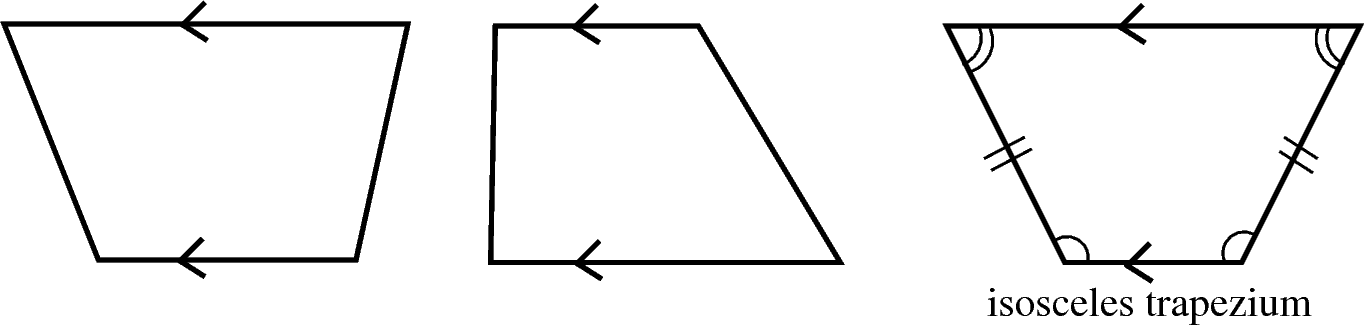
\includegraphics{col11306.imgs/m39354_MG10C13_040.png} % m39354;MG10C13\_040.png;;;6.0;8.5;
        
      \vspace{2pt}
    \vspace{\rubberspace}\par \begin{cnxcaption}
	  \small \textbf{Figure 13.1: }Examples of trapeziums.
	\end{cnxcaption}
      
    \vspace{.1in}
    \rule[.1in]{\figurerulewidth}{.005in} \\
        
    \end{center}

 \end{figure}   

    \addtocounter{footnote}{-0}
    
        
        \label{m39354*uid56}
            \subsubsection{ Parallelogram}
            \nopagebreak
            
          
          \label{m39354*id318843}A trapezium with both sets of opposite sides parallel is called a \textsl{parallelogram}. A summary of the properties of a parallelogram is:\par 
          \label{m39354*id318853}\begin{itemize}[noitemsep]
            \label{m39354*uid57}\item Both pairs of opposite sides are parallel.
\label{m39354*uid58}\item Both pairs of opposite sides are equal in length.
\label{m39354*uid59}\item Both pairs of opposite angles are equal.
\label{m39354*uid60}\item Both diagonals bisect each other (i.e. they cut each other in half).
\end{itemize}
        
          
    \setcounter{subfigure}{0}


	\begin{figure}[H] % horizontal\label{m39354*uid61}
    \begin{center}
    \rule[.1in]{\figurerulewidth}{.005in} \\
        \label{m39354*uid61!!!underscore!!!media}\label{m39354*uid61!!!underscore!!!printimage}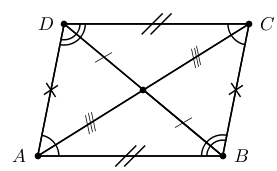
\includegraphics{col11306.imgs/m39354_MG10C13_041.png} % m39354;MG10C13\_041.png;;;6.0;8.5;
        
      \vspace{2pt}
    \vspace{\rubberspace}\par \begin{cnxcaption}
	  \small \textbf{Figure 13.2: }An example of a parallelogram.
	\end{cnxcaption}
      
    \vspace{.1in}
    \rule[.1in]{\figurerulewidth}{.005in} \\
        
    \end{center}

 \end{figure}   

    \addtocounter{footnote}{-0}
    
        
        \label{m39354*uid62}
            \subsubsection{ Rectangle}
            \nopagebreak
            
          
          \label{m39354*id318929}A \textsl{rectangle} is a parallelogram that has all four angles equal to \begin{math}{90}^{\circ }\end{math}. A summary of the properties of a rectangle is:\par 
          \label{m39354*id318954}\begin{itemize}[noitemsep]
            \label{m39354*uid63}\item Both pairs of opposite sides are parallel.
\label{m39354*uid64}\item Both pairs of opposite sides are of equal length.
\label{m39354*uid65}\item Both diagonals bisect each other.
\label{m39354*uid66}\item Diagonals are equal in length.
\label{m39354*uid67}\item All angles at the corners are right angles.
\end{itemize}
        
          
    \setcounter{subfigure}{0}


	\begin{figure}[H] % horizontal\label{m39354*uid68}
    \begin{center}
    \rule[.1in]{\figurerulewidth}{.005in} \\
        \label{m39354*uid68!!!underscore!!!media}\label{m39354*uid68!!!underscore!!!printimage}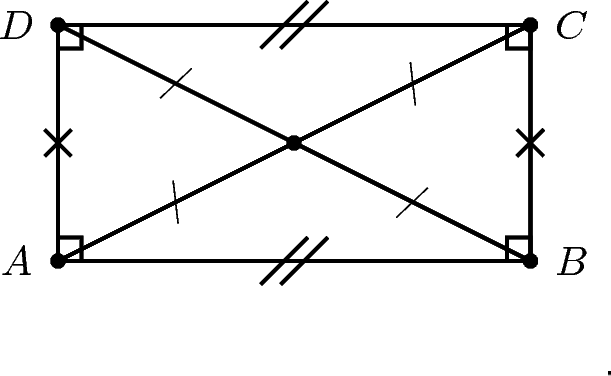
\includegraphics{col11306.imgs/m39354_MG10C13_042.png} % m39354;MG10C13\_042.png;;;6.0;8.5;
        
      \vspace{2pt}
    \vspace{\rubberspace}\par \begin{cnxcaption}
	  \small \textbf{Figure 13.3: }Example of a rectangle.
	\end{cnxcaption}
      
    \vspace{.1in}
    \rule[.1in]{\figurerulewidth}{.005in} \\
        
    \end{center}

 \end{figure}   

    \addtocounter{footnote}{-0}
    
        
        \label{m39354*uid69}
            \subsubsection{ Rhombus}
            \nopagebreak
            
          
          \label{m39354*id319041}A \textsl{rhombus} is a parallelogram that has all four sides of equal length. A summary of the properties of a rhombus is:\par 
          \label{m39354*id319051}\begin{itemize}[noitemsep]
            \label{m39354*uid70}\item Both pairs of opposite sides are parallel.
\label{m39354*uid71}\item All sides are equal in length.
\label{m39354*uid72}\item Both pairs of opposite angles are equal.
\label{m39354*uid73}\item Both diagonals bisect each other at \begin{math}{90}^{\circ }\end{math}.
\label{m39354*uid74}\item Diagonals of a rhombus bisect both pairs of opposite angles.
\end{itemize}
        
          
    \setcounter{subfigure}{0}


	\begin{figure}[H] % horizontal\label{m39354*uid75}
    \begin{center}
    \rule[.1in]{\figurerulewidth}{.005in} \\
        \label{m39354*uid75!!!underscore!!!media}\label{m39354*uid75!!!underscore!!!printimage}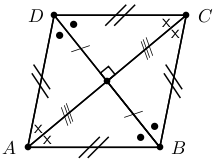
\includegraphics{col11306.imgs/m39354_MG10C13_043.png} % m39354;MG10C13\_043.png;;;6.0;8.5;
        
      \vspace{2pt}
    \vspace{\rubberspace}\par \begin{cnxcaption}
	  \small \textbf{Figure 13.4: }An example of a rhombus. A rhombus is a parallelogram with all sides equal.
	\end{cnxcaption}
      
    \vspace{.1in}
    \rule[.1in]{\figurerulewidth}{.005in} \\
        
    \end{center}

 \end{figure}   

    \addtocounter{footnote}{-0}
    
        
        \label{m39354*uid76}
            \subsubsection{ Square}
            \nopagebreak
            
          
          \label{m39354*id319154}A \textsl{square} is a rhombus that has all four angles equal to 90\begin{math}{}^{\circ }\end{math}.\par 
          \label{m39354*id319177}A summary of the properties of a square is:\par 
          \label{m39354*id319181}\begin{itemize}[noitemsep]
            \label{m39354*uid77}\item Both pairs of opposite sides are parallel.
\label{m39354*uid78}\item All sides are equal in length.
\label{m39354*uid79}\item All angles are equal to \begin{math}{90}^{\circ }\end{math}.
\label{m39354*uid80}\item Both pairs of opposite angles are equal.
\label{m39354*uid81}\item Both diagonals bisect each other at \begin{math}{90}^{\circ }\end{math}.
\label{m39354*uid82}\item Diagonals are equal in length.
\label{m39354*uid83}\item Diagonals bisect both pairs of opposite angles (ie. all \begin{math}{45}^{\circ }\end{math}).
\end{itemize}
        
          
    \setcounter{subfigure}{0}


	\begin{figure}[H] % horizontal\label{m39354*uid84}
    \begin{center}
    \rule[.1in]{\figurerulewidth}{.005in} \\
        \label{m39354*uid84!!!underscore!!!media}\label{m39354*uid84!!!underscore!!!printimage}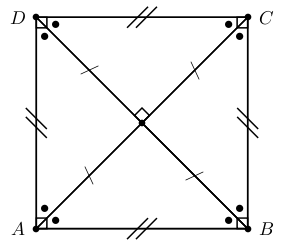
\includegraphics{col11306.imgs/m39354_MG10C13_044.png} % m39354;MG10C13\_044.png;;;6.0;8.5;
        
      \vspace{2pt}
    \vspace{\rubberspace}\par \begin{cnxcaption}
	  \small \textbf{Figure 13.5: }An example of a square. A square is a rhombus with all angles equal to 90\begin{math}{}^{\circ }\end{math}.
	\end{cnxcaption}
      
    \vspace{.1in}
    \rule[.1in]{\figurerulewidth}{.005in} \\
        
    \end{center}

 \end{figure}   

    \addtocounter{footnote}{-0}
    
        
        \label{m39354*uid85}
            \subsubsection{ Kite}
            \nopagebreak
            
          
          \label{m39354*id319349}A \textsl{kite} is a quadrilateral with two pairs of adjacent sides equal.\par 
          \label{m39354*id319359}A summary of the properties of a kite is:\par 
          \label{m39354*id319362}\begin{itemize}[noitemsep]
            \label{m39354*uid86}\item Two pairs of adjacent sides are equal in length.
\label{m39354*uid87}\item One pair of opposite angles are equal where the angles are between unequal sides.
\label{m39354*uid88}\item One diagonal bisects the other diagonal and one diagonal bisects one pair of opposite angles.
\label{m39354*uid89}\item Diagonals intersect at right-angles.
\end{itemize}
        
          
    \setcounter{subfigure}{0}


	\begin{figure}[H] % horizontal\label{m39354*uid90}
    \begin{center}
    \rule[.1in]{\figurerulewidth}{.005in} \\
        \label{m39354*uid90!!!underscore!!!media}\label{m39354*uid90!!!underscore!!!printimage}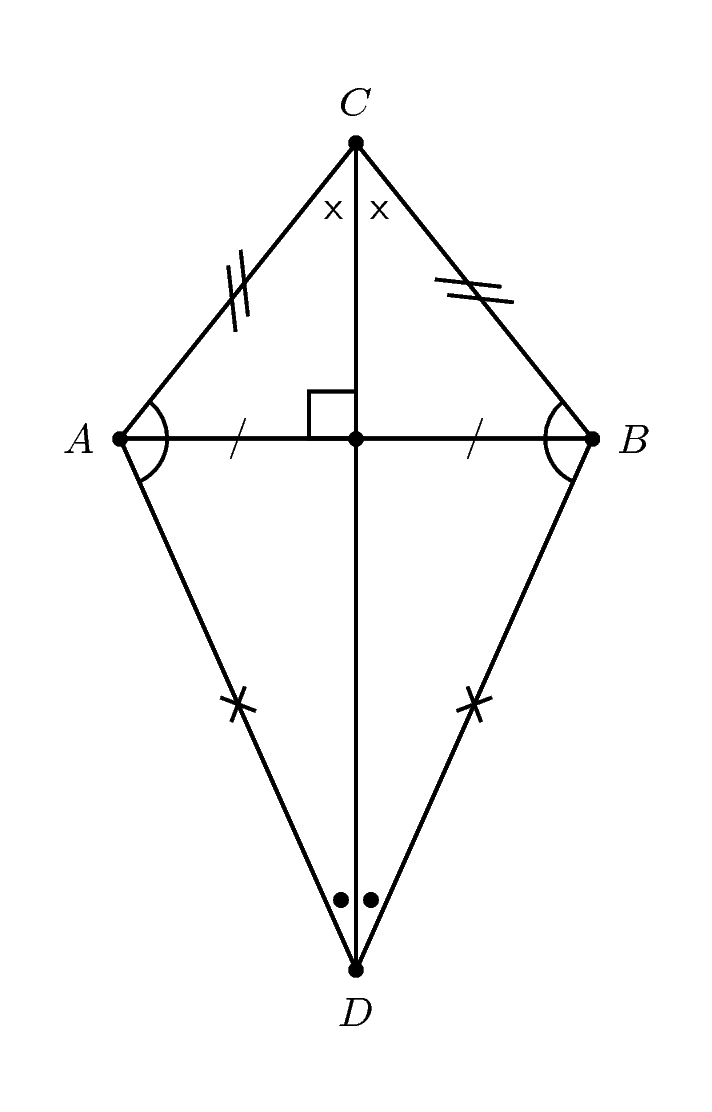
\includegraphics{col11306.imgs/m39354_MG10C13_045.png} % m39354;MG10C13\_045.png;;;6.0;8.5;
        
      \vspace{2pt}
    \vspace{\rubberspace}\par \begin{cnxcaption}
	  \small \textbf{Figure 13.6: }An example of a kite.
	\end{cnxcaption}
      
    \vspace{.1in}
    \rule[.1in]{\figurerulewidth}{.005in} \\
        
    \end{center}

 \end{figure}   

    \addtocounter{footnote}{-0}
    
        
\label{m39354*id9732}Rectangles are a special case (or a subset) of parallelograms. Rectangles are parallelograms that have all angles equal to 90. Squares are a special case (or subset) of rectangles. Squares are rectangles that have all sides equal in length. So all squares are parallelograms and rectangles. So if you are asked to prove that a quadrilateral is a parallelogram, it is enough to show that both pairs of opposite sides are parallel. But if you are asked to prove that a quadrilateral is a square, then you must also show that the angles are all right angles and the sides are equal in length.
\par 
      
      
      \label{m39354*cid4}
            \subsection{ Polygons}
            \nopagebreak
            
      
      \label{m39354*id64553}Polygons are all around us. A stop sign is in the shape of an octagon, an eight-sided polygon. The honeycomb of a beehive consists of hexagonal cells. The top of a desk is a rectangle. Note that although in the first two of these cases the sides of the polygon are all the same, but this need not be the case. Polygons with all sides and angles the same are called 'regular', while those with some sides or angles that are different are called 'irregular'. Although we often work with irregular triangles and quadrilaterals, once one gets up to polygons with greater than four sides, the more interesting ones are often the regular ones.\par 
      \label{m39354*id64557}In this section, you will learn about similar polygons.\par 
      \label{m39354*uid25}
            \subsubsection{ Similarity of Polygons}
            \nopagebreak
            
        
\label{m39354*secfhsst!!!underscore!!!id491}
            \subsubsection{  Discussion : Similar Triangles }
            \nopagebreak
            
        \label{m39354*id64577}Fill in the table using the diagram and then answer the questions that follow.\par 
        
    % \textbf{m39354*id64584}\par
    
    % how many colspecs?  3
          % name: cnx:colspec
            % colnum: 1
            % colwidth: 10*
            % latex-name: columna
            % colname: 
            % align/tgroup-align/default: //left
            % -------------------------
            % name: cnx:colspec
            % colnum: 2
            % colwidth: 10*
            % latex-name: columnb
            % colname: 
            % align/tgroup-align/default: //left
            % -------------------------
            % name: cnx:colspec
            % colnum: 3
            % colwidth: 10*
            % latex-name: columnc
            % colname: 
            % align/tgroup-align/default: //left
            % -------------------------
      
    
    \setlength\mytablespace{6\tabcolsep}
    \addtolength\mytablespace{4\arrayrulewidth}
    \setlength\mytablewidth{\linewidth}
        
    
    \setlength\mytableroom{\mytablewidth}
    \addtolength\mytableroom{-\mytablespace}
    
    \setlength\myfixedwidth{0pt}
    \setlength\mystarwidth{\mytableroom}
        \addtolength\mystarwidth{-\myfixedwidth}
        \divide\mystarwidth 30
        
    
      % ----- Begin capturing width of table in LR mode woof
      \settowidth{\mytableboxwidth}{\begin{tabular}[t]{|l|l|l|}\hline
    % count in rowspan-info-nodeset: 3
    % align/colidx: left,1
    
    % rowcount: '0' | start: 'false' | colidx: '1'
    
        % Formatting a regular cell and recurring on the next sibling
        \begin{math}\frac{\mathrm{AB}}{\mathrm{DE}}\end{math}=\begin{math}\frac{...cm}{...cm}=...\end{math} &
      % align/colidx: left,2
    
    % rowcount: '0' | start: 'false' | colidx: '2'
    
        % Formatting a regular cell and recurring on the next sibling
        \begin{math}\hat{A}\end{math}=...\begin{math}{}^{\circ }\end{math} &
      % align/colidx: left,3
    
    % rowcount: '0' | start: 'false' | colidx: '3'
    
        % Formatting a regular cell and recurring on the next sibling
        \begin{math}\hat{D}\end{math}...\begin{math}{}^{\circ }\end{math}% make-rowspan-placeholders
    % rowspan info: col1 '0' | 'false' | '' || col2 '0' | 'false' | '' || col3 '0' | 'false' | ''
     \tabularnewline\cline{1-1}\cline{2-2}\cline{3-3}
      %--------------------------------------------------------------------
    % align/colidx: left,1
    
    % rowcount: '0' | start: 'false' | colidx: '1'
    
        % Formatting a regular cell and recurring on the next sibling
        \begin{math}\frac{\mathrm{BC}}{\mathrm{EF}}\end{math}=\begin{math}\frac{...cm}{...cm}=...\end{math} &
      % align/colidx: left,2
    
    % rowcount: '0' | start: 'false' | colidx: '2'
    
        % Formatting a regular cell and recurring on the next sibling
        \begin{math}\hat{B}\end{math}=...\begin{math}{}^{\circ }\end{math} &
      % align/colidx: left,3
    
    % rowcount: '0' | start: 'false' | colidx: '3'
    
        % Formatting a regular cell and recurring on the next sibling
        \begin{math}\hat{E}\end{math}=...\begin{math}{}^{\circ }\end{math}% make-rowspan-placeholders
    % rowspan info: col1 '0' | 'false' | '' || col2 '0' | 'false' | '' || col3 '0' | 'false' | ''
     \tabularnewline\cline{1-1}\cline{2-2}\cline{3-3}
      %--------------------------------------------------------------------
    % align/colidx: left,1
    
    % rowcount: '0' | start: 'false' | colidx: '1'
    
        % Formatting a regular cell and recurring on the next sibling
        \begin{math}\frac{\mathrm{AC}}{\mathrm{DF}}\end{math}=\begin{math}\frac{...cm}{...cm}=...\end{math} &
      % align/colidx: left,2
    
    % rowcount: '0' | start: 'false' | colidx: '2'
    
        % Formatting a regular cell and recurring on the next sibling
        \begin{math}\hat{C}\end{math}...\begin{math}{}^{\circ }\end{math} &
      % align/colidx: left,3
    
    % rowcount: '0' | start: 'false' | colidx: '3'
    
        % Formatting a regular cell and recurring on the next sibling
        \begin{math}\hat{F}\end{math}=...\begin{math}{}^{\circ }\end{math}% make-rowspan-placeholders
    % rowspan info: col1 '0' | 'false' | '' || col2 '0' | 'false' | '' || col3 '0' | 'false' | ''
     \tabularnewline\cline{1-1}\cline{2-2}\cline{3-3}
      %--------------------------------------------------------------------
    \end{tabular}} % end mytableboxwidth set
      \addtocounter{footnote}{-0}
      
      % ----- End capturing width of table in LR mode
    
        % ----- LR or paragraph mode: must test
        % ----- Begin capturing height of table
        \settoheight{\mytableboxheight}{\begin{tabular}[t]{|l|l|l|}\hline
    % count in rowspan-info-nodeset: 3
    % align/colidx: left,1
    
    % rowcount: '0' | start: 'false' | colidx: '1'
    
        % Formatting a regular cell and recurring on the next sibling
        \begin{math}\frac{\mathrm{AB}}{\mathrm{DE}}\end{math}=\begin{math}\frac{...cm}{...cm}=...\end{math} &
      % align/colidx: left,2
    
    % rowcount: '0' | start: 'false' | colidx: '2'
    
        % Formatting a regular cell and recurring on the next sibling
        \begin{math}\hat{A}\end{math}=...\begin{math}{}^{\circ }\end{math} &
      % align/colidx: left,3
    
    % rowcount: '0' | start: 'false' | colidx: '3'
    
        % Formatting a regular cell and recurring on the next sibling
        \begin{math}\hat{D}\end{math}...\begin{math}{}^{\circ }\end{math}% make-rowspan-placeholders
    % rowspan info: col1 '0' | 'false' | '' || col2 '0' | 'false' | '' || col3 '0' | 'false' | ''
     \tabularnewline\cline{1-1}\cline{2-2}\cline{3-3}
      %--------------------------------------------------------------------
    % align/colidx: left,1
    
    % rowcount: '0' | start: 'false' | colidx: '1'
    
        % Formatting a regular cell and recurring on the next sibling
        \begin{math}\frac{\mathrm{BC}}{\mathrm{EF}}\end{math}=\begin{math}\frac{...cm}{...cm}=...\end{math} &
      % align/colidx: left,2
    
    % rowcount: '0' | start: 'false' | colidx: '2'
    
        % Formatting a regular cell and recurring on the next sibling
        \begin{math}\hat{B}\end{math}=...\begin{math}{}^{\circ }\end{math} &
      % align/colidx: left,3
    
    % rowcount: '0' | start: 'false' | colidx: '3'
    
        % Formatting a regular cell and recurring on the next sibling
        \begin{math}\hat{E}\end{math}=...\begin{math}{}^{\circ }\end{math}% make-rowspan-placeholders
    % rowspan info: col1 '0' | 'false' | '' || col2 '0' | 'false' | '' || col3 '0' | 'false' | ''
     \tabularnewline\cline{1-1}\cline{2-2}\cline{3-3}
      %--------------------------------------------------------------------
    % align/colidx: left,1
    
    % rowcount: '0' | start: 'false' | colidx: '1'
    
        % Formatting a regular cell and recurring on the next sibling
        \begin{math}\frac{\mathrm{AC}}{\mathrm{DF}}\end{math}=\begin{math}\frac{...cm}{...cm}=...\end{math} &
      % align/colidx: left,2
    
    % rowcount: '0' | start: 'false' | colidx: '2'
    
        % Formatting a regular cell and recurring on the next sibling
        \begin{math}\hat{C}\end{math}...\begin{math}{}^{\circ }\end{math} &
      % align/colidx: left,3
    
    % rowcount: '0' | start: 'false' | colidx: '3'
    
        % Formatting a regular cell and recurring on the next sibling
        \begin{math}\hat{F}\end{math}=...\begin{math}{}^{\circ }\end{math}% make-rowspan-placeholders
    % rowspan info: col1 '0' | 'false' | '' || col2 '0' | 'false' | '' || col3 '0' | 'false' | ''
     \tabularnewline\cline{1-1}\cline{2-2}\cline{3-3}
      %--------------------------------------------------------------------
    \end{tabular}} % end mytableboxheight set
        \settodepth{\mytableboxdepth}{\begin{tabular}[t]{|l|l|l|}\hline
    % count in rowspan-info-nodeset: 3
    % align/colidx: left,1
    
    % rowcount: '0' | start: 'false' | colidx: '1'
    
        % Formatting a regular cell and recurring on the next sibling
        \begin{math}\frac{\mathrm{AB}}{\mathrm{DE}}\end{math}=\begin{math}\frac{...cm}{...cm}=...\end{math} &
      % align/colidx: left,2
    
    % rowcount: '0' | start: 'false' | colidx: '2'
    
        % Formatting a regular cell and recurring on the next sibling
        \begin{math}\hat{A}\end{math}=...\begin{math}{}^{\circ }\end{math} &
      % align/colidx: left,3
    
    % rowcount: '0' | start: 'false' | colidx: '3'
    
        % Formatting a regular cell and recurring on the next sibling
        \begin{math}\hat{D}\end{math}...\begin{math}{}^{\circ }\end{math}% make-rowspan-placeholders
    % rowspan info: col1 '0' | 'false' | '' || col2 '0' | 'false' | '' || col3 '0' | 'false' | ''
     \tabularnewline\cline{1-1}\cline{2-2}\cline{3-3}
      %--------------------------------------------------------------------
    % align/colidx: left,1
    
    % rowcount: '0' | start: 'false' | colidx: '1'
    
        % Formatting a regular cell and recurring on the next sibling
        \begin{math}\frac{\mathrm{BC}}{\mathrm{EF}}\end{math}=\begin{math}\frac{...cm}{...cm}=...\end{math} &
      % align/colidx: left,2
    
    % rowcount: '0' | start: 'false' | colidx: '2'
    
        % Formatting a regular cell and recurring on the next sibling
        \begin{math}\hat{B}\end{math}=...\begin{math}{}^{\circ }\end{math} &
      % align/colidx: left,3
    
    % rowcount: '0' | start: 'false' | colidx: '3'
    
        % Formatting a regular cell and recurring on the next sibling
        \begin{math}\hat{E}\end{math}=...\begin{math}{}^{\circ }\end{math}% make-rowspan-placeholders
    % rowspan info: col1 '0' | 'false' | '' || col2 '0' | 'false' | '' || col3 '0' | 'false' | ''
     \tabularnewline\cline{1-1}\cline{2-2}\cline{3-3}
      %--------------------------------------------------------------------
    % align/colidx: left,1
    
    % rowcount: '0' | start: 'false' | colidx: '1'
    
        % Formatting a regular cell and recurring on the next sibling
        \begin{math}\frac{\mathrm{AC}}{\mathrm{DF}}\end{math}=\begin{math}\frac{...cm}{...cm}=...\end{math} &
      % align/colidx: left,2
    
    % rowcount: '0' | start: 'false' | colidx: '2'
    
        % Formatting a regular cell and recurring on the next sibling
        \begin{math}\hat{C}\end{math}...\begin{math}{}^{\circ }\end{math} &
      % align/colidx: left,3
    
    % rowcount: '0' | start: 'false' | colidx: '3'
    
        % Formatting a regular cell and recurring on the next sibling
        \begin{math}\hat{F}\end{math}=...\begin{math}{}^{\circ }\end{math}% make-rowspan-placeholders
    % rowspan info: col1 '0' | 'false' | '' || col2 '0' | 'false' | '' || col3 '0' | 'false' | ''
     \tabularnewline\cline{1-1}\cline{2-2}\cline{3-3}
      %--------------------------------------------------------------------
    \end{tabular}} % end mytableboxdepth set
        \addtolength{\mytableboxheight}{\mytableboxdepth}
        % ----- End capturing height of table
        \addtocounter{footnote}{-0}
        
        \ifthenelse{\mytableboxwidth<\textwidth}{% the table fits in LR mode
          \addtolength{\mytableboxwidth}{-\mytablespace}
          \typeout{textheight: \the\textheight}
          \typeout{mytableboxheight: \the\mytableboxheight}
          \typeout{textwidth: \the\textwidth}
          \typeout{mytableboxwidth: \the\mytableboxwidth}
          \ifthenelse{\mytableboxheight<\textheight}{%
        
    % \begin{table}[H]
    % \\ '' '0'
    
        \begin{center}
      
      \label{m39354*id64584}
      
    \noindent
    \begin{tabular}[t]{|l|l|l|}\hline
    % count in rowspan-info-nodeset: 3
    % align/colidx: left,1
    
    % rowcount: '0' | start: 'false' | colidx: '1'
    
        % Formatting a regular cell and recurring on the next sibling
        \begin{math}\frac{\mathrm{AB}}{\mathrm{DE}}\end{math}=\begin{math}\frac{...cm}{...cm}=...\end{math} &
      % align/colidx: left,2
    
    % rowcount: '0' | start: 'false' | colidx: '2'
    
        % Formatting a regular cell and recurring on the next sibling
        \begin{math}\hat{A}\end{math}=...\begin{math}{}^{\circ }\end{math} &
      % align/colidx: left,3
    
    % rowcount: '0' | start: 'false' | colidx: '3'
    
        % Formatting a regular cell and recurring on the next sibling
        \begin{math}\hat{D}\end{math}...\begin{math}{}^{\circ }\end{math}% make-rowspan-placeholders
    % rowspan info: col1 '0' | 'false' | '' || col2 '0' | 'false' | '' || col3 '0' | 'false' | ''
     \tabularnewline\cline{1-1}\cline{2-2}\cline{3-3}
      %--------------------------------------------------------------------
    % align/colidx: left,1
    
    % rowcount: '0' | start: 'false' | colidx: '1'
    
        % Formatting a regular cell and recurring on the next sibling
        \begin{math}\frac{\mathrm{BC}}{\mathrm{EF}}\end{math}=\begin{math}\frac{...cm}{...cm}=...\end{math} &
      % align/colidx: left,2
    
    % rowcount: '0' | start: 'false' | colidx: '2'
    
        % Formatting a regular cell and recurring on the next sibling
        \begin{math}\hat{B}\end{math}=...\begin{math}{}^{\circ }\end{math} &
      % align/colidx: left,3
    
    % rowcount: '0' | start: 'false' | colidx: '3'
    
        % Formatting a regular cell and recurring on the next sibling
        \begin{math}\hat{E}\end{math}=...\begin{math}{}^{\circ }\end{math}% make-rowspan-placeholders
    % rowspan info: col1 '0' | 'false' | '' || col2 '0' | 'false' | '' || col3 '0' | 'false' | ''
     \tabularnewline\cline{1-1}\cline{2-2}\cline{3-3}
      %--------------------------------------------------------------------
    % align/colidx: left,1
    
    % rowcount: '0' | start: 'false' | colidx: '1'
    
        % Formatting a regular cell and recurring on the next sibling
        \begin{math}\frac{\mathrm{AC}}{\mathrm{DF}}\end{math}=\begin{math}\frac{...cm}{...cm}=...\end{math} &
      % align/colidx: left,2
    
    % rowcount: '0' | start: 'false' | colidx: '2'
    
        % Formatting a regular cell and recurring on the next sibling
        \begin{math}\hat{C}\end{math}...\begin{math}{}^{\circ }\end{math} &
      % align/colidx: left,3
    
    % rowcount: '0' | start: 'false' | colidx: '3'
    
        % Formatting a regular cell and recurring on the next sibling
        \begin{math}\hat{F}\end{math}=...\begin{math}{}^{\circ }\end{math}% make-rowspan-placeholders
    % rowspan info: col1 '0' | 'false' | '' || col2 '0' | 'false' | '' || col3 '0' | 'false' | ''
     \tabularnewline\cline{1-1}\cline{2-2}\cline{3-3}
      %--------------------------------------------------------------------
    \end{tabular}
      \end{center}
    \begin{center}{\small\bfseries Table 13.1}\end{center}
    %\end{table}
    
    \addtocounter{footnote}{-0}
    
          }{ % else
        
    % \begin{table}[H]
    % \\ '' '0'
    
        \begin{center}
      
      \label{m39354*id64584}
      
    \noindent
    \tabletail{%
        \hline
        \multicolumn{3}{|p{\mytableboxwidth}|}{\raggedleft \small \sl continued on next page}\\
        \hline
      }
      \tablelasttail{}
      \begin{xtabular}[t]{|l|l|l|}\hline
    % count in rowspan-info-nodeset: 3
    % align/colidx: left,1
    
    % rowcount: '0' | start: 'false' | colidx: '1'
    
        % Formatting a regular cell and recurring on the next sibling
        \begin{math}\frac{\mathrm{AB}}{\mathrm{DE}}\end{math}=\begin{math}\frac{...cm}{...cm}=...\end{math} &
      % align/colidx: left,2
    
    % rowcount: '0' | start: 'false' | colidx: '2'
    
        % Formatting a regular cell and recurring on the next sibling
        \begin{math}\hat{A}\end{math}=...\begin{math}{}^{\circ }\end{math} &
      % align/colidx: left,3
    
    % rowcount: '0' | start: 'false' | colidx: '3'
    
        % Formatting a regular cell and recurring on the next sibling
        \begin{math}\hat{D}\end{math}...\begin{math}{}^{\circ }\end{math}% make-rowspan-placeholders
    % rowspan info: col1 '0' | 'false' | '' || col2 '0' | 'false' | '' || col3 '0' | 'false' | ''
     \tabularnewline\cline{1-1}\cline{2-2}\cline{3-3}
      %--------------------------------------------------------------------
    % align/colidx: left,1
    
    % rowcount: '0' | start: 'false' | colidx: '1'
    
        % Formatting a regular cell and recurring on the next sibling
        \begin{math}\frac{\mathrm{BC}}{\mathrm{EF}}\end{math}=\begin{math}\frac{...cm}{...cm}=...\end{math} &
      % align/colidx: left,2
    
    % rowcount: '0' | start: 'false' | colidx: '2'
    
        % Formatting a regular cell and recurring on the next sibling
        \begin{math}\hat{B}\end{math}=...\begin{math}{}^{\circ }\end{math} &
      % align/colidx: left,3
    
    % rowcount: '0' | start: 'false' | colidx: '3'
    
        % Formatting a regular cell and recurring on the next sibling
        \begin{math}\hat{E}\end{math}=...\begin{math}{}^{\circ }\end{math}% make-rowspan-placeholders
    % rowspan info: col1 '0' | 'false' | '' || col2 '0' | 'false' | '' || col3 '0' | 'false' | ''
     \tabularnewline\cline{1-1}\cline{2-2}\cline{3-3}
      %--------------------------------------------------------------------
    % align/colidx: left,1
    
    % rowcount: '0' | start: 'false' | colidx: '1'
    
        % Formatting a regular cell and recurring on the next sibling
        \begin{math}\frac{\mathrm{AC}}{\mathrm{DF}}\end{math}=\begin{math}\frac{...cm}{...cm}=...\end{math} &
      % align/colidx: left,2
    
    % rowcount: '0' | start: 'false' | colidx: '2'
    
        % Formatting a regular cell and recurring on the next sibling
        \begin{math}\hat{C}\end{math}...\begin{math}{}^{\circ }\end{math} &
      % align/colidx: left,3
    
    % rowcount: '0' | start: 'false' | colidx: '3'
    
        % Formatting a regular cell and recurring on the next sibling
        \begin{math}\hat{F}\end{math}=...\begin{math}{}^{\circ }\end{math}% make-rowspan-placeholders
    % rowspan info: col1 '0' | 'false' | '' || col2 '0' | 'false' | '' || col3 '0' | 'false' | ''
     \tabularnewline\cline{1-1}\cline{2-2}\cline{3-3}
      %--------------------------------------------------------------------
    \end{xtabular}
      \end{center}
    \begin{center}{\small\bfseries Table 13.1}\end{center}
    %\end{table}
    
    \addtocounter{footnote}{-0}
    
          } % 
        }{% else
        % typeset the table in paragraph mode
        % ----- Begin capturing height of table
        \settoheight{\mytableboxheight}{\begin{tabular*}{\mytablewidth}[t]{|p{10\mystarwidth}|p{10\mystarwidth}|p{10\mystarwidth}|}\hline
    % count in rowspan-info-nodeset: 3
    % align/colidx: left,1
    
    % rowcount: '0' | start: 'false' | colidx: '1'
    
        % Formatting a regular cell and recurring on the next sibling
        \begin{math}\frac{\mathrm{AB}}{\mathrm{DE}}\end{math}=\begin{math}\frac{...cm}{...cm}=...\end{math} &
      % align/colidx: left,2
    
    % rowcount: '0' | start: 'false' | colidx: '2'
    
        % Formatting a regular cell and recurring on the next sibling
        \begin{math}\hat{A}\end{math}=...\begin{math}{}^{\circ }\end{math} &
      % align/colidx: left,3
    
    % rowcount: '0' | start: 'false' | colidx: '3'
    
        % Formatting a regular cell and recurring on the next sibling
        \begin{math}\hat{D}\end{math}...\begin{math}{}^{\circ }\end{math}% make-rowspan-placeholders
    % rowspan info: col1 '0' | 'false' | '' || col2 '0' | 'false' | '' || col3 '0' | 'false' | ''
     \tabularnewline\cline{1-1}\cline{2-2}\cline{3-3}
      %--------------------------------------------------------------------
    % align/colidx: left,1
    
    % rowcount: '0' | start: 'false' | colidx: '1'
    
        % Formatting a regular cell and recurring on the next sibling
        \begin{math}\frac{\mathrm{BC}}{\mathrm{EF}}\end{math}=\begin{math}\frac{...cm}{...cm}=...\end{math} &
      % align/colidx: left,2
    
    % rowcount: '0' | start: 'false' | colidx: '2'
    
        % Formatting a regular cell and recurring on the next sibling
        \begin{math}\hat{B}\end{math}=...\begin{math}{}^{\circ }\end{math} &
      % align/colidx: left,3
    
    % rowcount: '0' | start: 'false' | colidx: '3'
    
        % Formatting a regular cell and recurring on the next sibling
        \begin{math}\hat{E}\end{math}=...\begin{math}{}^{\circ }\end{math}% make-rowspan-placeholders
    % rowspan info: col1 '0' | 'false' | '' || col2 '0' | 'false' | '' || col3 '0' | 'false' | ''
     \tabularnewline\cline{1-1}\cline{2-2}\cline{3-3}
      %--------------------------------------------------------------------
    % align/colidx: left,1
    
    % rowcount: '0' | start: 'false' | colidx: '1'
    
        % Formatting a regular cell and recurring on the next sibling
        \begin{math}\frac{\mathrm{AC}}{\mathrm{DF}}\end{math}=\begin{math}\frac{...cm}{...cm}=...\end{math} &
      % align/colidx: left,2
    
    % rowcount: '0' | start: 'false' | colidx: '2'
    
        % Formatting a regular cell and recurring on the next sibling
        \begin{math}\hat{C}\end{math}...\begin{math}{}^{\circ }\end{math} &
      % align/colidx: left,3
    
    % rowcount: '0' | start: 'false' | colidx: '3'
    
        % Formatting a regular cell and recurring on the next sibling
        \begin{math}\hat{F}\end{math}=...\begin{math}{}^{\circ }\end{math}% make-rowspan-placeholders
    % rowspan info: col1 '0' | 'false' | '' || col2 '0' | 'false' | '' || col3 '0' | 'false' | ''
     \tabularnewline\cline{1-1}\cline{2-2}\cline{3-3}
      %--------------------------------------------------------------------
    \end{tabular*}} % end mytableboxheight set
        \settodepth{\mytableboxdepth}{\begin{tabular*}{\mytablewidth}[t]{|p{10\mystarwidth}|p{10\mystarwidth}|p{10\mystarwidth}|}\hline
    % count in rowspan-info-nodeset: 3
    % align/colidx: left,1
    
    % rowcount: '0' | start: 'false' | colidx: '1'
    
        % Formatting a regular cell and recurring on the next sibling
        \begin{math}\frac{\mathrm{AB}}{\mathrm{DE}}\end{math}=\begin{math}\frac{...cm}{...cm}=...\end{math} &
      % align/colidx: left,2
    
    % rowcount: '0' | start: 'false' | colidx: '2'
    
        % Formatting a regular cell and recurring on the next sibling
        \begin{math}\hat{A}\end{math}=...\begin{math}{}^{\circ }\end{math} &
      % align/colidx: left,3
    
    % rowcount: '0' | start: 'false' | colidx: '3'
    
        % Formatting a regular cell and recurring on the next sibling
        \begin{math}\hat{D}\end{math}...\begin{math}{}^{\circ }\end{math}% make-rowspan-placeholders
    % rowspan info: col1 '0' | 'false' | '' || col2 '0' | 'false' | '' || col3 '0' | 'false' | ''
     \tabularnewline\cline{1-1}\cline{2-2}\cline{3-3}
      %--------------------------------------------------------------------
    % align/colidx: left,1
    
    % rowcount: '0' | start: 'false' | colidx: '1'
    
        % Formatting a regular cell and recurring on the next sibling
        \begin{math}\frac{\mathrm{BC}}{\mathrm{EF}}\end{math}=\begin{math}\frac{...cm}{...cm}=...\end{math} &
      % align/colidx: left,2
    
    % rowcount: '0' | start: 'false' | colidx: '2'
    
        % Formatting a regular cell and recurring on the next sibling
        \begin{math}\hat{B}\end{math}=...\begin{math}{}^{\circ }\end{math} &
      % align/colidx: left,3
    
    % rowcount: '0' | start: 'false' | colidx: '3'
    
        % Formatting a regular cell and recurring on the next sibling
        \begin{math}\hat{E}\end{math}=...\begin{math}{}^{\circ }\end{math}% make-rowspan-placeholders
    % rowspan info: col1 '0' | 'false' | '' || col2 '0' | 'false' | '' || col3 '0' | 'false' | ''
     \tabularnewline\cline{1-1}\cline{2-2}\cline{3-3}
      %--------------------------------------------------------------------
    % align/colidx: left,1
    
    % rowcount: '0' | start: 'false' | colidx: '1'
    
        % Formatting a regular cell and recurring on the next sibling
        \begin{math}\frac{\mathrm{AC}}{\mathrm{DF}}\end{math}=\begin{math}\frac{...cm}{...cm}=...\end{math} &
      % align/colidx: left,2
    
    % rowcount: '0' | start: 'false' | colidx: '2'
    
        % Formatting a regular cell and recurring on the next sibling
        \begin{math}\hat{C}\end{math}...\begin{math}{}^{\circ }\end{math} &
      % align/colidx: left,3
    
    % rowcount: '0' | start: 'false' | colidx: '3'
    
        % Formatting a regular cell and recurring on the next sibling
        \begin{math}\hat{F}\end{math}=...\begin{math}{}^{\circ }\end{math}% make-rowspan-placeholders
    % rowspan info: col1 '0' | 'false' | '' || col2 '0' | 'false' | '' || col3 '0' | 'false' | ''
     \tabularnewline\cline{1-1}\cline{2-2}\cline{3-3}
      %--------------------------------------------------------------------
    \end{tabular*}} % end mytableboxdepth set
        \addtolength{\mytableboxheight}{\mytableboxdepth}
        % ----- End capturing height of table
        \typeout{textheight: \the\textheight}
        \typeout{mytableboxheight: \the\mytableboxheight}
        \typeout{table too wide, outputting in para mode}
        
    % \begin{table}[H]
    % \\ '' '0'
    
        \begin{center}
      
      \label{m39354*id64584}
      
    \noindent
    \tabletail{%
        \hline
        \multicolumn{3}{|p{\mytableroom}|}{\raggedleft \small \sl continued on next page}\\
        \hline
      }
      \tablelasttail{}
      \begin{xtabular*}{\mytablewidth}[t]{|p{10\mystarwidth}|p{10\mystarwidth}|p{10\mystarwidth}|}\hline
    % count in rowspan-info-nodeset: 3
    % align/colidx: left,1
    
    % rowcount: '0' | start: 'false' | colidx: '1'
    
        % Formatting a regular cell and recurring on the next sibling
        \begin{math}\frac{\mathrm{AB}}{\mathrm{DE}}\end{math}=\begin{math}\frac{...cm}{...cm}=...\end{math} &
      % align/colidx: left,2
    
    % rowcount: '0' | start: 'false' | colidx: '2'
    
        % Formatting a regular cell and recurring on the next sibling
        \begin{math}\hat{A}\end{math}=...\begin{math}{}^{\circ }\end{math} &
      % align/colidx: left,3
    
    % rowcount: '0' | start: 'false' | colidx: '3'
    
        % Formatting a regular cell and recurring on the next sibling
        \begin{math}\hat{D}\end{math}...\begin{math}{}^{\circ }\end{math}% make-rowspan-placeholders
    % rowspan info: col1 '0' | 'false' | '' || col2 '0' | 'false' | '' || col3 '0' | 'false' | ''
     \tabularnewline\cline{1-1}\cline{2-2}\cline{3-3}
      %--------------------------------------------------------------------
    % align/colidx: left,1
    
    % rowcount: '0' | start: 'false' | colidx: '1'
    
        % Formatting a regular cell and recurring on the next sibling
        \begin{math}\frac{\mathrm{BC}}{\mathrm{EF}}\end{math}=\begin{math}\frac{...cm}{...cm}=...\end{math} &
      % align/colidx: left,2
    
    % rowcount: '0' | start: 'false' | colidx: '2'
    
        % Formatting a regular cell and recurring on the next sibling
        \begin{math}\hat{B}\end{math}=...\begin{math}{}^{\circ }\end{math} &
      % align/colidx: left,3
    
    % rowcount: '0' | start: 'false' | colidx: '3'
    
        % Formatting a regular cell and recurring on the next sibling
        \begin{math}\hat{E}\end{math}=...\begin{math}{}^{\circ }\end{math}% make-rowspan-placeholders
    % rowspan info: col1 '0' | 'false' | '' || col2 '0' | 'false' | '' || col3 '0' | 'false' | ''
     \tabularnewline\cline{1-1}\cline{2-2}\cline{3-3}
      %--------------------------------------------------------------------
    % align/colidx: left,1
    
    % rowcount: '0' | start: 'false' | colidx: '1'
    
        % Formatting a regular cell and recurring on the next sibling
        \begin{math}\frac{\mathrm{AC}}{\mathrm{DF}}\end{math}=\begin{math}\frac{...cm}{...cm}=...\end{math} &
      % align/colidx: left,2
    
    % rowcount: '0' | start: 'false' | colidx: '2'
    
        % Formatting a regular cell and recurring on the next sibling
        \begin{math}\hat{C}\end{math}...\begin{math}{}^{\circ }\end{math} &
      % align/colidx: left,3
    
    % rowcount: '0' | start: 'false' | colidx: '3'
    
        % Formatting a regular cell and recurring on the next sibling
        \begin{math}\hat{F}\end{math}=...\begin{math}{}^{\circ }\end{math}% make-rowspan-placeholders
    % rowspan info: col1 '0' | 'false' | '' || col2 '0' | 'false' | '' || col3 '0' | 'false' | ''
     \tabularnewline\cline{1-1}\cline{2-2}\cline{3-3}
      %--------------------------------------------------------------------
    \end{xtabular*}
      \end{center}
    \begin{center}{\small\bfseries Table 13.1}\end{center}
    %\end{table}
    
    \addtocounter{footnote}{-0}
    
        }% ending lr/para test clause
      
    \par
  
        
        \label{m39354*id65008}
          
    \setcounter{subfigure}{0}


	\begin{figure}[H] % horizontal\label{m39354*id65011}
    \begin{center}
    \label{m39354*id65011!!!underscore!!!media}\label{m39354*id65011!!!underscore!!!printimage}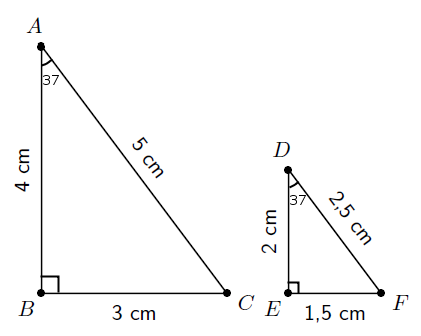
\includegraphics[width=300px]{col11306.imgs/m39354_MG10C14_010.png} % m39354;MG10C14\_010.png;;;6.0;8.5;
        
      \vspace{2pt}
    \vspace{.1in}
    
    \end{center}

 \end{figure}   

    \addtocounter{footnote}{-0}
    
        \par 
        \label{m39354*id65017}\begin{enumerate}[noitemsep, label=\textbf{\arabic*}. ] 
            \label{m39354*uid26}\item What can you say about the numbers you calculated for: \begin{math}\frac{\mathrm{AB}}{\mathrm{DE}}\end{math}, \begin{math}\frac{\mathrm{BC}}{\mathrm{EF}}\end{math}, \begin{math}\frac{\mathrm{AC}}{\mathrm{DF}}\end{math}?
\label{m39354*uid27}\item What can you say about \begin{math}\hat{A}\end{math} and \begin{math}\hat{D}\end{math}?
\label{m39354*uid28}\item What can you say about \begin{math}\hat{B}\end{math} and \begin{math}\hat{E}\end{math}?
\label{m39354*uid29}\item What can you say about \begin{math}\hat{C}\end{math} and \begin{math}\hat{F}\end{math}?
\end{enumerate}
        
        

        \label{m39354*id65212}If two polygons are \textsl{similar}, one is an enlargement of the other. This means that the two polygons will have the same angles and their sides will be in the same proportion.\par 
        \label{m39354*id65223}We use the symbol \begin{math}|||\end{math} to mean \textsl{is similar to}.\par 
\label{m39354*fhsst!!!underscore!!!id537}\begin{definition}
	  \begin{tabular*}{15 cm}{m{15 mm}m{}}
	\hspace*{-50pt}  
\includegraphics[width=0.5in]{col11306.imgs/psflag2.png}   & \Definition{   \label{id2573375}\textbf{ Similar Polygons }} { \label{m39354*meaningfhsst!!!underscore!!!id537}
        \label{m39354*id65247}Two polygons are similar if:\par 
        \label{m39354*id65253}\begin{enumerate}[noitemsep, label=\textbf{\arabic*}. ] 
            \leftskip=20pt\rightskip=\leftskip\label{m39354*uid30}\item their corresponding angles are equal, \textbf{and}\label{m39354*uid31}\item the ratios of corresponding sides are equal.
\end{enumerate}
        
        
         } 
      \end{tabular*}
      \end{definition}

\par
            \label{m39354*secfhsst!!!underscore!!!id546}\vspace{.5cm} 
      
      \noindent
      \hspace*{-30pt}
\includegraphics[width=0.5in]{col11306.imgs/pspencil2.png}   \raisebox{25mm}{   
      \begin{mdframed}[linewidth=4, leftmargin=40, rightmargin=40]  
      \begin{exercise}
    \noindent\textbf{Exercise 13.1:  Similarity of Polygons }
        \label{m39354*probfhsst!!!underscore!!!id547}
        \label{m39354*id65309}Show that the following two polygons are similar.\par 
        \label{m39354*id65315}
          
    \setcounter{subfigure}{0}


	\begin{figure}[H] % horizontal\label{m39354*id65318}
    \begin{center}
    \label{m39354*id65318!!!underscore!!!media}\label{m39354*id65318!!!underscore!!!printimage}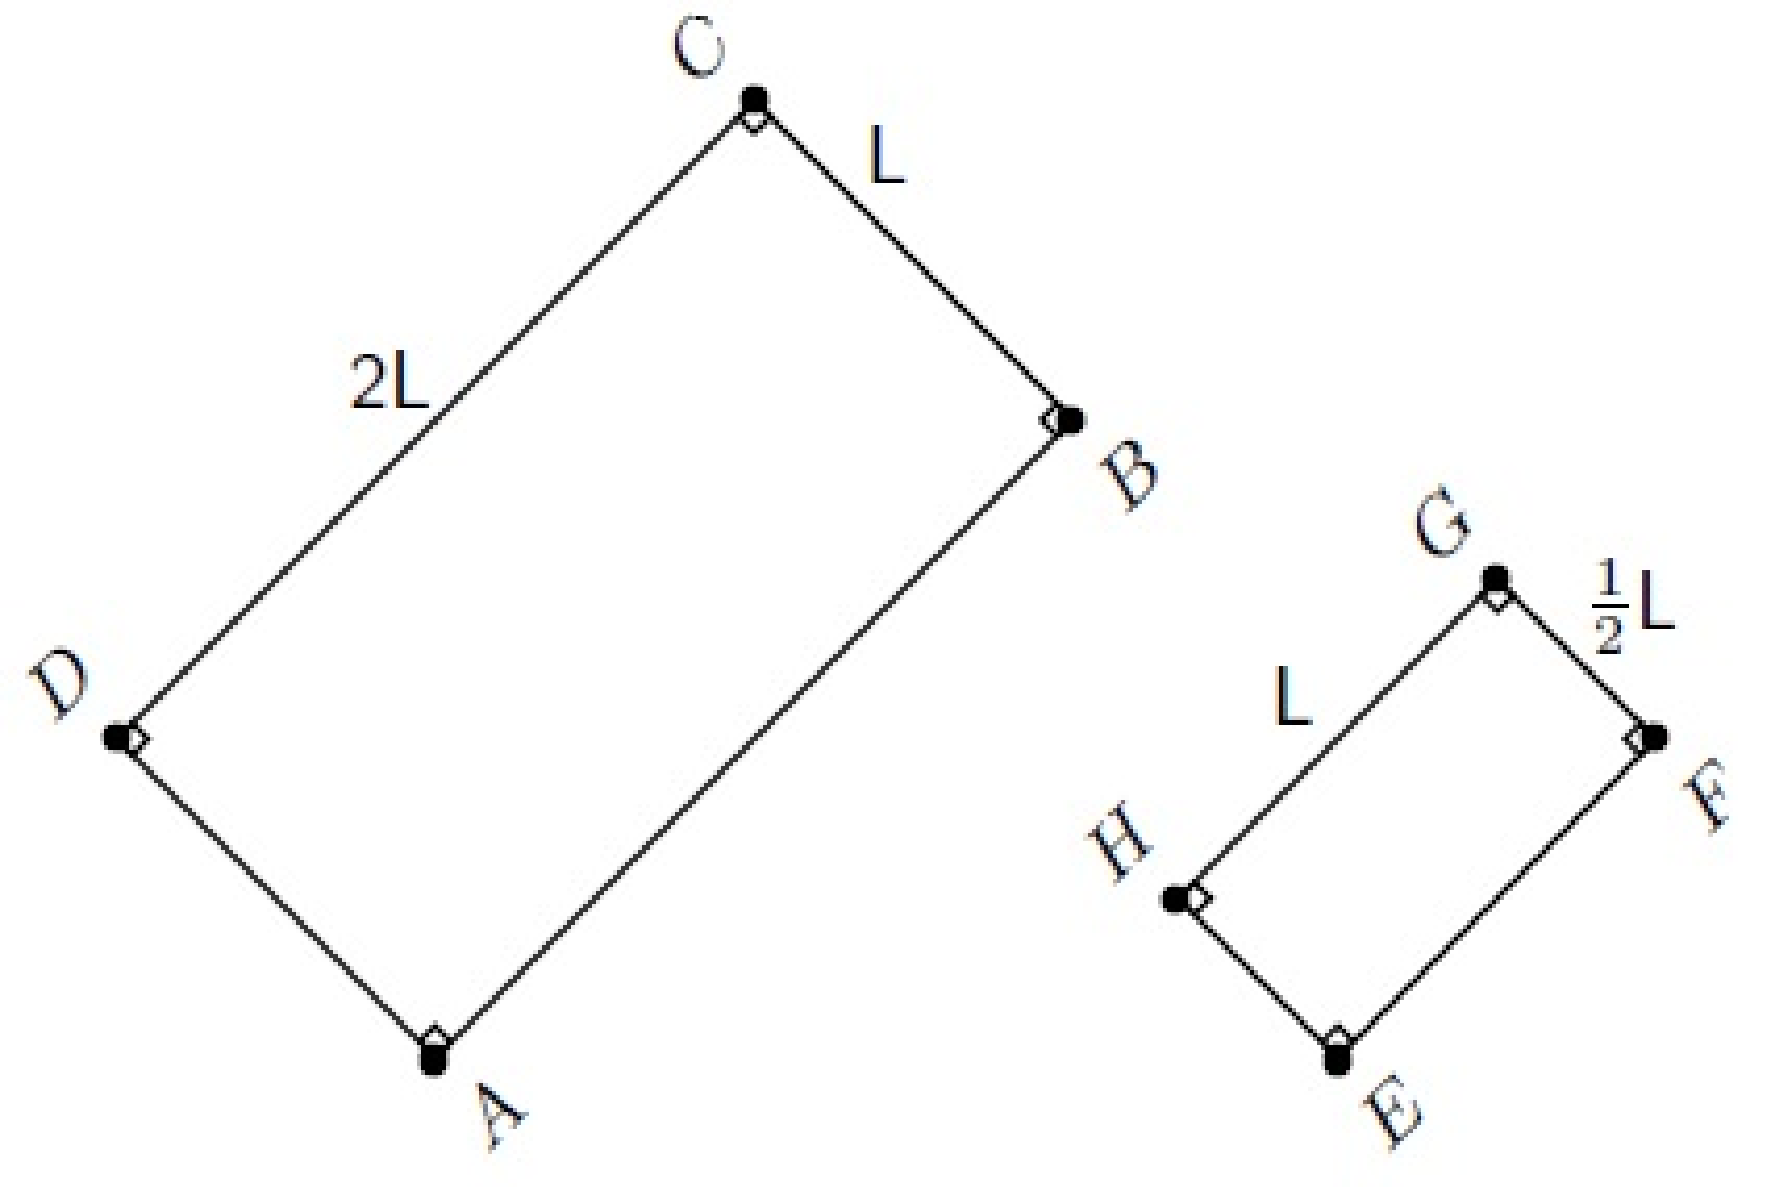
\includegraphics[width=300px]{col11306.imgs/m39354_MG10C14_011.png} % m39354;MG10C14\_011.png;;;6.0;8.5;
        
      \vspace{2pt}
    \vspace{.1in}
    
    \end{center}

 \end{figure}   

    \addtocounter{footnote}{-0}
    
        \par 
        
        \vspace{5pt}
        \label{m39354*solfhsst!!!underscore!!!id559}\noindent\textbf{Solution to Exercise } \label{m39354*listfhsst!!!underscore!!!id559}\begin{enumerate}[noitemsep, label=\textbf{Step} \textbf{\arabic*}. ] 
            \leftskip=20pt\rightskip=\leftskip\item  
        \label{m39354*id65346}We are required to show that the pair of polygons is similar. We can do this by showing that the ratio of corresponding sides is equal and by showing that corresponding angles are equal.\par 
        \item  
        \label{m39354*id65355}We are given the angles. So, we can show that corresponding angles are equal.\par 
        \item  
        \label{m39354*id65363}All angles are given to be 90\begin{math}{}^{\circ }\end{math} and\par 
        \label{m39354*id65380}\nopagebreak\noindent{}
          \settowidth{\mymathboxwidth}{\begin{equation}
    \begin{array}{ccc}\hfill \hat{A}& =& \hat{E}\hfill \\ \hfill \hat{B}& =& \hat{F}\hfill \\ \hfill \hat{C}& =& \hat{G}\hfill \\ \hfill \hat{D}& =& \hat{H}\hfill \end{array}\tag{13.1}
      \end{equation}
    }
    \typeout{Columnwidth = \the\columnwidth}\typeout{math as usual width = \the\mymathboxwidth}
    \ifthenelse{\lengthtest{\mymathboxwidth < \columnwidth}}{% if the math fits, do it again, for real
    \begin{equation}
    \begin{array}{ccc}\hfill \hat{A}& =& \hat{E}\hfill \\ \hfill \hat{B}& =& \hat{F}\hfill \\ \hfill \hat{C}& =& \hat{G}\hfill \\ \hfill \hat{D}& =& \hat{H}\hfill \end{array}\tag{13.1}
      \end{equation}
    }{% else, if it doesn't fit
    \setlength{\mymathboxwidth}{\columnwidth}
      \addtolength{\mymathboxwidth}{-48pt}
    \par\vspace{12pt}\noindent\begin{minipage}{\columnwidth}
    \parbox[t]{\mymathboxwidth}{\large\begin{math}
    \hat{A}=\hat{E}\hat{B}=\hat{F}\hat{C}=\hat{G}\hat{D}=\hat{H}\end{math}}\hfill
    \parbox[t]{48pt}{\raggedleft 
    (13.1)}
    \end{minipage}\vspace{12pt}\par
    }% end of conditional for this bit of math
    \typeout{math as usual width = \the\mymathboxwidth}
    
        
        \item  
        \label{m39354*id65511}We first need to see which sides correspond. The rectangles have two equal long sides and two equal short sides. We need to compare the ratio of the long side lengths of the two different rectangles as well as the ratio of the short side lenghts.\par 
        \label{m39354*id65517}Long sides, large rectangle values over small rectangle values:\par 
        \label{m39354*id65521}\nopagebreak\noindent{}\settowidth{\mymathboxwidth}{\begin{equation}
    \begin{array}{ccc}\hfill \mathrm{Ratio}& =& \frac{2L}{L}\hfill \\ & =& 2\hfill \end{array}\tag{13.2}
      \end{equation}
    }
    \typeout{Columnwidth = \the\columnwidth}\typeout{math as usual width = \the\mymathboxwidth}
    \ifthenelse{\lengthtest{\mymathboxwidth < \columnwidth}}{% if the math fits, do it again, for real
    \begin{equation}
    \begin{array}{ccc}\hfill \mathrm{Ratio}& =& \frac{2L}{L}\hfill \\ & =& 2\hfill \end{array}\tag{13.2}
      \end{equation}
    }{% else, if it doesn't fit
    \setlength{\mymathboxwidth}{\columnwidth}
      \addtolength{\mymathboxwidth}{-48pt}
    \par\vspace{12pt}\noindent\begin{minipage}{\columnwidth}
    \parbox[t]{\mymathboxwidth}{\large\begin{math}
    \mathrm{Ratio}=\frac{2L}{L}=2\end{math}}\hfill
    \parbox[t]{48pt}{\raggedleft 
    (13.2)}
    \end{minipage}\vspace{12pt}\par
    }% end of conditional for this bit of math
    \typeout{math as usual width = \the\mymathboxwidth}
    
        
        \label{m39354*id65569}Short sides, large rectangle values over small rectangle values:\par 
        \label{m39354*id65572}\nopagebreak\noindent{}\settowidth{\mymathboxwidth}{\begin{equation}
    \begin{array}{ccc}\hfill \mathrm{Ratio}& =& \frac{L}{\frac{1}{2}L}\hfill \\ & =& \frac{1}{\frac{1}{2}}\hfill \\ & =& 2\hfill \end{array}\tag{13.3}
      \end{equation}
    }
    \typeout{Columnwidth = \the\columnwidth}\typeout{math as usual width = \the\mymathboxwidth}
    \ifthenelse{\lengthtest{\mymathboxwidth < \columnwidth}}{% if the math fits, do it again, for real
    \begin{equation}
    \begin{array}{ccc}\hfill \mathrm{Ratio}& =& \frac{L}{\frac{1}{2}L}\hfill \\ & =& \frac{1}{\frac{1}{2}}\hfill \\ & =& 2\hfill \end{array}\tag{13.3}
      \end{equation}
    }{% else, if it doesn't fit
    \setlength{\mymathboxwidth}{\columnwidth}
      \addtolength{\mymathboxwidth}{-48pt}
    \par\vspace{12pt}\noindent\begin{minipage}{\columnwidth}
    \parbox[t]{\mymathboxwidth}{\large\begin{math}
    \mathrm{Ratio}=\frac{L}{\frac{1}{2}L}=\frac{1}{\frac{1}{2}}=2\end{math}}\hfill
    \parbox[t]{48pt}{\raggedleft 
    (13.3)}
    \end{minipage}\vspace{12pt}\par
    }% end of conditional for this bit of math
    \typeout{math as usual width = \the\mymathboxwidth}
    
        
        \label{m39354*id65644}The ratios of the corresponding sides are equal, 2 in this case.\par 
        \item  
        \label{m39354*id65652}Since corresponding angles are equal and the ratios of the corresponding sides are equal the polygons ABCD and EFGH are similar. \par 
        \end{enumerate}
         

    \end{exercise}
    \end{mdframed}
    }
    \noindent
  
\label{m39354*notfhsst!!!underscore!!!id731}
\begin{tabular}{cc}
	   \hspace*{-50pt}\raisebox{-8 mm}{ 
\includegraphics[width=0.5in]{col11306.imgs/pstip2.png}  }& 

	\begin{minipage}{0.85\textwidth}
	\begin{note}
      {tip: }All squares are similar.
	\end{note}
	\end{minipage}
	\end{tabular}
	\par
      
\label{m39354*secfhsst!!!underscore!!!id732}\vspace{.5cm} 
      
      \noindent
      \hspace*{-30pt}
\includegraphics[width=0.5in]{col11306.imgs/pspencil2.png}   \raisebox{25mm}{   
      \begin{mdframed}[linewidth=4, leftmargin=40, rightmargin=40]  
      \begin{exercise}
    \noindent\textbf{Exercise 13.2:  Similarity of Polygons }
        \label{m39354*probfhsst!!!underscore!!!id733}
        \label{m39354*id65687}If two pentagons ABCDE and GHJKL are similar, determine the lengths of the sides and angles labelled with letters:\par 
        \label{m39354*id65694}
          
    \setcounter{subfigure}{0}


	\begin{figure}[H] % horizontal\label{m39354*id65697}
    \begin{center}
    \label{m39354*id65697!!!underscore!!!media}\label{m39354*id65697!!!underscore!!!printimage}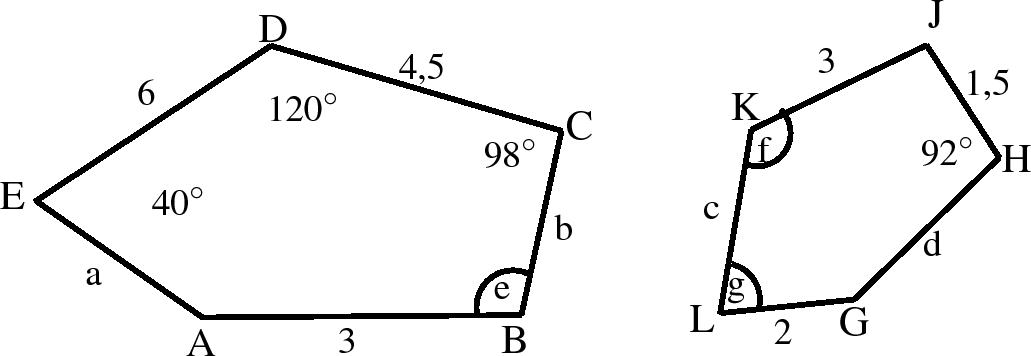
\includegraphics[width=300px]{col11306.imgs/m39354_MG10C14_012.png} % m39354;MG10C14\_012.png;;;6.0;8.5;
        
      \vspace{2pt}
    \vspace{.1in}
    
    \end{center}

 \end{figure}   

    \addtocounter{footnote}{-0}
    
        \par 
        
        \vspace{5pt}
        \label{m39354*solfhsst!!!underscore!!!id745}\noindent\textbf{Solution to Exercise } \label{m39354*listfhsst!!!underscore!!!id745}\begin{enumerate}[noitemsep, label=\textbf{Step} \textbf{\arabic*}. ] 
            \leftskip=20pt\rightskip=\leftskip\item  
        \label{m39354*id65725}We are given that ABCDE and GHJKL are similar. This means that:\par 
        \label{m39354*id65729}\nopagebreak\noindent{}
          \settowidth{\mymathboxwidth}{\begin{equation}
    \frac{\mathrm{AB}}{\mathrm{GH}}=\frac{\mathrm{BC}}{\mathrm{HJ}}=\frac{\mathrm{CD}}{\mathrm{JK}}=\frac{\mathrm{DE}}{\mathrm{KL}}=\frac{\mathrm{EA}}{\mathrm{LG}}\tag{13.4}
      \end{equation}
    }
    \typeout{Columnwidth = \the\columnwidth}\typeout{math as usual width = \the\mymathboxwidth}
    \ifthenelse{\lengthtest{\mymathboxwidth < \columnwidth}}{% if the math fits, do it again, for real
    \begin{equation}
    \frac{\mathrm{AB}}{\mathrm{GH}}=\frac{\mathrm{BC}}{\mathrm{HJ}}=\frac{\mathrm{CD}}{\mathrm{JK}}=\frac{\mathrm{DE}}{\mathrm{KL}}=\frac{\mathrm{EA}}{\mathrm{LG}}\tag{13.4}
      \end{equation}
    }{% else, if it doesn't fit
    \setlength{\mymathboxwidth}{\columnwidth}
      \addtolength{\mymathboxwidth}{-48pt}
    \par\vspace{12pt}\noindent\begin{minipage}{\columnwidth}
    \parbox[t]{\mymathboxwidth}{\large\begin{math}
    \frac{\mathrm{AB}}{\mathrm{GH}}=\frac{\mathrm{BC}}{\mathrm{HJ}}=\frac{\mathrm{CD}}{\mathrm{JK}}=\frac{\mathrm{DE}}{\mathrm{KL}}=\frac{\mathrm{EA}}{\mathrm{LG}}\end{math}}\hfill
    \parbox[t]{48pt}{\raggedleft 
    (13.4)}
    \end{minipage}\vspace{12pt}\par
    }% end of conditional for this bit of math
    \typeout{math as usual width = \the\mymathboxwidth}
    
        
        \label{m39354*id65782}and\par 
        \label{m39354*id65787}\nopagebreak\noindent{}
          \settowidth{\mymathboxwidth}{\begin{equation}
    \begin{array}{ccc}\hfill \hat{A}& =& \hat{G}\hfill \\ \hfill \hat{B}& =& \hat{H}\hfill \\ \hfill \hat{C}& =& \hat{J}\hfill \\ \hfill \hat{D}& =& \hat{K}\hfill \\ \hfill \hat{E}& =& \hat{L}\hfill \end{array}\tag{13.5}
      \end{equation}
    }
    \typeout{Columnwidth = \the\columnwidth}\typeout{math as usual width = \the\mymathboxwidth}
    \ifthenelse{\lengthtest{\mymathboxwidth < \columnwidth}}{% if the math fits, do it again, for real
    \begin{equation}
    \begin{array}{ccc}\hfill \hat{A}& =& \hat{G}\hfill \\ \hfill \hat{B}& =& \hat{H}\hfill \\ \hfill \hat{C}& =& \hat{J}\hfill \\ \hfill \hat{D}& =& \hat{K}\hfill \\ \hfill \hat{E}& =& \hat{L}\hfill \end{array}\tag{13.5}
      \end{equation}
    }{% else, if it doesn't fit
    \setlength{\mymathboxwidth}{\columnwidth}
      \addtolength{\mymathboxwidth}{-48pt}
    \par\vspace{12pt}\noindent\begin{minipage}{\columnwidth}
    \parbox[t]{\mymathboxwidth}{\large\begin{math}
    \hat{A}=\hat{G}\hat{B}=\hat{H}\hat{C}=\hat{J}\hat{D}=\hat{K}\hat{E}=\hat{L}\end{math}}\hfill
    \parbox[t]{48pt}{\raggedleft 
    (13.5)}
    \end{minipage}\vspace{12pt}\par
    }% end of conditional for this bit of math
    \typeout{math as usual width = \the\mymathboxwidth}
    
        
        \item  
        \label{m39354*id65948}We are required to determine the\par 
        \label{m39354*id65951}\begin{enumerate}[noitemsep, label=\textbf{\alph*}. ] 
            \leftskip=20pt\rightskip=\leftskip\label{m39354*uid32}\item \begin{math}a\end{math}, \begin{math}b\end{math}, \begin{math}c\end{math} and \begin{math}d\end{math}, and
\label{m39354*uid33}\item \begin{math}e\end{math}, \begin{math}f\end{math} and \begin{math}g\end{math}.
\end{enumerate}
        
        \item  
        \label{m39354*id66048}The corresponding angles are equal, so no calculation is needed. We are given one pair of sides \begin{math}DC\end{math} and \begin{math}KJ\end{math} that correspond. \begin{math}\frac{DC}{KJ}=\frac{4,5}{3}=1,5\end{math} so we know that all sides of \begin{math}KJHGL\end{math} are 1,5 times smaller than \begin{math}ABCDE\end{math}.\par 
        \item  
        \label{m39354*id66160}\nopagebreak\noindent{}
          \settowidth{\mymathboxwidth}{\begin{equation}
    \begin{array}{ccc}\hfill \frac{a}{2}=1,5& \therefore & a=2\ensuremath{\times}1,5=3\hfill \\ \hfill \frac{b}{1,5}=1,5& \therefore & b=1,5\ensuremath{\times}1,5=2,25\hfill \\ \hfill \frac{6}{c}=1,5& \therefore & c=6÷1,5=4\hfill \\ \hfill d=\frac{3}{1,5}& \therefore & d=2\hfill \end{array}\tag{13.6}
      \end{equation}
    }
    \typeout{Columnwidth = \the\columnwidth}\typeout{math as usual width = \the\mymathboxwidth}
    \ifthenelse{\lengthtest{\mymathboxwidth < \columnwidth}}{% if the math fits, do it again, for real
    \begin{equation}
    \begin{array}{ccc}\hfill \frac{a}{2}=1,5& \therefore & a=2\ensuremath{\times}1,5=3\hfill \\ \hfill \frac{b}{1,5}=1,5& \therefore & b=1,5\ensuremath{\times}1,5=2,25\hfill \\ \hfill \frac{6}{c}=1,5& \therefore & c=6÷1,5=4\hfill \\ \hfill d=\frac{3}{1,5}& \therefore & d=2\hfill \end{array}\tag{13.6}
      \end{equation}
    }{% else, if it doesn't fit
    \setlength{\mymathboxwidth}{\columnwidth}
      \addtolength{\mymathboxwidth}{-48pt}
    \par\vspace{12pt}\noindent\begin{minipage}{\columnwidth}
    \parbox[t]{\mymathboxwidth}{\large\begin{math}
    \frac{a}{2}=1,5\therefore a=2\ensuremath{\times}1,5=3\frac{b}{1,5}=1,5\therefore b=1,5\ensuremath{\times}1,5=2,25\frac{6}{c}=1,5\therefore c=6÷1,5=4d=\frac{3}{1,5}\therefore d=2\end{math}}\hfill
    \parbox[t]{48pt}{\raggedleft 
    (13.6)}
    \end{minipage}\vspace{12pt}\par
    }% end of conditional for this bit of math
    \typeout{math as usual width = \the\mymathboxwidth}
    
        
        \item  
        \label{m39354*id66368}\nopagebreak\noindent{}\settowidth{\mymathboxwidth}{\begin{equation}
    \begin{array}{ccc}\hfill e& =& {92}^{\circ }\left(\mathrm{corresponds\; to\; H}\right)\hfill \\ \hfill f& =& {120}^{\circ }\left(\mathrm{corresponds\; to\; D}\right)\hfill \\ \hfill g& =& {40}^{\circ }\left(\mathrm{corresponds\; to\; E}\right)\hfill \end{array}\tag{13.7}
      \end{equation}
    }
    \typeout{Columnwidth = \the\columnwidth}\typeout{math as usual width = \the\mymathboxwidth}
    \ifthenelse{\lengthtest{\mymathboxwidth < \columnwidth}}{% if the math fits, do it again, for real
    \begin{equation}
    \begin{array}{ccc}\hfill e& =& {92}^{\circ }\left(\mathrm{corresponds\; to\; H}\right)\hfill \\ \hfill f& =& {120}^{\circ }\left(\mathrm{corresponds\; to\; D}\right)\hfill \\ \hfill g& =& {40}^{\circ }\left(\mathrm{corresponds\; to\; E}\right)\hfill \end{array}\tag{13.7}
      \end{equation}
    }{% else, if it doesn't fit
    \setlength{\mymathboxwidth}{\columnwidth}
      \addtolength{\mymathboxwidth}{-48pt}
    \par\vspace{12pt}\noindent\begin{minipage}{\columnwidth}
    \parbox[t]{\mymathboxwidth}{\large\begin{math}
    e={92}^{\circ }\left(\mathrm{corresponds\; to\; H}\right)f={120}^{\circ }\left(\mathrm{corresponds\; to\; D}\right)g={40}^{\circ }\left(\mathrm{corresponds\; to\; E}\right)\end{math}}\hfill
    \parbox[t]{48pt}{\raggedleft 
    (13.7)}
    \end{minipage}\vspace{12pt}\par
    }% end of conditional for this bit of math
    \typeout{math as usual width = \the\mymathboxwidth}
    
        
        \item  
        \label{m39354*id66506}\nopagebreak\noindent{}
          \settowidth{\mymathboxwidth}{\begin{equation}
    \begin{array}{ccc}\hfill a& =& 3\hfill \\ \hfill b& =& 2,25\hfill \\ \hfill c& =& 4\hfill \\ \hfill d& =& 2\hfill \\ \hfill e& =& {92}^{\circ }\hfill \\ \hfill f& =& {120}^{\circ }\hfill \\ \hfill g& =& {40}^{\circ }\hfill \end{array}\tag{13.8}
      \end{equation}
    }
    \typeout{Columnwidth = \the\columnwidth}\typeout{math as usual width = \the\mymathboxwidth}
    \ifthenelse{\lengthtest{\mymathboxwidth < \columnwidth}}{% if the math fits, do it again, for real
    \begin{equation}
    \begin{array}{ccc}\hfill a& =& 3\hfill \\ \hfill b& =& 2,25\hfill \\ \hfill c& =& 4\hfill \\ \hfill d& =& 2\hfill \\ \hfill e& =& {92}^{\circ }\hfill \\ \hfill f& =& {120}^{\circ }\hfill \\ \hfill g& =& {40}^{\circ }\hfill \end{array}\tag{13.8}
      \end{equation}
    }{% else, if it doesn't fit
    \setlength{\mymathboxwidth}{\columnwidth}
      \addtolength{\mymathboxwidth}{-48pt}
    \par\vspace{12pt}\noindent\begin{minipage}{\columnwidth}
    \parbox[t]{\mymathboxwidth}{\large\begin{math}
    a=3b=2,25c=4d=2e={92}^{\circ }f={120}^{\circ }g={40}^{\circ }\end{math}}\hfill
    \parbox[t]{48pt}{\raggedleft 
    (13.8)}
    \end{minipage}\vspace{12pt}\par
    }% end of conditional for this bit of math
    \typeout{math as usual width = \the\mymathboxwidth}
    
        
        
        \end{enumerate}
         

    \end{exercise}
    \end{mdframed}
    }
    \noindent
  
\label{m39354*secfhsst!!!underscore!!!id1187}
            \subsubsection{ Activity: Similarity of Equilateral Triangles }
            \nopagebreak
            
\label{m39354*uid34283409} Working in pairs, show that all equilateral triangles are similar. \par 
        

\label{m39354*secfhsst!!!underscore!!!id1190}
            \subsubsection{  Polygons-mixed }
            \nopagebreak
            
        \label{m39354*id66690}\begin{enumerate}[noitemsep, label=\textbf{\arabic*}. ] 
            \label{m39354*uid34}\item Find the values of the unknowns in each case. Give reasons.

    \setcounter{subfigure}{0}


	\begin{figure}[H] % horizontal\label{m39354*id66710}
    \begin{center}
    \label{m39354*id66710!!!underscore!!!media}\label{m39354*id66710!!!underscore!!!printimage}\includegraphics{col11306.imgs/m39354_mg10c14_2.png} % m39354;mg10c14\_2.png;;;6.0;8.5;
        
      \vspace{2pt}
    \vspace{.1in}
    
    \end{center}

 \end{figure}   

    \addtocounter{footnote}{-0}
            \label{m39354*uid35}\item 
Find the angles and lengths marked with letters in the following figures:

    \setcounter{subfigure}{0}


	\begin{figure}[H] % horizontal\label{m39354*id66733}
    \begin{center}
    \label{m39354*id66733!!!underscore!!!media}\label{m39354*id66733!!!underscore!!!printimage}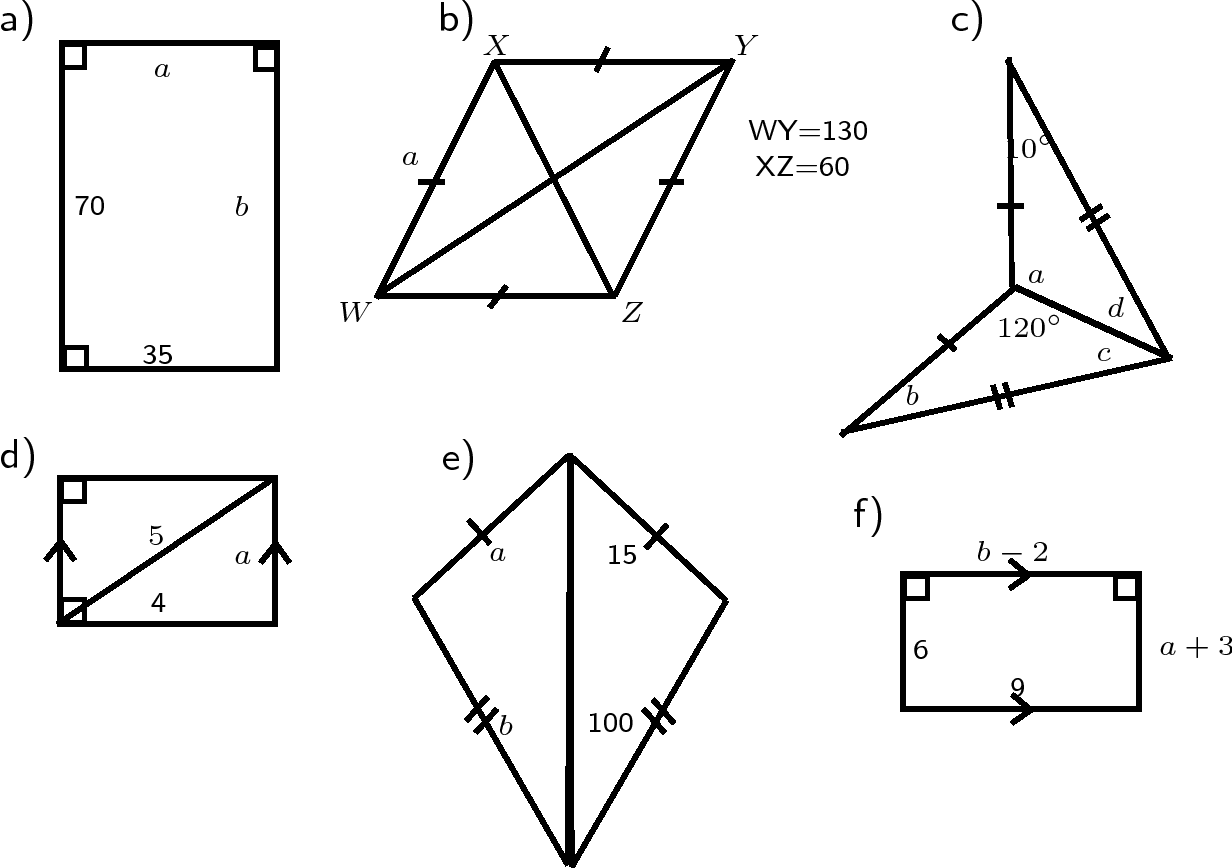
\includegraphics[width=300px]{col11306.imgs/m39354_MG10C14_014.png} % m39354;MG10C14\_014.png;;;6.0;8.5;
        
      \vspace{2pt}
    \vspace{.1in}
    
    \end{center}

 \end{figure}   

    \addtocounter{footnote}{-0}
            \end{enumerate}
        
        

      
    
      \label{m39354*eip-824}
\par \raisebox{-5 pt}{
\includegraphics[width=0.5cm]{col11306.imgs/summary_www.png}} Find the answers with the shortcodes:
 \par \begin{tabular}[h]{cccccc}
 (1.) liD  &  (2.) liW  & \end{tabular}



            \subsection{ Investigation: Defining polygons}
            \nopagebreak
            \label{m39354*eip-779}Investigate the different ways of defining polygons. Polygons that you should pay special attention to are: \label{m39354*id6342}\begin{itemize}[noitemsep]
            \item Isoceles, equilateral and right-angled triangle\item Kites, parallelograms, rectangles, rhombuses (or 'rhombi'), squares and trapeziums\end{itemize}
        
\par 
\label{m39354*id7342}
Things to consider are how these figures have been defined in this book and what alternative definitions exist. For example, a triangle is a three-sided polygon or a figure having three sides and three angles. Triangles can be classified using either their sides or their angles. Could you also classify quadrilaterals in this way? What other names exist for these figures? For example, quadrilaterals can also be called tetragons.
\par 

  \label{m39354**end}
          
         \section{ Proofs and conjectures}
    \nopagebreak
            \label{m39352} $ \hspace{-5pt}\begin{array}{cccccccccccc}   
\includegraphics[width=0.75cm]{col11306.imgs/summary_fullmarks.png} &   \end{array} $ \hspace{2 pt}\raisebox{-5 pt}{} {(section shortcode: MG10094 )} \par 
    
    
    
    
    
    
  
\label{m39352*secfhsst!!!underscore!!!id933}
            \subsection{ Proofs and conjectures in geometry}
            \nopagebreak
            \label{m39352*id0723}You have seen how to use geometry and the properties of polygons to help you find unknown lengths and angles in various quadrilaterals and polygons. We will now extend this work to proving some of the properties and to solving riders. A conjecture is the mathematicians way of saying I believe that this is true, but I have no proof. The following worked examples will help make this clearer. 
\par 
\label{m39352*probfhsst!!!underscore!!!id072}\vspace{.5cm} 
      
      \noindent
      \hspace*{-30pt}
\includegraphics[width=0.5in]{col11306.imgs/pspencil2.png}   \raisebox{25mm}{   
      \begin{mdframed}[linewidth=4, leftmargin=40, rightmargin=40]  
      \begin{exercise}
    \noindent\textbf{Exercise 13.3: Proofs - 1}\label{m39352*id97832}\label{m39352*id943}Given quadrilateral ABCD, with \begin{math}AB\parallel CD\end{math} and \begin{math}AD\parallel BC\end{math}, prove that \begin{math}B\hat{A}D=B\hat{C}A\end{math} and \begin{math}A\hat{B}C=A\hat{D}C\end{math}.\par 
\vspace{5pt}
\label{m39352*solfhsst!!!underscore!!!id083}\noindent\textbf{Solution to Exercise }\label{m39352*id08324}\begin{enumerate}[noitemsep, label=\textbf{Step} \textbf{\arabic*}. ] 
            \leftskip=20pt\rightskip=\leftskip\item We draw the following diagram and construct the diagonals.

    \setcounter{subfigure}{0}


	\begin{figure}[H] % horizontal\label{m39352*uid310}
    \begin{center}
    \label{m39352*id897}\label{m39352*uid310!!!underscore!!!printimage}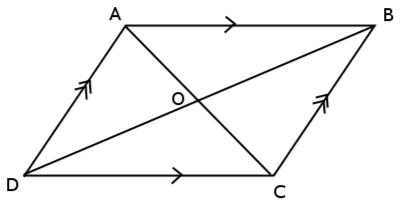
\includegraphics{col11306.imgs/m39352_geomproof1.png} % ;geomproof1.png;;;6.0;8.5;
        
      \vspace{2pt}
    \vspace{.1in}
    
    \end{center}

 \end{figure}   

    \addtocounter{footnote}{-0}
    
\item Given: \begin{math}AB\parallel CD\end{math} and \begin{math}AD\parallel BC\end{math}. We need to prove \begin{math}A=C\end{math} and \begin{math}B=D\end{math}. In the formal language of maths we say that we are required to prove (RTP) \begin{math}B\hat{A}D=B\hat{C}A\end{math} and \begin{math}A\hat{B}C=A\hat{D}C\end{math}. \item \label{m39352*id3468}\nopagebreak\noindent{}\settowidth{\mymathboxwidth}{\begin{equation}
    \begin{array}{cccc}\hfill B\hat{A}C& =& A\hat{C}D\hfill & \left(\mathrm{corresponding\; angles}\right)\\ \hfill D\hat{A}C& =& B\hat{C}A\hfill & \left(\mathrm{corresponding\; angles}\right)\\ \hfill B\hat{A}D& =& B\hat{C}A\hfill & \end{array}\tag{13.9}
      \end{equation}
    }
    \typeout{Columnwidth = \the\columnwidth}\typeout{math as usual width = \the\mymathboxwidth}
    \ifthenelse{\lengthtest{\mymathboxwidth < \columnwidth}}{% if the math fits, do it again, for real
    \begin{equation}
    \begin{array}{cccc}\hfill B\hat{A}C& =& A\hat{C}D\hfill & \left(\mathrm{corresponding\; angles}\right)\\ \hfill D\hat{A}C& =& B\hat{C}A\hfill & \left(\mathrm{corresponding\; angles}\right)\\ \hfill B\hat{A}D& =& B\hat{C}A\hfill & \end{array}\tag{13.9}
      \end{equation}
    }{% else, if it doesn't fit
    \setlength{\mymathboxwidth}{\columnwidth}
      \addtolength{\mymathboxwidth}{-48pt}
    \par\vspace{12pt}\noindent\begin{minipage}{\columnwidth}
    \parbox[t]{\mymathboxwidth}{\large\begin{math}
    B\hat{A}C=A\hat{C}D\left(\mathrm{corresponding\; angles}\right)D\hat{A}C=B\hat{C}A\left(\mathrm{corresponding\; angles}\right)B\hat{A}D=B\hat{C}A\end{math}}\hfill
    \parbox[t]{48pt}{\raggedleft 
    (13.9)}
    \end{minipage}\vspace{12pt}\par
    }% end of conditional for this bit of math
    \typeout{math as usual width = \the\mymathboxwidth}
    
        
Similarly we find that: 
\label{m39352*id97}\nopagebreak\noindent{}\settowidth{\mymathboxwidth}{\begin{equation}
    A\hat{B}C=A\hat{D}C\tag{13.10}
      \end{equation}
    }
    \typeout{Columnwidth = \the\columnwidth}\typeout{math as usual width = \the\mymathboxwidth}
    \ifthenelse{\lengthtest{\mymathboxwidth < \columnwidth}}{% if the math fits, do it again, for real
    \begin{equation}
    A\hat{B}C=A\hat{D}C\tag{13.10}
      \end{equation}
    }{% else, if it doesn't fit
    \setlength{\mymathboxwidth}{\columnwidth}
      \addtolength{\mymathboxwidth}{-48pt}
    \par\vspace{12pt}\noindent\begin{minipage}{\columnwidth}
    \parbox[t]{\mymathboxwidth}{\large\begin{math}
    A\hat{B}C=A\hat{D}C\end{math}}\hfill
    \parbox[t]{48pt}{\raggedleft 
    (13.10)}
    \end{minipage}\vspace{12pt}\par
    }% end of conditional for this bit of math
    \typeout{math as usual width = \the\mymathboxwidth}
    
\end{enumerate}
        


    \end{exercise}
    \end{mdframed}
    }
    \noindent
  

\par
            \label{m39352*probfhsst!!!underscore!!!id073}\vspace{.5cm} 
      
      \noindent
      \hspace*{-30pt}
\includegraphics[width=0.5in]{col11306.imgs/pspencil2.png}   \raisebox{25mm}{   
      \begin{mdframed}[linewidth=4, leftmargin=40, rightmargin=40]  
      \begin{exercise}
    \noindent\textbf{Proofs - 2 13.4}
\label{m39352*id973452}\label{m39352*id95433}In parallelogram ABCD, the bisectors of the angles (AW, BX, CY and DZ) have been constructed:

    \setcounter{subfigure}{0}


	\begin{figure}[H] % horizontal\label{m39352*uid4140}
    \begin{center}
    \label{m39352*uid4140!!!underscore!!!media}\label{m39352*uid4140!!!underscore!!!printimage}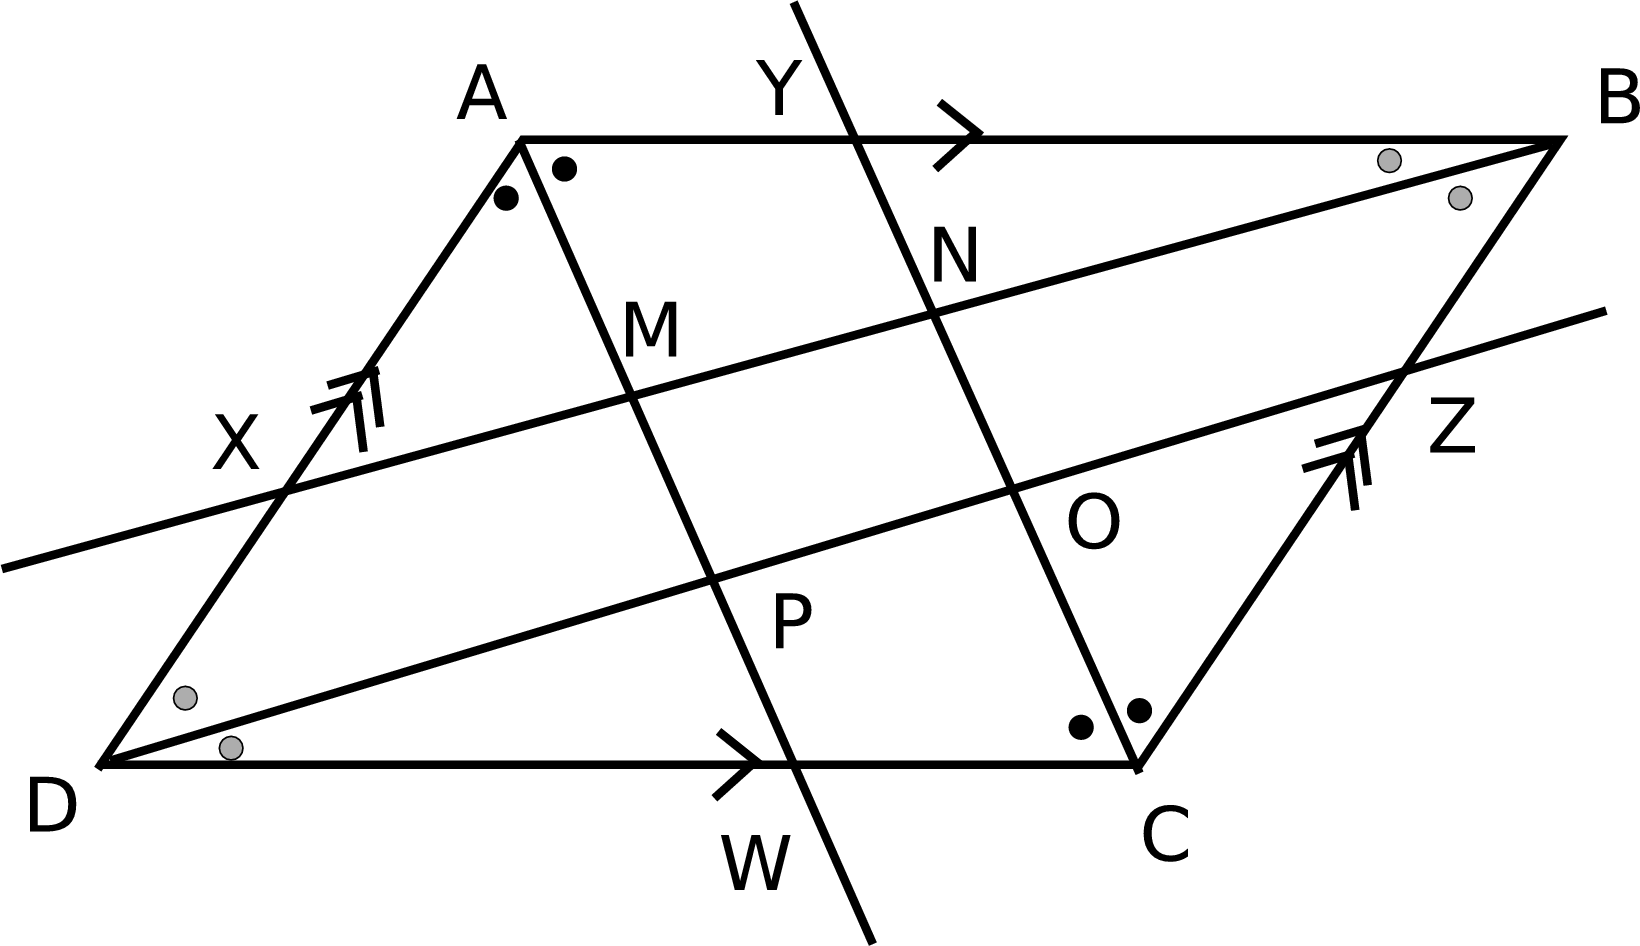
\includegraphics[width=300px]{col11306.imgs/m39352_geomproof2.png} % m39352;geomproof2.png;;;6.0;8.5;
        
      \vspace{2pt}
    \vspace{.1in}
    
    \end{center}

 \end{figure}   

    \addtocounter{footnote}{-0}
    
You are also given that \begin{math}\mathrm{AB}=\mathrm{CD}\end{math}, \begin{math}\mathrm{AD}=\mathrm{BC}\end{math}, \begin{math}\mathrm{AB}\parallel \mathrm{CD}\end{math}, \begin{math}\mathrm{AD}\parallel \mathrm{BC}\end{math},  \begin{math}\hat{A}=\hat{C}\end{math}, and \begin{math}\hat{B}=\hat{D}\end{math}. 
Prove that MNOP is a parallelogram.\par 
\vspace{5pt}
\label{m39352*solfhsst!!!underscore!!!id023}\noindent\textbf{Solution to Exercise }\label{m39352*id085424}\begin{enumerate}[noitemsep, label=\textbf{Step} \textbf{\arabic*}. ] 
            \leftskip=20pt\rightskip=\leftskip\item Given: \begin{math}\mathrm{AB}=\mathrm{CD}\end{math}, \begin{math}\mathrm{AD}=\mathrm{BC}\end{math}, \begin{math}\mathrm{AB}\parallel \mathrm{CD}\end{math}, \begin{math}\mathrm{AD}\parallel \mathrm{BC}\end{math},  \begin{math}\hat{A}=\hat{C}\end{math}, and \begin{math}\hat{B}=\hat{D}\end{math}. RTP: MNOP is a parallelogram.\item 




\label{m39352*id368}\nopagebreak\noindent{}\settowidth{\mymathboxwidth}{\begin{equation}
    \begin{array}{cc}\hfill In\phantom{\rule{2pt}{0ex}}▵\phantom{\rule{2pt}{0ex}}\mathrm{ADW}\phantom{\rule{2pt}{0ex}}\mathrm{and}\phantom{\rule{2pt}{0ex}}▵\mathrm{CBY}\phantom{\rule{2pt}{0ex}}\\ \hfill D\hat{A}W& =& B\hat{C}Y\phantom{\rule{2pt}{0ex}}\left(\mathrm{given}\right)\hfill \\ \hfill A\hat{D}C& =& A\hat{B}C\phantom{\rule{2pt}{0ex}}\left(\mathrm{given}\right)\hfill \\ \hfill \mathrm{AD}& =& \mathrm{BC}\phantom{\rule{2pt}{0ex}}\mathrm{\left(given\right)}\hfill \\ \hfill \therefore \phantom{\rule{2pt}{0ex}}▵\mathrm{ADW}& =& ▵\mathrm{CBY}\phantom{\rule{2pt}{0ex}}\mathrm{\left(AAS\right)}\hfill \\ \hfill \therefore \phantom{\rule{2pt}{0ex}}\mathrm{DW}& =& \mathrm{BY}\hfill \end{array}\tag{13.11}
      \end{equation}
    }
    \typeout{Columnwidth = \the\columnwidth}\typeout{math as usual width = \the\mymathboxwidth}
    \ifthenelse{\lengthtest{\mymathboxwidth < \columnwidth}}{% if the math fits, do it again, for real
    \begin{equation}
    \begin{array}{cc}\hfill In\phantom{\rule{2pt}{0ex}}▵\phantom{\rule{2pt}{0ex}}\mathrm{ADW}\phantom{\rule{2pt}{0ex}}\mathrm{and}\phantom{\rule{2pt}{0ex}}▵\mathrm{CBY}\phantom{\rule{2pt}{0ex}}\\ \hfill D\hat{A}W& =& B\hat{C}Y\phantom{\rule{2pt}{0ex}}\left(\mathrm{given}\right)\hfill \\ \hfill A\hat{D}C& =& A\hat{B}C\phantom{\rule{2pt}{0ex}}\left(\mathrm{given}\right)\hfill \\ \hfill \mathrm{AD}& =& \mathrm{BC}\phantom{\rule{2pt}{0ex}}\mathrm{\left(given\right)}\hfill \\ \hfill \therefore \phantom{\rule{2pt}{0ex}}▵\mathrm{ADW}& =& ▵\mathrm{CBY}\phantom{\rule{2pt}{0ex}}\mathrm{\left(AAS\right)}\hfill \\ \hfill \therefore \phantom{\rule{2pt}{0ex}}\mathrm{DW}& =& \mathrm{BY}\hfill \end{array}\tag{13.11}
      \end{equation}
    }{% else, if it doesn't fit
    \setlength{\mymathboxwidth}{\columnwidth}
      \addtolength{\mymathboxwidth}{-48pt}
    \par\vspace{12pt}\noindent\begin{minipage}{\columnwidth}
    \parbox[t]{\mymathboxwidth}{\large\begin{math}
    In\phantom{\rule{2pt}{0ex}}▵\phantom{\rule{2pt}{0ex}}\mathrm{ADW}\phantom{\rule{2pt}{0ex}}\mathrm{and}\phantom{\rule{2pt}{0ex}}▵\mathrm{CBY}\phantom{\rule{2pt}{0ex}}D\hat{A}W=B\hat{C}Y\phantom{\rule{2pt}{0ex}}\left(\mathrm{given}\right)A\hat{D}C=A\hat{B}C\phantom{\rule{2pt}{0ex}}\left(\mathrm{given}\right)\mathrm{AD}=\mathrm{BC}\phantom{\rule{2pt}{0ex}}\mathrm{\left(given\right)}\therefore \phantom{\rule{2pt}{0ex}}▵\mathrm{ADW}=▵\mathrm{CBY}\phantom{\rule{2pt}{0ex}}\mathrm{\left(AAS\right)}\therefore \phantom{\rule{2pt}{0ex}}\mathrm{DW}=\mathrm{BY}\end{math}}\hfill
    \parbox[t]{48pt}{\raggedleft 
    (13.11)}
    \end{minipage}\vspace{12pt}\par
    }% end of conditional for this bit of math
    \typeout{math as usual width = \the\mymathboxwidth}
    
        
\label{m39352*id378}\nopagebreak\noindent{}\settowidth{\mymathboxwidth}{\begin{equation}
    \begin{array}{cc}\hfill In\phantom{\rule{2pt}{0ex}}▵\phantom{\rule{2pt}{0ex}}\mathrm{ABX}\phantom{\rule{2pt}{0ex}}\mathrm{and}\phantom{\rule{2pt}{0ex}}▵\mathrm{CDZ}\phantom{\rule{2pt}{0ex}}\\ \hfill D\hat{C}Z& =& B\hat{A}X\phantom{\rule{2pt}{0ex}}\left(\mathrm{given}\right)\hfill \\ \hfill Z\hat{D}C& =& X\hat{B}A\phantom{\rule{2pt}{0ex}}\left(\mathrm{given}\right)\hfill \\ \hfill \mathrm{DC}& =& \mathrm{AB}\phantom{\rule{2pt}{0ex}}\mathrm{\left(given\right)}\hfill \\ \hfill \therefore \phantom{\rule{2pt}{0ex}}▵\mathrm{ABX}& \equiv & ▵\mathrm{CDZ}\phantom{\rule{2pt}{0ex}}\mathrm{\left(AAS\right)}\hfill \\ \hfill \therefore \phantom{\rule{2pt}{0ex}}\mathrm{AX}& =& \mathrm{CZ}\hfill \end{array}\tag{13.12}
      \end{equation}
    }
    \typeout{Columnwidth = \the\columnwidth}\typeout{math as usual width = \the\mymathboxwidth}
    \ifthenelse{\lengthtest{\mymathboxwidth < \columnwidth}}{% if the math fits, do it again, for real
    \begin{equation}
    \begin{array}{cc}\hfill In\phantom{\rule{2pt}{0ex}}▵\phantom{\rule{2pt}{0ex}}\mathrm{ABX}\phantom{\rule{2pt}{0ex}}\mathrm{and}\phantom{\rule{2pt}{0ex}}▵\mathrm{CDZ}\phantom{\rule{2pt}{0ex}}\\ \hfill D\hat{C}Z& =& B\hat{A}X\phantom{\rule{2pt}{0ex}}\left(\mathrm{given}\right)\hfill \\ \hfill Z\hat{D}C& =& X\hat{B}A\phantom{\rule{2pt}{0ex}}\left(\mathrm{given}\right)\hfill \\ \hfill \mathrm{DC}& =& \mathrm{AB}\phantom{\rule{2pt}{0ex}}\mathrm{\left(given\right)}\hfill \\ \hfill \therefore \phantom{\rule{2pt}{0ex}}▵\mathrm{ABX}& \equiv & ▵\mathrm{CDZ}\phantom{\rule{2pt}{0ex}}\mathrm{\left(AAS\right)}\hfill \\ \hfill \therefore \phantom{\rule{2pt}{0ex}}\mathrm{AX}& =& \mathrm{CZ}\hfill \end{array}\tag{13.12}
      \end{equation}
    }{% else, if it doesn't fit
    \setlength{\mymathboxwidth}{\columnwidth}
      \addtolength{\mymathboxwidth}{-48pt}
    \par\vspace{12pt}\noindent\begin{minipage}{\columnwidth}
    \parbox[t]{\mymathboxwidth}{\large\begin{math}
    In\phantom{\rule{2pt}{0ex}}▵\phantom{\rule{2pt}{0ex}}\mathrm{ABX}\phantom{\rule{2pt}{0ex}}\mathrm{and}\phantom{\rule{2pt}{0ex}}▵\mathrm{CDZ}\phantom{\rule{2pt}{0ex}}D\hat{C}Z=B\hat{A}X\phantom{\rule{2pt}{0ex}}\left(\mathrm{given}\right)Z\hat{D}C=X\hat{B}A\phantom{\rule{2pt}{0ex}}\left(\mathrm{given}\right)\mathrm{DC}=\mathrm{AB}\phantom{\rule{2pt}{0ex}}\mathrm{\left(given\right)}\therefore \phantom{\rule{2pt}{0ex}}▵\mathrm{ABX}\equiv ▵\mathrm{CDZ}\phantom{\rule{2pt}{0ex}}\mathrm{\left(AAS\right)}\therefore \phantom{\rule{2pt}{0ex}}\mathrm{AX}=\mathrm{CZ}\end{math}}\hfill
    \parbox[t]{48pt}{\raggedleft 
    (13.12)}
    \end{minipage}\vspace{12pt}\par
    }% end of conditional for this bit of math
    \typeout{math as usual width = \the\mymathboxwidth}
    
        

\label{m39352*id38868}\nopagebreak\noindent{}\settowidth{\mymathboxwidth}{\begin{equation}
    \begin{array}{cc}\hfill In\phantom{\rule{2pt}{0ex}}▵\phantom{\rule{2pt}{0ex}}\mathrm{XAM}\phantom{\rule{2pt}{0ex}}\mathrm{and}\phantom{\rule{2pt}{0ex}}▵\mathrm{ZCO}\phantom{\rule{2pt}{0ex}}\\ \hfill X\hat{A}M& =& Z\hat{C}O\phantom{\rule{2pt}{0ex}}\left(\mathrm{given}\right)\hfill \\ \hfill A\hat{X}M& =& C\hat{Z}O\phantom{\rule{2pt}{0ex}}\left(\mathrm{proven\; above}\right)\hfill \\ \hfill \mathrm{AX}& =& \mathrm{CZ}\phantom{\rule{2pt}{0ex}}\mathrm{\left(proven\; above\right)}\hfill \\ \hfill \therefore \phantom{\rule{2pt}{0ex}}▵\mathrm{XAM}& \equiv & ▵\mathrm{COZ}\phantom{\rule{2pt}{0ex}}\mathrm{\left(AAS\right)}\hfill \\ \hfill \therefore \phantom{\rule{2pt}{0ex}}A\hat{O}C& =& A\hat{M}X\hfill \end{array}\tag{13.13}
      \end{equation}
    }
    \typeout{Columnwidth = \the\columnwidth}\typeout{math as usual width = \the\mymathboxwidth}
    \ifthenelse{\lengthtest{\mymathboxwidth < \columnwidth}}{% if the math fits, do it again, for real
    \begin{equation}
    \begin{array}{cc}\hfill In\phantom{\rule{2pt}{0ex}}▵\phantom{\rule{2pt}{0ex}}\mathrm{XAM}\phantom{\rule{2pt}{0ex}}\mathrm{and}\phantom{\rule{2pt}{0ex}}▵\mathrm{ZCO}\phantom{\rule{2pt}{0ex}}\\ \hfill X\hat{A}M& =& Z\hat{C}O\phantom{\rule{2pt}{0ex}}\left(\mathrm{given}\right)\hfill \\ \hfill A\hat{X}M& =& C\hat{Z}O\phantom{\rule{2pt}{0ex}}\left(\mathrm{proven\; above}\right)\hfill \\ \hfill \mathrm{AX}& =& \mathrm{CZ}\phantom{\rule{2pt}{0ex}}\mathrm{\left(proven\; above\right)}\hfill \\ \hfill \therefore \phantom{\rule{2pt}{0ex}}▵\mathrm{XAM}& \equiv & ▵\mathrm{COZ}\phantom{\rule{2pt}{0ex}}\mathrm{\left(AAS\right)}\hfill \\ \hfill \therefore \phantom{\rule{2pt}{0ex}}A\hat{O}C& =& A\hat{M}X\hfill \end{array}\tag{13.13}
      \end{equation}
    }{% else, if it doesn't fit
    \setlength{\mymathboxwidth}{\columnwidth}
      \addtolength{\mymathboxwidth}{-48pt}
    \par\vspace{12pt}\noindent\begin{minipage}{\columnwidth}
    \parbox[t]{\mymathboxwidth}{\large\begin{math}
    In\phantom{\rule{2pt}{0ex}}▵\phantom{\rule{2pt}{0ex}}\mathrm{XAM}\phantom{\rule{2pt}{0ex}}\mathrm{and}\phantom{\rule{2pt}{0ex}}▵\mathrm{ZCO}\phantom{\rule{2pt}{0ex}}X\hat{A}M=Z\hat{C}O\phantom{\rule{2pt}{0ex}}\left(\mathrm{given}\right)A\hat{X}M=C\hat{Z}O\phantom{\rule{2pt}{0ex}}\left(\mathrm{proven\; above}\right)\mathrm{AX}=\mathrm{CZ}\phantom{\rule{2pt}{0ex}}\mathrm{\left(proven\; above\right)}\therefore \phantom{\rule{2pt}{0ex}}▵\mathrm{XAM}\equiv ▵\mathrm{COZ}\phantom{\rule{2pt}{0ex}}\mathrm{\left(AAS\right)}\therefore \phantom{\rule{2pt}{0ex}}A\hat{O}C=A\hat{M}X\end{math}}\hfill
    \parbox[t]{48pt}{\raggedleft 
    (13.13)}
    \end{minipage}\vspace{12pt}\par
    }% end of conditional for this bit of math
    \typeout{math as usual width = \the\mymathboxwidth}
    
        

\label{m39352*eip-914}\nopagebreak\noindent{}\settowidth{\mymathboxwidth}{\begin{equation}
    \begin{array}{ccc}\hfill A\hat{M}X& =& P\hat{M}N\phantom{\rule{2pt}{0ex}}\mathrm{\left(vert.\; opp.\; \angle \text{'}s\right)}\hfill \\ \hfill C\hat{O}Z& =& N\hat{O}P\phantom{\rule{2pt}{0ex}}\mathrm{\left(vert.\; opp.\; \angle \text{'}s\right)}\hfill \\ \hfill \therefore \phantom{\rule{2pt}{0ex}}P\hat{M}N& =& N\hat{O}P\hfill \end{array}\tag{13.14}
      \end{equation}
    }
    \typeout{Columnwidth = \the\columnwidth}\typeout{math as usual width = \the\mymathboxwidth}
    \ifthenelse{\lengthtest{\mymathboxwidth < \columnwidth}}{% if the math fits, do it again, for real
    \begin{equation}
    \begin{array}{ccc}\hfill A\hat{M}X& =& P\hat{M}N\phantom{\rule{2pt}{0ex}}\mathrm{\left(vert.\; opp.\; \angle \text{'}s\right)}\hfill \\ \hfill C\hat{O}Z& =& N\hat{O}P\phantom{\rule{2pt}{0ex}}\mathrm{\left(vert.\; opp.\; \angle \text{'}s\right)}\hfill \\ \hfill \therefore \phantom{\rule{2pt}{0ex}}P\hat{M}N& =& N\hat{O}P\hfill \end{array}\tag{13.14}
      \end{equation}
    }{% else, if it doesn't fit
    \setlength{\mymathboxwidth}{\columnwidth}
      \addtolength{\mymathboxwidth}{-48pt}
    \par\vspace{12pt}\noindent\begin{minipage}{\columnwidth}
    \parbox[t]{\mymathboxwidth}{\large\begin{math}
    A\hat{M}X=P\hat{M}N\phantom{\rule{2pt}{0ex}}\mathrm{\left(vert.\; opp.\; \angle \text{'}s\right)}C\hat{O}Z=N\hat{O}P\phantom{\rule{2pt}{0ex}}\mathrm{\left(vert.\; opp.\; \angle \text{'}s\right)}\therefore \phantom{\rule{2pt}{0ex}}P\hat{M}N=N\hat{O}P\end{math}}\hfill
    \parbox[t]{48pt}{\raggedleft 
    (13.14)}
    \end{minipage}\vspace{12pt}\par
    }% end of conditional for this bit of math
    \typeout{math as usual width = \the\mymathboxwidth}
    \label{m39352*id3838}\nopagebreak\noindent{}\settowidth{\mymathboxwidth}{\begin{equation}
    \begin{array}{cc}\hfill In\phantom{\rule{2pt}{0ex}}▵\phantom{\rule{2pt}{0ex}}\mathrm{BYN}\phantom{\rule{2pt}{0ex}}\mathrm{and}\phantom{\rule{2pt}{0ex}}▵\mathrm{DWP}\phantom{\rule{2pt}{0ex}}\\ \hfill Y\hat{B}N& =& W\hat{D}P\phantom{\rule{2pt}{0ex}}\left(\mathrm{given}\right)\hfill \\ \hfill B\hat{Y}N& =& W\hat{D}P\phantom{\rule{2pt}{0ex}}\left(\mathrm{proven\; above}\right)\hfill \\ \hfill \mathrm{DW}& =& \mathrm{BY}\phantom{\rule{2pt}{0ex}}\mathrm{\left(proven\; above\right)}\hfill \\ \hfill \therefore \phantom{\rule{2pt}{0ex}}▵\mathrm{YBN}& \equiv & ▵\mathrm{WDP}\phantom{\rule{2pt}{0ex}}\mathrm{\left(AAS\right)}\hfill \\ \hfill \therefore \phantom{\rule{2pt}{0ex}}B\hat{N}Y& =& D\hat{P}W\hfill \end{array}\tag{13.15}
      \end{equation}
    }
    \typeout{Columnwidth = \the\columnwidth}\typeout{math as usual width = \the\mymathboxwidth}
    \ifthenelse{\lengthtest{\mymathboxwidth < \columnwidth}}{% if the math fits, do it again, for real
    \begin{equation}
    \begin{array}{cc}\hfill In\phantom{\rule{2pt}{0ex}}▵\phantom{\rule{2pt}{0ex}}\mathrm{BYN}\phantom{\rule{2pt}{0ex}}\mathrm{and}\phantom{\rule{2pt}{0ex}}▵\mathrm{DWP}\phantom{\rule{2pt}{0ex}}\\ \hfill Y\hat{B}N& =& W\hat{D}P\phantom{\rule{2pt}{0ex}}\left(\mathrm{given}\right)\hfill \\ \hfill B\hat{Y}N& =& W\hat{D}P\phantom{\rule{2pt}{0ex}}\left(\mathrm{proven\; above}\right)\hfill \\ \hfill \mathrm{DW}& =& \mathrm{BY}\phantom{\rule{2pt}{0ex}}\mathrm{\left(proven\; above\right)}\hfill \\ \hfill \therefore \phantom{\rule{2pt}{0ex}}▵\mathrm{YBN}& \equiv & ▵\mathrm{WDP}\phantom{\rule{2pt}{0ex}}\mathrm{\left(AAS\right)}\hfill \\ \hfill \therefore \phantom{\rule{2pt}{0ex}}B\hat{N}Y& =& D\hat{P}W\hfill \end{array}\tag{13.15}
      \end{equation}
    }{% else, if it doesn't fit
    \setlength{\mymathboxwidth}{\columnwidth}
      \addtolength{\mymathboxwidth}{-48pt}
    \par\vspace{12pt}\noindent\begin{minipage}{\columnwidth}
    \parbox[t]{\mymathboxwidth}{\large\begin{math}
    In\phantom{\rule{2pt}{0ex}}▵\phantom{\rule{2pt}{0ex}}\mathrm{BYN}\phantom{\rule{2pt}{0ex}}\mathrm{and}\phantom{\rule{2pt}{0ex}}▵\mathrm{DWP}\phantom{\rule{2pt}{0ex}}Y\hat{B}N=W\hat{D}P\phantom{\rule{2pt}{0ex}}\left(\mathrm{given}\right)B\hat{Y}N=W\hat{D}P\phantom{\rule{2pt}{0ex}}\left(\mathrm{proven\; above}\right)\mathrm{DW}=\mathrm{BY}\phantom{\rule{2pt}{0ex}}\mathrm{\left(proven\; above\right)}\therefore \phantom{\rule{2pt}{0ex}}▵\mathrm{YBN}\equiv ▵\mathrm{WDP}\phantom{\rule{2pt}{0ex}}\mathrm{\left(AAS\right)}\therefore \phantom{\rule{2pt}{0ex}}B\hat{N}Y=D\hat{P}W\end{math}}\hfill
    \parbox[t]{48pt}{\raggedleft 
    (13.15)}
    \end{minipage}\vspace{12pt}\par
    }% end of conditional for this bit of math
    \typeout{math as usual width = \the\mymathboxwidth}
    
        \label{m39352*eip-557}\nopagebreak\noindent{}\settowidth{\mymathboxwidth}{\begin{equation}
    \begin{array}{ccc}\hfill D\hat{P}W& =& M\hat{P}O\phantom{\rule{2pt}{0ex}}\mathrm{\left(vert.\; opp.\; \angle \text{'}s\right)}\hfill \\ \hfill B\hat{N}Y& =& O\hat{N}M\phantom{\rule{2pt}{0ex}}\mathrm{\left(vert.\; opp.\; \angle \text{'}s\right)}\hfill \\ \hfill \therefore \phantom{\rule{2pt}{0ex}}M\hat{P}O& =& O\hat{N}M\hfill \end{array}\tag{13.16}
      \end{equation}
    }
    \typeout{Columnwidth = \the\columnwidth}\typeout{math as usual width = \the\mymathboxwidth}
    \ifthenelse{\lengthtest{\mymathboxwidth < \columnwidth}}{% if the math fits, do it again, for real
    \begin{equation}
    \begin{array}{ccc}\hfill D\hat{P}W& =& M\hat{P}O\phantom{\rule{2pt}{0ex}}\mathrm{\left(vert.\; opp.\; \angle \text{'}s\right)}\hfill \\ \hfill B\hat{N}Y& =& O\hat{N}M\phantom{\rule{2pt}{0ex}}\mathrm{\left(vert.\; opp.\; \angle \text{'}s\right)}\hfill \\ \hfill \therefore \phantom{\rule{2pt}{0ex}}M\hat{P}O& =& O\hat{N}M\hfill \end{array}\tag{13.16}
      \end{equation}
    }{% else, if it doesn't fit
    \setlength{\mymathboxwidth}{\columnwidth}
      \addtolength{\mymathboxwidth}{-48pt}
    \par\vspace{12pt}\noindent\begin{minipage}{\columnwidth}
    \parbox[t]{\mymathboxwidth}{\large\begin{math}
    D\hat{P}W=M\hat{P}O\phantom{\rule{2pt}{0ex}}\mathrm{\left(vert.\; opp.\; \angle \text{'}s\right)}B\hat{N}Y=O\hat{N}M\phantom{\rule{2pt}{0ex}}\mathrm{\left(vert.\; opp.\; \angle \text{'}s\right)}\therefore \phantom{\rule{2pt}{0ex}}M\hat{P}O=O\hat{N}M\end{math}}\hfill
    \parbox[t]{48pt}{\raggedleft 
    (13.16)}
    \end{minipage}\vspace{12pt}\par
    }% end of conditional for this bit of math
    \typeout{math as usual width = \the\mymathboxwidth}
    \label{m39352*eip-519}\begin{math}\therefore \end{math} MNOP is a parallelogram (both pairs opp. \begin{math}\angle \end{math}'s \begin{math}=\end{math}, and therefore both pairs opp. sides parallel too)\par 

\end{enumerate}
        


    \end{exercise}
    \end{mdframed}
    }
    \noindent
  
\label{m39352*id97342}
\begin{tabular}{cc}
	\hspace*{-50pt}\raisebox{-8 mm}{\hspace{-0.2in}
\includegraphics[width=0.75in]{col11306.imgs/psfact2.png} } & 

	\begin{minipage}{0.85\textwidth}
	\begin{note}
      {warning: }It is very important to note that a single counter example disproves a conjecture. Also numerous specific supporting examples do not prove a conjecture. 

	\end{note}
	\end{minipage}
	\end{tabular}
	\par
      
  


  \label{m39352**end}
          
         \section{ Measurement}
    \nopagebreak
            \label{m39357} $ \hspace{-5pt}\begin{array}{cccccccccccc}   
\includegraphics[width=0.75cm]{col11306.imgs/summary_fullmarks.png} &   
\includegraphics[width=0.75cm]{col11306.imgs/summary_video.png} &   \end{array} $ \hspace{2 pt}\raisebox{-5 pt}{} {(section shortcode: MG10095 )} \par 
    
    
    
    
    
    
  
    \label{m39357*cid3}
            \subsection{ Measurement}
            \nopagebreak
            
      
 \label{m39357*uid97}
            \subsubsection{ Areas of Polygons}
            \nopagebreak
            
          
          \label{m39357*id319719}\begin{enumerate}[noitemsep, label=\textbf{\arabic*}. ] 
            \label{m39357*uid98}\item Area of triangle: \begin{math}\frac{1}{2}\ensuremath{\times}\end{math} base \begin{math}\ensuremath{\times}\end{math} perpendicular height

    \setcounter{subfigure}{0}


	\begin{figure}[H] % horizontal\label{m39357*id319762}
    \begin{center}
    \label{m39357*id319762!!!underscore!!!media}\label{m39357*id319762!!!underscore!!!printimage}\includegraphics{col11306.imgs/m39357_MG10C13_047.png} % m39357;MG10C13\_047.png;;;6.0;8.5;
        
      \vspace{2pt}
    \vspace{.1in}
    
    \end{center}

 \end{figure}   

    \addtocounter{footnote}{-0}
    \label{m39357*uid99}\item Area of trapezium: \begin{math}\frac{1}{2}\ensuremath{\times}\end{math} (sum of \begin{math}\parallel \end{math} (parallel) sides) \begin{math}\ensuremath{\times}\end{math} perpendicular height

    \setcounter{subfigure}{0}


	\begin{figure}[H] % horizontal\label{m39357*id319816}
    \begin{center}
    \label{m39357*id319816!!!underscore!!!media}\label{m39357*id319816!!!underscore!!!printimage}\includegraphics{col11306.imgs/m39357_MG10C13_048.png} % m39357;MG10C13\_048.png;;;6.0;8.5;
        
      \vspace{2pt}
    \vspace{.1in}
    
    \end{center}

 \end{figure}   

    \addtocounter{footnote}{-0}
    \label{m39357*uid100}\item Area of parallelogram and rhombus: base \begin{math}\ensuremath{\times}\end{math} perpendicular height

    \setcounter{subfigure}{0}


	\begin{figure}[H] % horizontal\label{m39357*id319845}
    \begin{center}
    \label{m39357*id319845!!!underscore!!!media}\label{m39357*id319845!!!underscore!!!printimage}\includegraphics{col11306.imgs/m39357_MG10C13_049.png} % m39357;MG10C13\_049.png;;;6.0;8.5;
        
      \vspace{2pt}
    \vspace{.1in}
    
    \end{center}

 \end{figure}   

    \addtocounter{footnote}{-0}
    \label{m39357*uid101}\item Area of rectangle: length \begin{math}\ensuremath{\times}\end{math} breadth

    \setcounter{subfigure}{0}


	\begin{figure}[H] % horizontal\label{m39357*id319874}
    \begin{center}
    \label{m39357*id319874!!!underscore!!!media}\label{m39357*id319874!!!underscore!!!printimage}\includegraphics{col11306.imgs/m39357_MG10C13_050.png} % m39357;MG10C13\_050.png;;;6.0;8.5;
        
      \vspace{2pt}
    \vspace{.1in}
    
    \end{center}

 \end{figure}   

    \addtocounter{footnote}{-0}
    \label{m39357*uid102}\item Area of square: length of side \begin{math}\ensuremath{\times}\end{math} length of side

    \setcounter{subfigure}{0}


	\begin{figure}[H] % horizontal\label{m39357*id319903}
    \begin{center}
    \label{m39357*id319903!!!underscore!!!media}\label{m39357*id319903!!!underscore!!!printimage}\includegraphics{col11306.imgs/m39357_MG10C13_051.png} % m39357;MG10C13\_051.png;;;6.0;8.5;
        
      \vspace{2pt}
    \vspace{.1in}
    
    \end{center}

 \end{figure}   

    \addtocounter{footnote}{-0}
    \label{m39357*uid103}\item Area of circle: \begin{math}\pi \end{math} x radius\begin{math}{}^{2}\end{math}
    \setcounter{subfigure}{0}


	\begin{figure}[H] % horizontal\label{m39357*id319945}
    \begin{center}
    \label{m39357*id319945!!!underscore!!!media}\label{m39357*id319945!!!underscore!!!printimage}\includegraphics{col11306.imgs/m39357_MG10C13_052.png} % m39357;MG10C13\_052.png;;;6.0;8.5;
        
      \vspace{2pt}
    \vspace{.1in}
    
    \end{center}

 \end{figure}   

    \addtocounter{footnote}{-0}
    \end{enumerate}
        
\label{m39357*eip-964}
    \setcounter{subfigure}{0}


	\begin{figure}[H] % horizontal\label{m39357*area1}
    
    
    \textnormal{Khan Academy video on area and perimeter}\vspace{.1in} \nopagebreak
  \label{m39357*yt-media5}\label{m39357*yt-video5}
            \raisebox{-5 pt}{ 
\includegraphics[width=0.5cm]{col11306.imgs/summary_www.png}} { (Video:  MG10096 )}
      
      \vspace{2pt}
    \vspace{.1in}
    
    

 \end{figure}   

    \addtocounter{footnote}{-0}
    \par \label{m39357*eip-199}
    \setcounter{subfigure}{0}


	\begin{figure}[H] % horizontal\label{m39357*area-2}
    
    
    \textnormal{Khan Academy video on area of a circle}\vspace{.1in} \nopagebreak
  \label{m39357*yt-media6}\label{m39357*yt-video6}
            \raisebox{-5 pt}{ 
\includegraphics[width=0.5cm]{col11306.imgs/summary_www.png}} { (Video:  MG10097 )}
      
      \vspace{2pt}
    \vspace{.1in}
    
    

 \end{figure}   

    \addtocounter{footnote}{-0}
    \par \label{m39357*eip-468}\vspace{.5cm} 
      
      \noindent
      \hspace*{-30pt}
\includegraphics[width=0.5in]{col11306.imgs/pspencil2.png}   \raisebox{25mm}{   
      \begin{mdframed}[linewidth=4, leftmargin=40, rightmargin=40]  
      \begin{exercise}
    \noindent\textbf{Exercise 13.5: Finding areas}\label{m39357*eip-373}
  \label{m39357*eip-83}
    Find the area of the following figure:

    \setcounter{subfigure}{0}


	\begin{figure}[H] % horizontal\label{m39357*id8732}
    \begin{center}
    \label{m39357*id8732!!!underscore!!!media}\label{m39357*id8732!!!underscore!!!printimage}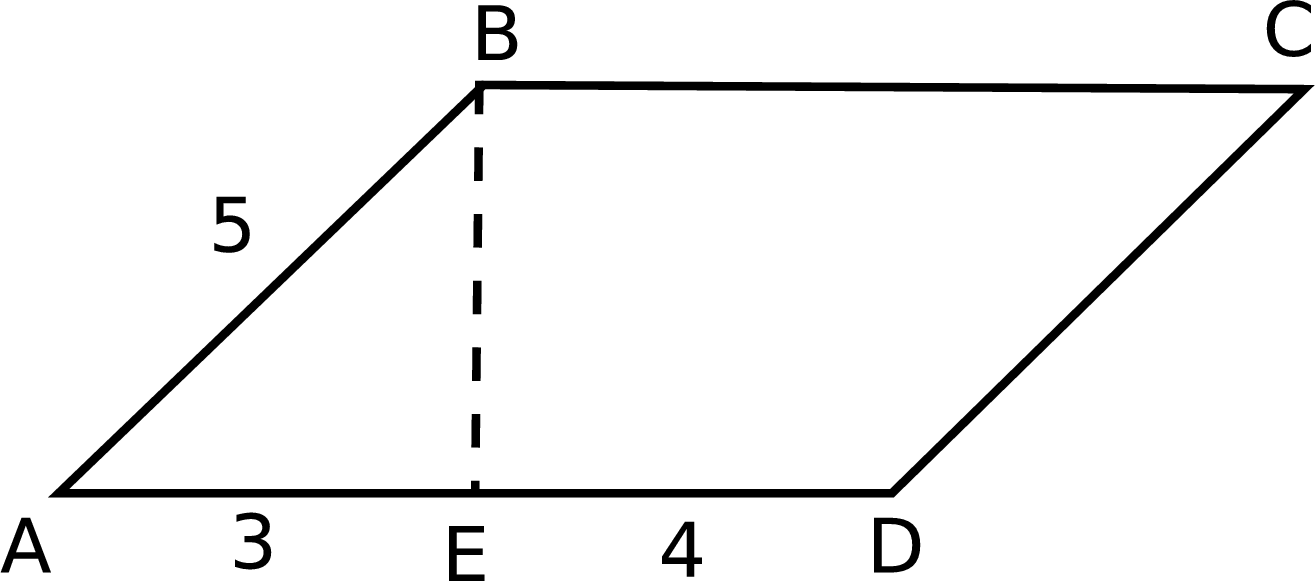
\includegraphics[width=300px]{col11306.imgs/m39357_area1.png} % m39357;area1.png;;;6.0;8.5;
        
      \vspace{2pt}
    \vspace{.1in}
    
    \end{center}

 \end{figure}   

    \addtocounter{footnote}{-0}
    
  \par 
\vspace{5pt}

\label{m39357*eip-208}\noindent\textbf{Solution to Exercise }
  \label{m39357*eip-995}\begin{enumerate}[noitemsep, label=\textbf{Step} \textbf{\arabic*}. ] 
            \leftskip=20pt\rightskip=\leftskip\item  We first need to find the height, BE, of the parallelogram. We can use Pythagoras to do this: 
\label{m39357*eip-id1165701596266}\nopagebreak\noindent{}\settowidth{\mymathboxwidth}{\begin{equation}
    \begin{array}{ccc}{\text{BE}}^{2}\hfill & =& {\text{AB}}^{2}-{\text{AE}}^{2}\hfill \\ \hfill {\text{BE}}^{2}& =& {5}^{2}-{3}^{2}\hfill \\ \hfill {\text{BE}}^{2}& =& 16\hfill \\ \hfill \text{BE}& =& 4\hfill \end{array}\tag{13.17}
      \end{equation}
    }
    \typeout{Columnwidth = \the\columnwidth}\typeout{math as usual width = \the\mymathboxwidth}
    \ifthenelse{\lengthtest{\mymathboxwidth < \columnwidth}}{% if the math fits, do it again, for real
    \begin{equation}
    \begin{array}{ccc}{\text{BE}}^{2}\hfill & =& {\text{AB}}^{2}-{\text{AE}}^{2}\hfill \\ \hfill {\text{BE}}^{2}& =& {5}^{2}-{3}^{2}\hfill \\ \hfill {\text{BE}}^{2}& =& 16\hfill \\ \hfill \text{BE}& =& 4\hfill \end{array}\tag{13.17}
      \end{equation}
    }{% else, if it doesn't fit
    \setlength{\mymathboxwidth}{\columnwidth}
      \addtolength{\mymathboxwidth}{-48pt}
    \par\vspace{12pt}\noindent\begin{minipage}{\columnwidth}
    \parbox[t]{\mymathboxwidth}{\large\begin{math}
    {\text{BE}}^{2}={\text{AB}}^{2}-{\text{AE}}^{2}{\text{BE}}^{2}={5}^{2}-{3}^{2}{\text{BE}}^{2}=16\text{BE}=4\end{math}}\hfill
    \parbox[t]{48pt}{\raggedleft 
    (13.17)}
    \end{minipage}\vspace{12pt}\par
    }% end of conditional for this bit of math
    \typeout{math as usual width = \the\mymathboxwidth}
    \item We apply the formula for the area of a parallelogram to find the area:
      \label{m39357*id1166232495800}\nopagebreak\noindent{}
        \settowidth{\mymathboxwidth}{\begin{equation}
    \begin{array}{ccc}\hfill \text{Area}& =& h\ensuremath{\times}b\hfill \\ & =& 4\ensuremath{\times}7\hfill \\ & =& 28\hfill \end{array}\tag{13.18}
      \end{equation}
    }
    \typeout{Columnwidth = \the\columnwidth}\typeout{math as usual width = \the\mymathboxwidth}
    \ifthenelse{\lengthtest{\mymathboxwidth < \columnwidth}}{% if the math fits, do it again, for real
    \begin{equation}
    \begin{array}{ccc}\hfill \text{Area}& =& h\ensuremath{\times}b\hfill \\ & =& 4\ensuremath{\times}7\hfill \\ & =& 28\hfill \end{array}\tag{13.18}
      \end{equation}
    }{% else, if it doesn't fit
    \setlength{\mymathboxwidth}{\columnwidth}
      \addtolength{\mymathboxwidth}{-48pt}
    \par\vspace{12pt}\noindent\begin{minipage}{\columnwidth}
    \parbox[t]{\mymathboxwidth}{\large\begin{math}
    \text{Area}=h\ensuremath{\times}b=4\ensuremath{\times}7=28\end{math}}\hfill
    \parbox[t]{48pt}{\raggedleft 
    (13.18)}
    \end{minipage}\vspace{12pt}\par
    }% end of conditional for this bit of math
    \typeout{math as usual width = \the\mymathboxwidth}
    
      \end{enumerate}
        


    \end{exercise}
    \end{mdframed}
    }
    \noindent
  \label{m39357*secfhsst!!!underscore!!!id1097}
            \subsubsection{  Polygons }
            \nopagebreak
            
          \label{m39357*id319959}\begin{enumerate}[noitemsep, label=\textbf{\arabic*}. ] 
            \label{m39357*uid104}\item For each case below, say whether the statement is true or false. For false statements, give a counter-example to prove it:
\label{m39357*id319975}\begin{enumerate}[noitemsep, label=\textbf{\alph*}. ] 
            \label{m39357*uid10566}\item All squares are rectangles
\label{m39357*uid10666}\item All rectangles are squares
\label{m39357*uid10766}\item All pentagons are similar
\label{m39357*uid10866}\item All equilateral triangles are similar
\label{m39357*uid10966}\item All pentagons are congruent
\label{m39357*uid11066}\item All equilateral triangles are congruent
\end{enumerate}
                \label{m39357*uid111666}\item Find the areas of each of the given figures - remember area is measured in square units (cm\begin{math}{}^{2}\end{math}, m\begin{math}{}^{2}\end{math}, mm\begin{math}{}^{2}\end{math}).

    \setcounter{subfigure}{0}


	\begin{figure}[H] % horizontal\label{m39357*id320109}
    \begin{center}
    \label{m39357*id320109!!!underscore!!!media}\label{m39357*id320109!!!underscore!!!printimage}\includegraphics{col11306.imgs/m39357_MG10C13_064.png} % m39357;MG10C13\_064.png;;;6.0;8.5;
        
      \vspace{2pt}
    \vspace{.1in}
    
    \end{center}

 \end{figure}   

    \addtocounter{footnote}{-0}
            \end{enumerate}
        
          

        
      

\label{m39357*id73452}
\par \raisebox{-5 pt}{
\includegraphics[width=0.5cm]{col11306.imgs/summary_www.png}} Find the answers with the shortcodes:
 \par \begin{tabular}[h]{cccccc}
 (1.) lxJ  &  (2.) lxS  & \end{tabular}



            \subsection{ Right prisms and cylinders}
            \nopagebreak
            
      \label{m39357*id62680}In this section we study how to calculate the surface areas and volumes of right prisms and cylinders. A right prism is a polygon that has been stretched out into a tube so that the height of the tube is perpendicular to the base (the definition is motivated by the fact that the angle between base and side form a right angle). A square prism has a base that is a square and a triangular prism has a base that is a triangle.\par 
      
    \setcounter{subfigure}{0}


	\begin{figure}[H] % horizontal\label{m39357*uid10}
    \begin{center}
    \rule[.1in]{\figurerulewidth}{.005in} \\
        \label{m39357*uid10!!!underscore!!!media}\label{m39357*uid10!!!underscore!!!printimage}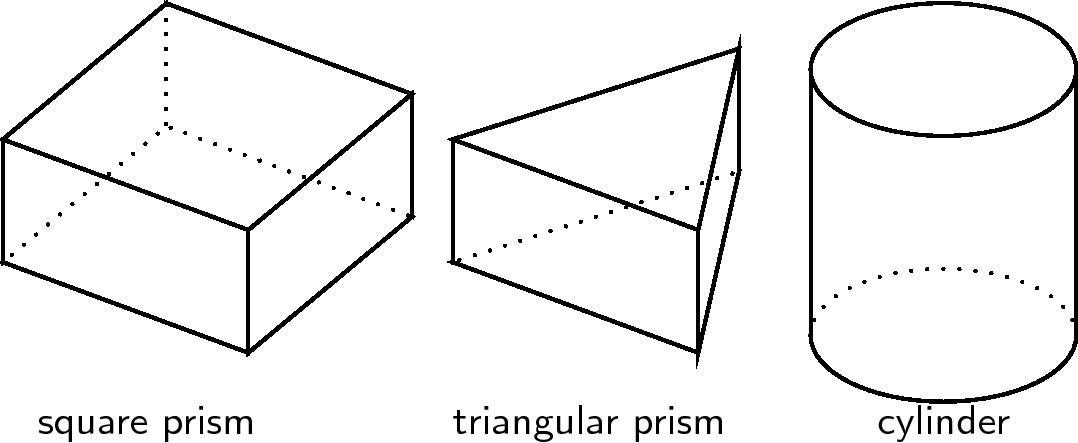
\includegraphics[width=300px]{col11306.imgs/m39357_MG10C14_001.png} % m39357;MG10C14\_001.png;;;6.0;8.5;
        
      \vspace{2pt}
    \vspace{\rubberspace}\par \begin{cnxcaption}
	  \small \textbf{Figure 13.24: }Examples of a right square prism, a right triangular prism and a cylinder.
	\end{cnxcaption}
      
    \vspace{.1in}
    \rule[.1in]{\figurerulewidth}{.005in} \\
        
    \end{center}

 \end{figure}   

    \addtocounter{footnote}{-0}
    
      \label{m39357*id62698}It is relatively simple to calculate the surface areas and volumes of prisms.\par 
      \label{m39357*uid11}
            \subsubsection{ Surface Area}
            \nopagebreak
            
        
        \label{m39357*id62710}The term \textsl{surface area} refers to the total area of the exposed or outside surfaces of a prism. This is easier to understand if you imagine the prism as a solid object.\par 
        \label{m39357*id62720}If you examine the prisms in Figure~13.24, you will see that each face of a prism is a simple polygon. For example, the triangular prism has two faces that are triangles and three faces that are rectangles. Therefore, in order to calculate the surface area of a prism you simply have to calculate the area of each face and add it up. In the case of a cylinder the top and bottom faces are circles, while the curved surface flattens into a rectangle.\par 
        \label{m39357*id62732}
          \textbf{Surface Area of Prisms}
        \par 
        \label{m39357*id62738}Calculate the area of each face and add the areas together to get the surface area. To do this you need to determine the correct shape of each and every face of the prism and then for each one determine the surface area. The sum of the surface areas of all the faces will give you the total surface area of the prism.\par 
\label{m39357*secfhsst!!!underscore!!!id107}
            \subsubsection{  Discussion : surface areas }
            \nopagebreak
            
        \label{m39357*id62753}In pairs, study the following prisms and the adjacent image showing the various surfaces that make up the prism. Explain to your partner, how each relates to the other.\par 
        
        \label{m39357*id6274366}
    \setcounter{subfigure}{0}


	\begin{figure}[H] % horizontal\label{m39357*id62767}
    \begin{center}
    \label{m39357*id62767!!!underscore!!!media}\label{m39357*id62767!!!underscore!!!printimage}\includegraphics{col11306.imgs/m39357_MG10C14_002.png} % m39357;MG10C14\_002.png;;;6.0;8.5;
        
      \vspace{2pt}
    \vspace{.1in}
    
    \end{center}

 \end{figure}   

    \addtocounter{footnote}{-0}
    
 \par 

\label{m39357*eip-630}
            \subsubsection{ Activity: Surface areas}
            \nopagebreak
            \label{m39357*eip-802}
Find (or take one yourself) a picture of a building that does not have a well defined shape (i.e. is not simply a rectangle). For example a castle with towers, or a house with gable windows or a porch. Assume you have to paint the outside of the building. How much paint would you need? Think about what you have learnt about surface area and the area of polygons. Can you find regular polygons on your picture and use those to find the surface area?
\par \label{m39357*secfhsst!!!underscore!!!id113}
            \subsubsection{  Surface areas }
            \nopagebreak
            
        \label{m39357*id62786}\begin{enumerate}[noitemsep, label=\textbf{\arabic*}. ] 
            \label{m39357*uid12}\item Calculate the surface area in each of the following:

    \setcounter{subfigure}{0}


	\begin{figure}[H] % horizontal\label{m39357*id62804}
    \begin{center}
    \label{m39357*id62804!!!underscore!!!media}\label{m39357*id62804!!!underscore!!!printimage}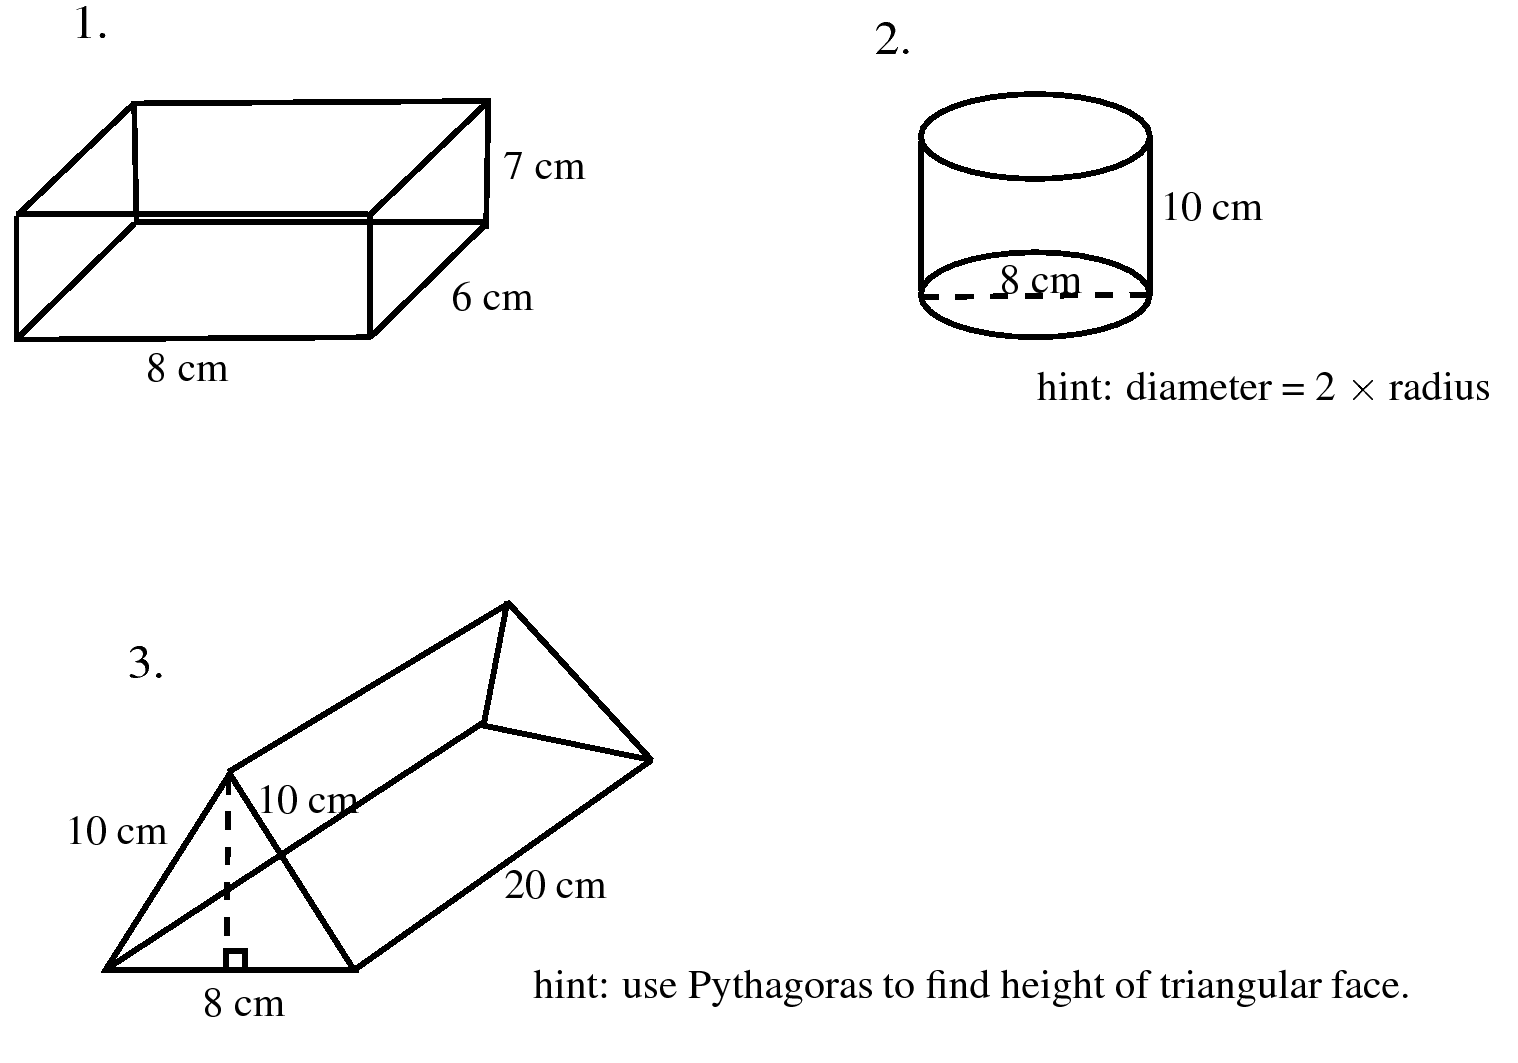
\includegraphics[width=300px]{col11306.imgs/m39357_MG10C14_003.png} % m39357;MG10C14\_003.png;;;6.0;8.5;
        
      \vspace{2pt}
    \vspace{.1in}
    
    \end{center}

 \end{figure}   

    \addtocounter{footnote}{-0}
            \label{m39357*uid13}\item  If a litre of paint covers an area of \begin{math}2{m}^{2}\end{math}, how much paint does a painter need to cover:
\label{m39357*id62841}\begin{enumerate}[noitemsep, label=\textbf{\alph*}. ] 
            \label{m39357*uid14}\item A rectangular swimming pool with dimensions \begin{math}4m\ensuremath{\times}3m\ensuremath{\times}2,5m\end{math}, inside walls and floor only.
\label{m39357*uid15}\item The inside walls and floor
of a circular reservoir with diameter \begin{math}4m\end{math} and height \begin{math}2,5m\end{math}\end{enumerate}
        
    \setcounter{subfigure}{0}


	\begin{figure}[H] % horizontal\label{m39357*id62926}
    \begin{center}
    \label{m39357*id62926!!!underscore!!!media}\label{m39357*id62926!!!underscore!!!printimage}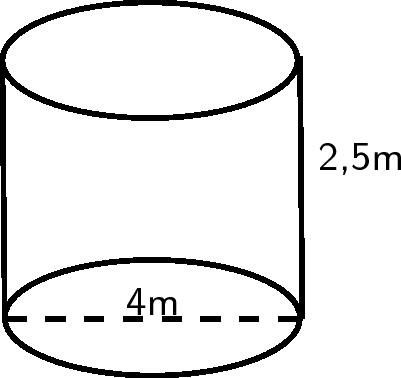
\includegraphics[width=300px]{col11306.imgs/m39357_MG10C14_004.png} % m39357;MG10C14\_004.png;;;6.0;8.5;
        
      \vspace{2pt}
    \vspace{.1in}
    
    \end{center}

 \end{figure}   

    \addtocounter{footnote}{-0}
            \end{enumerate}
        
        

      
      \label{m39357*uid16}
\par \raisebox{-5 pt}{
\includegraphics[width=0.5cm]{col11306.imgs/summary_www.png}} Find the answers with the shortcodes:
 \par \begin{tabular}[h]{cccccc}
 (1.) lT2  &  (2.) lq6  & \end{tabular}



            \subsubsection{ Volume}
            \nopagebreak
            \label{m39357*id62951}The volume of a right prism is calculated by multiplying the area of the base by the height. So, for a square prism of side length \begin{math}a\end{math} and height \begin{math}h\end{math} the volume is \begin{math}a\ensuremath{\times}a\ensuremath{\times}h={a}^{2}h\end{math}.\par 
        \label{m39357*id63000}
          \textbf{Volume of Prisms}
        \par 
        \label{m39357*id63006}Calculate the area of the base and multiply by the height to get the volume of a prism.\par 
\label{m39357*eip-491}\vspace{.5cm} 
      
      \noindent
      \hspace*{-30pt}
\includegraphics[width=0.5in]{col11306.imgs/pspencil2.png}   \raisebox{25mm}{   
      \begin{mdframed}[linewidth=4, leftmargin=40, rightmargin=40]  
      \begin{exercise}
    \noindent\textbf{Exercise 13.6}\label{m39357*eip-115}
  \label{m39357*eip-540}
  Find the surface area and volume for the a square prism of height \begin{math}4\phantom{\rule{2pt}{0ex}}\mathrm{cm}\end{math} and base length, \begin{math}3\phantom{\rule{2pt}{0ex}}\mathrm{cm}\end{math}.

    \setcounter{subfigure}{0}


	\begin{figure}[H] % horizontal\label{m39357*id6348}
    \begin{center}
    \label{m39357*id6348!!!underscore!!!media}\label{m39357*id6348!!!underscore!!!printimage}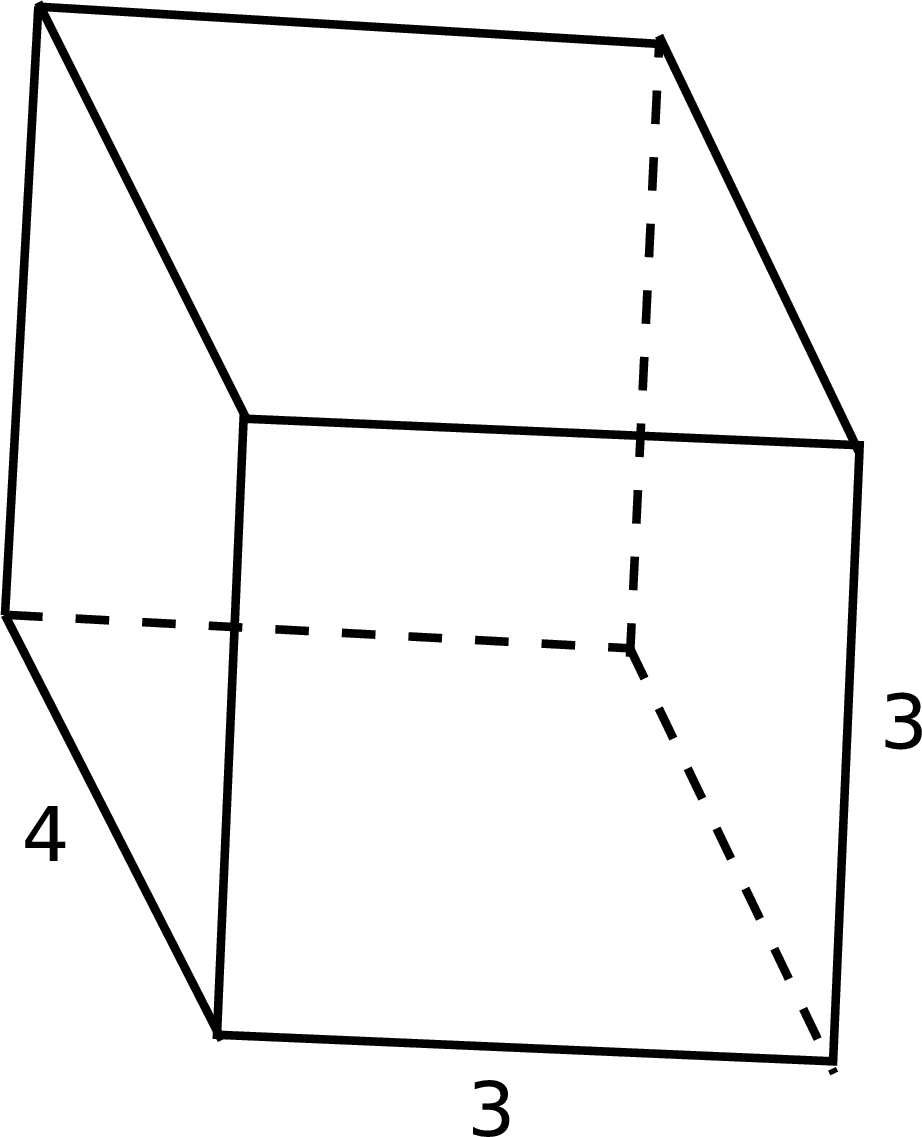
\includegraphics[height=300px]{col11306.imgs/m39357_squareprism.png} % m39357;squareprism.png;;;6.0;8.5;
        
      \vspace{2pt}
    \vspace{.1in}
    
    \end{center}

 \end{figure}   

    \addtocounter{footnote}{-0}
    
  \par 
\vspace{5pt}

\label{m39357*eip-51}\noindent\textbf{Solution to Exercise }
  \label{m39357*eip-226}\begin{enumerate}[noitemsep, label=\textbf{Step} \textbf{\arabic*}. ] 
            \leftskip=20pt\rightskip=\leftskip\item We use the formula for the surface area of a prism:
      \label{m39357*id1166229703568}\nopagebreak\noindent{}
        \settowidth{\mymathboxwidth}{\begin{equation}
    \begin{array}{ccc}\hfill \mathrm{S.A.}& =& 2\left[2\left(L\ensuremath{\times}b\right)+\left(b\ensuremath{\times}h\right)\right]\hfill \\ & =& 2\left[2\left(3\ensuremath{\times}4\right)+\left(3\ensuremath{\times}4\right)\right]\hfill \\ & =& {72\phantom{\rule{2pt}{0ex}}\mathrm{cm}}^{2}\hfill \end{array}\tag{13.19}
      \end{equation}
    }
    \typeout{Columnwidth = \the\columnwidth}\typeout{math as usual width = \the\mymathboxwidth}
    \ifthenelse{\lengthtest{\mymathboxwidth < \columnwidth}}{% if the math fits, do it again, for real
    \begin{equation}
    \begin{array}{ccc}\hfill \mathrm{S.A.}& =& 2\left[2\left(L\ensuremath{\times}b\right)+\left(b\ensuremath{\times}h\right)\right]\hfill \\ & =& 2\left[2\left(3\ensuremath{\times}4\right)+\left(3\ensuremath{\times}4\right)\right]\hfill \\ & =& {72\phantom{\rule{2pt}{0ex}}\mathrm{cm}}^{2}\hfill \end{array}\tag{13.19}
      \end{equation}
    }{% else, if it doesn't fit
    \setlength{\mymathboxwidth}{\columnwidth}
      \addtolength{\mymathboxwidth}{-48pt}
    \par\vspace{12pt}\noindent\begin{minipage}{\columnwidth}
    \parbox[t]{\mymathboxwidth}{\large\begin{math}
    \mathrm{S.A.}=2\left[2\left(L\ensuremath{\times}b\right)+\left(b\ensuremath{\times}h\right)\right]=2\left[2\left(3\ensuremath{\times}4\right)+\left(3\ensuremath{\times}4\right)\right]={72\phantom{\rule{2pt}{0ex}}\mathrm{cm}}^{2}\end{math}}\hfill
    \parbox[t]{48pt}{\raggedleft 
    (13.19)}
    \end{minipage}\vspace{12pt}\par
    }% end of conditional for this bit of math
    \typeout{math as usual width = \the\mymathboxwidth}
    
      \item To find the volume of the prism, we find the area of the base and multiply it by the height:
      \label{m39357*id1166232868439}\nopagebreak\noindent{}
        \settowidth{\mymathboxwidth}{\begin{equation}
    \begin{array}{ccc}V\hfill & =& {l}^{2}\ensuremath{\times}h\\ & =& \left({3}^{2}\right)\ensuremath{\times}4\hfill \\ & =& {36\phantom{\rule{2pt}{0ex}}\mathrm{cm}}^{3}\hfill \end{array}\tag{13.20}
      \end{equation}
    }
    \typeout{Columnwidth = \the\columnwidth}\typeout{math as usual width = \the\mymathboxwidth}
    \ifthenelse{\lengthtest{\mymathboxwidth < \columnwidth}}{% if the math fits, do it again, for real
    \begin{equation}
    \begin{array}{ccc}V\hfill & =& {l}^{2}\ensuremath{\times}h\\ & =& \left({3}^{2}\right)\ensuremath{\times}4\hfill \\ & =& {36\phantom{\rule{2pt}{0ex}}\mathrm{cm}}^{3}\hfill \end{array}\tag{13.20}
      \end{equation}
    }{% else, if it doesn't fit
    \setlength{\mymathboxwidth}{\columnwidth}
      \addtolength{\mymathboxwidth}{-48pt}
    \par\vspace{12pt}\noindent\begin{minipage}{\columnwidth}
    \parbox[t]{\mymathboxwidth}{\large\begin{math}
    V={l}^{2}\ensuremath{\times}h=\left({3}^{2}\right)\ensuremath{\times}4={36\phantom{\rule{2pt}{0ex}}\mathrm{cm}}^{3}\end{math}}\hfill
    \parbox[t]{48pt}{\raggedleft 
    (13.20)}
    \end{minipage}\vspace{12pt}\par
    }% end of conditional for this bit of math
    \typeout{math as usual width = \the\mymathboxwidth}
    
      \end{enumerate}
        


    \end{exercise}
    \end{mdframed}
    }
    \noindent
  \label{m39357*secfhsst!!!underscore!!!id132}
            \subsubsection{  Volume }
            \nopagebreak
            
        \label{m39357*id63019}\begin{enumerate}[noitemsep, label=\textbf{\arabic*}. ] 
            \label{m39357*uid17}\item Write down the formula for each of the following volumes:

    \setcounter{subfigure}{0}


	\begin{figure}[H] % horizontal\label{m39357*id63037}
    \begin{center}
    \label{m39357*id63037!!!underscore!!!media}\label{m39357*id63037!!!underscore!!!printimage}\includegraphics{col11306.imgs/m39357_MG10C14_005.png} % m39357;MG10C14\_005.png;;;6.0;8.5;
        
      \vspace{2pt}
    \vspace{.1in}
    
    \end{center}

 \end{figure}   

    \addtocounter{footnote}{-0}
            \label{m39357*uid18}\item Calculate the following volumes:

    \setcounter{subfigure}{0}


	\begin{figure}[H] % horizontal\label{m39357*id63058}
    \begin{center}
    \label{m39357*id63058!!!underscore!!!media}\label{m39357*id63058!!!underscore!!!printimage}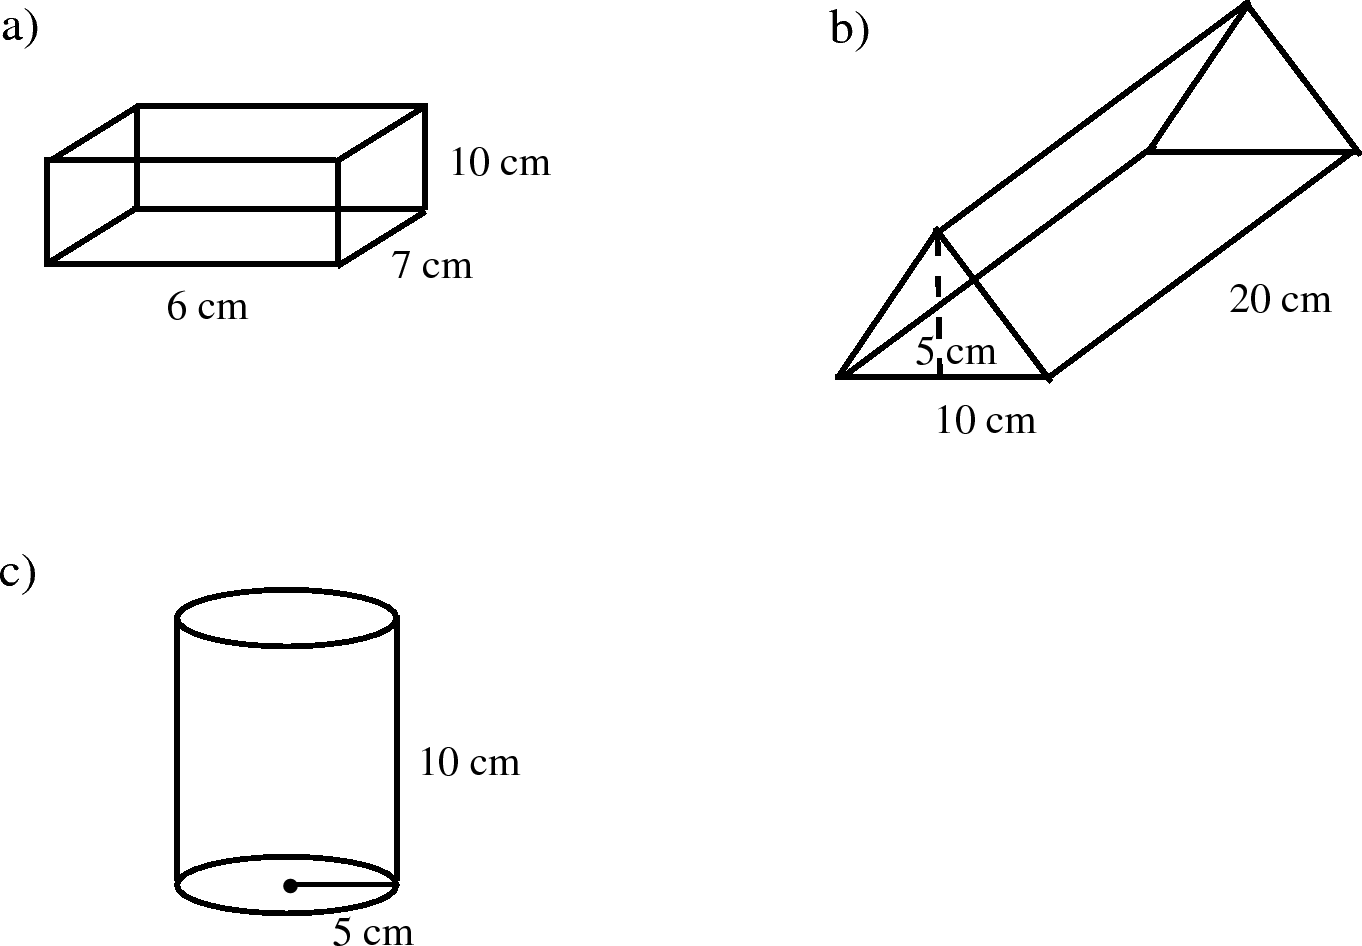
\includegraphics[width=300px]{col11306.imgs/m39357_MG10C14_006.png} % m39357;MG10C14\_006.png;;;6.0;8.5;
        
      \vspace{2pt}
    \vspace{.1in}
    
    \end{center}

 \end{figure}   

    \addtocounter{footnote}{-0}
            \label{m39357*uid19}\item A cube is a special prism that has all edges equal. This means that each face is a square. An example of a cube is a die. Show that for a cube with side length \begin{math}a\end{math}, the surface area is \begin{math}6{a}^{2}\end{math} and the volume is \begin{math}{a}^{3}\end{math}.

    \setcounter{subfigure}{0}


	\begin{figure}[H] % horizontal\label{m39357*id63117}
    \begin{center}
    \label{m39357*id63117!!!underscore!!!media}\label{m39357*id63117!!!underscore!!!printimage}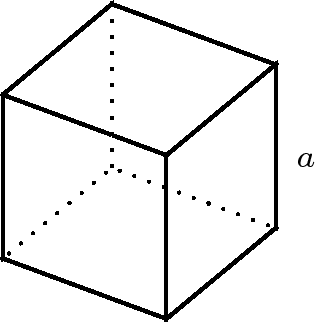
\includegraphics[height=300px]{col11306.imgs/m39357_MG10C14_007.png} % m39357;MG10C14\_007.png;;;6.0;8.5;
        
      \vspace{2pt}
    \vspace{.1in}
    
    \end{center}

 \end{figure}   

    \addtocounter{footnote}{-0}
            \end{enumerate}
        
        

        \label{m39357*id63133}Now, what happens to the surface area if one dimension is multiplied by a constant? For example, how does the surface area change when the height of a rectangular prism is divided by 2?\par 
 \label{m39357*is08324}       
    \setcounter{subfigure}{0}


	\begin{figure}[H] % horizontal\label{m39357*id63644234}
    \begin{center}
    \label{m39357*id63644234!!!underscore!!!media}\label{m39357*id63644234!!!underscore!!!printimage}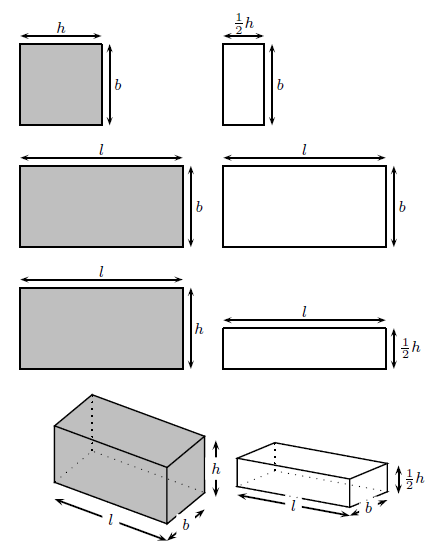
\includegraphics[height=300px]{col11306.imgs/m39357_MG10C14_008.png} % m39357;MG10C14\_008.png;;;6.0;8.5;
        
      \vspace{2pt}
    \vspace{\rubberspace}\par \begin{cnxcaption}
	  \small \textbf{Figure 13.32: }Rectangular prisms
	\end{cnxcaption}
      
    \vspace{.1in}
    
    \end{center}

 \end{figure}   

    \addtocounter{footnote}{-0}
    \par 
 
    % \textbf{m39357*eip-742}\par
    
    % how many colspecs?  2
          % name: cnx:colspec
            % colnum: 1
            % colwidth: 10*
            % latex-name: columna
            % colname: 
            % align/tgroup-align/default: //left
            % -------------------------
            % name: cnx:colspec
            % colnum: 2
            % colwidth: 10*
            % latex-name: columnb
            % colname: 
            % align/tgroup-align/default: //left
            % -------------------------
      
    
    \setlength\mytablespace{4\tabcolsep}
    \addtolength\mytablespace{3\arrayrulewidth}
    \setlength\mytablewidth{\linewidth}
        
    
    \setlength\mytableroom{\mytablewidth}
    \addtolength\mytableroom{-\mytablespace}
    
    \setlength\myfixedwidth{0pt}
    \setlength\mystarwidth{\mytableroom}
        \addtolength\mystarwidth{-\myfixedwidth}
        \divide\mystarwidth 20
        
    
      % ----- Begin capturing width of table in LR mode woof
      \settowidth{\mytableboxwidth}{\begin{tabular}[t]{|l|l|}\hline
    % count in rowspan-info-nodeset: 2
    % align/colidx: left,1
    
    % rowcount: '0' | start: 'false' | colidx: '1'
    
        % Formatting a regular cell and recurring on the next sibling
        \begin{math}\mathrm{Surface\; area}=2\left(l\ensuremath{\times}h+l\ensuremath{\times}b+b\ensuremath{\times}h\right)\end{math} &
      % align/colidx: left,2
    
    % rowcount: '0' | start: 'false' | colidx: '2'
    
        % Formatting a regular cell and recurring on the next sibling
        \begin{math}\mathrm{Surface\; area}=2\left(l\ensuremath{\times}\frac{1}{2}h+l\ensuremath{\times}b+b\ensuremath{\times}\frac{1}{2}h\right)\end{math}% make-rowspan-placeholders
    % rowspan info: col1 '0' | 'false' | '' || col2 '0' | 'false' | ''
     \tabularnewline\cline{1-1}\cline{2-2}
      %--------------------------------------------------------------------
    % align/colidx: left,1
    
    % rowcount: '0' | start: 'false' | colidx: '1'
    
        % Formatting a regular cell and recurring on the next sibling
        \begin{math}\mathrm{Volume}=l\ensuremath{\times}b\ensuremath{\times}h\end{math} &
      % align/colidx: left,2
    
    % rowcount: '0' | start: 'false' | colidx: '2'
    
        % Formatting a regular cell and recurring on the next sibling
        \begin{math}\begin{array}{ccc}\hfill \mathrm{Volume}& =& l\ensuremath{\times}b\ensuremath{\times}\frac{1}{2}h\hfill \\ & =& \frac{1}{2}\ensuremath{\times}l\ensuremath{\times}b\ensuremath{\times}h\hfill \end{array}\end{math}% make-rowspan-placeholders
    % rowspan info: col1 '0' | 'false' | '' || col2 '0' | 'false' | ''
     \tabularnewline\cline{1-1}\cline{2-2}
      %--------------------------------------------------------------------
    \end{tabular}} % end mytableboxwidth set
      \addtocounter{footnote}{-0}
      
      % ----- End capturing width of table in LR mode
    
        % ----- LR or paragraph mode: must test
        % ----- Begin capturing height of table
        \settoheight{\mytableboxheight}{\begin{tabular}[t]{|l|l|}\hline
    % count in rowspan-info-nodeset: 2
    % align/colidx: left,1
    
    % rowcount: '0' | start: 'false' | colidx: '1'
    
        % Formatting a regular cell and recurring on the next sibling
        \begin{math}\mathrm{Surface\; area}=2\left(l\ensuremath{\times}h+l\ensuremath{\times}b+b\ensuremath{\times}h\right)\end{math} &
      % align/colidx: left,2
    
    % rowcount: '0' | start: 'false' | colidx: '2'
    
        % Formatting a regular cell and recurring on the next sibling
        \begin{math}\mathrm{Surface\; area}=2\left(l\ensuremath{\times}\frac{1}{2}h+l\ensuremath{\times}b+b\ensuremath{\times}\frac{1}{2}h\right)\end{math}% make-rowspan-placeholders
    % rowspan info: col1 '0' | 'false' | '' || col2 '0' | 'false' | ''
     \tabularnewline\cline{1-1}\cline{2-2}
      %--------------------------------------------------------------------
    % align/colidx: left,1
    
    % rowcount: '0' | start: 'false' | colidx: '1'
    
        % Formatting a regular cell and recurring on the next sibling
        \begin{math}\mathrm{Volume}=l\ensuremath{\times}b\ensuremath{\times}h\end{math} &
      % align/colidx: left,2
    
    % rowcount: '0' | start: 'false' | colidx: '2'
    
        % Formatting a regular cell and recurring on the next sibling
        \begin{math}\begin{array}{ccc}\hfill \mathrm{Volume}& =& l\ensuremath{\times}b\ensuremath{\times}\frac{1}{2}h\hfill \\ & =& \frac{1}{2}\ensuremath{\times}l\ensuremath{\times}b\ensuremath{\times}h\hfill \end{array}\end{math}% make-rowspan-placeholders
    % rowspan info: col1 '0' | 'false' | '' || col2 '0' | 'false' | ''
     \tabularnewline\cline{1-1}\cline{2-2}
      %--------------------------------------------------------------------
    \end{tabular}} % end mytableboxheight set
        \settodepth{\mytableboxdepth}{\begin{tabular}[t]{|l|l|}\hline
    % count in rowspan-info-nodeset: 2
    % align/colidx: left,1
    
    % rowcount: '0' | start: 'false' | colidx: '1'
    
        % Formatting a regular cell and recurring on the next sibling
        \begin{math}\mathrm{Surface\; area}=2\left(l\ensuremath{\times}h+l\ensuremath{\times}b+b\ensuremath{\times}h\right)\end{math} &
      % align/colidx: left,2
    
    % rowcount: '0' | start: 'false' | colidx: '2'
    
        % Formatting a regular cell and recurring on the next sibling
        \begin{math}\mathrm{Surface\; area}=2\left(l\ensuremath{\times}\frac{1}{2}h+l\ensuremath{\times}b+b\ensuremath{\times}\frac{1}{2}h\right)\end{math}% make-rowspan-placeholders
    % rowspan info: col1 '0' | 'false' | '' || col2 '0' | 'false' | ''
     \tabularnewline\cline{1-1}\cline{2-2}
      %--------------------------------------------------------------------
    % align/colidx: left,1
    
    % rowcount: '0' | start: 'false' | colidx: '1'
    
        % Formatting a regular cell and recurring on the next sibling
        \begin{math}\mathrm{Volume}=l\ensuremath{\times}b\ensuremath{\times}h\end{math} &
      % align/colidx: left,2
    
    % rowcount: '0' | start: 'false' | colidx: '2'
    
        % Formatting a regular cell and recurring on the next sibling
        \begin{math}\begin{array}{ccc}\hfill \mathrm{Volume}& =& l\ensuremath{\times}b\ensuremath{\times}\frac{1}{2}h\hfill \\ & =& \frac{1}{2}\ensuremath{\times}l\ensuremath{\times}b\ensuremath{\times}h\hfill \end{array}\end{math}% make-rowspan-placeholders
    % rowspan info: col1 '0' | 'false' | '' || col2 '0' | 'false' | ''
     \tabularnewline\cline{1-1}\cline{2-2}
      %--------------------------------------------------------------------
    \end{tabular}} % end mytableboxdepth set
        \addtolength{\mytableboxheight}{\mytableboxdepth}
        % ----- End capturing height of table
        \addtocounter{footnote}{-0}
        
        \ifthenelse{\mytableboxwidth<\textwidth}{% the table fits in LR mode
          \addtolength{\mytableboxwidth}{-\mytablespace}
          \typeout{textheight: \the\textheight}
          \typeout{mytableboxheight: \the\mytableboxheight}
          \typeout{textwidth: \the\textwidth}
          \typeout{mytableboxwidth: \the\mytableboxwidth}
          \ifthenelse{\mytableboxheight<\textheight}{%
        
    % \begin{table}[H]
    % \\ '' '0'
    
        \begin{center}
      
      \label{m39357*eip-742}
      
    \noindent
    \begin{tabular}[t]{|l|l|}\hline
    % count in rowspan-info-nodeset: 2
    % align/colidx: left,1
    
    % rowcount: '0' | start: 'false' | colidx: '1'
    
        % Formatting a regular cell and recurring on the next sibling
        \begin{math}\mathrm{Surface\; area}=2\left(l\ensuremath{\times}h+l\ensuremath{\times}b+b\ensuremath{\times}h\right)\end{math} &
      % align/colidx: left,2
    
    % rowcount: '0' | start: 'false' | colidx: '2'
    
        % Formatting a regular cell and recurring on the next sibling
        \begin{math}\mathrm{Surface\; area}=2\left(l\ensuremath{\times}\frac{1}{2}h+l\ensuremath{\times}b+b\ensuremath{\times}\frac{1}{2}h\right)\end{math}% make-rowspan-placeholders
    % rowspan info: col1 '0' | 'false' | '' || col2 '0' | 'false' | ''
     \tabularnewline\cline{1-1}\cline{2-2}
      %--------------------------------------------------------------------
    % align/colidx: left,1
    
    % rowcount: '0' | start: 'false' | colidx: '1'
    
        % Formatting a regular cell and recurring on the next sibling
        \begin{math}\mathrm{Volume}=l\ensuremath{\times}b\ensuremath{\times}h\end{math} &
      % align/colidx: left,2
    
    % rowcount: '0' | start: 'false' | colidx: '2'
    
        % Formatting a regular cell and recurring on the next sibling
        \begin{math}\begin{array}{ccc}\hfill \mathrm{Volume}& =& l\ensuremath{\times}b\ensuremath{\times}\frac{1}{2}h\hfill \\ & =& \frac{1}{2}\ensuremath{\times}l\ensuremath{\times}b\ensuremath{\times}h\hfill \end{array}\end{math}% make-rowspan-placeholders
    % rowspan info: col1 '0' | 'false' | '' || col2 '0' | 'false' | ''
     \tabularnewline\cline{1-1}\cline{2-2}
      %--------------------------------------------------------------------
    \end{tabular}
      \end{center}
    \begin{center}{\small\bfseries Table 13.2}\end{center}
    %\end{table}
    
    \addtocounter{footnote}{-0}
    
          }{ % else
        
    % \begin{table}[H]
    % \\ '' '0'
    
        \begin{center}
      
      \label{m39357*eip-742}
      
    \noindent
    \tabletail{%
        \hline
        \multicolumn{2}{|p{\mytableboxwidth}|}{\raggedleft \small \sl continued on next page}\\
        \hline
      }
      \tablelasttail{}
      \begin{xtabular}[t]{|l|l|}\hline
    % count in rowspan-info-nodeset: 2
    % align/colidx: left,1
    
    % rowcount: '0' | start: 'false' | colidx: '1'
    
        % Formatting a regular cell and recurring on the next sibling
        \begin{math}\mathrm{Surface\; area}=2\left(l\ensuremath{\times}h+l\ensuremath{\times}b+b\ensuremath{\times}h\right)\end{math} &
      % align/colidx: left,2
    
    % rowcount: '0' | start: 'false' | colidx: '2'
    
        % Formatting a regular cell and recurring on the next sibling
        \begin{math}\mathrm{Surface\; area}=2\left(l\ensuremath{\times}\frac{1}{2}h+l\ensuremath{\times}b+b\ensuremath{\times}\frac{1}{2}h\right)\end{math}% make-rowspan-placeholders
    % rowspan info: col1 '0' | 'false' | '' || col2 '0' | 'false' | ''
     \tabularnewline\cline{1-1}\cline{2-2}
      %--------------------------------------------------------------------
    % align/colidx: left,1
    
    % rowcount: '0' | start: 'false' | colidx: '1'
    
        % Formatting a regular cell and recurring on the next sibling
        \begin{math}\mathrm{Volume}=l\ensuremath{\times}b\ensuremath{\times}h\end{math} &
      % align/colidx: left,2
    
    % rowcount: '0' | start: 'false' | colidx: '2'
    
        % Formatting a regular cell and recurring on the next sibling
        \begin{math}\begin{array}{ccc}\hfill \mathrm{Volume}& =& l\ensuremath{\times}b\ensuremath{\times}\frac{1}{2}h\hfill \\ & =& \frac{1}{2}\ensuremath{\times}l\ensuremath{\times}b\ensuremath{\times}h\hfill \end{array}\end{math}% make-rowspan-placeholders
    % rowspan info: col1 '0' | 'false' | '' || col2 '0' | 'false' | ''
     \tabularnewline\cline{1-1}\cline{2-2}
      %--------------------------------------------------------------------
    \end{xtabular}
      \end{center}
    \begin{center}{\small\bfseries Table 13.2}\end{center}
    %\end{table}
    
    \addtocounter{footnote}{-0}
    
          } % 
        }{% else
        % typeset the table in paragraph mode
        % ----- Begin capturing height of table
        \settoheight{\mytableboxheight}{\begin{tabular*}{\mytablewidth}[t]{|p{10\mystarwidth}|p{10\mystarwidth}|}\hline
    % count in rowspan-info-nodeset: 2
    % align/colidx: left,1
    
    % rowcount: '0' | start: 'false' | colidx: '1'
    
        % Formatting a regular cell and recurring on the next sibling
        \begin{math}\mathrm{Surface\; area}=2\left(l\ensuremath{\times}h+l\ensuremath{\times}b+b\ensuremath{\times}h\right)\end{math} &
      % align/colidx: left,2
    
    % rowcount: '0' | start: 'false' | colidx: '2'
    
        % Formatting a regular cell and recurring on the next sibling
        \begin{math}\mathrm{Surface\; area}=2\left(l\ensuremath{\times}\frac{1}{2}h+l\ensuremath{\times}b+b\ensuremath{\times}\frac{1}{2}h\right)\end{math}% make-rowspan-placeholders
    % rowspan info: col1 '0' | 'false' | '' || col2 '0' | 'false' | ''
     \tabularnewline\cline{1-1}\cline{2-2}
      %--------------------------------------------------------------------
    % align/colidx: left,1
    
    % rowcount: '0' | start: 'false' | colidx: '1'
    
        % Formatting a regular cell and recurring on the next sibling
        \begin{math}\mathrm{Volume}=l\ensuremath{\times}b\ensuremath{\times}h\end{math} &
      % align/colidx: left,2
    
    % rowcount: '0' | start: 'false' | colidx: '2'
    
        % Formatting a regular cell and recurring on the next sibling
        \begin{math}\begin{array}{ccc}\hfill \mathrm{Volume}& =& l\ensuremath{\times}b\ensuremath{\times}\frac{1}{2}h\hfill \\ & =& \frac{1}{2}\ensuremath{\times}l\ensuremath{\times}b\ensuremath{\times}h\hfill \end{array}\end{math}% make-rowspan-placeholders
    % rowspan info: col1 '0' | 'false' | '' || col2 '0' | 'false' | ''
     \tabularnewline\cline{1-1}\cline{2-2}
      %--------------------------------------------------------------------
    \end{tabular*}} % end mytableboxheight set
        \settodepth{\mytableboxdepth}{\begin{tabular*}{\mytablewidth}[t]{|p{10\mystarwidth}|p{10\mystarwidth}|}\hline
    % count in rowspan-info-nodeset: 2
    % align/colidx: left,1
    
    % rowcount: '0' | start: 'false' | colidx: '1'
    
        % Formatting a regular cell and recurring on the next sibling
        \begin{math}\mathrm{Surface\; area}=2\left(l\ensuremath{\times}h+l\ensuremath{\times}b+b\ensuremath{\times}h\right)\end{math} &
      % align/colidx: left,2
    
    % rowcount: '0' | start: 'false' | colidx: '2'
    
        % Formatting a regular cell and recurring on the next sibling
        \begin{math}\mathrm{Surface\; area}=2\left(l\ensuremath{\times}\frac{1}{2}h+l\ensuremath{\times}b+b\ensuremath{\times}\frac{1}{2}h\right)\end{math}% make-rowspan-placeholders
    % rowspan info: col1 '0' | 'false' | '' || col2 '0' | 'false' | ''
     \tabularnewline\cline{1-1}\cline{2-2}
      %--------------------------------------------------------------------
    % align/colidx: left,1
    
    % rowcount: '0' | start: 'false' | colidx: '1'
    
        % Formatting a regular cell and recurring on the next sibling
        \begin{math}\mathrm{Volume}=l\ensuremath{\times}b\ensuremath{\times}h\end{math} &
      % align/colidx: left,2
    
    % rowcount: '0' | start: 'false' | colidx: '2'
    
        % Formatting a regular cell and recurring on the next sibling
        \begin{math}\begin{array}{ccc}\hfill \mathrm{Volume}& =& l\ensuremath{\times}b\ensuremath{\times}\frac{1}{2}h\hfill \\ & =& \frac{1}{2}\ensuremath{\times}l\ensuremath{\times}b\ensuremath{\times}h\hfill \end{array}\end{math}% make-rowspan-placeholders
    % rowspan info: col1 '0' | 'false' | '' || col2 '0' | 'false' | ''
     \tabularnewline\cline{1-1}\cline{2-2}
      %--------------------------------------------------------------------
    \end{tabular*}} % end mytableboxdepth set
        \addtolength{\mytableboxheight}{\mytableboxdepth}
        % ----- End capturing height of table
        \typeout{textheight: \the\textheight}
        \typeout{mytableboxheight: \the\mytableboxheight}
        \typeout{table too wide, outputting in para mode}
        
    % \begin{table}[H]
    % \\ '' '0'
    
        \begin{center}
      
      \label{m39357*eip-742}
      
    \noindent
    \tabletail{%
        \hline
        \multicolumn{2}{|p{\mytableroom}|}{\raggedleft \small \sl continued on next page}\\
        \hline
      }
      \tablelasttail{}
      \begin{xtabular*}{\mytablewidth}[t]{|p{10\mystarwidth}|p{10\mystarwidth}|}\hline
    % count in rowspan-info-nodeset: 2
    % align/colidx: left,1
    
    % rowcount: '0' | start: 'false' | colidx: '1'
    
        % Formatting a regular cell and recurring on the next sibling
        \begin{math}\mathrm{Surface\; area}=2\left(l\ensuremath{\times}h+l\ensuremath{\times}b+b\ensuremath{\times}h\right)\end{math} &
      % align/colidx: left,2
    
    % rowcount: '0' | start: 'false' | colidx: '2'
    
        % Formatting a regular cell and recurring on the next sibling
        \begin{math}\mathrm{Surface\; area}=2\left(l\ensuremath{\times}\frac{1}{2}h+l\ensuremath{\times}b+b\ensuremath{\times}\frac{1}{2}h\right)\end{math}% make-rowspan-placeholders
    % rowspan info: col1 '0' | 'false' | '' || col2 '0' | 'false' | ''
     \tabularnewline\cline{1-1}\cline{2-2}
      %--------------------------------------------------------------------
    % align/colidx: left,1
    
    % rowcount: '0' | start: 'false' | colidx: '1'
    
        % Formatting a regular cell and recurring on the next sibling
        \begin{math}\mathrm{Volume}=l\ensuremath{\times}b\ensuremath{\times}h\end{math} &
      % align/colidx: left,2
    
    % rowcount: '0' | start: 'false' | colidx: '2'
    
        % Formatting a regular cell and recurring on the next sibling
        \begin{math}\begin{array}{ccc}\hfill \mathrm{Volume}& =& l\ensuremath{\times}b\ensuremath{\times}\frac{1}{2}h\hfill \\ & =& \frac{1}{2}\ensuremath{\times}l\ensuremath{\times}b\ensuremath{\times}h\hfill \end{array}\end{math}% make-rowspan-placeholders
    % rowspan info: col1 '0' | 'false' | '' || col2 '0' | 'false' | ''
     \tabularnewline\cline{1-1}\cline{2-2}
      %--------------------------------------------------------------------
    \end{xtabular*}
      \end{center}
    \begin{center}{\small\bfseries Table 13.2}\end{center}
    %\end{table}
    
    \addtocounter{footnote}{-0}
    
        }% ending lr/para test clause
      
    \par
  
\par
            \label{m39357*secfhsst!!!underscore!!!id147}\vspace{.5cm} 
      
      \noindent
      \hspace*{-30pt}
\includegraphics[width=0.5in]{col11306.imgs/pspencil2.png}   \raisebox{25mm}{   
      \begin{mdframed}[linewidth=4, leftmargin=40, rightmargin=40]  
      \begin{exercise}
    \noindent\textbf{Exercise 13.7:  Scaling the dimensions of a prism }
        \label{m39357*probfhsst!!!underscore!!!id148}
        \label{m39357*id63614}The size of a prism is specified by the length of its sides. The prism in the diagram has sides of lengths \begin{math}L\end{math}, \begin{math}b\end{math} and \begin{math}h\end{math}.\par 
        \label{m39357*id63643}
          
    \setcounter{subfigure}{0}


	\begin{figure}[H] % horizontal\label{m39357*id63644}
    \begin{center}
    \label{m39357*id63644!!!underscore!!!media}\label{m39357*id63644!!!underscore!!!printimage}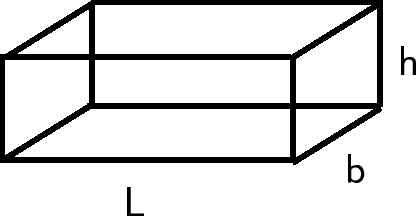
\includegraphics[width=300px]{col11306.imgs/m39357_MG10C14_009.png} % m39357;MG10C14\_009.png;;;6.0;8.5;
        
      \vspace{2pt}
    \vspace{.1in}
    
    \end{center}

 \end{figure}   

    \addtocounter{footnote}{-0}
    
        \par 
        \label{m39357*id63651}\begin{enumerate}[noitemsep, label=\textbf{\arabic*}. ] 
            \leftskip=20pt\rightskip=\leftskip\label{m39357*uid21}\item Consider enlarging all sides of the prism by a constant factor \begin{math}x\end{math}, where \begin{math}x\greatthan{}1\end{math}. Calculate the volume and surface area of the enlarged prism as a function of the factor \begin{math}x\end{math} and the volume of the original volume.
\label{m39357*uid22}\item In the same way as above now consider the case, where \begin{math}0\lessthan{}x\lessthan{}1\end{math}. Now calculate the reduction factor in the volume and the surface area.
\end{enumerate}
        
        
        \vspace{5pt}
        \label{m39357*solfhsst!!!underscore!!!id166}\noindent\textbf{Solution to Exercise } \label{m39357*listfhsst!!!underscore!!!id166}\begin{enumerate}[noitemsep, label=\textbf{Step} \textbf{\arabic*}. ] 
            \leftskip=20pt\rightskip=\leftskip\item  
        \label{m39357*id63750}The volume of a prism is given by:
\begin{math}V=L\ensuremath{\times}b\ensuremath{\times}h\end{math}\par 
        \label{m39357*id63774}The surface area of the prism is given by:
\begin{math}A=2\ensuremath{\times}\left(L\ensuremath{\times}b+L\ensuremath{\times}h+b\ensuremath{\times}h\right)\end{math}\par 
        \item  
        \label{m39357*id63826}If all the sides of the prism get rescaled, the new sides will be:\par 
        \label{m39357*id63830}\nopagebreak\noindent{}
          \settowidth{\mymathboxwidth}{\begin{equation}
    \begin{array}{ccc}\hfill {L}^{\text{'}}& =& x\ensuremath{\times}L\hfill \\ \hfill {b}^{\text{'}}& =& x\ensuremath{\times}b\hfill \\ \hfill {h}^{\text{'}}& =& x\ensuremath{\times}h\hfill \end{array}\tag{13.21}
      \end{equation}
    }
    \typeout{Columnwidth = \the\columnwidth}\typeout{math as usual width = \the\mymathboxwidth}
    \ifthenelse{\lengthtest{\mymathboxwidth < \columnwidth}}{% if the math fits, do it again, for real
    \begin{equation}
    \begin{array}{ccc}\hfill {L}^{\text{'}}& =& x\ensuremath{\times}L\hfill \\ \hfill {b}^{\text{'}}& =& x\ensuremath{\times}b\hfill \\ \hfill {h}^{\text{'}}& =& x\ensuremath{\times}h\hfill \end{array}\tag{13.21}
      \end{equation}
    }{% else, if it doesn't fit
    \setlength{\mymathboxwidth}{\columnwidth}
      \addtolength{\mymathboxwidth}{-48pt}
    \par\vspace{12pt}\noindent\begin{minipage}{\columnwidth}
    \parbox[t]{\mymathboxwidth}{\large\begin{math}
    {L}^{\text{'}}=x\ensuremath{\times}L{b}^{\text{'}}=x\ensuremath{\times}b{h}^{\text{'}}=x\ensuremath{\times}h\end{math}}\hfill
    \parbox[t]{48pt}{\raggedleft 
    (13.21)}
    \end{minipage}\vspace{12pt}\par
    }% end of conditional for this bit of math
    \typeout{math as usual width = \the\mymathboxwidth}
    
        
        \label{m39357*id63916}The new volume will then be given by:\par 
        \label{m39357*id63920}\nopagebreak\noindent{}
          \settowidth{\mymathboxwidth}{\begin{equation}
    \begin{array}{ccc}\hfill {V}^{\text{'}}& =& {L}^{\text{'}}\ensuremath{\times}{b}^{\text{'}}\ensuremath{\times}{h}^{\text{'}}\hfill \\ & =& x\ensuremath{\times}L\ensuremath{\times}x\ensuremath{\times}b\ensuremath{\times}x\ensuremath{\times}h\hfill \\ & =& {x}^{3}\ensuremath{\times}L\ensuremath{\times}b\ensuremath{\times}h\hfill \\ & =& {x}^{3}\ensuremath{\times}V\hfill \end{array}\tag{13.22}
      \end{equation}
    }
    \typeout{Columnwidth = \the\columnwidth}\typeout{math as usual width = \the\mymathboxwidth}
    \ifthenelse{\lengthtest{\mymathboxwidth < \columnwidth}}{% if the math fits, do it again, for real
    \begin{equation}
    \begin{array}{ccc}\hfill {V}^{\text{'}}& =& {L}^{\text{'}}\ensuremath{\times}{b}^{\text{'}}\ensuremath{\times}{h}^{\text{'}}\hfill \\ & =& x\ensuremath{\times}L\ensuremath{\times}x\ensuremath{\times}b\ensuremath{\times}x\ensuremath{\times}h\hfill \\ & =& {x}^{3}\ensuremath{\times}L\ensuremath{\times}b\ensuremath{\times}h\hfill \\ & =& {x}^{3}\ensuremath{\times}V\hfill \end{array}\tag{13.22}
      \end{equation}
    }{% else, if it doesn't fit
    \setlength{\mymathboxwidth}{\columnwidth}
      \addtolength{\mymathboxwidth}{-48pt}
    \par\vspace{12pt}\noindent\begin{minipage}{\columnwidth}
    \parbox[t]{\mymathboxwidth}{\large\begin{math}
    {V}^{\text{'}}={L}^{\text{'}}\ensuremath{\times}{b}^{\text{'}}\ensuremath{\times}{h}^{\text{'}}=x\ensuremath{\times}L\ensuremath{\times}x\ensuremath{\times}b\ensuremath{\times}x\ensuremath{\times}h={x}^{3}\ensuremath{\times}L\ensuremath{\times}b\ensuremath{\times}h={x}^{3}\ensuremath{\times}V\end{math}}\hfill
    \parbox[t]{48pt}{\raggedleft 
    (13.22)}
    \end{minipage}\vspace{12pt}\par
    }% end of conditional for this bit of math
    \typeout{math as usual width = \the\mymathboxwidth}
    
        
        \label{m39357*id64062}The new surface area of the prism will be given by:\par 
        \label{m39357*id64066}\nopagebreak\noindent{}
          \settowidth{\mymathboxwidth}{\begin{equation}
    \begin{array}{ccc}\hfill {A}^{\text{'}}& =& 2\ensuremath{\times}\left({L}^{\text{'}}\ensuremath{\times}{b}^{\text{'}}+{L}^{\text{'}}\ensuremath{\times}{h}^{\text{'}}+{b}^{\text{'}}\ensuremath{\times}{h}^{\text{'}}\right)\hfill \\ & =& 2\ensuremath{\times}\left(x\ensuremath{\times}L\ensuremath{\times}x\ensuremath{\times}b+x\ensuremath{\times}L\ensuremath{\times}x\ensuremath{\times}h+x\ensuremath{\times}b\ensuremath{\times}x\ensuremath{\times}h\right)\hfill \\ & =& {x}^{2}\ensuremath{\times}2\ensuremath{\times}\left(L\ensuremath{\times}b+L\ensuremath{\times}h+b\ensuremath{\times}h\right)\hfill \\ & =& {x}^{2}\ensuremath{\times}A\hfill \end{array}\tag{13.23}
      \end{equation}
    }
    \typeout{Columnwidth = \the\columnwidth}\typeout{math as usual width = \the\mymathboxwidth}
    \ifthenelse{\lengthtest{\mymathboxwidth < \columnwidth}}{% if the math fits, do it again, for real
    \begin{equation}
    \begin{array}{ccc}\hfill {A}^{\text{'}}& =& 2\ensuremath{\times}\left({L}^{\text{'}}\ensuremath{\times}{b}^{\text{'}}+{L}^{\text{'}}\ensuremath{\times}{h}^{\text{'}}+{b}^{\text{'}}\ensuremath{\times}{h}^{\text{'}}\right)\hfill \\ & =& 2\ensuremath{\times}\left(x\ensuremath{\times}L\ensuremath{\times}x\ensuremath{\times}b+x\ensuremath{\times}L\ensuremath{\times}x\ensuremath{\times}h+x\ensuremath{\times}b\ensuremath{\times}x\ensuremath{\times}h\right)\hfill \\ & =& {x}^{2}\ensuremath{\times}2\ensuremath{\times}\left(L\ensuremath{\times}b+L\ensuremath{\times}h+b\ensuremath{\times}h\right)\hfill \\ & =& {x}^{2}\ensuremath{\times}A\hfill \end{array}\tag{13.23}
      \end{equation}
    }{% else, if it doesn't fit
    \setlength{\mymathboxwidth}{\columnwidth}
      \addtolength{\mymathboxwidth}{-48pt}
    \par\vspace{12pt}\noindent\begin{minipage}{\columnwidth}
    \parbox[t]{\mymathboxwidth}{\large\begin{math}
    {A}^{\text{'}}=2\ensuremath{\times}\left({L}^{\text{'}}\ensuremath{\times}{b}^{\text{'}}+{L}^{\text{'}}\ensuremath{\times}{h}^{\text{'}}+{b}^{\text{'}}\ensuremath{\times}{h}^{\text{'}}\right)=2\ensuremath{\times}\left(x\ensuremath{\times}L\ensuremath{\times}x\ensuremath{\times}b+x\ensuremath{\times}L\ensuremath{\times}x\ensuremath{\times}h+x\ensuremath{\times}b\ensuremath{\times}x\ensuremath{\times}h\right)={x}^{2}\ensuremath{\times}2\ensuremath{\times}\left(L\ensuremath{\times}b+L\ensuremath{\times}h+b\ensuremath{\times}h\right)={x}^{2}\ensuremath{\times}A\end{math}}\hfill
    \parbox[t]{48pt}{\raggedleft 
    (13.23)}
    \end{minipage}\vspace{12pt}\par
    }% end of conditional for this bit of math
    \typeout{math as usual width = \the\mymathboxwidth}
    
        
        \item  
        \label{m39357*id64313}\begin{enumerate}[noitemsep, label=\textbf{\alph*}. ] 
            \leftskip=20pt\rightskip=\leftskip\label{m39357*uid23}\item We found above that the new volume is given by:
\begin{math}{V}^{\text{'}}={x}^{3}\ensuremath{\times}V\end{math}
Since \begin{math}x\greatthan{}1\end{math}, the volume of the prism will be increased by a factor of \begin{math}{x}^{3}\end{math}.
The surface area of the rescaled prism was given by:
\begin{math}{A}^{\text{'}}={x}^{2}\ensuremath{\times}A\end{math}
Again, since \begin{math}x\greatthan{}1\end{math}, the surface area will be increased by a factor of \begin{math}{x}^{2}\end{math}. Surface areas which are two dimensional increase with the square of the factor while volumes, which are three dimensional, increase with the cube of the factor.
\label{m39357*uid24}\item The answer here is based on the same ideas as above.
In analogy, since here \begin{math}0\lessthan{}x\lessthan{}1\end{math}, the volume will be reduced by a factor of \begin{math}{x}^{3}\end{math} and the surface area will be decreased by a factor of \begin{math}{x}^{2}\end{math}\end{enumerate}
        
        
        \end{enumerate}
         

    \end{exercise}
    \end{mdframed}
    }
    \noindent
  
        \label{m39357*id64533}When the length of one of the sides is multiplied by a constant the effect is to multiply the original volume by that constant, as for the example in Figure~13.32.\par 
      
    

  \label{m39357*cid323}
\par \raisebox{-5 pt}{\includegraphics[width=0.5cm]{col11306.imgs/summary_www.png}} Find the answers with the shortcodes:
 \par \begin{tabular}[h]{cccccc}
 (1.) lTk  &  (2.) lT0  &  (3.) lTT  & \end{tabular}



            \subsection{ Right Pyramids, Right Cones and Spheres}
            \nopagebreak
            
      
      \label{m39357*id62623}A pyramid is a geometric solid that has a polygon base and the base is joined to a point, called the apex. Two examples of pyramids are shown in the left-most and centre figures in . The right-most figure has an apex which is joined to a circular base and this type of geometric solid is called a cone. Cones are similar to pyramids except that their bases are circles instead of polygons.\par 
      
    \setcounter{subfigure}{0}


	\begin{figure}[H] % horizontal\label{m39357*uid676}
    \begin{center}
    \rule[.1in]{\figurerulewidth}{.005in} \\
        \label{m39357*uid676!!!underscore!!!media}\label{m39357*uid676!!!underscore!!!printimage}\includegraphics[width=300px]{col11306.imgs/m39357_MG11C16_001.png} % m39357;MG11C16\_001.png;;;6.0;8.5;
        
      \vspace{2pt}
    \vspace{\rubberspace}\par \begin{cnxcaption}
	  \small \textbf{Figure 13.34: }Examples of a square pyramid, a triangular pyramid and a cone.
	\end{cnxcaption}
      
    \vspace{.1in}
    \rule[.1in]{\figurerulewidth}{.005in} \\
        
    \end{center}

 \end{figure}   

    \addtocounter{footnote}{-0}
    
      \label{m39357*id62647}
        \textbf{Surface Area of a Pyramid}
      \par 
      \label{m39357*eip-485}
    \setcounter{subfigure}{0}


	\begin{figure}[H] % horizontal\label{m39357*solid-geometry-volume}
    
    
    \textnormal{Khan academy video on solid geometry volumes}\vspace{.1in} \nopagebreak
  \label{m39357*yt-media1}\label{m39357*yt-video1}
            \raisebox{-5 pt}{ \includegraphics[width=0.5cm]{col11306.imgs/summary_www.png}} { (Video:  MG10098 )}
      
      \vspace{2pt}
    \vspace{.1in}
    
    

 \end{figure}   

    \addtocounter{footnote}{-0}
    \par \label{m39357*id62653}The surface area of a pyramid is calculated by adding the area of each face together.\par 
\label{m39357*secfhsst!!!underscore!!!id97}\vspace{.5cm} 
      
      \noindent
      \hspace*{-30pt}\includegraphics[width=0.5in]{col11306.imgs/pspencil2.png}   \raisebox{25mm}{   
      \begin{mdframed}[linewidth=4, leftmargin=40, rightmargin=40]  
      \begin{exercise}
    \noindent\textbf{Exercise 13.8:  Surface Area }
      \label{m39357*probfhsst!!!underscore!!!id98}
      \label{m39357*id62672}If a cone has a height of \begin{math}h\end{math} and a base of radius \begin{math}r\end{math}, show that the surface area is \begin{math}\pi {r}^{2}+\pi r\sqrt{{r}^{2}+{h}^{2}}\end{math}. \par 
      \vspace{5pt}
      \label{m39357*solfhsst!!!underscore!!!id101}\noindent\textbf{Solution to Exercise } \label{m39357*listfhsst!!!underscore!!!id101}\begin{enumerate}[noitemsep, label=\textbf{Step} \textbf{\arabic*}. ] 
            \leftskip=20pt\rightskip=\leftskip\item  
      \label{m39357*id62752}
        
    \setcounter{subfigure}{0}


	\begin{figure}[H] % horizontal\label{m39357*id62755}
    \begin{center}
    \label{m39357*id62755!!!underscore!!!media}\label{m39357*id62755!!!underscore!!!printimage}\includegraphics{col11306.imgs/m39357_MG11C16_002.png} % ;MG11C16\_002.png;;;6.0;8.5;
        
      \vspace{2pt}
    \vspace{.1in}
    
    \end{center}

 \end{figure}   

    \addtocounter{footnote}{-0}
    
      \par 
      \item  
      \label{m39357*id62766}The cone has two faces: the base and the walls. The base is a circle of radius \begin{math}r\end{math} and the walls can be opened out to a sector of a circle.\par 
      \label{m39357*id62778}
        
    \setcounter{subfigure}{0}


	\begin{figure}[H] % horizontal\label{m39357*id62779}
    \begin{center}
    \label{m39357*id62779!!!underscore!!!media}\label{m39357*id62779!!!underscore!!!printimage}\includegraphics{col11306.imgs/m39357_MG11C16_003.png} % ;MG11C16\_003.png;;;6.0;8.5;
        
      \vspace{2pt}
    \vspace{.1in}
    
    \end{center}

 \end{figure}   

    \addtocounter{footnote}{-0}
    
      \par 
      \label{m39357*id62785}This curved surface can be cut into many thin triangles with height close to \begin{math}a\end{math} (\begin{math}a\end{math} is called the \textsl{slant height}). The area of these triangles will add up to \begin{math}\frac{1}{2}\ensuremath{\times}\end{math}base\begin{math}\ensuremath{\times}\end{math}height(of a small triangle) which is \begin{math}\frac{1}{2}\ensuremath{\times}2\pi r\ensuremath{\times}a=\pi ra\end{math}\par 
      \item  
      \label{m39357*id62881}\begin{math}a\end{math} can be calculated by using the Theorem of Pythagoras. Therefore:\par 
      \label{m39357*id62892}\nopagebreak\noindent{}
        \settowidth{\mymathboxwidth}{\begin{equation}
    a=\sqrt{{r}^{2}+{h}^{2}}\tag{13.24}
      \end{equation}
    }
    \typeout{Columnwidth = \the\columnwidth}\typeout{math as usual width = \the\mymathboxwidth}
    \ifthenelse{\lengthtest{\mymathboxwidth < \columnwidth}}{% if the math fits, do it again, for real
    \begin{equation}
    a=\sqrt{{r}^{2}+{h}^{2}}\tag{13.24}
      \end{equation}
    }{% else, if it doesn't fit
    \setlength{\mymathboxwidth}{\columnwidth}
      \addtolength{\mymathboxwidth}{-48pt}
    \par\vspace{12pt}\noindent\begin{minipage}{\columnwidth}
    \parbox[t]{\mymathboxwidth}{\large\begin{math}
    a=\sqrt{{r}^{2}+{h}^{2}}\end{math}}\hfill
    \parbox[t]{48pt}{\raggedleft 
    (13.24)}
    \end{minipage}\vspace{12pt}\par
    }% end of conditional for this bit of math
    \typeout{math as usual width = \the\mymathboxwidth}
    
      
      \item  
      \label{m39357*id62928}\nopagebreak\noindent{}
        \settowidth{\mymathboxwidth}{\begin{equation}
    {A}_{b}=\pi {r}^{2}\tag{13.25}
      \end{equation}
    }
    \typeout{Columnwidth = \the\columnwidth}\typeout{math as usual width = \the\mymathboxwidth}
    \ifthenelse{\lengthtest{\mymathboxwidth < \columnwidth}}{% if the math fits, do it again, for real
    \begin{equation}
    {A}_{b}=\pi {r}^{2}\tag{13.25}
      \end{equation}
    }{% else, if it doesn't fit
    \setlength{\mymathboxwidth}{\columnwidth}
      \addtolength{\mymathboxwidth}{-48pt}
    \par\vspace{12pt}\noindent\begin{minipage}{\columnwidth}
    \parbox[t]{\mymathboxwidth}{\large\begin{math}
    {A}_{b}=\pi {r}^{2}\end{math}}\hfill
    \parbox[t]{48pt}{\raggedleft 
    (13.25)}
    \end{minipage}\vspace{12pt}\par
    }% end of conditional for this bit of math
    \typeout{math as usual width = \the\mymathboxwidth}
    
      
      \item  
      \label{m39357*id62960}\nopagebreak\noindent{}
        \settowidth{\mymathboxwidth}{\begin{equation}
    \begin{array}{ccc}\hfill {A}_{w}& =& \pi ra\hfill \\ & =& \pi r\sqrt{{r}^{2}+{h}^{2}}\hfill \end{array}\tag{13.26}
      \end{equation}
    }
    \typeout{Columnwidth = \the\columnwidth}\typeout{math as usual width = \the\mymathboxwidth}
    \ifthenelse{\lengthtest{\mymathboxwidth < \columnwidth}}{% if the math fits, do it again, for real
    \begin{equation}
    \begin{array}{ccc}\hfill {A}_{w}& =& \pi ra\hfill \\ & =& \pi r\sqrt{{r}^{2}+{h}^{2}}\hfill \end{array}\tag{13.26}
      \end{equation}
    }{% else, if it doesn't fit
    \setlength{\mymathboxwidth}{\columnwidth}
      \addtolength{\mymathboxwidth}{-48pt}
    \par\vspace{12pt}\noindent\begin{minipage}{\columnwidth}
    \parbox[t]{\mymathboxwidth}{\large\begin{math}
    {A}_{w}=\pi ra=\pi r\sqrt{{r}^{2}+{h}^{2}}\end{math}}\hfill
    \parbox[t]{48pt}{\raggedleft 
    (13.26)}
    \end{minipage}\vspace{12pt}\par
    }% end of conditional for this bit of math
    \typeout{math as usual width = \the\mymathboxwidth}
    
      
      \item  
      \label{m39357*id63035}\nopagebreak\noindent{}
        \settowidth{\mymathboxwidth}{\begin{equation}
    \begin{array}{ccc}\hfill A& =& {A}_{b}+{A}_{w}\hfill \\ & =& \pi {r}^{2}+\pi r\sqrt{{r}^{2}+{h}^{2}}\hfill \end{array}\tag{13.27}
      \end{equation}
    }
    \typeout{Columnwidth = \the\columnwidth}\typeout{math as usual width = \the\mymathboxwidth}
    \ifthenelse{\lengthtest{\mymathboxwidth < \columnwidth}}{% if the math fits, do it again, for real
    \begin{equation}
    \begin{array}{ccc}\hfill A& =& {A}_{b}+{A}_{w}\hfill \\ & =& \pi {r}^{2}+\pi r\sqrt{{r}^{2}+{h}^{2}}\hfill \end{array}\tag{13.27}
      \end{equation}
    }{% else, if it doesn't fit
    \setlength{\mymathboxwidth}{\columnwidth}
      \addtolength{\mymathboxwidth}{-48pt}
    \par\vspace{12pt}\noindent\begin{minipage}{\columnwidth}
    \parbox[t]{\mymathboxwidth}{\large\begin{math}
    A={A}_{b}+{A}_{w}=\pi {r}^{2}+\pi r\sqrt{{r}^{2}+{h}^{2}}\end{math}}\hfill
    \parbox[t]{48pt}{\raggedleft 
    (13.27)}
    \end{minipage}\vspace{12pt}\par
    }% end of conditional for this bit of math
    \typeout{math as usual width = \the\mymathboxwidth}
    
      
      
      \end{enumerate}
         

    \end{exercise}
    \end{mdframed}
    }
    \noindent
  
      \label{m39357*id63137}\textbf{Volume of a Pyramid:} The volume of a pyramid is found by:\par 
      \label{m39357*id63144}\nopagebreak\noindent{}
        \settowidth{\mymathboxwidth}{\begin{equation}
    V=\frac{1}{3}A\ensuremath{\cdot}h\tag{13.28}
      \end{equation}
    }
    \typeout{Columnwidth = \the\columnwidth}\typeout{math as usual width = \the\mymathboxwidth}
    \ifthenelse{\lengthtest{\mymathboxwidth < \columnwidth}}{% if the math fits, do it again, for real
    \begin{equation}
    V=\frac{1}{3}A\ensuremath{\cdot}h\tag{13.28}
      \end{equation}
    }{% else, if it doesn't fit
    \setlength{\mymathboxwidth}{\columnwidth}
      \addtolength{\mymathboxwidth}{-48pt}
    \par\vspace{12pt}\noindent\begin{minipage}{\columnwidth}
    \parbox[t]{\mymathboxwidth}{\large\begin{math}
    V=\frac{1}{3}A\ensuremath{\cdot}h\end{math}}\hfill
    \parbox[t]{48pt}{\raggedleft 
    (13.28)}
    \end{minipage}\vspace{12pt}\par
    }% end of conditional for this bit of math
    \typeout{math as usual width = \the\mymathboxwidth}
    
      
      \label{m39357*id63170}where \begin{math}A\end{math} is the area of the base and \begin{math}h\end{math} is the height.\par 
      \label{m39357*id63191}A cone is like a pyramid, so the volume of a cone is given by:\par 
      \label{m39357*id63195}\nopagebreak\noindent{}
        \settowidth{\mymathboxwidth}{\begin{equation}
    V=\frac{1}{3}\pi {r}^{2}h.\tag{13.29}
      \end{equation}
    }
    \typeout{Columnwidth = \the\columnwidth}\typeout{math as usual width = \the\mymathboxwidth}
    \ifthenelse{\lengthtest{\mymathboxwidth < \columnwidth}}{% if the math fits, do it again, for real
    \begin{equation}
    V=\frac{1}{3}\pi {r}^{2}h.\tag{13.29}
      \end{equation}
    }{% else, if it doesn't fit
    \setlength{\mymathboxwidth}{\columnwidth}
      \addtolength{\mymathboxwidth}{-48pt}
    \par\vspace{12pt}\noindent\begin{minipage}{\columnwidth}
    \parbox[t]{\mymathboxwidth}{\large\begin{math}
    V=\frac{1}{3}\pi {r}^{2}h.\end{math}}\hfill
    \parbox[t]{48pt}{\raggedleft 
    (13.29)}
    \end{minipage}\vspace{12pt}\par
    }% end of conditional for this bit of math
    \typeout{math as usual width = \the\mymathboxwidth}
    
      
      \label{m39357*id62104}A square pyramid has volume\par 
      \label{m39357*id62107}\nopagebreak\noindent{}
        \settowidth{\mymathboxwidth}{\begin{equation}
    V=\frac{1}{3}{a}^{2}h\tag{13.30}
      \end{equation}
    }
    \typeout{Columnwidth = \the\columnwidth}\typeout{math as usual width = \the\mymathboxwidth}
    \ifthenelse{\lengthtest{\mymathboxwidth < \columnwidth}}{% if the math fits, do it again, for real
    \begin{equation}
    V=\frac{1}{3}{a}^{2}h\tag{13.30}
      \end{equation}
    }{% else, if it doesn't fit
    \setlength{\mymathboxwidth}{\columnwidth}
      \addtolength{\mymathboxwidth}{-48pt}
    \par\vspace{12pt}\noindent\begin{minipage}{\columnwidth}
    \parbox[t]{\mymathboxwidth}{\large\begin{math}
    V=\frac{1}{3}{a}^{2}h\end{math}}\hfill
    \parbox[t]{48pt}{\raggedleft 
    (13.30)}
    \end{minipage}\vspace{12pt}\par
    }% end of conditional for this bit of math
    \typeout{math as usual width = \the\mymathboxwidth}
    
      
      \label{m39357*id63440}where \begin{math}a\end{math} is the side length of the square base.\par 
\label{m39357*secfhsst!!!underscore!!!id330}\vspace{.5cm} 
      
      \noindent
      \hspace*{-30pt}\includegraphics[width=0.5in]{col11306.imgs/pspencil2.png}   \raisebox{25mm}{   
      \begin{mdframed}[linewidth=4, leftmargin=40, rightmargin=40]  
      \begin{exercise}
    \noindent\textbf{Exercise 13.9: Volume of a Pyramid }\label{m39357*probfhsst!!!underscore!!!id331}
      \label{m39357*id63465}What is the volume of a square pyramid, 3cm high with a side length of 2cm?

    \setcounter{subfigure}{0}


	\begin{figure}[H] % horizontal\label{m39357*id63587}
    \begin{center}
    \label{m39357*id63587!!!underscore!!!media}\label{m39357*id63587!!!underscore!!!printimage}\includegraphics[width=300px]{col11306.imgs/m39357_MG11C16_004.png} % m39357;MG11C16\_004.png;;;6.0;8.5;
        
      \vspace{2pt}
    \vspace{.1in}
    
    \end{center}

 \end{figure}   

    \addtocounter{footnote}{-0}
    
 \par 
      \vspace{5pt}
      \label{m39357*solfhsst!!!underscore!!!id335}\noindent\textbf{Solution to Exercise } \label{m39357*listfhsst!!!underscore!!!id335}\begin{enumerate}[noitemsep, label=\textbf{Step} \textbf{\arabic*}. ] 
            \leftskip=20pt\rightskip=\leftskip\item  
      \label{m39357*id63487}The volume of a pyramid is\par 
      \label{m39357*id63490}\nopagebreak\noindent{}
        \settowidth{\mymathboxwidth}{\begin{equation}
    V=\frac{1}{3}A\ensuremath{\cdot}h,\tag{13.31}
      \end{equation}
    }
    \typeout{Columnwidth = \the\columnwidth}\typeout{math as usual width = \the\mymathboxwidth}
    \ifthenelse{\lengthtest{\mymathboxwidth < \columnwidth}}{% if the math fits, do it again, for real
    \begin{equation}
    V=\frac{1}{3}A\ensuremath{\cdot}h,\tag{13.31}
      \end{equation}
    }{% else, if it doesn't fit
    \setlength{\mymathboxwidth}{\columnwidth}
      \addtolength{\mymathboxwidth}{-48pt}
    \par\vspace{12pt}\noindent\begin{minipage}{\columnwidth}
    \parbox[t]{\mymathboxwidth}{\large\begin{math}
    V=\frac{1}{3}A\ensuremath{\cdot}h,\end{math}}\hfill
    \parbox[t]{48pt}{\raggedleft 
    (13.31)}
    \end{minipage}\vspace{12pt}\par
    }% end of conditional for this bit of math
    \typeout{math as usual width = \the\mymathboxwidth}
    
      
      \label{m39357*id63518}where \begin{math}A\end{math} is the area of the base and \begin{math}h\end{math} is the height of the pyramid. For a square base this means\par 
      \label{m39357*id63540}\nopagebreak\noindent{}
        \settowidth{\mymathboxwidth}{\begin{equation}
    V=\frac{1}{3}a\ensuremath{\cdot}a\ensuremath{\cdot}h\tag{13.32}
      \end{equation}
    }
    \typeout{Columnwidth = \the\columnwidth}\typeout{math as usual width = \the\mymathboxwidth}
    \ifthenelse{\lengthtest{\mymathboxwidth < \columnwidth}}{% if the math fits, do it again, for real
    \begin{equation}
    V=\frac{1}{3}a\ensuremath{\cdot}a\ensuremath{\cdot}h\tag{13.32}
      \end{equation}
    }{% else, if it doesn't fit
    \setlength{\mymathboxwidth}{\columnwidth}
      \addtolength{\mymathboxwidth}{-48pt}
    \par\vspace{12pt}\noindent\begin{minipage}{\columnwidth}
    \parbox[t]{\mymathboxwidth}{\large\begin{math}
    V=\frac{1}{3}a\ensuremath{\cdot}a\ensuremath{\cdot}h\end{math}}\hfill
    \parbox[t]{48pt}{\raggedleft 
    (13.32)}
    \end{minipage}\vspace{12pt}\par
    }% end of conditional for this bit of math
    \typeout{math as usual width = \the\mymathboxwidth}
    
      
      \label{m39357*id63570}where \begin{math}a\end{math} is the length of the side of the square base.\par 
      \item  
      \label{m39357*id63597}\nopagebreak\noindent{}
        \settowidth{\mymathboxwidth}{\begin{equation}
    \begin{array}{ccc}& =& \frac{1}{3}\ensuremath{\cdot}2\ensuremath{\cdot}2\ensuremath{\cdot}3\hfill \\ & =& \frac{1}{3}\ensuremath{\cdot}12\hfill \\ & =& 4c{m}^{3}\hfill \end{array}\tag{13.33}
      \end{equation}
    }
    \typeout{Columnwidth = \the\columnwidth}\typeout{math as usual width = \the\mymathboxwidth}
    \ifthenelse{\lengthtest{\mymathboxwidth < \columnwidth}}{% if the math fits, do it again, for real
    \begin{equation}
    \begin{array}{ccc}& =& \frac{1}{3}\ensuremath{\cdot}2\ensuremath{\cdot}2\ensuremath{\cdot}3\hfill \\ & =& \frac{1}{3}\ensuremath{\cdot}12\hfill \\ & =& 4c{m}^{3}\hfill \end{array}\tag{13.33}
      \end{equation}
    }{% else, if it doesn't fit
    \setlength{\mymathboxwidth}{\columnwidth}
      \addtolength{\mymathboxwidth}{-48pt}
    \par\vspace{12pt}\noindent\begin{minipage}{\columnwidth}
    \parbox[t]{\mymathboxwidth}{\large\begin{math}
    =\frac{1}{3}\ensuremath{\cdot}2\ensuremath{\cdot}2\ensuremath{\cdot}3=\frac{1}{3}\ensuremath{\cdot}12=4c{m}^{3}\end{math}}\hfill
    \parbox[t]{48pt}{\raggedleft 
    (13.33)}
    \end{minipage}\vspace{12pt}\par
    }% end of conditional for this bit of math
    \typeout{math as usual width = \the\mymathboxwidth}
    
      
      
      \end{enumerate}
         

    \end{exercise}
    \end{mdframed}
    }
    \noindent
  
      \label{m39357*id63694}We accept the following formulae for volume and surface area of a sphere (ball).\par 
      \label{m39357*id63698}\nopagebreak\noindent{}
        \settowidth{\mymathboxwidth}{\begin{equation}
    \begin{array}{ccc}\hfill \mathrm{Surface\; area}& =& 4\pi {r}^{2}\hfill \\ \hfill \mathrm{Volume}& =& \frac{4}{3}\pi {r}^{3}\hfill \end{array}\tag{13.34}
      \end{equation}
    }
    \typeout{Columnwidth = \the\columnwidth}\typeout{math as usual width = \the\mymathboxwidth}
    \ifthenelse{\lengthtest{\mymathboxwidth < \columnwidth}}{% if the math fits, do it again, for real
    \begin{equation}
    \begin{array}{ccc}\hfill \mathrm{Surface\; area}& =& 4\pi {r}^{2}\hfill \\ \hfill \mathrm{Volume}& =& \frac{4}{3}\pi {r}^{3}\hfill \end{array}\tag{13.34}
      \end{equation}
    }{% else, if it doesn't fit
    \setlength{\mymathboxwidth}{\columnwidth}
      \addtolength{\mymathboxwidth}{-48pt}
    \par\vspace{12pt}\noindent\begin{minipage}{\columnwidth}
    \parbox[t]{\mymathboxwidth}{\large\begin{math}
    \mathrm{Surface\; area}=4\pi {r}^{2}\mathrm{Volume}=\frac{4}{3}\pi {r}^{3}\end{math}}\hfill
    \parbox[t]{48pt}{\raggedleft 
    (13.34)}
    \end{minipage}\vspace{12pt}\par
    }% end of conditional for this bit of math
    \typeout{math as usual width = \the\mymathboxwidth}
    
      
\par
            \label{m39357*eip-219}\vspace{.5cm} 
      
      \noindent
      \hspace*{-30pt}\includegraphics[width=0.5in]{col11306.imgs/pspencil2.png}   \raisebox{25mm}{   
      \begin{mdframed}[linewidth=4, leftmargin=40, rightmargin=40]  
      \begin{exercise}
    \noindent\textbf{Exercise 13.10}\label{m39357*probid7634}
\label{m39357*id663}A triangular pyramid is placed on top of a triangular prism. The prism has an equilateral triangle of side length 20 cm as a base, and has a height of 42 cm. The pyramid has a height of 12 cm.\label{m39357*id63425}\begin{enumerate}[noitemsep, label=\textbf{\alph*}. ] 
            \leftskip=20pt\rightskip=\leftskip\item Find the total volume of the object.\item Find the area of each face of the pyramid.\item Find the total surface area of the object.\end{enumerate}
        

    \setcounter{subfigure}{0}


	\begin{figure}[H] % horizontal\label{m39357*id63921}
    \begin{center}
    \label{m39357*id63921!!!underscore!!!media}\label{m39357*id63921!!!underscore!!!printimage}\includegraphics[height=300px]{col11306.imgs/m39357_MG11C16_006.png} % m39357;MG11C16\_006.png;;;6.0;8.5;
        
      \vspace{2pt}
    \vspace{.1in}
    
    \end{center}

 \end{figure}   

    \addtocounter{footnote}{-0}
    \par 
\vspace{5pt}
\label{m39357*solid7634}\noindent\textbf{Solution to Exercise }
\label{m39357*id6375}\begin{enumerate}[noitemsep, label=\textbf{Step} \textbf{\arabic*}. ] 
            \leftskip=20pt\rightskip=\leftskip\item We use the formula for the volume of a triangular prism:
\label{m39357*id6923}\nopagebreak\noindent{}\settowidth{\mymathboxwidth}{\begin{equation}
    \begin{array}{ccc}V& =& \frac{1}{2}b{h}^{2}\hfill \\ & =& \frac{1}{2}20{42}^{2}\hfill \\ & =& 17640\hfill \end{array}\tag{13.35}
      \end{equation}
    }
    \typeout{Columnwidth = \the\columnwidth}\typeout{math as usual width = \the\mymathboxwidth}
    \ifthenelse{\lengthtest{\mymathboxwidth < \columnwidth}}{% if the math fits, do it again, for real
    \begin{equation}
    \begin{array}{ccc}V& =& \frac{1}{2}b{h}^{2}\hfill \\ & =& \frac{1}{2}20{42}^{2}\hfill \\ & =& 17640\hfill \end{array}\tag{13.35}
      \end{equation}
    }{% else, if it doesn't fit
    \setlength{\mymathboxwidth}{\columnwidth}
      \addtolength{\mymathboxwidth}{-48pt}
    \par\vspace{12pt}\noindent\begin{minipage}{\columnwidth}
    \parbox[t]{\mymathboxwidth}{\large\begin{math}
    V=\frac{1}{2}b{h}^{2}=\frac{1}{2}20{42}^{2}=17640\end{math}}\hfill
    \parbox[t]{48pt}{\raggedleft 
    (13.35)}
    \end{minipage}\vspace{12pt}\par
    }% end of conditional for this bit of math
    \typeout{math as usual width = \the\mymathboxwidth}
    
\item We use the formula for the volume of a triangular pyramid:
\label{m39357*id67423}\nopagebreak\noindent{}\settowidth{\mymathboxwidth}{\begin{equation}
    \begin{array}{ccc}V& =& \frac{1}{6}b{h}^{2}\hfill \\ & =& \frac{1}{6}20{42}^{2}\hfill \\ & =& 5880\hfill \end{array}\tag{13.36}
      \end{equation}
    }
    \typeout{Columnwidth = \the\columnwidth}\typeout{math as usual width = \the\mymathboxwidth}
    \ifthenelse{\lengthtest{\mymathboxwidth < \columnwidth}}{% if the math fits, do it again, for real
    \begin{equation}
    \begin{array}{ccc}V& =& \frac{1}{6}b{h}^{2}\hfill \\ & =& \frac{1}{6}20{42}^{2}\hfill \\ & =& 5880\hfill \end{array}\tag{13.36}
      \end{equation}
    }{% else, if it doesn't fit
    \setlength{\mymathboxwidth}{\columnwidth}
      \addtolength{\mymathboxwidth}{-48pt}
    \par\vspace{12pt}\noindent\begin{minipage}{\columnwidth}
    \parbox[t]{\mymathboxwidth}{\large\begin{math}
    V=\frac{1}{6}b{h}^{2}=\frac{1}{6}20{42}^{2}=5880\end{math}}\hfill
    \parbox[t]{48pt}{\raggedleft 
    (13.36)}
    \end{minipage}\vspace{12pt}\par
    }% end of conditional for this bit of math
    \typeout{math as usual width = \the\mymathboxwidth}
    
\item We note that we can simply add the volumes of each of the two shapes. So we obtain: \begin{math}17640+5880=23520\end{math}. This is the answer to part a.\item We note that we have four triangles that make up the pyramid. So the area of each face is simply:
\label{m39357*id6783}\nopagebreak\noindent{}\settowidth{\mymathboxwidth}{\begin{equation}
    \begin{array}{ccc}\mathrm{Area}& =& \frac{1}{2}bh\hfill \\ & =& \frac{1}{2}2042\hfill \\ & =& 420\hfill \end{array}\tag{13.37}
      \end{equation}
    }
    \typeout{Columnwidth = \the\columnwidth}\typeout{math as usual width = \the\mymathboxwidth}
    \ifthenelse{\lengthtest{\mymathboxwidth < \columnwidth}}{% if the math fits, do it again, for real
    \begin{equation}
    \begin{array}{ccc}\mathrm{Area}& =& \frac{1}{2}bh\hfill \\ & =& \frac{1}{2}2042\hfill \\ & =& 420\hfill \end{array}\tag{13.37}
      \end{equation}
    }{% else, if it doesn't fit
    \setlength{\mymathboxwidth}{\columnwidth}
      \addtolength{\mymathboxwidth}{-48pt}
    \par\vspace{12pt}\noindent\begin{minipage}{\columnwidth}
    \parbox[t]{\mymathboxwidth}{\large\begin{math}
    \mathrm{Area}=\frac{1}{2}bh=\frac{1}{2}2042=420\end{math}}\hfill
    \parbox[t]{48pt}{\raggedleft 
    (13.37)}
    \end{minipage}\vspace{12pt}\par
    }% end of conditional for this bit of math
    \typeout{math as usual width = \the\mymathboxwidth}
    

This is the answer to part b.
\item The total area of the pyramid is simply \begin{math}4\ensuremath{\times}420=1680\end{math}\item The surface area of the prism is:
\label{m39357*id69663}\nopagebreak\noindent{}\settowidth{\mymathboxwidth}{\begin{equation}
    \begin{array}{ccc}\mathrm{Surface\; area}& =& b\ensuremath{\times}h+2\ensuremath{\times}H\ensuremath{\times}S+H\ensuremath{\times}b\hfill \\ & =& \mathrm{20}\ensuremath{\times}\mathrm{20}+2\ensuremath{\times}\mathrm{12}\ensuremath{\times}\mathrm{20}+\mathrm{12}\ensuremath{\times}\mathrm{20}\hfill \\ & =& 1120\hfill \end{array}\tag{13.38}
      \end{equation}
    }
    \typeout{Columnwidth = \the\columnwidth}\typeout{math as usual width = \the\mymathboxwidth}
    \ifthenelse{\lengthtest{\mymathboxwidth < \columnwidth}}{% if the math fits, do it again, for real
    \begin{equation}
    \begin{array}{ccc}\mathrm{Surface\; area}& =& b\ensuremath{\times}h+2\ensuremath{\times}H\ensuremath{\times}S+H\ensuremath{\times}b\hfill \\ & =& \mathrm{20}\ensuremath{\times}\mathrm{20}+2\ensuremath{\times}\mathrm{12}\ensuremath{\times}\mathrm{20}+\mathrm{12}\ensuremath{\times}\mathrm{20}\hfill \\ & =& 1120\hfill \end{array}\tag{13.38}
      \end{equation}
    }{% else, if it doesn't fit
    \setlength{\mymathboxwidth}{\columnwidth}
      \addtolength{\mymathboxwidth}{-48pt}
    \par\vspace{12pt}\noindent\begin{minipage}{\columnwidth}
    \parbox[t]{\mymathboxwidth}{\large\begin{math}
    \mathrm{Surface\; area}=b\ensuremath{\times}h+2\ensuremath{\times}H\ensuremath{\times}S+H\ensuremath{\times}b=\mathrm{20}\ensuremath{\times}\mathrm{20}+2\ensuremath{\times}\mathrm{12}\ensuremath{\times}\mathrm{20}+\mathrm{12}\ensuremath{\times}\mathrm{20}=1120\end{math}}\hfill
    \parbox[t]{48pt}{\raggedleft 
    (13.38)}
    \end{minipage}\vspace{12pt}\par
    }% end of conditional for this bit of math
    \typeout{math as usual width = \the\mymathboxwidth}
    

\item To find the total surface area, we must subtract the area of one face of the pyramid from the area of the prism. We must also subtract the area of one of the triangular faces of the prism. Doing this gives the total surface area as:
\begin{math}1120-420+1680-420=1960\end{math} This is the answer to part c.\end{enumerate}
        


    \end{exercise}
    \end{mdframed}
    }
    \noindent
  \label{m39357*secfhsst!!!underscore!!!id508}
            \subsubsection{  Surface Area and Volume }
            \nopagebreak
            
      \label{m39357*id63805}\begin{enumerate}[noitemsep, label=\textbf{\arabic*}. ] 
            \label{m39357*uid7654}\item Calculate the volumes and surface areas of the following solids: *Hint for (e): find the perpendicular height using Pythagoras.

    \setcounter{subfigure}{0}


	\begin{figure}[H] % horizontal\label{m39357*id63823}
    \begin{center}
    \label{m39357*id63823!!!underscore!!!media}\label{m39357*id63823!!!underscore!!!printimage}\includegraphics[width=300px]{col11306.imgs/m39357_MG11C16_005.png} % m39357;MG11C16\_005.png;;;6.0;8.5;
        
      \vspace{2pt}
    \vspace{.1in}
    
    \end{center}

 \end{figure}   

    \addtocounter{footnote}{-0}
            \label{m39357*uid8654}\item Water covers approximately 71\% of the Earth's surface. Taking the radius of the Earth to be 6378 km, what is the total area of land (area not covered by water)?\newline
            
\end{enumerate}
        
      

      

  \label{m39357**end}
          
\par \raisebox{-5 pt}{\includegraphics[width=0.5cm]{col11306.imgs/summary_www.png}} Find the answers with the shortcodes:
 \par \begin{tabular}[h]{cccccc}
 (1.) l2D  &  (2.) l2W  & \end{tabular}



         \section{ Transformations}
    \nopagebreak
            \label{m39358} $ \hspace{-5pt}\begin{array}{cccccccccccc}   \includegraphics[width=0.75cm]{col11306.imgs/summary_fullmarks.png} &   \end{array} $ \hspace{2 pt}\raisebox{-5 pt}{} {(section shortcode: MG10099 )} \par 
    
    
    
    
    
    
   
  \label{m39358*cid6}
            \subsection{ Transformations - Enrichment, not in CAPS}
            \nopagebreak
            
      
      \label{m39358*id70076}In this section you will learn about how the co-ordinates of a point change when the point is moved horizontally and vertically on the Cartesian plane. You will also learn about what happens to the co-ordinates of a point when it is reflected on the \begin{math}x\end{math}-axis, \begin{math}y\end{math}-axis and the line \begin{math}y=x\end{math}.\par 
      \label{m39358*uid569}
            \subsubsection{ Translation of a Point}
            \nopagebreak
            
        
        \label{m39358*id70123}When something is moved in a straight line, we say that it is \textsl{translated}. You will recall that the term 'translation' was also mentioned in the section on functions to refer to what happens when an entire function is shifted in a straight line. What happens to the co-ordinates of a point that is translated horizontally or vertically?\par 
\label{m39358*secfhsst!!!underscore!!!id2414}
            \subsubsection{  Discussion : Translation of a Point Vertically }
            \nopagebreak
            
        \label{m39358*id70140}Complete the table, by filling in the co-ordinates of the points shown in the figure.\par 
        \label{m39358*id70146}
          
    \setcounter{subfigure}{0}


	\begin{figure}[H] % horizontal\label{m39358*id70150}
    \begin{center}
    \label{m39358*id70150!!!underscore!!!media}\label{m39358*id70150!!!underscore!!!printimage}\includegraphics[height=300px]{col11306.imgs/m39358_MG10C14_022.png} % m39358;MG10C14\_022.png;;;6.0;8.5;
        
      \vspace{2pt}
    \vspace{.1in}
    
    \end{center}

 \end{figure}   

    \addtocounter{footnote}{-0}
    
        \par 
        
    % \textbf{m39358*id70156}\par
    
    % how many colspecs?  3
          % name: cnx:colspec
            % colnum: 1
            % colwidth: 10*
            % latex-name: columna
            % colname: 
            % align/tgroup-align/default: //left
            % -------------------------
            % name: cnx:colspec
            % colnum: 2
            % colwidth: 10*
            % latex-name: columnb
            % colname: 
            % align/tgroup-align/default: //left
            % -------------------------
            % name: cnx:colspec
            % colnum: 3
            % colwidth: 10*
            % latex-name: columnc
            % colname: 
            % align/tgroup-align/default: //left
            % -------------------------
      
    
    \setlength\mytablespace{6\tabcolsep}
    \addtolength\mytablespace{4\arrayrulewidth}
    \setlength\mytablewidth{\linewidth}
        
    
    \setlength\mytableroom{\mytablewidth}
    \addtolength\mytableroom{-\mytablespace}
    
    \setlength\myfixedwidth{0pt}
    \setlength\mystarwidth{\mytableroom}
        \addtolength\mystarwidth{-\myfixedwidth}
        \divide\mystarwidth 30
        
    
      % ----- Begin capturing width of table in LR mode woof
      \settowidth{\mytableboxwidth}{\begin{tabular}[t]{|l|l|l|}\hline
    % count in rowspan-info-nodeset: 3
    % align/colidx: left,1
    
    % rowcount: '0' | start: 'false' | colidx: '1'
    
        % Formatting a regular cell and recurring on the next sibling
        
                  \textbf{Point}
                 &
      % align/colidx: left,2
    
    % rowcount: '0' | start: 'false' | colidx: '2'
    
        % Formatting a regular cell and recurring on the next sibling
        
                  \textbf{\begin{math}x\end{math} co-ordinate}
                 &
      % align/colidx: left,3
    
    % rowcount: '0' | start: 'false' | colidx: '3'
    
        % Formatting a regular cell and recurring on the next sibling
        
                  \textbf{\begin{math}y\end{math} co-ordinate}
                % make-rowspan-placeholders
    % rowspan info: col1 '0' | 'false' | '' || col2 '0' | 'false' | '' || col3 '0' | 'false' | ''
     \tabularnewline\cline{1-1}\cline{2-2}\cline{3-3}
      %--------------------------------------------------------------------
    % align/colidx: left,1
    
    % rowcount: '0' | start: 'false' | colidx: '1'
    
        % Formatting a regular cell and recurring on the next sibling
        A &
      % align/colidx: left,2
    
    % rowcount: '0' | start: 'false' | colidx: '2'
    
        % Formatting a regular cell and recurring on the next sibling
         &
      % align/colidx: left,3
    
    % rowcount: '0' | start: 'false' | colidx: '3'
    
        % Formatting a regular cell and recurring on the next sibling
        % make-rowspan-placeholders
    % rowspan info: col1 '0' | 'false' | '' || col2 '0' | 'false' | '' || col3 '0' | 'false' | ''
     \tabularnewline\cline{1-1}\cline{2-2}\cline{3-3}
      %--------------------------------------------------------------------
    % align/colidx: left,1
    
    % rowcount: '0' | start: 'false' | colidx: '1'
    
        % Formatting a regular cell and recurring on the next sibling
        B &
      % align/colidx: left,2
    
    % rowcount: '0' | start: 'false' | colidx: '2'
    
        % Formatting a regular cell and recurring on the next sibling
         &
      % align/colidx: left,3
    
    % rowcount: '0' | start: 'false' | colidx: '3'
    
        % Formatting a regular cell and recurring on the next sibling
        % make-rowspan-placeholders
    % rowspan info: col1 '0' | 'false' | '' || col2 '0' | 'false' | '' || col3 '0' | 'false' | ''
     \tabularnewline\cline{1-1}\cline{2-2}\cline{3-3}
      %--------------------------------------------------------------------
    % align/colidx: left,1
    
    % rowcount: '0' | start: 'false' | colidx: '1'
    
        % Formatting a regular cell and recurring on the next sibling
        C &
      % align/colidx: left,2
    
    % rowcount: '0' | start: 'false' | colidx: '2'
    
        % Formatting a regular cell and recurring on the next sibling
         &
      % align/colidx: left,3
    
    % rowcount: '0' | start: 'false' | colidx: '3'
    
        % Formatting a regular cell and recurring on the next sibling
        % make-rowspan-placeholders
    % rowspan info: col1 '0' | 'false' | '' || col2 '0' | 'false' | '' || col3 '0' | 'false' | ''
     \tabularnewline\cline{1-1}\cline{2-2}\cline{3-3}
      %--------------------------------------------------------------------
    % align/colidx: left,1
    
    % rowcount: '0' | start: 'false' | colidx: '1'
    
        % Formatting a regular cell and recurring on the next sibling
        D &
      % align/colidx: left,2
    
    % rowcount: '0' | start: 'false' | colidx: '2'
    
        % Formatting a regular cell and recurring on the next sibling
         &
      % align/colidx: left,3
    
    % rowcount: '0' | start: 'false' | colidx: '3'
    
        % Formatting a regular cell and recurring on the next sibling
        % make-rowspan-placeholders
    % rowspan info: col1 '0' | 'false' | '' || col2 '0' | 'false' | '' || col3 '0' | 'false' | ''
     \tabularnewline\cline{1-1}\cline{2-2}\cline{3-3}
      %--------------------------------------------------------------------
    % align/colidx: left,1
    
    % rowcount: '0' | start: 'false' | colidx: '1'
    
        % Formatting a regular cell and recurring on the next sibling
        E &
      % align/colidx: left,2
    
    % rowcount: '0' | start: 'false' | colidx: '2'
    
        % Formatting a regular cell and recurring on the next sibling
         &
      % align/colidx: left,3
    
    % rowcount: '0' | start: 'false' | colidx: '3'
    
        % Formatting a regular cell and recurring on the next sibling
        % make-rowspan-placeholders
    % rowspan info: col1 '0' | 'false' | '' || col2 '0' | 'false' | '' || col3 '0' | 'false' | ''
     \tabularnewline\cline{1-1}\cline{2-2}\cline{3-3}
      %--------------------------------------------------------------------
    % align/colidx: left,1
    
    % rowcount: '0' | start: 'false' | colidx: '1'
    
        % Formatting a regular cell and recurring on the next sibling
        F &
      % align/colidx: left,2
    
    % rowcount: '0' | start: 'false' | colidx: '2'
    
        % Formatting a regular cell and recurring on the next sibling
         &
      % align/colidx: left,3
    
    % rowcount: '0' | start: 'false' | colidx: '3'
    
        % Formatting a regular cell and recurring on the next sibling
        % make-rowspan-placeholders
    % rowspan info: col1 '0' | 'false' | '' || col2 '0' | 'false' | '' || col3 '0' | 'false' | ''
     \tabularnewline\cline{1-1}\cline{2-2}\cline{3-3}
      %--------------------------------------------------------------------
    % align/colidx: left,1
    
    % rowcount: '0' | start: 'false' | colidx: '1'
    
        % Formatting a regular cell and recurring on the next sibling
        G &
      % align/colidx: left,2
    
    % rowcount: '0' | start: 'false' | colidx: '2'
    
        % Formatting a regular cell and recurring on the next sibling
         &
      % align/colidx: left,3
    
    % rowcount: '0' | start: 'false' | colidx: '3'
    
        % Formatting a regular cell and recurring on the next sibling
        % make-rowspan-placeholders
    % rowspan info: col1 '0' | 'false' | '' || col2 '0' | 'false' | '' || col3 '0' | 'false' | ''
     \tabularnewline\cline{1-1}\cline{2-2}\cline{3-3}
      %--------------------------------------------------------------------
    \end{tabular}} % end mytableboxwidth set
      \addtocounter{footnote}{-0}
      
      % ----- End capturing width of table in LR mode
    
        % ----- LR or paragraph mode: must test
        % ----- Begin capturing height of table
        \settoheight{\mytableboxheight}{\begin{tabular}[t]{|l|l|l|}\hline
    % count in rowspan-info-nodeset: 3
    % align/colidx: left,1
    
    % rowcount: '0' | start: 'false' | colidx: '1'
    
        % Formatting a regular cell and recurring on the next sibling
        
                  \textbf{Point}
                 &
      % align/colidx: left,2
    
    % rowcount: '0' | start: 'false' | colidx: '2'
    
        % Formatting a regular cell and recurring on the next sibling
        
                  \textbf{\begin{math}x\end{math} co-ordinate}
                 &
      % align/colidx: left,3
    
    % rowcount: '0' | start: 'false' | colidx: '3'
    
        % Formatting a regular cell and recurring on the next sibling
        
                  \textbf{\begin{math}y\end{math} co-ordinate}
                % make-rowspan-placeholders
    % rowspan info: col1 '0' | 'false' | '' || col2 '0' | 'false' | '' || col3 '0' | 'false' | ''
     \tabularnewline\cline{1-1}\cline{2-2}\cline{3-3}
      %--------------------------------------------------------------------
    % align/colidx: left,1
    
    % rowcount: '0' | start: 'false' | colidx: '1'
    
        % Formatting a regular cell and recurring on the next sibling
        A &
      % align/colidx: left,2
    
    % rowcount: '0' | start: 'false' | colidx: '2'
    
        % Formatting a regular cell and recurring on the next sibling
         &
      % align/colidx: left,3
    
    % rowcount: '0' | start: 'false' | colidx: '3'
    
        % Formatting a regular cell and recurring on the next sibling
        % make-rowspan-placeholders
    % rowspan info: col1 '0' | 'false' | '' || col2 '0' | 'false' | '' || col3 '0' | 'false' | ''
     \tabularnewline\cline{1-1}\cline{2-2}\cline{3-3}
      %--------------------------------------------------------------------
    % align/colidx: left,1
    
    % rowcount: '0' | start: 'false' | colidx: '1'
    
        % Formatting a regular cell and recurring on the next sibling
        B &
      % align/colidx: left,2
    
    % rowcount: '0' | start: 'false' | colidx: '2'
    
        % Formatting a regular cell and recurring on the next sibling
         &
      % align/colidx: left,3
    
    % rowcount: '0' | start: 'false' | colidx: '3'
    
        % Formatting a regular cell and recurring on the next sibling
        % make-rowspan-placeholders
    % rowspan info: col1 '0' | 'false' | '' || col2 '0' | 'false' | '' || col3 '0' | 'false' | ''
     \tabularnewline\cline{1-1}\cline{2-2}\cline{3-3}
      %--------------------------------------------------------------------
    % align/colidx: left,1
    
    % rowcount: '0' | start: 'false' | colidx: '1'
    
        % Formatting a regular cell and recurring on the next sibling
        C &
      % align/colidx: left,2
    
    % rowcount: '0' | start: 'false' | colidx: '2'
    
        % Formatting a regular cell and recurring on the next sibling
         &
      % align/colidx: left,3
    
    % rowcount: '0' | start: 'false' | colidx: '3'
    
        % Formatting a regular cell and recurring on the next sibling
        % make-rowspan-placeholders
    % rowspan info: col1 '0' | 'false' | '' || col2 '0' | 'false' | '' || col3 '0' | 'false' | ''
     \tabularnewline\cline{1-1}\cline{2-2}\cline{3-3}
      %--------------------------------------------------------------------
    % align/colidx: left,1
    
    % rowcount: '0' | start: 'false' | colidx: '1'
    
        % Formatting a regular cell and recurring on the next sibling
        D &
      % align/colidx: left,2
    
    % rowcount: '0' | start: 'false' | colidx: '2'
    
        % Formatting a regular cell and recurring on the next sibling
         &
      % align/colidx: left,3
    
    % rowcount: '0' | start: 'false' | colidx: '3'
    
        % Formatting a regular cell and recurring on the next sibling
        % make-rowspan-placeholders
    % rowspan info: col1 '0' | 'false' | '' || col2 '0' | 'false' | '' || col3 '0' | 'false' | ''
     \tabularnewline\cline{1-1}\cline{2-2}\cline{3-3}
      %--------------------------------------------------------------------
    % align/colidx: left,1
    
    % rowcount: '0' | start: 'false' | colidx: '1'
    
        % Formatting a regular cell and recurring on the next sibling
        E &
      % align/colidx: left,2
    
    % rowcount: '0' | start: 'false' | colidx: '2'
    
        % Formatting a regular cell and recurring on the next sibling
         &
      % align/colidx: left,3
    
    % rowcount: '0' | start: 'false' | colidx: '3'
    
        % Formatting a regular cell and recurring on the next sibling
        % make-rowspan-placeholders
    % rowspan info: col1 '0' | 'false' | '' || col2 '0' | 'false' | '' || col3 '0' | 'false' | ''
     \tabularnewline\cline{1-1}\cline{2-2}\cline{3-3}
      %--------------------------------------------------------------------
    % align/colidx: left,1
    
    % rowcount: '0' | start: 'false' | colidx: '1'
    
        % Formatting a regular cell and recurring on the next sibling
        F &
      % align/colidx: left,2
    
    % rowcount: '0' | start: 'false' | colidx: '2'
    
        % Formatting a regular cell and recurring on the next sibling
         &
      % align/colidx: left,3
    
    % rowcount: '0' | start: 'false' | colidx: '3'
    
        % Formatting a regular cell and recurring on the next sibling
        % make-rowspan-placeholders
    % rowspan info: col1 '0' | 'false' | '' || col2 '0' | 'false' | '' || col3 '0' | 'false' | ''
     \tabularnewline\cline{1-1}\cline{2-2}\cline{3-3}
      %--------------------------------------------------------------------
    % align/colidx: left,1
    
    % rowcount: '0' | start: 'false' | colidx: '1'
    
        % Formatting a regular cell and recurring on the next sibling
        G &
      % align/colidx: left,2
    
    % rowcount: '0' | start: 'false' | colidx: '2'
    
        % Formatting a regular cell and recurring on the next sibling
         &
      % align/colidx: left,3
    
    % rowcount: '0' | start: 'false' | colidx: '3'
    
        % Formatting a regular cell and recurring on the next sibling
        % make-rowspan-placeholders
    % rowspan info: col1 '0' | 'false' | '' || col2 '0' | 'false' | '' || col3 '0' | 'false' | ''
     \tabularnewline\cline{1-1}\cline{2-2}\cline{3-3}
      %--------------------------------------------------------------------
    \end{tabular}} % end mytableboxheight set
        \settodepth{\mytableboxdepth}{\begin{tabular}[t]{|l|l|l|}\hline
    % count in rowspan-info-nodeset: 3
    % align/colidx: left,1
    
    % rowcount: '0' | start: 'false' | colidx: '1'
    
        % Formatting a regular cell and recurring on the next sibling
        
                  \textbf{Point}
                 &
      % align/colidx: left,2
    
    % rowcount: '0' | start: 'false' | colidx: '2'
    
        % Formatting a regular cell and recurring on the next sibling
        
                  \textbf{\begin{math}x\end{math} co-ordinate}
                 &
      % align/colidx: left,3
    
    % rowcount: '0' | start: 'false' | colidx: '3'
    
        % Formatting a regular cell and recurring on the next sibling
        
                  \textbf{\begin{math}y\end{math} co-ordinate}
                % make-rowspan-placeholders
    % rowspan info: col1 '0' | 'false' | '' || col2 '0' | 'false' | '' || col3 '0' | 'false' | ''
     \tabularnewline\cline{1-1}\cline{2-2}\cline{3-3}
      %--------------------------------------------------------------------
    % align/colidx: left,1
    
    % rowcount: '0' | start: 'false' | colidx: '1'
    
        % Formatting a regular cell and recurring on the next sibling
        A &
      % align/colidx: left,2
    
    % rowcount: '0' | start: 'false' | colidx: '2'
    
        % Formatting a regular cell and recurring on the next sibling
         &
      % align/colidx: left,3
    
    % rowcount: '0' | start: 'false' | colidx: '3'
    
        % Formatting a regular cell and recurring on the next sibling
        % make-rowspan-placeholders
    % rowspan info: col1 '0' | 'false' | '' || col2 '0' | 'false' | '' || col3 '0' | 'false' | ''
     \tabularnewline\cline{1-1}\cline{2-2}\cline{3-3}
      %--------------------------------------------------------------------
    % align/colidx: left,1
    
    % rowcount: '0' | start: 'false' | colidx: '1'
    
        % Formatting a regular cell and recurring on the next sibling
        B &
      % align/colidx: left,2
    
    % rowcount: '0' | start: 'false' | colidx: '2'
    
        % Formatting a regular cell and recurring on the next sibling
         &
      % align/colidx: left,3
    
    % rowcount: '0' | start: 'false' | colidx: '3'
    
        % Formatting a regular cell and recurring on the next sibling
        % make-rowspan-placeholders
    % rowspan info: col1 '0' | 'false' | '' || col2 '0' | 'false' | '' || col3 '0' | 'false' | ''
     \tabularnewline\cline{1-1}\cline{2-2}\cline{3-3}
      %--------------------------------------------------------------------
    % align/colidx: left,1
    
    % rowcount: '0' | start: 'false' | colidx: '1'
    
        % Formatting a regular cell and recurring on the next sibling
        C &
      % align/colidx: left,2
    
    % rowcount: '0' | start: 'false' | colidx: '2'
    
        % Formatting a regular cell and recurring on the next sibling
         &
      % align/colidx: left,3
    
    % rowcount: '0' | start: 'false' | colidx: '3'
    
        % Formatting a regular cell and recurring on the next sibling
        % make-rowspan-placeholders
    % rowspan info: col1 '0' | 'false' | '' || col2 '0' | 'false' | '' || col3 '0' | 'false' | ''
     \tabularnewline\cline{1-1}\cline{2-2}\cline{3-3}
      %--------------------------------------------------------------------
    % align/colidx: left,1
    
    % rowcount: '0' | start: 'false' | colidx: '1'
    
        % Formatting a regular cell and recurring on the next sibling
        D &
      % align/colidx: left,2
    
    % rowcount: '0' | start: 'false' | colidx: '2'
    
        % Formatting a regular cell and recurring on the next sibling
         &
      % align/colidx: left,3
    
    % rowcount: '0' | start: 'false' | colidx: '3'
    
        % Formatting a regular cell and recurring on the next sibling
        % make-rowspan-placeholders
    % rowspan info: col1 '0' | 'false' | '' || col2 '0' | 'false' | '' || col3 '0' | 'false' | ''
     \tabularnewline\cline{1-1}\cline{2-2}\cline{3-3}
      %--------------------------------------------------------------------
    % align/colidx: left,1
    
    % rowcount: '0' | start: 'false' | colidx: '1'
    
        % Formatting a regular cell and recurring on the next sibling
        E &
      % align/colidx: left,2
    
    % rowcount: '0' | start: 'false' | colidx: '2'
    
        % Formatting a regular cell and recurring on the next sibling
         &
      % align/colidx: left,3
    
    % rowcount: '0' | start: 'false' | colidx: '3'
    
        % Formatting a regular cell and recurring on the next sibling
        % make-rowspan-placeholders
    % rowspan info: col1 '0' | 'false' | '' || col2 '0' | 'false' | '' || col3 '0' | 'false' | ''
     \tabularnewline\cline{1-1}\cline{2-2}\cline{3-3}
      %--------------------------------------------------------------------
    % align/colidx: left,1
    
    % rowcount: '0' | start: 'false' | colidx: '1'
    
        % Formatting a regular cell and recurring on the next sibling
        F &
      % align/colidx: left,2
    
    % rowcount: '0' | start: 'false' | colidx: '2'
    
        % Formatting a regular cell and recurring on the next sibling
         &
      % align/colidx: left,3
    
    % rowcount: '0' | start: 'false' | colidx: '3'
    
        % Formatting a regular cell and recurring on the next sibling
        % make-rowspan-placeholders
    % rowspan info: col1 '0' | 'false' | '' || col2 '0' | 'false' | '' || col3 '0' | 'false' | ''
     \tabularnewline\cline{1-1}\cline{2-2}\cline{3-3}
      %--------------------------------------------------------------------
    % align/colidx: left,1
    
    % rowcount: '0' | start: 'false' | colidx: '1'
    
        % Formatting a regular cell and recurring on the next sibling
        G &
      % align/colidx: left,2
    
    % rowcount: '0' | start: 'false' | colidx: '2'
    
        % Formatting a regular cell and recurring on the next sibling
         &
      % align/colidx: left,3
    
    % rowcount: '0' | start: 'false' | colidx: '3'
    
        % Formatting a regular cell and recurring on the next sibling
        % make-rowspan-placeholders
    % rowspan info: col1 '0' | 'false' | '' || col2 '0' | 'false' | '' || col3 '0' | 'false' | ''
     \tabularnewline\cline{1-1}\cline{2-2}\cline{3-3}
      %--------------------------------------------------------------------
    \end{tabular}} % end mytableboxdepth set
        \addtolength{\mytableboxheight}{\mytableboxdepth}
        % ----- End capturing height of table
        \addtocounter{footnote}{-0}
        
        \ifthenelse{\mytableboxwidth<\textwidth}{% the table fits in LR mode
          \addtolength{\mytableboxwidth}{-\mytablespace}
          \typeout{textheight: \the\textheight}
          \typeout{mytableboxheight: \the\mytableboxheight}
          \typeout{textwidth: \the\textwidth}
          \typeout{mytableboxwidth: \the\mytableboxwidth}
          \ifthenelse{\mytableboxheight<\textheight}{%
        
    % \begin{table}[H]
    % \\ '' '0'
    
        \begin{center}
      
      \label{m39358*id70156}
      
    \noindent
    \begin{tabular}[t]{|l|l|l|}\hline
    % count in rowspan-info-nodeset: 3
    % align/colidx: left,1
    
    % rowcount: '0' | start: 'false' | colidx: '1'
    
        % Formatting a regular cell and recurring on the next sibling
        
                  \textbf{Point}
                 &
      % align/colidx: left,2
    
    % rowcount: '0' | start: 'false' | colidx: '2'
    
        % Formatting a regular cell and recurring on the next sibling
        
                  \textbf{\begin{math}x\end{math} co-ordinate}
                 &
      % align/colidx: left,3
    
    % rowcount: '0' | start: 'false' | colidx: '3'
    
        % Formatting a regular cell and recurring on the next sibling
        
                  \textbf{\begin{math}y\end{math} co-ordinate}
                % make-rowspan-placeholders
    % rowspan info: col1 '0' | 'false' | '' || col2 '0' | 'false' | '' || col3 '0' | 'false' | ''
     \tabularnewline\cline{1-1}\cline{2-2}\cline{3-3}
      %--------------------------------------------------------------------
    % align/colidx: left,1
    
    % rowcount: '0' | start: 'false' | colidx: '1'
    
        % Formatting a regular cell and recurring on the next sibling
        A &
      % align/colidx: left,2
    
    % rowcount: '0' | start: 'false' | colidx: '2'
    
        % Formatting a regular cell and recurring on the next sibling
         &
      % align/colidx: left,3
    
    % rowcount: '0' | start: 'false' | colidx: '3'
    
        % Formatting a regular cell and recurring on the next sibling
        % make-rowspan-placeholders
    % rowspan info: col1 '0' | 'false' | '' || col2 '0' | 'false' | '' || col3 '0' | 'false' | ''
     \tabularnewline\cline{1-1}\cline{2-2}\cline{3-3}
      %--------------------------------------------------------------------
    % align/colidx: left,1
    
    % rowcount: '0' | start: 'false' | colidx: '1'
    
        % Formatting a regular cell and recurring on the next sibling
        B &
      % align/colidx: left,2
    
    % rowcount: '0' | start: 'false' | colidx: '2'
    
        % Formatting a regular cell and recurring on the next sibling
         &
      % align/colidx: left,3
    
    % rowcount: '0' | start: 'false' | colidx: '3'
    
        % Formatting a regular cell and recurring on the next sibling
        % make-rowspan-placeholders
    % rowspan info: col1 '0' | 'false' | '' || col2 '0' | 'false' | '' || col3 '0' | 'false' | ''
     \tabularnewline\cline{1-1}\cline{2-2}\cline{3-3}
      %--------------------------------------------------------------------
    % align/colidx: left,1
    
    % rowcount: '0' | start: 'false' | colidx: '1'
    
        % Formatting a regular cell and recurring on the next sibling
        C &
      % align/colidx: left,2
    
    % rowcount: '0' | start: 'false' | colidx: '2'
    
        % Formatting a regular cell and recurring on the next sibling
         &
      % align/colidx: left,3
    
    % rowcount: '0' | start: 'false' | colidx: '3'
    
        % Formatting a regular cell and recurring on the next sibling
        % make-rowspan-placeholders
    % rowspan info: col1 '0' | 'false' | '' || col2 '0' | 'false' | '' || col3 '0' | 'false' | ''
     \tabularnewline\cline{1-1}\cline{2-2}\cline{3-3}
      %--------------------------------------------------------------------
    % align/colidx: left,1
    
    % rowcount: '0' | start: 'false' | colidx: '1'
    
        % Formatting a regular cell and recurring on the next sibling
        D &
      % align/colidx: left,2
    
    % rowcount: '0' | start: 'false' | colidx: '2'
    
        % Formatting a regular cell and recurring on the next sibling
         &
      % align/colidx: left,3
    
    % rowcount: '0' | start: 'false' | colidx: '3'
    
        % Formatting a regular cell and recurring on the next sibling
        % make-rowspan-placeholders
    % rowspan info: col1 '0' | 'false' | '' || col2 '0' | 'false' | '' || col3 '0' | 'false' | ''
     \tabularnewline\cline{1-1}\cline{2-2}\cline{3-3}
      %--------------------------------------------------------------------
    % align/colidx: left,1
    
    % rowcount: '0' | start: 'false' | colidx: '1'
    
        % Formatting a regular cell and recurring on the next sibling
        E &
      % align/colidx: left,2
    
    % rowcount: '0' | start: 'false' | colidx: '2'
    
        % Formatting a regular cell and recurring on the next sibling
         &
      % align/colidx: left,3
    
    % rowcount: '0' | start: 'false' | colidx: '3'
    
        % Formatting a regular cell and recurring on the next sibling
        % make-rowspan-placeholders
    % rowspan info: col1 '0' | 'false' | '' || col2 '0' | 'false' | '' || col3 '0' | 'false' | ''
     \tabularnewline\cline{1-1}\cline{2-2}\cline{3-3}
      %--------------------------------------------------------------------
    % align/colidx: left,1
    
    % rowcount: '0' | start: 'false' | colidx: '1'
    
        % Formatting a regular cell and recurring on the next sibling
        F &
      % align/colidx: left,2
    
    % rowcount: '0' | start: 'false' | colidx: '2'
    
        % Formatting a regular cell and recurring on the next sibling
         &
      % align/colidx: left,3
    
    % rowcount: '0' | start: 'false' | colidx: '3'
    
        % Formatting a regular cell and recurring on the next sibling
        % make-rowspan-placeholders
    % rowspan info: col1 '0' | 'false' | '' || col2 '0' | 'false' | '' || col3 '0' | 'false' | ''
     \tabularnewline\cline{1-1}\cline{2-2}\cline{3-3}
      %--------------------------------------------------------------------
    % align/colidx: left,1
    
    % rowcount: '0' | start: 'false' | colidx: '1'
    
        % Formatting a regular cell and recurring on the next sibling
        G &
      % align/colidx: left,2
    
    % rowcount: '0' | start: 'false' | colidx: '2'
    
        % Formatting a regular cell and recurring on the next sibling
         &
      % align/colidx: left,3
    
    % rowcount: '0' | start: 'false' | colidx: '3'
    
        % Formatting a regular cell and recurring on the next sibling
        % make-rowspan-placeholders
    % rowspan info: col1 '0' | 'false' | '' || col2 '0' | 'false' | '' || col3 '0' | 'false' | ''
     \tabularnewline\cline{1-1}\cline{2-2}\cline{3-3}
      %--------------------------------------------------------------------
    \end{tabular}
      \end{center}
    \begin{center}{\small\bfseries Table 13.3}\end{center}
    %\end{table}
    
    \addtocounter{footnote}{-0}
    
          }{ % else
        
    % \begin{table}[H]
    % \\ '' '0'
    
        \begin{center}
      
      \label{m39358*id70156}
      
    \noindent
    \tabletail{%
        \hline
        \multicolumn{3}{|p{\mytableboxwidth}|}{\raggedleft \small \sl continued on next page}\\
        \hline
      }
      \tablelasttail{}
      \begin{xtabular}[t]{|l|l|l|}\hline
    % count in rowspan-info-nodeset: 3
    % align/colidx: left,1
    
    % rowcount: '0' | start: 'false' | colidx: '1'
    
        % Formatting a regular cell and recurring on the next sibling
        
                  \textbf{Point}
                 &
      % align/colidx: left,2
    
    % rowcount: '0' | start: 'false' | colidx: '2'
    
        % Formatting a regular cell and recurring on the next sibling
        
                  \textbf{\begin{math}x\end{math} co-ordinate}
                 &
      % align/colidx: left,3
    
    % rowcount: '0' | start: 'false' | colidx: '3'
    
        % Formatting a regular cell and recurring on the next sibling
        
                  \textbf{\begin{math}y\end{math} co-ordinate}
                % make-rowspan-placeholders
    % rowspan info: col1 '0' | 'false' | '' || col2 '0' | 'false' | '' || col3 '0' | 'false' | ''
     \tabularnewline\cline{1-1}\cline{2-2}\cline{3-3}
      %--------------------------------------------------------------------
    % align/colidx: left,1
    
    % rowcount: '0' | start: 'false' | colidx: '1'
    
        % Formatting a regular cell and recurring on the next sibling
        A &
      % align/colidx: left,2
    
    % rowcount: '0' | start: 'false' | colidx: '2'
    
        % Formatting a regular cell and recurring on the next sibling
         &
      % align/colidx: left,3
    
    % rowcount: '0' | start: 'false' | colidx: '3'
    
        % Formatting a regular cell and recurring on the next sibling
        % make-rowspan-placeholders
    % rowspan info: col1 '0' | 'false' | '' || col2 '0' | 'false' | '' || col3 '0' | 'false' | ''
     \tabularnewline\cline{1-1}\cline{2-2}\cline{3-3}
      %--------------------------------------------------------------------
    % align/colidx: left,1
    
    % rowcount: '0' | start: 'false' | colidx: '1'
    
        % Formatting a regular cell and recurring on the next sibling
        B &
      % align/colidx: left,2
    
    % rowcount: '0' | start: 'false' | colidx: '2'
    
        % Formatting a regular cell and recurring on the next sibling
         &
      % align/colidx: left,3
    
    % rowcount: '0' | start: 'false' | colidx: '3'
    
        % Formatting a regular cell and recurring on the next sibling
        % make-rowspan-placeholders
    % rowspan info: col1 '0' | 'false' | '' || col2 '0' | 'false' | '' || col3 '0' | 'false' | ''
     \tabularnewline\cline{1-1}\cline{2-2}\cline{3-3}
      %--------------------------------------------------------------------
    % align/colidx: left,1
    
    % rowcount: '0' | start: 'false' | colidx: '1'
    
        % Formatting a regular cell and recurring on the next sibling
        C &
      % align/colidx: left,2
    
    % rowcount: '0' | start: 'false' | colidx: '2'
    
        % Formatting a regular cell and recurring on the next sibling
         &
      % align/colidx: left,3
    
    % rowcount: '0' | start: 'false' | colidx: '3'
    
        % Formatting a regular cell and recurring on the next sibling
        % make-rowspan-placeholders
    % rowspan info: col1 '0' | 'false' | '' || col2 '0' | 'false' | '' || col3 '0' | 'false' | ''
     \tabularnewline\cline{1-1}\cline{2-2}\cline{3-3}
      %--------------------------------------------------------------------
    % align/colidx: left,1
    
    % rowcount: '0' | start: 'false' | colidx: '1'
    
        % Formatting a regular cell and recurring on the next sibling
        D &
      % align/colidx: left,2
    
    % rowcount: '0' | start: 'false' | colidx: '2'
    
        % Formatting a regular cell and recurring on the next sibling
         &
      % align/colidx: left,3
    
    % rowcount: '0' | start: 'false' | colidx: '3'
    
        % Formatting a regular cell and recurring on the next sibling
        % make-rowspan-placeholders
    % rowspan info: col1 '0' | 'false' | '' || col2 '0' | 'false' | '' || col3 '0' | 'false' | ''
     \tabularnewline\cline{1-1}\cline{2-2}\cline{3-3}
      %--------------------------------------------------------------------
    % align/colidx: left,1
    
    % rowcount: '0' | start: 'false' | colidx: '1'
    
        % Formatting a regular cell and recurring on the next sibling
        E &
      % align/colidx: left,2
    
    % rowcount: '0' | start: 'false' | colidx: '2'
    
        % Formatting a regular cell and recurring on the next sibling
         &
      % align/colidx: left,3
    
    % rowcount: '0' | start: 'false' | colidx: '3'
    
        % Formatting a regular cell and recurring on the next sibling
        % make-rowspan-placeholders
    % rowspan info: col1 '0' | 'false' | '' || col2 '0' | 'false' | '' || col3 '0' | 'false' | ''
     \tabularnewline\cline{1-1}\cline{2-2}\cline{3-3}
      %--------------------------------------------------------------------
    % align/colidx: left,1
    
    % rowcount: '0' | start: 'false' | colidx: '1'
    
        % Formatting a regular cell and recurring on the next sibling
        F &
      % align/colidx: left,2
    
    % rowcount: '0' | start: 'false' | colidx: '2'
    
        % Formatting a regular cell and recurring on the next sibling
         &
      % align/colidx: left,3
    
    % rowcount: '0' | start: 'false' | colidx: '3'
    
        % Formatting a regular cell and recurring on the next sibling
        % make-rowspan-placeholders
    % rowspan info: col1 '0' | 'false' | '' || col2 '0' | 'false' | '' || col3 '0' | 'false' | ''
     \tabularnewline\cline{1-1}\cline{2-2}\cline{3-3}
      %--------------------------------------------------------------------
    % align/colidx: left,1
    
    % rowcount: '0' | start: 'false' | colidx: '1'
    
        % Formatting a regular cell and recurring on the next sibling
        G &
      % align/colidx: left,2
    
    % rowcount: '0' | start: 'false' | colidx: '2'
    
        % Formatting a regular cell and recurring on the next sibling
         &
      % align/colidx: left,3
    
    % rowcount: '0' | start: 'false' | colidx: '3'
    
        % Formatting a regular cell and recurring on the next sibling
        % make-rowspan-placeholders
    % rowspan info: col1 '0' | 'false' | '' || col2 '0' | 'false' | '' || col3 '0' | 'false' | ''
     \tabularnewline\cline{1-1}\cline{2-2}\cline{3-3}
      %--------------------------------------------------------------------
    \end{xtabular}
      \end{center}
    \begin{center}{\small\bfseries Table 13.3}\end{center}
    %\end{table}
    
    \addtocounter{footnote}{-0}
    
          } % 
        }{% else
        % typeset the table in paragraph mode
        % ----- Begin capturing height of table
        \settoheight{\mytableboxheight}{\begin{tabular*}{\mytablewidth}[t]{|p{10\mystarwidth}|p{10\mystarwidth}|p{10\mystarwidth}|}\hline
    % count in rowspan-info-nodeset: 3
    % align/colidx: left,1
    
    % rowcount: '0' | start: 'false' | colidx: '1'
    
        % Formatting a regular cell and recurring on the next sibling
        
                  \textbf{Point}
                 &
      % align/colidx: left,2
    
    % rowcount: '0' | start: 'false' | colidx: '2'
    
        % Formatting a regular cell and recurring on the next sibling
        
                  \textbf{\begin{math}x\end{math} co-ordinate}
                 &
      % align/colidx: left,3
    
    % rowcount: '0' | start: 'false' | colidx: '3'
    
        % Formatting a regular cell and recurring on the next sibling
        
                  \textbf{\begin{math}y\end{math} co-ordinate}
                % make-rowspan-placeholders
    % rowspan info: col1 '0' | 'false' | '' || col2 '0' | 'false' | '' || col3 '0' | 'false' | ''
     \tabularnewline\cline{1-1}\cline{2-2}\cline{3-3}
      %--------------------------------------------------------------------
    % align/colidx: left,1
    
    % rowcount: '0' | start: 'false' | colidx: '1'
    
        % Formatting a regular cell and recurring on the next sibling
        A &
      % align/colidx: left,2
    
    % rowcount: '0' | start: 'false' | colidx: '2'
    
        % Formatting a regular cell and recurring on the next sibling
         &
      % align/colidx: left,3
    
    % rowcount: '0' | start: 'false' | colidx: '3'
    
        % Formatting a regular cell and recurring on the next sibling
        % make-rowspan-placeholders
    % rowspan info: col1 '0' | 'false' | '' || col2 '0' | 'false' | '' || col3 '0' | 'false' | ''
     \tabularnewline\cline{1-1}\cline{2-2}\cline{3-3}
      %--------------------------------------------------------------------
    % align/colidx: left,1
    
    % rowcount: '0' | start: 'false' | colidx: '1'
    
        % Formatting a regular cell and recurring on the next sibling
        B &
      % align/colidx: left,2
    
    % rowcount: '0' | start: 'false' | colidx: '2'
    
        % Formatting a regular cell and recurring on the next sibling
         &
      % align/colidx: left,3
    
    % rowcount: '0' | start: 'false' | colidx: '3'
    
        % Formatting a regular cell and recurring on the next sibling
        % make-rowspan-placeholders
    % rowspan info: col1 '0' | 'false' | '' || col2 '0' | 'false' | '' || col3 '0' | 'false' | ''
     \tabularnewline\cline{1-1}\cline{2-2}\cline{3-3}
      %--------------------------------------------------------------------
    % align/colidx: left,1
    
    % rowcount: '0' | start: 'false' | colidx: '1'
    
        % Formatting a regular cell and recurring on the next sibling
        C &
      % align/colidx: left,2
    
    % rowcount: '0' | start: 'false' | colidx: '2'
    
        % Formatting a regular cell and recurring on the next sibling
         &
      % align/colidx: left,3
    
    % rowcount: '0' | start: 'false' | colidx: '3'
    
        % Formatting a regular cell and recurring on the next sibling
        % make-rowspan-placeholders
    % rowspan info: col1 '0' | 'false' | '' || col2 '0' | 'false' | '' || col3 '0' | 'false' | ''
     \tabularnewline\cline{1-1}\cline{2-2}\cline{3-3}
      %--------------------------------------------------------------------
    % align/colidx: left,1
    
    % rowcount: '0' | start: 'false' | colidx: '1'
    
        % Formatting a regular cell and recurring on the next sibling
        D &
      % align/colidx: left,2
    
    % rowcount: '0' | start: 'false' | colidx: '2'
    
        % Formatting a regular cell and recurring on the next sibling
         &
      % align/colidx: left,3
    
    % rowcount: '0' | start: 'false' | colidx: '3'
    
        % Formatting a regular cell and recurring on the next sibling
        % make-rowspan-placeholders
    % rowspan info: col1 '0' | 'false' | '' || col2 '0' | 'false' | '' || col3 '0' | 'false' | ''
     \tabularnewline\cline{1-1}\cline{2-2}\cline{3-3}
      %--------------------------------------------------------------------
    % align/colidx: left,1
    
    % rowcount: '0' | start: 'false' | colidx: '1'
    
        % Formatting a regular cell and recurring on the next sibling
        E &
      % align/colidx: left,2
    
    % rowcount: '0' | start: 'false' | colidx: '2'
    
        % Formatting a regular cell and recurring on the next sibling
         &
      % align/colidx: left,3
    
    % rowcount: '0' | start: 'false' | colidx: '3'
    
        % Formatting a regular cell and recurring on the next sibling
        % make-rowspan-placeholders
    % rowspan info: col1 '0' | 'false' | '' || col2 '0' | 'false' | '' || col3 '0' | 'false' | ''
     \tabularnewline\cline{1-1}\cline{2-2}\cline{3-3}
      %--------------------------------------------------------------------
    % align/colidx: left,1
    
    % rowcount: '0' | start: 'false' | colidx: '1'
    
        % Formatting a regular cell and recurring on the next sibling
        F &
      % align/colidx: left,2
    
    % rowcount: '0' | start: 'false' | colidx: '2'
    
        % Formatting a regular cell and recurring on the next sibling
         &
      % align/colidx: left,3
    
    % rowcount: '0' | start: 'false' | colidx: '3'
    
        % Formatting a regular cell and recurring on the next sibling
        % make-rowspan-placeholders
    % rowspan info: col1 '0' | 'false' | '' || col2 '0' | 'false' | '' || col3 '0' | 'false' | ''
     \tabularnewline\cline{1-1}\cline{2-2}\cline{3-3}
      %--------------------------------------------------------------------
    % align/colidx: left,1
    
    % rowcount: '0' | start: 'false' | colidx: '1'
    
        % Formatting a regular cell and recurring on the next sibling
        G &
      % align/colidx: left,2
    
    % rowcount: '0' | start: 'false' | colidx: '2'
    
        % Formatting a regular cell and recurring on the next sibling
         &
      % align/colidx: left,3
    
    % rowcount: '0' | start: 'false' | colidx: '3'
    
        % Formatting a regular cell and recurring on the next sibling
        % make-rowspan-placeholders
    % rowspan info: col1 '0' | 'false' | '' || col2 '0' | 'false' | '' || col3 '0' | 'false' | ''
     \tabularnewline\cline{1-1}\cline{2-2}\cline{3-3}
      %--------------------------------------------------------------------
    \end{tabular*}} % end mytableboxheight set
        \settodepth{\mytableboxdepth}{\begin{tabular*}{\mytablewidth}[t]{|p{10\mystarwidth}|p{10\mystarwidth}|p{10\mystarwidth}|}\hline
    % count in rowspan-info-nodeset: 3
    % align/colidx: left,1
    
    % rowcount: '0' | start: 'false' | colidx: '1'
    
        % Formatting a regular cell and recurring on the next sibling
        
                  \textbf{Point}
                 &
      % align/colidx: left,2
    
    % rowcount: '0' | start: 'false' | colidx: '2'
    
        % Formatting a regular cell and recurring on the next sibling
        
                  \textbf{\begin{math}x\end{math} co-ordinate}
                 &
      % align/colidx: left,3
    
    % rowcount: '0' | start: 'false' | colidx: '3'
    
        % Formatting a regular cell and recurring on the next sibling
        
                  \textbf{\begin{math}y\end{math} co-ordinate}
                % make-rowspan-placeholders
    % rowspan info: col1 '0' | 'false' | '' || col2 '0' | 'false' | '' || col3 '0' | 'false' | ''
     \tabularnewline\cline{1-1}\cline{2-2}\cline{3-3}
      %--------------------------------------------------------------------
    % align/colidx: left,1
    
    % rowcount: '0' | start: 'false' | colidx: '1'
    
        % Formatting a regular cell and recurring on the next sibling
        A &
      % align/colidx: left,2
    
    % rowcount: '0' | start: 'false' | colidx: '2'
    
        % Formatting a regular cell and recurring on the next sibling
         &
      % align/colidx: left,3
    
    % rowcount: '0' | start: 'false' | colidx: '3'
    
        % Formatting a regular cell and recurring on the next sibling
        % make-rowspan-placeholders
    % rowspan info: col1 '0' | 'false' | '' || col2 '0' | 'false' | '' || col3 '0' | 'false' | ''
     \tabularnewline\cline{1-1}\cline{2-2}\cline{3-3}
      %--------------------------------------------------------------------
    % align/colidx: left,1
    
    % rowcount: '0' | start: 'false' | colidx: '1'
    
        % Formatting a regular cell and recurring on the next sibling
        B &
      % align/colidx: left,2
    
    % rowcount: '0' | start: 'false' | colidx: '2'
    
        % Formatting a regular cell and recurring on the next sibling
         &
      % align/colidx: left,3
    
    % rowcount: '0' | start: 'false' | colidx: '3'
    
        % Formatting a regular cell and recurring on the next sibling
        % make-rowspan-placeholders
    % rowspan info: col1 '0' | 'false' | '' || col2 '0' | 'false' | '' || col3 '0' | 'false' | ''
     \tabularnewline\cline{1-1}\cline{2-2}\cline{3-3}
      %--------------------------------------------------------------------
    % align/colidx: left,1
    
    % rowcount: '0' | start: 'false' | colidx: '1'
    
        % Formatting a regular cell and recurring on the next sibling
        C &
      % align/colidx: left,2
    
    % rowcount: '0' | start: 'false' | colidx: '2'
    
        % Formatting a regular cell and recurring on the next sibling
         &
      % align/colidx: left,3
    
    % rowcount: '0' | start: 'false' | colidx: '3'
    
        % Formatting a regular cell and recurring on the next sibling
        % make-rowspan-placeholders
    % rowspan info: col1 '0' | 'false' | '' || col2 '0' | 'false' | '' || col3 '0' | 'false' | ''
     \tabularnewline\cline{1-1}\cline{2-2}\cline{3-3}
      %--------------------------------------------------------------------
    % align/colidx: left,1
    
    % rowcount: '0' | start: 'false' | colidx: '1'
    
        % Formatting a regular cell and recurring on the next sibling
        D &
      % align/colidx: left,2
    
    % rowcount: '0' | start: 'false' | colidx: '2'
    
        % Formatting a regular cell and recurring on the next sibling
         &
      % align/colidx: left,3
    
    % rowcount: '0' | start: 'false' | colidx: '3'
    
        % Formatting a regular cell and recurring on the next sibling
        % make-rowspan-placeholders
    % rowspan info: col1 '0' | 'false' | '' || col2 '0' | 'false' | '' || col3 '0' | 'false' | ''
     \tabularnewline\cline{1-1}\cline{2-2}\cline{3-3}
      %--------------------------------------------------------------------
    % align/colidx: left,1
    
    % rowcount: '0' | start: 'false' | colidx: '1'
    
        % Formatting a regular cell and recurring on the next sibling
        E &
      % align/colidx: left,2
    
    % rowcount: '0' | start: 'false' | colidx: '2'
    
        % Formatting a regular cell and recurring on the next sibling
         &
      % align/colidx: left,3
    
    % rowcount: '0' | start: 'false' | colidx: '3'
    
        % Formatting a regular cell and recurring on the next sibling
        % make-rowspan-placeholders
    % rowspan info: col1 '0' | 'false' | '' || col2 '0' | 'false' | '' || col3 '0' | 'false' | ''
     \tabularnewline\cline{1-1}\cline{2-2}\cline{3-3}
      %--------------------------------------------------------------------
    % align/colidx: left,1
    
    % rowcount: '0' | start: 'false' | colidx: '1'
    
        % Formatting a regular cell and recurring on the next sibling
        F &
      % align/colidx: left,2
    
    % rowcount: '0' | start: 'false' | colidx: '2'
    
        % Formatting a regular cell and recurring on the next sibling
         &
      % align/colidx: left,3
    
    % rowcount: '0' | start: 'false' | colidx: '3'
    
        % Formatting a regular cell and recurring on the next sibling
        % make-rowspan-placeholders
    % rowspan info: col1 '0' | 'false' | '' || col2 '0' | 'false' | '' || col3 '0' | 'false' | ''
     \tabularnewline\cline{1-1}\cline{2-2}\cline{3-3}
      %--------------------------------------------------------------------
    % align/colidx: left,1
    
    % rowcount: '0' | start: 'false' | colidx: '1'
    
        % Formatting a regular cell and recurring on the next sibling
        G &
      % align/colidx: left,2
    
    % rowcount: '0' | start: 'false' | colidx: '2'
    
        % Formatting a regular cell and recurring on the next sibling
         &
      % align/colidx: left,3
    
    % rowcount: '0' | start: 'false' | colidx: '3'
    
        % Formatting a regular cell and recurring on the next sibling
        % make-rowspan-placeholders
    % rowspan info: col1 '0' | 'false' | '' || col2 '0' | 'false' | '' || col3 '0' | 'false' | ''
     \tabularnewline\cline{1-1}\cline{2-2}\cline{3-3}
      %--------------------------------------------------------------------
    \end{tabular*}} % end mytableboxdepth set
        \addtolength{\mytableboxheight}{\mytableboxdepth}
        % ----- End capturing height of table
        \typeout{textheight: \the\textheight}
        \typeout{mytableboxheight: \the\mytableboxheight}
        \typeout{table too wide, outputting in para mode}
        
    % \begin{table}[H]
    % \\ '' '0'
    
        \begin{center}
      
      \label{m39358*id70156}
      
    \noindent
    \tabletail{%
        \hline
        \multicolumn{3}{|p{\mytableroom}|}{\raggedleft \small \sl continued on next page}\\
        \hline
      }
      \tablelasttail{}
      \begin{xtabular*}{\mytablewidth}[t]{|p{10\mystarwidth}|p{10\mystarwidth}|p{10\mystarwidth}|}\hline
    % count in rowspan-info-nodeset: 3
    % align/colidx: left,1
    
    % rowcount: '0' | start: 'false' | colidx: '1'
    
        % Formatting a regular cell and recurring on the next sibling
        
                  \textbf{Point}
                 &
      % align/colidx: left,2
    
    % rowcount: '0' | start: 'false' | colidx: '2'
    
        % Formatting a regular cell and recurring on the next sibling
        
                  \textbf{\begin{math}x\end{math} co-ordinate}
                 &
      % align/colidx: left,3
    
    % rowcount: '0' | start: 'false' | colidx: '3'
    
        % Formatting a regular cell and recurring on the next sibling
        
                  \textbf{\begin{math}y\end{math} co-ordinate}
                % make-rowspan-placeholders
    % rowspan info: col1 '0' | 'false' | '' || col2 '0' | 'false' | '' || col3 '0' | 'false' | ''
     \tabularnewline\cline{1-1}\cline{2-2}\cline{3-3}
      %--------------------------------------------------------------------
    % align/colidx: left,1
    
    % rowcount: '0' | start: 'false' | colidx: '1'
    
        % Formatting a regular cell and recurring on the next sibling
        A &
      % align/colidx: left,2
    
    % rowcount: '0' | start: 'false' | colidx: '2'
    
        % Formatting a regular cell and recurring on the next sibling
         &
      % align/colidx: left,3
    
    % rowcount: '0' | start: 'false' | colidx: '3'
    
        % Formatting a regular cell and recurring on the next sibling
        % make-rowspan-placeholders
    % rowspan info: col1 '0' | 'false' | '' || col2 '0' | 'false' | '' || col3 '0' | 'false' | ''
     \tabularnewline\cline{1-1}\cline{2-2}\cline{3-3}
      %--------------------------------------------------------------------
    % align/colidx: left,1
    
    % rowcount: '0' | start: 'false' | colidx: '1'
    
        % Formatting a regular cell and recurring on the next sibling
        B &
      % align/colidx: left,2
    
    % rowcount: '0' | start: 'false' | colidx: '2'
    
        % Formatting a regular cell and recurring on the next sibling
         &
      % align/colidx: left,3
    
    % rowcount: '0' | start: 'false' | colidx: '3'
    
        % Formatting a regular cell and recurring on the next sibling
        % make-rowspan-placeholders
    % rowspan info: col1 '0' | 'false' | '' || col2 '0' | 'false' | '' || col3 '0' | 'false' | ''
     \tabularnewline\cline{1-1}\cline{2-2}\cline{3-3}
      %--------------------------------------------------------------------
    % align/colidx: left,1
    
    % rowcount: '0' | start: 'false' | colidx: '1'
    
        % Formatting a regular cell and recurring on the next sibling
        C &
      % align/colidx: left,2
    
    % rowcount: '0' | start: 'false' | colidx: '2'
    
        % Formatting a regular cell and recurring on the next sibling
         &
      % align/colidx: left,3
    
    % rowcount: '0' | start: 'false' | colidx: '3'
    
        % Formatting a regular cell and recurring on the next sibling
        % make-rowspan-placeholders
    % rowspan info: col1 '0' | 'false' | '' || col2 '0' | 'false' | '' || col3 '0' | 'false' | ''
     \tabularnewline\cline{1-1}\cline{2-2}\cline{3-3}
      %--------------------------------------------------------------------
    % align/colidx: left,1
    
    % rowcount: '0' | start: 'false' | colidx: '1'
    
        % Formatting a regular cell and recurring on the next sibling
        D &
      % align/colidx: left,2
    
    % rowcount: '0' | start: 'false' | colidx: '2'
    
        % Formatting a regular cell and recurring on the next sibling
         &
      % align/colidx: left,3
    
    % rowcount: '0' | start: 'false' | colidx: '3'
    
        % Formatting a regular cell and recurring on the next sibling
        % make-rowspan-placeholders
    % rowspan info: col1 '0' | 'false' | '' || col2 '0' | 'false' | '' || col3 '0' | 'false' | ''
     \tabularnewline\cline{1-1}\cline{2-2}\cline{3-3}
      %--------------------------------------------------------------------
    % align/colidx: left,1
    
    % rowcount: '0' | start: 'false' | colidx: '1'
    
        % Formatting a regular cell and recurring on the next sibling
        E &
      % align/colidx: left,2
    
    % rowcount: '0' | start: 'false' | colidx: '2'
    
        % Formatting a regular cell and recurring on the next sibling
         &
      % align/colidx: left,3
    
    % rowcount: '0' | start: 'false' | colidx: '3'
    
        % Formatting a regular cell and recurring on the next sibling
        % make-rowspan-placeholders
    % rowspan info: col1 '0' | 'false' | '' || col2 '0' | 'false' | '' || col3 '0' | 'false' | ''
     \tabularnewline\cline{1-1}\cline{2-2}\cline{3-3}
      %--------------------------------------------------------------------
    % align/colidx: left,1
    
    % rowcount: '0' | start: 'false' | colidx: '1'
    
        % Formatting a regular cell and recurring on the next sibling
        F &
      % align/colidx: left,2
    
    % rowcount: '0' | start: 'false' | colidx: '2'
    
        % Formatting a regular cell and recurring on the next sibling
         &
      % align/colidx: left,3
    
    % rowcount: '0' | start: 'false' | colidx: '3'
    
        % Formatting a regular cell and recurring on the next sibling
        % make-rowspan-placeholders
    % rowspan info: col1 '0' | 'false' | '' || col2 '0' | 'false' | '' || col3 '0' | 'false' | ''
     \tabularnewline\cline{1-1}\cline{2-2}\cline{3-3}
      %--------------------------------------------------------------------
    % align/colidx: left,1
    
    % rowcount: '0' | start: 'false' | colidx: '1'
    
        % Formatting a regular cell and recurring on the next sibling
        G &
      % align/colidx: left,2
    
    % rowcount: '0' | start: 'false' | colidx: '2'
    
        % Formatting a regular cell and recurring on the next sibling
         &
      % align/colidx: left,3
    
    % rowcount: '0' | start: 'false' | colidx: '3'
    
        % Formatting a regular cell and recurring on the next sibling
        % make-rowspan-placeholders
    % rowspan info: col1 '0' | 'false' | '' || col2 '0' | 'false' | '' || col3 '0' | 'false' | ''
     \tabularnewline\cline{1-1}\cline{2-2}\cline{3-3}
      %--------------------------------------------------------------------
    \end{xtabular*}
      \end{center}
    \begin{center}{\small\bfseries Table 13.3}\end{center}
    %\end{table}
    
    \addtocounter{footnote}{-0}
    
        }% ending lr/para test clause
      
    \par
  
        
        \label{m39358*id70410}What do you notice about the \begin{math}x\end{math} co-ordinates? What do you notice about the \begin{math}y\end{math} co-ordinates?
What would happen to the co-ordinates of point A, if it was moved to the position of point G?
 \par 

        \label{m39358*id70438}When a point is moved vertically up or down on the Cartesian plane, the \begin{math}x\end{math} co-ordinate of the point remains the same, but the \begin{math}y\end{math} co-ordinate changes by the amount that the point was moved up or down.\par 
        \label{m39358*id70461}For example, in  Point A is moved 4 units upwards to the position marked by G. The new \begin{math}x\end{math} co-ordinate of point A is the same (\begin{math}x\end{math}=1), but the new \begin{math}y\end{math} co-ordinate is shifted in the positive \begin{math}y\end{math} direction 4 units and becomes \begin{math}y\end{math}=-2\textbf{+4}=2. The new co-ordinates of point A are therefore G(1;2). Similarly, for point B that is moved downwards by 5 units, the \begin{math}x\end{math} co-ordinate is the same (\begin{math}x=-2,5\end{math}), but the \begin{math}y\end{math} co-ordinate is shifted in the negative \begin{math}y\end{math}-direction by 5 units. The new \begin{math}y\end{math} co-ordinate is therefore \begin{math}y\end{math}=2,5 \textbf{-5}=-2,5.\par 
        
    \setcounter{subfigure}{0}


	\begin{figure}[H] % horizontal\label{m39358*uid7650}
    \begin{center}
    \rule[.1in]{\figurerulewidth}{.005in} \\
        \label{m39358*uid70!!!underscore!!!media}\label{m39358*uid70!!!underscore!!!printimage}\includegraphics[height=300px]{col11306.imgs/m39358_MG10C14_023.png} % m39358;MG10C14\_023.png;;;6.0;8.5;
        
      \vspace{2pt}
    \vspace{\rubberspace}\par \begin{cnxcaption}
	  \small \textbf{Figure 13.42: }Point A is moved 4 units upwards to the position marked by G. Point B is moved 5 units downwards to the position marked by H.
	\end{cnxcaption}
      
    \vspace{.1in}
    \rule[.1in]{\figurerulewidth}{.005in} \\
        
    \end{center}

 \end{figure}   

    \addtocounter{footnote}{-0}
    
\label{m39358*notfhsst!!!underscore!!!id2490}
\begin{tabular}{cc}
	   \hspace*{-50pt}\raisebox{-8 mm}{ \includegraphics[width=0.5in]{col11306.imgs/pstip2.png}  }& 

	\begin{minipage}{0.85\textwidth}
	\begin{note}
      {tip: }If a point is shifted upwards, the new \begin{math}y\end{math} co-ordinate is given by adding the shift to the old \begin{math}y\end{math} co-ordinate. If a point is shifted downwards, the new \begin{math}y\end{math} co-ordinate is given by subtracting the shift from the old \begin{math}y\end{math} co-ordinate.
	\end{note}
	\end{minipage}
	\end{tabular}
	\par
      
\label{m39358*secfhsst!!!underscore!!!id2491}
            \subsubsection{  Discussion : Translation of a Point Horizontally }
            \nopagebreak
            
        \label{m39358*id70654}Complete the table, by filling in the co-ordinates of the points shown in the figure.\par 
        \label{m39358*id70660}
          
    \setcounter{subfigure}{0}


	\begin{figure}[H] % horizontal\label{m39358*id70663}
    \begin{center}
    \label{m39358*id70663!!!underscore!!!media}\label{m39358*id70663!!!underscore!!!printimage}\includegraphics[width=300px]{col11306.imgs/m39358_MG10C14_024.png} % m39358;MG10C14\_024.png;;;6.0;8.5;
        
      \vspace{2pt}
    \vspace{.1in}
    
    \end{center}

 \end{figure}   

    \addtocounter{footnote}{-0}
    
        \par 
        
    % \textbf{m39358*id70670}\par
    
    % how many colspecs?  3
          % name: cnx:colspec
            % colnum: 1
            % colwidth: 10*
            % latex-name: columna
            % colname: 
            % align/tgroup-align/default: //left
            % -------------------------
            % name: cnx:colspec
            % colnum: 2
            % colwidth: 10*
            % latex-name: columnb
            % colname: 
            % align/tgroup-align/default: //left
            % -------------------------
            % name: cnx:colspec
            % colnum: 3
            % colwidth: 10*
            % latex-name: columnc
            % colname: 
            % align/tgroup-align/default: //left
            % -------------------------
      
    
    \setlength\mytablespace{6\tabcolsep}
    \addtolength\mytablespace{4\arrayrulewidth}
    \setlength\mytablewidth{\linewidth}
        
    
    \setlength\mytableroom{\mytablewidth}
    \addtolength\mytableroom{-\mytablespace}
    
    \setlength\myfixedwidth{0pt}
    \setlength\mystarwidth{\mytableroom}
        \addtolength\mystarwidth{-\myfixedwidth}
        \divide\mystarwidth 30
        
    
      % ----- Begin capturing width of table in LR mode woof
      \settowidth{\mytableboxwidth}{\begin{tabular}[t]{|l|l|l|}\hline
    % count in rowspan-info-nodeset: 3
    % align/colidx: left,1
    
    % rowcount: '0' | start: 'false' | colidx: '1'
    
        % Formatting a regular cell and recurring on the next sibling
        
                  \textbf{Point}
                 &
      % align/colidx: left,2
    
    % rowcount: '0' | start: 'false' | colidx: '2'
    
        % Formatting a regular cell and recurring on the next sibling
        
                  \textbf{\begin{math}x\end{math} co-ordinate}
                 &
      % align/colidx: left,3
    
    % rowcount: '0' | start: 'false' | colidx: '3'
    
        % Formatting a regular cell and recurring on the next sibling
        
                  \textbf{\begin{math}y\end{math} co-ordinate}
                % make-rowspan-placeholders
    % rowspan info: col1 '0' | 'false' | '' || col2 '0' | 'false' | '' || col3 '0' | 'false' | ''
     \tabularnewline\cline{1-1}\cline{2-2}\cline{3-3}
      %--------------------------------------------------------------------
    % align/colidx: left,1
    
    % rowcount: '0' | start: 'false' | colidx: '1'
    
        % Formatting a regular cell and recurring on the next sibling
        A &
      % align/colidx: left,2
    
    % rowcount: '0' | start: 'false' | colidx: '2'
    
        % Formatting a regular cell and recurring on the next sibling
         &
      % align/colidx: left,3
    
    % rowcount: '0' | start: 'false' | colidx: '3'
    
        % Formatting a regular cell and recurring on the next sibling
        % make-rowspan-placeholders
    % rowspan info: col1 '0' | 'false' | '' || col2 '0' | 'false' | '' || col3 '0' | 'false' | ''
     \tabularnewline\cline{1-1}\cline{2-2}\cline{3-3}
      %--------------------------------------------------------------------
    % align/colidx: left,1
    
    % rowcount: '0' | start: 'false' | colidx: '1'
    
        % Formatting a regular cell and recurring on the next sibling
        B &
      % align/colidx: left,2
    
    % rowcount: '0' | start: 'false' | colidx: '2'
    
        % Formatting a regular cell and recurring on the next sibling
         &
      % align/colidx: left,3
    
    % rowcount: '0' | start: 'false' | colidx: '3'
    
        % Formatting a regular cell and recurring on the next sibling
        % make-rowspan-placeholders
    % rowspan info: col1 '0' | 'false' | '' || col2 '0' | 'false' | '' || col3 '0' | 'false' | ''
     \tabularnewline\cline{1-1}\cline{2-2}\cline{3-3}
      %--------------------------------------------------------------------
    % align/colidx: left,1
    
    % rowcount: '0' | start: 'false' | colidx: '1'
    
        % Formatting a regular cell and recurring on the next sibling
        C &
      % align/colidx: left,2
    
    % rowcount: '0' | start: 'false' | colidx: '2'
    
        % Formatting a regular cell and recurring on the next sibling
         &
      % align/colidx: left,3
    
    % rowcount: '0' | start: 'false' | colidx: '3'
    
        % Formatting a regular cell and recurring on the next sibling
        % make-rowspan-placeholders
    % rowspan info: col1 '0' | 'false' | '' || col2 '0' | 'false' | '' || col3 '0' | 'false' | ''
     \tabularnewline\cline{1-1}\cline{2-2}\cline{3-3}
      %--------------------------------------------------------------------
    % align/colidx: left,1
    
    % rowcount: '0' | start: 'false' | colidx: '1'
    
        % Formatting a regular cell and recurring on the next sibling
        D &
      % align/colidx: left,2
    
    % rowcount: '0' | start: 'false' | colidx: '2'
    
        % Formatting a regular cell and recurring on the next sibling
         &
      % align/colidx: left,3
    
    % rowcount: '0' | start: 'false' | colidx: '3'
    
        % Formatting a regular cell and recurring on the next sibling
        % make-rowspan-placeholders
    % rowspan info: col1 '0' | 'false' | '' || col2 '0' | 'false' | '' || col3 '0' | 'false' | ''
     \tabularnewline\cline{1-1}\cline{2-2}\cline{3-3}
      %--------------------------------------------------------------------
    % align/colidx: left,1
    
    % rowcount: '0' | start: 'false' | colidx: '1'
    
        % Formatting a regular cell and recurring on the next sibling
        E &
      % align/colidx: left,2
    
    % rowcount: '0' | start: 'false' | colidx: '2'
    
        % Formatting a regular cell and recurring on the next sibling
         &
      % align/colidx: left,3
    
    % rowcount: '0' | start: 'false' | colidx: '3'
    
        % Formatting a regular cell and recurring on the next sibling
        % make-rowspan-placeholders
    % rowspan info: col1 '0' | 'false' | '' || col2 '0' | 'false' | '' || col3 '0' | 'false' | ''
     \tabularnewline\cline{1-1}\cline{2-2}\cline{3-3}
      %--------------------------------------------------------------------
    % align/colidx: left,1
    
    % rowcount: '0' | start: 'false' | colidx: '1'
    
        % Formatting a regular cell and recurring on the next sibling
        F &
      % align/colidx: left,2
    
    % rowcount: '0' | start: 'false' | colidx: '2'
    
        % Formatting a regular cell and recurring on the next sibling
         &
      % align/colidx: left,3
    
    % rowcount: '0' | start: 'false' | colidx: '3'
    
        % Formatting a regular cell and recurring on the next sibling
        % make-rowspan-placeholders
    % rowspan info: col1 '0' | 'false' | '' || col2 '0' | 'false' | '' || col3 '0' | 'false' | ''
     \tabularnewline\cline{1-1}\cline{2-2}\cline{3-3}
      %--------------------------------------------------------------------
    % align/colidx: left,1
    
    % rowcount: '0' | start: 'false' | colidx: '1'
    
        % Formatting a regular cell and recurring on the next sibling
        G &
      % align/colidx: left,2
    
    % rowcount: '0' | start: 'false' | colidx: '2'
    
        % Formatting a regular cell and recurring on the next sibling
         &
      % align/colidx: left,3
    
    % rowcount: '0' | start: 'false' | colidx: '3'
    
        % Formatting a regular cell and recurring on the next sibling
        % make-rowspan-placeholders
    % rowspan info: col1 '0' | 'false' | '' || col2 '0' | 'false' | '' || col3 '0' | 'false' | ''
     \tabularnewline\cline{1-1}\cline{2-2}\cline{3-3}
      %--------------------------------------------------------------------
    \end{tabular}} % end mytableboxwidth set
      \addtocounter{footnote}{-0}
      
      % ----- End capturing width of table in LR mode
    
        % ----- LR or paragraph mode: must test
        % ----- Begin capturing height of table
        \settoheight{\mytableboxheight}{\begin{tabular}[t]{|l|l|l|}\hline
    % count in rowspan-info-nodeset: 3
    % align/colidx: left,1
    
    % rowcount: '0' | start: 'false' | colidx: '1'
    
        % Formatting a regular cell and recurring on the next sibling
        
                  \textbf{Point}
                 &
      % align/colidx: left,2
    
    % rowcount: '0' | start: 'false' | colidx: '2'
    
        % Formatting a regular cell and recurring on the next sibling
        
                  \textbf{\begin{math}x\end{math} co-ordinate}
                 &
      % align/colidx: left,3
    
    % rowcount: '0' | start: 'false' | colidx: '3'
    
        % Formatting a regular cell and recurring on the next sibling
        
                  \textbf{\begin{math}y\end{math} co-ordinate}
                % make-rowspan-placeholders
    % rowspan info: col1 '0' | 'false' | '' || col2 '0' | 'false' | '' || col3 '0' | 'false' | ''
     \tabularnewline\cline{1-1}\cline{2-2}\cline{3-3}
      %--------------------------------------------------------------------
    % align/colidx: left,1
    
    % rowcount: '0' | start: 'false' | colidx: '1'
    
        % Formatting a regular cell and recurring on the next sibling
        A &
      % align/colidx: left,2
    
    % rowcount: '0' | start: 'false' | colidx: '2'
    
        % Formatting a regular cell and recurring on the next sibling
         &
      % align/colidx: left,3
    
    % rowcount: '0' | start: 'false' | colidx: '3'
    
        % Formatting a regular cell and recurring on the next sibling
        % make-rowspan-placeholders
    % rowspan info: col1 '0' | 'false' | '' || col2 '0' | 'false' | '' || col3 '0' | 'false' | ''
     \tabularnewline\cline{1-1}\cline{2-2}\cline{3-3}
      %--------------------------------------------------------------------
    % align/colidx: left,1
    
    % rowcount: '0' | start: 'false' | colidx: '1'
    
        % Formatting a regular cell and recurring on the next sibling
        B &
      % align/colidx: left,2
    
    % rowcount: '0' | start: 'false' | colidx: '2'
    
        % Formatting a regular cell and recurring on the next sibling
         &
      % align/colidx: left,3
    
    % rowcount: '0' | start: 'false' | colidx: '3'
    
        % Formatting a regular cell and recurring on the next sibling
        % make-rowspan-placeholders
    % rowspan info: col1 '0' | 'false' | '' || col2 '0' | 'false' | '' || col3 '0' | 'false' | ''
     \tabularnewline\cline{1-1}\cline{2-2}\cline{3-3}
      %--------------------------------------------------------------------
    % align/colidx: left,1
    
    % rowcount: '0' | start: 'false' | colidx: '1'
    
        % Formatting a regular cell and recurring on the next sibling
        C &
      % align/colidx: left,2
    
    % rowcount: '0' | start: 'false' | colidx: '2'
    
        % Formatting a regular cell and recurring on the next sibling
         &
      % align/colidx: left,3
    
    % rowcount: '0' | start: 'false' | colidx: '3'
    
        % Formatting a regular cell and recurring on the next sibling
        % make-rowspan-placeholders
    % rowspan info: col1 '0' | 'false' | '' || col2 '0' | 'false' | '' || col3 '0' | 'false' | ''
     \tabularnewline\cline{1-1}\cline{2-2}\cline{3-3}
      %--------------------------------------------------------------------
    % align/colidx: left,1
    
    % rowcount: '0' | start: 'false' | colidx: '1'
    
        % Formatting a regular cell and recurring on the next sibling
        D &
      % align/colidx: left,2
    
    % rowcount: '0' | start: 'false' | colidx: '2'
    
        % Formatting a regular cell and recurring on the next sibling
         &
      % align/colidx: left,3
    
    % rowcount: '0' | start: 'false' | colidx: '3'
    
        % Formatting a regular cell and recurring on the next sibling
        % make-rowspan-placeholders
    % rowspan info: col1 '0' | 'false' | '' || col2 '0' | 'false' | '' || col3 '0' | 'false' | ''
     \tabularnewline\cline{1-1}\cline{2-2}\cline{3-3}
      %--------------------------------------------------------------------
    % align/colidx: left,1
    
    % rowcount: '0' | start: 'false' | colidx: '1'
    
        % Formatting a regular cell and recurring on the next sibling
        E &
      % align/colidx: left,2
    
    % rowcount: '0' | start: 'false' | colidx: '2'
    
        % Formatting a regular cell and recurring on the next sibling
         &
      % align/colidx: left,3
    
    % rowcount: '0' | start: 'false' | colidx: '3'
    
        % Formatting a regular cell and recurring on the next sibling
        % make-rowspan-placeholders
    % rowspan info: col1 '0' | 'false' | '' || col2 '0' | 'false' | '' || col3 '0' | 'false' | ''
     \tabularnewline\cline{1-1}\cline{2-2}\cline{3-3}
      %--------------------------------------------------------------------
    % align/colidx: left,1
    
    % rowcount: '0' | start: 'false' | colidx: '1'
    
        % Formatting a regular cell and recurring on the next sibling
        F &
      % align/colidx: left,2
    
    % rowcount: '0' | start: 'false' | colidx: '2'
    
        % Formatting a regular cell and recurring on the next sibling
         &
      % align/colidx: left,3
    
    % rowcount: '0' | start: 'false' | colidx: '3'
    
        % Formatting a regular cell and recurring on the next sibling
        % make-rowspan-placeholders
    % rowspan info: col1 '0' | 'false' | '' || col2 '0' | 'false' | '' || col3 '0' | 'false' | ''
     \tabularnewline\cline{1-1}\cline{2-2}\cline{3-3}
      %--------------------------------------------------------------------
    % align/colidx: left,1
    
    % rowcount: '0' | start: 'false' | colidx: '1'
    
        % Formatting a regular cell and recurring on the next sibling
        G &
      % align/colidx: left,2
    
    % rowcount: '0' | start: 'false' | colidx: '2'
    
        % Formatting a regular cell and recurring on the next sibling
         &
      % align/colidx: left,3
    
    % rowcount: '0' | start: 'false' | colidx: '3'
    
        % Formatting a regular cell and recurring on the next sibling
        % make-rowspan-placeholders
    % rowspan info: col1 '0' | 'false' | '' || col2 '0' | 'false' | '' || col3 '0' | 'false' | ''
     \tabularnewline\cline{1-1}\cline{2-2}\cline{3-3}
      %--------------------------------------------------------------------
    \end{tabular}} % end mytableboxheight set
        \settodepth{\mytableboxdepth}{\begin{tabular}[t]{|l|l|l|}\hline
    % count in rowspan-info-nodeset: 3
    % align/colidx: left,1
    
    % rowcount: '0' | start: 'false' | colidx: '1'
    
        % Formatting a regular cell and recurring on the next sibling
        
                  \textbf{Point}
                 &
      % align/colidx: left,2
    
    % rowcount: '0' | start: 'false' | colidx: '2'
    
        % Formatting a regular cell and recurring on the next sibling
        
                  \textbf{\begin{math}x\end{math} co-ordinate}
                 &
      % align/colidx: left,3
    
    % rowcount: '0' | start: 'false' | colidx: '3'
    
        % Formatting a regular cell and recurring on the next sibling
        
                  \textbf{\begin{math}y\end{math} co-ordinate}
                % make-rowspan-placeholders
    % rowspan info: col1 '0' | 'false' | '' || col2 '0' | 'false' | '' || col3 '0' | 'false' | ''
     \tabularnewline\cline{1-1}\cline{2-2}\cline{3-3}
      %--------------------------------------------------------------------
    % align/colidx: left,1
    
    % rowcount: '0' | start: 'false' | colidx: '1'
    
        % Formatting a regular cell and recurring on the next sibling
        A &
      % align/colidx: left,2
    
    % rowcount: '0' | start: 'false' | colidx: '2'
    
        % Formatting a regular cell and recurring on the next sibling
         &
      % align/colidx: left,3
    
    % rowcount: '0' | start: 'false' | colidx: '3'
    
        % Formatting a regular cell and recurring on the next sibling
        % make-rowspan-placeholders
    % rowspan info: col1 '0' | 'false' | '' || col2 '0' | 'false' | '' || col3 '0' | 'false' | ''
     \tabularnewline\cline{1-1}\cline{2-2}\cline{3-3}
      %--------------------------------------------------------------------
    % align/colidx: left,1
    
    % rowcount: '0' | start: 'false' | colidx: '1'
    
        % Formatting a regular cell and recurring on the next sibling
        B &
      % align/colidx: left,2
    
    % rowcount: '0' | start: 'false' | colidx: '2'
    
        % Formatting a regular cell and recurring on the next sibling
         &
      % align/colidx: left,3
    
    % rowcount: '0' | start: 'false' | colidx: '3'
    
        % Formatting a regular cell and recurring on the next sibling
        % make-rowspan-placeholders
    % rowspan info: col1 '0' | 'false' | '' || col2 '0' | 'false' | '' || col3 '0' | 'false' | ''
     \tabularnewline\cline{1-1}\cline{2-2}\cline{3-3}
      %--------------------------------------------------------------------
    % align/colidx: left,1
    
    % rowcount: '0' | start: 'false' | colidx: '1'
    
        % Formatting a regular cell and recurring on the next sibling
        C &
      % align/colidx: left,2
    
    % rowcount: '0' | start: 'false' | colidx: '2'
    
        % Formatting a regular cell and recurring on the next sibling
         &
      % align/colidx: left,3
    
    % rowcount: '0' | start: 'false' | colidx: '3'
    
        % Formatting a regular cell and recurring on the next sibling
        % make-rowspan-placeholders
    % rowspan info: col1 '0' | 'false' | '' || col2 '0' | 'false' | '' || col3 '0' | 'false' | ''
     \tabularnewline\cline{1-1}\cline{2-2}\cline{3-3}
      %--------------------------------------------------------------------
    % align/colidx: left,1
    
    % rowcount: '0' | start: 'false' | colidx: '1'
    
        % Formatting a regular cell and recurring on the next sibling
        D &
      % align/colidx: left,2
    
    % rowcount: '0' | start: 'false' | colidx: '2'
    
        % Formatting a regular cell and recurring on the next sibling
         &
      % align/colidx: left,3
    
    % rowcount: '0' | start: 'false' | colidx: '3'
    
        % Formatting a regular cell and recurring on the next sibling
        % make-rowspan-placeholders
    % rowspan info: col1 '0' | 'false' | '' || col2 '0' | 'false' | '' || col3 '0' | 'false' | ''
     \tabularnewline\cline{1-1}\cline{2-2}\cline{3-3}
      %--------------------------------------------------------------------
    % align/colidx: left,1
    
    % rowcount: '0' | start: 'false' | colidx: '1'
    
        % Formatting a regular cell and recurring on the next sibling
        E &
      % align/colidx: left,2
    
    % rowcount: '0' | start: 'false' | colidx: '2'
    
        % Formatting a regular cell and recurring on the next sibling
         &
      % align/colidx: left,3
    
    % rowcount: '0' | start: 'false' | colidx: '3'
    
        % Formatting a regular cell and recurring on the next sibling
        % make-rowspan-placeholders
    % rowspan info: col1 '0' | 'false' | '' || col2 '0' | 'false' | '' || col3 '0' | 'false' | ''
     \tabularnewline\cline{1-1}\cline{2-2}\cline{3-3}
      %--------------------------------------------------------------------
    % align/colidx: left,1
    
    % rowcount: '0' | start: 'false' | colidx: '1'
    
        % Formatting a regular cell and recurring on the next sibling
        F &
      % align/colidx: left,2
    
    % rowcount: '0' | start: 'false' | colidx: '2'
    
        % Formatting a regular cell and recurring on the next sibling
         &
      % align/colidx: left,3
    
    % rowcount: '0' | start: 'false' | colidx: '3'
    
        % Formatting a regular cell and recurring on the next sibling
        % make-rowspan-placeholders
    % rowspan info: col1 '0' | 'false' | '' || col2 '0' | 'false' | '' || col3 '0' | 'false' | ''
     \tabularnewline\cline{1-1}\cline{2-2}\cline{3-3}
      %--------------------------------------------------------------------
    % align/colidx: left,1
    
    % rowcount: '0' | start: 'false' | colidx: '1'
    
        % Formatting a regular cell and recurring on the next sibling
        G &
      % align/colidx: left,2
    
    % rowcount: '0' | start: 'false' | colidx: '2'
    
        % Formatting a regular cell and recurring on the next sibling
         &
      % align/colidx: left,3
    
    % rowcount: '0' | start: 'false' | colidx: '3'
    
        % Formatting a regular cell and recurring on the next sibling
        % make-rowspan-placeholders
    % rowspan info: col1 '0' | 'false' | '' || col2 '0' | 'false' | '' || col3 '0' | 'false' | ''
     \tabularnewline\cline{1-1}\cline{2-2}\cline{3-3}
      %--------------------------------------------------------------------
    \end{tabular}} % end mytableboxdepth set
        \addtolength{\mytableboxheight}{\mytableboxdepth}
        % ----- End capturing height of table
        \addtocounter{footnote}{-0}
        
        \ifthenelse{\mytableboxwidth<\textwidth}{% the table fits in LR mode
          \addtolength{\mytableboxwidth}{-\mytablespace}
          \typeout{textheight: \the\textheight}
          \typeout{mytableboxheight: \the\mytableboxheight}
          \typeout{textwidth: \the\textwidth}
          \typeout{mytableboxwidth: \the\mytableboxwidth}
          \ifthenelse{\mytableboxheight<\textheight}{%
        
    % \begin{table}[H]
    % \\ '' '0'
    
        \begin{center}
      
      \label{m39358*id70670}
      
    \noindent
    \begin{tabular}[t]{|l|l|l|}\hline
    % count in rowspan-info-nodeset: 3
    % align/colidx: left,1
    
    % rowcount: '0' | start: 'false' | colidx: '1'
    
        % Formatting a regular cell and recurring on the next sibling
        
                  \textbf{Point}
                 &
      % align/colidx: left,2
    
    % rowcount: '0' | start: 'false' | colidx: '2'
    
        % Formatting a regular cell and recurring on the next sibling
        
                  \textbf{\begin{math}x\end{math} co-ordinate}
                 &
      % align/colidx: left,3
    
    % rowcount: '0' | start: 'false' | colidx: '3'
    
        % Formatting a regular cell and recurring on the next sibling
        
                  \textbf{\begin{math}y\end{math} co-ordinate}
                % make-rowspan-placeholders
    % rowspan info: col1 '0' | 'false' | '' || col2 '0' | 'false' | '' || col3 '0' | 'false' | ''
     \tabularnewline\cline{1-1}\cline{2-2}\cline{3-3}
      %--------------------------------------------------------------------
    % align/colidx: left,1
    
    % rowcount: '0' | start: 'false' | colidx: '1'
    
        % Formatting a regular cell and recurring on the next sibling
        A &
      % align/colidx: left,2
    
    % rowcount: '0' | start: 'false' | colidx: '2'
    
        % Formatting a regular cell and recurring on the next sibling
         &
      % align/colidx: left,3
    
    % rowcount: '0' | start: 'false' | colidx: '3'
    
        % Formatting a regular cell and recurring on the next sibling
        % make-rowspan-placeholders
    % rowspan info: col1 '0' | 'false' | '' || col2 '0' | 'false' | '' || col3 '0' | 'false' | ''
     \tabularnewline\cline{1-1}\cline{2-2}\cline{3-3}
      %--------------------------------------------------------------------
    % align/colidx: left,1
    
    % rowcount: '0' | start: 'false' | colidx: '1'
    
        % Formatting a regular cell and recurring on the next sibling
        B &
      % align/colidx: left,2
    
    % rowcount: '0' | start: 'false' | colidx: '2'
    
        % Formatting a regular cell and recurring on the next sibling
         &
      % align/colidx: left,3
    
    % rowcount: '0' | start: 'false' | colidx: '3'
    
        % Formatting a regular cell and recurring on the next sibling
        % make-rowspan-placeholders
    % rowspan info: col1 '0' | 'false' | '' || col2 '0' | 'false' | '' || col3 '0' | 'false' | ''
     \tabularnewline\cline{1-1}\cline{2-2}\cline{3-3}
      %--------------------------------------------------------------------
    % align/colidx: left,1
    
    % rowcount: '0' | start: 'false' | colidx: '1'
    
        % Formatting a regular cell and recurring on the next sibling
        C &
      % align/colidx: left,2
    
    % rowcount: '0' | start: 'false' | colidx: '2'
    
        % Formatting a regular cell and recurring on the next sibling
         &
      % align/colidx: left,3
    
    % rowcount: '0' | start: 'false' | colidx: '3'
    
        % Formatting a regular cell and recurring on the next sibling
        % make-rowspan-placeholders
    % rowspan info: col1 '0' | 'false' | '' || col2 '0' | 'false' | '' || col3 '0' | 'false' | ''
     \tabularnewline\cline{1-1}\cline{2-2}\cline{3-3}
      %--------------------------------------------------------------------
    % align/colidx: left,1
    
    % rowcount: '0' | start: 'false' | colidx: '1'
    
        % Formatting a regular cell and recurring on the next sibling
        D &
      % align/colidx: left,2
    
    % rowcount: '0' | start: 'false' | colidx: '2'
    
        % Formatting a regular cell and recurring on the next sibling
         &
      % align/colidx: left,3
    
    % rowcount: '0' | start: 'false' | colidx: '3'
    
        % Formatting a regular cell and recurring on the next sibling
        % make-rowspan-placeholders
    % rowspan info: col1 '0' | 'false' | '' || col2 '0' | 'false' | '' || col3 '0' | 'false' | ''
     \tabularnewline\cline{1-1}\cline{2-2}\cline{3-3}
      %--------------------------------------------------------------------
    % align/colidx: left,1
    
    % rowcount: '0' | start: 'false' | colidx: '1'
    
        % Formatting a regular cell and recurring on the next sibling
        E &
      % align/colidx: left,2
    
    % rowcount: '0' | start: 'false' | colidx: '2'
    
        % Formatting a regular cell and recurring on the next sibling
         &
      % align/colidx: left,3
    
    % rowcount: '0' | start: 'false' | colidx: '3'
    
        % Formatting a regular cell and recurring on the next sibling
        % make-rowspan-placeholders
    % rowspan info: col1 '0' | 'false' | '' || col2 '0' | 'false' | '' || col3 '0' | 'false' | ''
     \tabularnewline\cline{1-1}\cline{2-2}\cline{3-3}
      %--------------------------------------------------------------------
    % align/colidx: left,1
    
    % rowcount: '0' | start: 'false' | colidx: '1'
    
        % Formatting a regular cell and recurring on the next sibling
        F &
      % align/colidx: left,2
    
    % rowcount: '0' | start: 'false' | colidx: '2'
    
        % Formatting a regular cell and recurring on the next sibling
         &
      % align/colidx: left,3
    
    % rowcount: '0' | start: 'false' | colidx: '3'
    
        % Formatting a regular cell and recurring on the next sibling
        % make-rowspan-placeholders
    % rowspan info: col1 '0' | 'false' | '' || col2 '0' | 'false' | '' || col3 '0' | 'false' | ''
     \tabularnewline\cline{1-1}\cline{2-2}\cline{3-3}
      %--------------------------------------------------------------------
    % align/colidx: left,1
    
    % rowcount: '0' | start: 'false' | colidx: '1'
    
        % Formatting a regular cell and recurring on the next sibling
        G &
      % align/colidx: left,2
    
    % rowcount: '0' | start: 'false' | colidx: '2'
    
        % Formatting a regular cell and recurring on the next sibling
         &
      % align/colidx: left,3
    
    % rowcount: '0' | start: 'false' | colidx: '3'
    
        % Formatting a regular cell and recurring on the next sibling
        % make-rowspan-placeholders
    % rowspan info: col1 '0' | 'false' | '' || col2 '0' | 'false' | '' || col3 '0' | 'false' | ''
     \tabularnewline\cline{1-1}\cline{2-2}\cline{3-3}
      %--------------------------------------------------------------------
    \end{tabular}
      \end{center}
    \begin{center}{\small\bfseries Table 13.4}\end{center}
    %\end{table}
    
    \addtocounter{footnote}{-0}
    
          }{ % else
        
    % \begin{table}[H]
    % \\ '' '0'
    
        \begin{center}
      
      \label{m39358*id70670}
      
    \noindent
    \tabletail{%
        \hline
        \multicolumn{3}{|p{\mytableboxwidth}|}{\raggedleft \small \sl continued on next page}\\
        \hline
      }
      \tablelasttail{}
      \begin{xtabular}[t]{|l|l|l|}\hline
    % count in rowspan-info-nodeset: 3
    % align/colidx: left,1
    
    % rowcount: '0' | start: 'false' | colidx: '1'
    
        % Formatting a regular cell and recurring on the next sibling
        
                  \textbf{Point}
                 &
      % align/colidx: left,2
    
    % rowcount: '0' | start: 'false' | colidx: '2'
    
        % Formatting a regular cell and recurring on the next sibling
        
                  \textbf{\begin{math}x\end{math} co-ordinate}
                 &
      % align/colidx: left,3
    
    % rowcount: '0' | start: 'false' | colidx: '3'
    
        % Formatting a regular cell and recurring on the next sibling
        
                  \textbf{\begin{math}y\end{math} co-ordinate}
                % make-rowspan-placeholders
    % rowspan info: col1 '0' | 'false' | '' || col2 '0' | 'false' | '' || col3 '0' | 'false' | ''
     \tabularnewline\cline{1-1}\cline{2-2}\cline{3-3}
      %--------------------------------------------------------------------
    % align/colidx: left,1
    
    % rowcount: '0' | start: 'false' | colidx: '1'
    
        % Formatting a regular cell and recurring on the next sibling
        A &
      % align/colidx: left,2
    
    % rowcount: '0' | start: 'false' | colidx: '2'
    
        % Formatting a regular cell and recurring on the next sibling
         &
      % align/colidx: left,3
    
    % rowcount: '0' | start: 'false' | colidx: '3'
    
        % Formatting a regular cell and recurring on the next sibling
        % make-rowspan-placeholders
    % rowspan info: col1 '0' | 'false' | '' || col2 '0' | 'false' | '' || col3 '0' | 'false' | ''
     \tabularnewline\cline{1-1}\cline{2-2}\cline{3-3}
      %--------------------------------------------------------------------
    % align/colidx: left,1
    
    % rowcount: '0' | start: 'false' | colidx: '1'
    
        % Formatting a regular cell and recurring on the next sibling
        B &
      % align/colidx: left,2
    
    % rowcount: '0' | start: 'false' | colidx: '2'
    
        % Formatting a regular cell and recurring on the next sibling
         &
      % align/colidx: left,3
    
    % rowcount: '0' | start: 'false' | colidx: '3'
    
        % Formatting a regular cell and recurring on the next sibling
        % make-rowspan-placeholders
    % rowspan info: col1 '0' | 'false' | '' || col2 '0' | 'false' | '' || col3 '0' | 'false' | ''
     \tabularnewline\cline{1-1}\cline{2-2}\cline{3-3}
      %--------------------------------------------------------------------
    % align/colidx: left,1
    
    % rowcount: '0' | start: 'false' | colidx: '1'
    
        % Formatting a regular cell and recurring on the next sibling
        C &
      % align/colidx: left,2
    
    % rowcount: '0' | start: 'false' | colidx: '2'
    
        % Formatting a regular cell and recurring on the next sibling
         &
      % align/colidx: left,3
    
    % rowcount: '0' | start: 'false' | colidx: '3'
    
        % Formatting a regular cell and recurring on the next sibling
        % make-rowspan-placeholders
    % rowspan info: col1 '0' | 'false' | '' || col2 '0' | 'false' | '' || col3 '0' | 'false' | ''
     \tabularnewline\cline{1-1}\cline{2-2}\cline{3-3}
      %--------------------------------------------------------------------
    % align/colidx: left,1
    
    % rowcount: '0' | start: 'false' | colidx: '1'
    
        % Formatting a regular cell and recurring on the next sibling
        D &
      % align/colidx: left,2
    
    % rowcount: '0' | start: 'false' | colidx: '2'
    
        % Formatting a regular cell and recurring on the next sibling
         &
      % align/colidx: left,3
    
    % rowcount: '0' | start: 'false' | colidx: '3'
    
        % Formatting a regular cell and recurring on the next sibling
        % make-rowspan-placeholders
    % rowspan info: col1 '0' | 'false' | '' || col2 '0' | 'false' | '' || col3 '0' | 'false' | ''
     \tabularnewline\cline{1-1}\cline{2-2}\cline{3-3}
      %--------------------------------------------------------------------
    % align/colidx: left,1
    
    % rowcount: '0' | start: 'false' | colidx: '1'
    
        % Formatting a regular cell and recurring on the next sibling
        E &
      % align/colidx: left,2
    
    % rowcount: '0' | start: 'false' | colidx: '2'
    
        % Formatting a regular cell and recurring on the next sibling
         &
      % align/colidx: left,3
    
    % rowcount: '0' | start: 'false' | colidx: '3'
    
        % Formatting a regular cell and recurring on the next sibling
        % make-rowspan-placeholders
    % rowspan info: col1 '0' | 'false' | '' || col2 '0' | 'false' | '' || col3 '0' | 'false' | ''
     \tabularnewline\cline{1-1}\cline{2-2}\cline{3-3}
      %--------------------------------------------------------------------
    % align/colidx: left,1
    
    % rowcount: '0' | start: 'false' | colidx: '1'
    
        % Formatting a regular cell and recurring on the next sibling
        F &
      % align/colidx: left,2
    
    % rowcount: '0' | start: 'false' | colidx: '2'
    
        % Formatting a regular cell and recurring on the next sibling
         &
      % align/colidx: left,3
    
    % rowcount: '0' | start: 'false' | colidx: '3'
    
        % Formatting a regular cell and recurring on the next sibling
        % make-rowspan-placeholders
    % rowspan info: col1 '0' | 'false' | '' || col2 '0' | 'false' | '' || col3 '0' | 'false' | ''
     \tabularnewline\cline{1-1}\cline{2-2}\cline{3-3}
      %--------------------------------------------------------------------
    % align/colidx: left,1
    
    % rowcount: '0' | start: 'false' | colidx: '1'
    
        % Formatting a regular cell and recurring on the next sibling
        G &
      % align/colidx: left,2
    
    % rowcount: '0' | start: 'false' | colidx: '2'
    
        % Formatting a regular cell and recurring on the next sibling
         &
      % align/colidx: left,3
    
    % rowcount: '0' | start: 'false' | colidx: '3'
    
        % Formatting a regular cell and recurring on the next sibling
        % make-rowspan-placeholders
    % rowspan info: col1 '0' | 'false' | '' || col2 '0' | 'false' | '' || col3 '0' | 'false' | ''
     \tabularnewline\cline{1-1}\cline{2-2}\cline{3-3}
      %--------------------------------------------------------------------
    \end{xtabular}
      \end{center}
    \begin{center}{\small\bfseries Table 13.4}\end{center}
    %\end{table}
    
    \addtocounter{footnote}{-0}
    
          } % 
        }{% else
        % typeset the table in paragraph mode
        % ----- Begin capturing height of table
        \settoheight{\mytableboxheight}{\begin{tabular*}{\mytablewidth}[t]{|p{10\mystarwidth}|p{10\mystarwidth}|p{10\mystarwidth}|}\hline
    % count in rowspan-info-nodeset: 3
    % align/colidx: left,1
    
    % rowcount: '0' | start: 'false' | colidx: '1'
    
        % Formatting a regular cell and recurring on the next sibling
        
                  \textbf{Point}
                 &
      % align/colidx: left,2
    
    % rowcount: '0' | start: 'false' | colidx: '2'
    
        % Formatting a regular cell and recurring on the next sibling
        
                  \textbf{\begin{math}x\end{math} co-ordinate}
                 &
      % align/colidx: left,3
    
    % rowcount: '0' | start: 'false' | colidx: '3'
    
        % Formatting a regular cell and recurring on the next sibling
        
                  \textbf{\begin{math}y\end{math} co-ordinate}
                % make-rowspan-placeholders
    % rowspan info: col1 '0' | 'false' | '' || col2 '0' | 'false' | '' || col3 '0' | 'false' | ''
     \tabularnewline\cline{1-1}\cline{2-2}\cline{3-3}
      %--------------------------------------------------------------------
    % align/colidx: left,1
    
    % rowcount: '0' | start: 'false' | colidx: '1'
    
        % Formatting a regular cell and recurring on the next sibling
        A &
      % align/colidx: left,2
    
    % rowcount: '0' | start: 'false' | colidx: '2'
    
        % Formatting a regular cell and recurring on the next sibling
         &
      % align/colidx: left,3
    
    % rowcount: '0' | start: 'false' | colidx: '3'
    
        % Formatting a regular cell and recurring on the next sibling
        % make-rowspan-placeholders
    % rowspan info: col1 '0' | 'false' | '' || col2 '0' | 'false' | '' || col3 '0' | 'false' | ''
     \tabularnewline\cline{1-1}\cline{2-2}\cline{3-3}
      %--------------------------------------------------------------------
    % align/colidx: left,1
    
    % rowcount: '0' | start: 'false' | colidx: '1'
    
        % Formatting a regular cell and recurring on the next sibling
        B &
      % align/colidx: left,2
    
    % rowcount: '0' | start: 'false' | colidx: '2'
    
        % Formatting a regular cell and recurring on the next sibling
         &
      % align/colidx: left,3
    
    % rowcount: '0' | start: 'false' | colidx: '3'
    
        % Formatting a regular cell and recurring on the next sibling
        % make-rowspan-placeholders
    % rowspan info: col1 '0' | 'false' | '' || col2 '0' | 'false' | '' || col3 '0' | 'false' | ''
     \tabularnewline\cline{1-1}\cline{2-2}\cline{3-3}
      %--------------------------------------------------------------------
    % align/colidx: left,1
    
    % rowcount: '0' | start: 'false' | colidx: '1'
    
        % Formatting a regular cell and recurring on the next sibling
        C &
      % align/colidx: left,2
    
    % rowcount: '0' | start: 'false' | colidx: '2'
    
        % Formatting a regular cell and recurring on the next sibling
         &
      % align/colidx: left,3
    
    % rowcount: '0' | start: 'false' | colidx: '3'
    
        % Formatting a regular cell and recurring on the next sibling
        % make-rowspan-placeholders
    % rowspan info: col1 '0' | 'false' | '' || col2 '0' | 'false' | '' || col3 '0' | 'false' | ''
     \tabularnewline\cline{1-1}\cline{2-2}\cline{3-3}
      %--------------------------------------------------------------------
    % align/colidx: left,1
    
    % rowcount: '0' | start: 'false' | colidx: '1'
    
        % Formatting a regular cell and recurring on the next sibling
        D &
      % align/colidx: left,2
    
    % rowcount: '0' | start: 'false' | colidx: '2'
    
        % Formatting a regular cell and recurring on the next sibling
         &
      % align/colidx: left,3
    
    % rowcount: '0' | start: 'false' | colidx: '3'
    
        % Formatting a regular cell and recurring on the next sibling
        % make-rowspan-placeholders
    % rowspan info: col1 '0' | 'false' | '' || col2 '0' | 'false' | '' || col3 '0' | 'false' | ''
     \tabularnewline\cline{1-1}\cline{2-2}\cline{3-3}
      %--------------------------------------------------------------------
    % align/colidx: left,1
    
    % rowcount: '0' | start: 'false' | colidx: '1'
    
        % Formatting a regular cell and recurring on the next sibling
        E &
      % align/colidx: left,2
    
    % rowcount: '0' | start: 'false' | colidx: '2'
    
        % Formatting a regular cell and recurring on the next sibling
         &
      % align/colidx: left,3
    
    % rowcount: '0' | start: 'false' | colidx: '3'
    
        % Formatting a regular cell and recurring on the next sibling
        % make-rowspan-placeholders
    % rowspan info: col1 '0' | 'false' | '' || col2 '0' | 'false' | '' || col3 '0' | 'false' | ''
     \tabularnewline\cline{1-1}\cline{2-2}\cline{3-3}
      %--------------------------------------------------------------------
    % align/colidx: left,1
    
    % rowcount: '0' | start: 'false' | colidx: '1'
    
        % Formatting a regular cell and recurring on the next sibling
        F &
      % align/colidx: left,2
    
    % rowcount: '0' | start: 'false' | colidx: '2'
    
        % Formatting a regular cell and recurring on the next sibling
         &
      % align/colidx: left,3
    
    % rowcount: '0' | start: 'false' | colidx: '3'
    
        % Formatting a regular cell and recurring on the next sibling
        % make-rowspan-placeholders
    % rowspan info: col1 '0' | 'false' | '' || col2 '0' | 'false' | '' || col3 '0' | 'false' | ''
     \tabularnewline\cline{1-1}\cline{2-2}\cline{3-3}
      %--------------------------------------------------------------------
    % align/colidx: left,1
    
    % rowcount: '0' | start: 'false' | colidx: '1'
    
        % Formatting a regular cell and recurring on the next sibling
        G &
      % align/colidx: left,2
    
    % rowcount: '0' | start: 'false' | colidx: '2'
    
        % Formatting a regular cell and recurring on the next sibling
         &
      % align/colidx: left,3
    
    % rowcount: '0' | start: 'false' | colidx: '3'
    
        % Formatting a regular cell and recurring on the next sibling
        % make-rowspan-placeholders
    % rowspan info: col1 '0' | 'false' | '' || col2 '0' | 'false' | '' || col3 '0' | 'false' | ''
     \tabularnewline\cline{1-1}\cline{2-2}\cline{3-3}
      %--------------------------------------------------------------------
    \end{tabular*}} % end mytableboxheight set
        \settodepth{\mytableboxdepth}{\begin{tabular*}{\mytablewidth}[t]{|p{10\mystarwidth}|p{10\mystarwidth}|p{10\mystarwidth}|}\hline
    % count in rowspan-info-nodeset: 3
    % align/colidx: left,1
    
    % rowcount: '0' | start: 'false' | colidx: '1'
    
        % Formatting a regular cell and recurring on the next sibling
        
                  \textbf{Point}
                 &
      % align/colidx: left,2
    
    % rowcount: '0' | start: 'false' | colidx: '2'
    
        % Formatting a regular cell and recurring on the next sibling
        
                  \textbf{\begin{math}x\end{math} co-ordinate}
                 &
      % align/colidx: left,3
    
    % rowcount: '0' | start: 'false' | colidx: '3'
    
        % Formatting a regular cell and recurring on the next sibling
        
                  \textbf{\begin{math}y\end{math} co-ordinate}
                % make-rowspan-placeholders
    % rowspan info: col1 '0' | 'false' | '' || col2 '0' | 'false' | '' || col3 '0' | 'false' | ''
     \tabularnewline\cline{1-1}\cline{2-2}\cline{3-3}
      %--------------------------------------------------------------------
    % align/colidx: left,1
    
    % rowcount: '0' | start: 'false' | colidx: '1'
    
        % Formatting a regular cell and recurring on the next sibling
        A &
      % align/colidx: left,2
    
    % rowcount: '0' | start: 'false' | colidx: '2'
    
        % Formatting a regular cell and recurring on the next sibling
         &
      % align/colidx: left,3
    
    % rowcount: '0' | start: 'false' | colidx: '3'
    
        % Formatting a regular cell and recurring on the next sibling
        % make-rowspan-placeholders
    % rowspan info: col1 '0' | 'false' | '' || col2 '0' | 'false' | '' || col3 '0' | 'false' | ''
     \tabularnewline\cline{1-1}\cline{2-2}\cline{3-3}
      %--------------------------------------------------------------------
    % align/colidx: left,1
    
    % rowcount: '0' | start: 'false' | colidx: '1'
    
        % Formatting a regular cell and recurring on the next sibling
        B &
      % align/colidx: left,2
    
    % rowcount: '0' | start: 'false' | colidx: '2'
    
        % Formatting a regular cell and recurring on the next sibling
         &
      % align/colidx: left,3
    
    % rowcount: '0' | start: 'false' | colidx: '3'
    
        % Formatting a regular cell and recurring on the next sibling
        % make-rowspan-placeholders
    % rowspan info: col1 '0' | 'false' | '' || col2 '0' | 'false' | '' || col3 '0' | 'false' | ''
     \tabularnewline\cline{1-1}\cline{2-2}\cline{3-3}
      %--------------------------------------------------------------------
    % align/colidx: left,1
    
    % rowcount: '0' | start: 'false' | colidx: '1'
    
        % Formatting a regular cell and recurring on the next sibling
        C &
      % align/colidx: left,2
    
    % rowcount: '0' | start: 'false' | colidx: '2'
    
        % Formatting a regular cell and recurring on the next sibling
         &
      % align/colidx: left,3
    
    % rowcount: '0' | start: 'false' | colidx: '3'
    
        % Formatting a regular cell and recurring on the next sibling
        % make-rowspan-placeholders
    % rowspan info: col1 '0' | 'false' | '' || col2 '0' | 'false' | '' || col3 '0' | 'false' | ''
     \tabularnewline\cline{1-1}\cline{2-2}\cline{3-3}
      %--------------------------------------------------------------------
    % align/colidx: left,1
    
    % rowcount: '0' | start: 'false' | colidx: '1'
    
        % Formatting a regular cell and recurring on the next sibling
        D &
      % align/colidx: left,2
    
    % rowcount: '0' | start: 'false' | colidx: '2'
    
        % Formatting a regular cell and recurring on the next sibling
         &
      % align/colidx: left,3
    
    % rowcount: '0' | start: 'false' | colidx: '3'
    
        % Formatting a regular cell and recurring on the next sibling
        % make-rowspan-placeholders
    % rowspan info: col1 '0' | 'false' | '' || col2 '0' | 'false' | '' || col3 '0' | 'false' | ''
     \tabularnewline\cline{1-1}\cline{2-2}\cline{3-3}
      %--------------------------------------------------------------------
    % align/colidx: left,1
    
    % rowcount: '0' | start: 'false' | colidx: '1'
    
        % Formatting a regular cell and recurring on the next sibling
        E &
      % align/colidx: left,2
    
    % rowcount: '0' | start: 'false' | colidx: '2'
    
        % Formatting a regular cell and recurring on the next sibling
         &
      % align/colidx: left,3
    
    % rowcount: '0' | start: 'false' | colidx: '3'
    
        % Formatting a regular cell and recurring on the next sibling
        % make-rowspan-placeholders
    % rowspan info: col1 '0' | 'false' | '' || col2 '0' | 'false' | '' || col3 '0' | 'false' | ''
     \tabularnewline\cline{1-1}\cline{2-2}\cline{3-3}
      %--------------------------------------------------------------------
    % align/colidx: left,1
    
    % rowcount: '0' | start: 'false' | colidx: '1'
    
        % Formatting a regular cell and recurring on the next sibling
        F &
      % align/colidx: left,2
    
    % rowcount: '0' | start: 'false' | colidx: '2'
    
        % Formatting a regular cell and recurring on the next sibling
         &
      % align/colidx: left,3
    
    % rowcount: '0' | start: 'false' | colidx: '3'
    
        % Formatting a regular cell and recurring on the next sibling
        % make-rowspan-placeholders
    % rowspan info: col1 '0' | 'false' | '' || col2 '0' | 'false' | '' || col3 '0' | 'false' | ''
     \tabularnewline\cline{1-1}\cline{2-2}\cline{3-3}
      %--------------------------------------------------------------------
    % align/colidx: left,1
    
    % rowcount: '0' | start: 'false' | colidx: '1'
    
        % Formatting a regular cell and recurring on the next sibling
        G &
      % align/colidx: left,2
    
    % rowcount: '0' | start: 'false' | colidx: '2'
    
        % Formatting a regular cell and recurring on the next sibling
         &
      % align/colidx: left,3
    
    % rowcount: '0' | start: 'false' | colidx: '3'
    
        % Formatting a regular cell and recurring on the next sibling
        % make-rowspan-placeholders
    % rowspan info: col1 '0' | 'false' | '' || col2 '0' | 'false' | '' || col3 '0' | 'false' | ''
     \tabularnewline\cline{1-1}\cline{2-2}\cline{3-3}
      %--------------------------------------------------------------------
    \end{tabular*}} % end mytableboxdepth set
        \addtolength{\mytableboxheight}{\mytableboxdepth}
        % ----- End capturing height of table
        \typeout{textheight: \the\textheight}
        \typeout{mytableboxheight: \the\mytableboxheight}
        \typeout{table too wide, outputting in para mode}
        
    % \begin{table}[H]
    % \\ '' '0'
    
        \begin{center}
      
      \label{m39358*id70670}
      
    \noindent
    \tabletail{%
        \hline
        \multicolumn{3}{|p{\mytableroom}|}{\raggedleft \small \sl continued on next page}\\
        \hline
      }
      \tablelasttail{}
      \begin{xtabular*}{\mytablewidth}[t]{|p{10\mystarwidth}|p{10\mystarwidth}|p{10\mystarwidth}|}\hline
    % count in rowspan-info-nodeset: 3
    % align/colidx: left,1
    
    % rowcount: '0' | start: 'false' | colidx: '1'
    
        % Formatting a regular cell and recurring on the next sibling
        
                  \textbf{Point}
                 &
      % align/colidx: left,2
    
    % rowcount: '0' | start: 'false' | colidx: '2'
    
        % Formatting a regular cell and recurring on the next sibling
        
                  \textbf{\begin{math}x\end{math} co-ordinate}
                 &
      % align/colidx: left,3
    
    % rowcount: '0' | start: 'false' | colidx: '3'
    
        % Formatting a regular cell and recurring on the next sibling
        
                  \textbf{\begin{math}y\end{math} co-ordinate}
                % make-rowspan-placeholders
    % rowspan info: col1 '0' | 'false' | '' || col2 '0' | 'false' | '' || col3 '0' | 'false' | ''
     \tabularnewline\cline{1-1}\cline{2-2}\cline{3-3}
      %--------------------------------------------------------------------
    % align/colidx: left,1
    
    % rowcount: '0' | start: 'false' | colidx: '1'
    
        % Formatting a regular cell and recurring on the next sibling
        A &
      % align/colidx: left,2
    
    % rowcount: '0' | start: 'false' | colidx: '2'
    
        % Formatting a regular cell and recurring on the next sibling
         &
      % align/colidx: left,3
    
    % rowcount: '0' | start: 'false' | colidx: '3'
    
        % Formatting a regular cell and recurring on the next sibling
        % make-rowspan-placeholders
    % rowspan info: col1 '0' | 'false' | '' || col2 '0' | 'false' | '' || col3 '0' | 'false' | ''
     \tabularnewline\cline{1-1}\cline{2-2}\cline{3-3}
      %--------------------------------------------------------------------
    % align/colidx: left,1
    
    % rowcount: '0' | start: 'false' | colidx: '1'
    
        % Formatting a regular cell and recurring on the next sibling
        B &
      % align/colidx: left,2
    
    % rowcount: '0' | start: 'false' | colidx: '2'
    
        % Formatting a regular cell and recurring on the next sibling
         &
      % align/colidx: left,3
    
    % rowcount: '0' | start: 'false' | colidx: '3'
    
        % Formatting a regular cell and recurring on the next sibling
        % make-rowspan-placeholders
    % rowspan info: col1 '0' | 'false' | '' || col2 '0' | 'false' | '' || col3 '0' | 'false' | ''
     \tabularnewline\cline{1-1}\cline{2-2}\cline{3-3}
      %--------------------------------------------------------------------
    % align/colidx: left,1
    
    % rowcount: '0' | start: 'false' | colidx: '1'
    
        % Formatting a regular cell and recurring on the next sibling
        C &
      % align/colidx: left,2
    
    % rowcount: '0' | start: 'false' | colidx: '2'
    
        % Formatting a regular cell and recurring on the next sibling
         &
      % align/colidx: left,3
    
    % rowcount: '0' | start: 'false' | colidx: '3'
    
        % Formatting a regular cell and recurring on the next sibling
        % make-rowspan-placeholders
    % rowspan info: col1 '0' | 'false' | '' || col2 '0' | 'false' | '' || col3 '0' | 'false' | ''
     \tabularnewline\cline{1-1}\cline{2-2}\cline{3-3}
      %--------------------------------------------------------------------
    % align/colidx: left,1
    
    % rowcount: '0' | start: 'false' | colidx: '1'
    
        % Formatting a regular cell and recurring on the next sibling
        D &
      % align/colidx: left,2
    
    % rowcount: '0' | start: 'false' | colidx: '2'
    
        % Formatting a regular cell and recurring on the next sibling
         &
      % align/colidx: left,3
    
    % rowcount: '0' | start: 'false' | colidx: '3'
    
        % Formatting a regular cell and recurring on the next sibling
        % make-rowspan-placeholders
    % rowspan info: col1 '0' | 'false' | '' || col2 '0' | 'false' | '' || col3 '0' | 'false' | ''
     \tabularnewline\cline{1-1}\cline{2-2}\cline{3-3}
      %--------------------------------------------------------------------
    % align/colidx: left,1
    
    % rowcount: '0' | start: 'false' | colidx: '1'
    
        % Formatting a regular cell and recurring on the next sibling
        E &
      % align/colidx: left,2
    
    % rowcount: '0' | start: 'false' | colidx: '2'
    
        % Formatting a regular cell and recurring on the next sibling
         &
      % align/colidx: left,3
    
    % rowcount: '0' | start: 'false' | colidx: '3'
    
        % Formatting a regular cell and recurring on the next sibling
        % make-rowspan-placeholders
    % rowspan info: col1 '0' | 'false' | '' || col2 '0' | 'false' | '' || col3 '0' | 'false' | ''
     \tabularnewline\cline{1-1}\cline{2-2}\cline{3-3}
      %--------------------------------------------------------------------
    % align/colidx: left,1
    
    % rowcount: '0' | start: 'false' | colidx: '1'
    
        % Formatting a regular cell and recurring on the next sibling
        F &
      % align/colidx: left,2
    
    % rowcount: '0' | start: 'false' | colidx: '2'
    
        % Formatting a regular cell and recurring on the next sibling
         &
      % align/colidx: left,3
    
    % rowcount: '0' | start: 'false' | colidx: '3'
    
        % Formatting a regular cell and recurring on the next sibling
        % make-rowspan-placeholders
    % rowspan info: col1 '0' | 'false' | '' || col2 '0' | 'false' | '' || col3 '0' | 'false' | ''
     \tabularnewline\cline{1-1}\cline{2-2}\cline{3-3}
      %--------------------------------------------------------------------
    % align/colidx: left,1
    
    % rowcount: '0' | start: 'false' | colidx: '1'
    
        % Formatting a regular cell and recurring on the next sibling
        G &
      % align/colidx: left,2
    
    % rowcount: '0' | start: 'false' | colidx: '2'
    
        % Formatting a regular cell and recurring on the next sibling
         &
      % align/colidx: left,3
    
    % rowcount: '0' | start: 'false' | colidx: '3'
    
        % Formatting a regular cell and recurring on the next sibling
        % make-rowspan-placeholders
    % rowspan info: col1 '0' | 'false' | '' || col2 '0' | 'false' | '' || col3 '0' | 'false' | ''
     \tabularnewline\cline{1-1}\cline{2-2}\cline{3-3}
      %--------------------------------------------------------------------
    \end{xtabular*}
      \end{center}
    \begin{center}{\small\bfseries Table 13.4}\end{center}
    %\end{table}
    
    \addtocounter{footnote}{-0}
    
        }% ending lr/para test clause
      
    \par
  
        
        \label{m39358*id70923}What do you notice about the \begin{math}x\end{math} co-ordinates? What do you notice about the \begin{math}y\end{math} co-ordinates?\par 
        \label{m39358*id70945}What would happen to the co-ordinates of point A, if it was moved to the position of point G?
 \par 

        \label{m39358*id70955}When a point is moved horizontally left or right on the Cartesian plane, the \begin{math}y\end{math} co-ordinate of the point remains the same, but the \begin{math}x\end{math} co-ordinate changes by the amount that the point was moved left or right.\par 
        \label{m39358*id70977}For example, in Figure~13.44 Point A is moved 4 units right to the position marked by G. The new \begin{math}y\end{math} co-ordinate of point A is the same (\begin{math}y\end{math}=1), but the new \begin{math}x\end{math} co-ordinate is shifted in the positive \begin{math}x\end{math} direction 4 units and becomes \begin{math}x\end{math}=-2\textbf{+4}=2. The new co-ordinate of point A at G is therefore (2;1). Similarly, for point B that is moved left by 5 units, the \begin{math}y\end{math} co-ordinate is the same (\begin{math}y=-2,5\end{math}), but the \begin{math}x\end{math} co-ordinate is shifted in the negative \begin{math}x\end{math}-direction by 5 units. The new \begin{math}x\end{math} co-ordinate is therefore \begin{math}x\end{math}=2,5 \textbf{-5}=-2,5. The new co-ordinates of point B at H is therefore (-2,5;1).\par 
        
    \setcounter{subfigure}{0}


	\begin{figure}[H] % horizontal\label{m39358*uid7134}
    \begin{center}
    \rule[.1in]{\figurerulewidth}{.005in} \\
        \label{m39358*uid7134!!!underscore!!!media}\label{m39358*uid71!!!underscore!!!printimage}\includegraphics[width=300px]{col11306.imgs/m39358_MG10C14_025.png} % m39358;MG10C14\_025.png;;;6.0;8.5;
        
      \vspace{2pt}
    \vspace{\rubberspace}\par \begin{cnxcaption}
	  \small \textbf{Figure 13.44: }Point A is moved 4 units to the right to the position marked by G. Point B is moved 5 units to the left to the position marked by H.
	\end{cnxcaption}
      
    \vspace{.1in}
    \rule[.1in]{\figurerulewidth}{.005in} \\
        
    \end{center}

 \end{figure}   

    \addtocounter{footnote}{-0}
    
\label{m39358*notfhsst!!!underscore!!!id2567}
\begin{tabular}{cc}
	   \hspace*{-50pt}\raisebox{-8 mm}{ \includegraphics[width=0.5in]{col11306.imgs/pstip2.png}  }& 

	\begin{minipage}{0.85\textwidth}
	\begin{note}
      {tip: }If a point is shifted to the right, the new \begin{math}x\end{math} co-ordinate is given by adding the shift to the old \begin{math}x\end{math} co-ordinate. If a point is shifted to the left, the new \begin{math}x\end{math} co-ordinate is given by subtracting the shift from the old \begin{math}x\end{math} co-ordinate.
	\end{note}
	\end{minipage}
	\end{tabular}
	\par
      
      
      \label{m39358*uid7542}
            \subsubsection{ Reflection of a Point}
            \nopagebreak
            
        
        \label{m39358*id71174}When you stand in front of a mirror your reflection is located the same distance (\begin{math}d\end{math}) behind the mirror as you are standing in front of the mirror.\par 
        \label{m39358*id71188}
          
    \setcounter{subfigure}{0}


	\begin{figure}[H] % horizontal\label{m39358*id71191}
    \begin{center}
    \label{m39358*id71191!!!underscore!!!media}\label{m39358*id71191!!!underscore!!!printimage}\includegraphics{col11306.imgs/m39358_MG10C14_026.png} % m39358;MG10C14\_026.png;;;6.0;8.5;
        
      \vspace{2pt}
    \vspace{.1in}
    
    \end{center}

 \end{figure}   

    \addtocounter{footnote}{-0}
    
        \par 
        \label{m39358*id71197}We can apply the same idea to a point that is reflected on the \begin{math}x\end{math}-axis, the \begin{math}y\end{math}-axis and the line \begin{math}y=x\end{math}.\par 
        \label{m39358*uid7354}
            \subsubsection{ Reflection on the $x$-axis}
            \nopagebreak
            
          
          \label{m39358*id71251}If a point is reflected on the \begin{math}x\end{math}-axis, then the reflection must be the same distance below the \begin{math}x\end{math}-axis as the point is above the \begin{math}x\end{math}-axis and vice-versa, as though it were a mirror image.\par 
          
    \setcounter{subfigure}{0}


	\begin{figure}[H] % horizontal\label{m39358*uid7432}
    \begin{center}
    \rule[.1in]{\figurerulewidth}{.005in} \\
        \label{m39358*uid7432!!!underscore!!!media}\label{m39358*uid74!!!underscore!!!printimage}\includegraphics[width=300px]{col11306.imgs/m39358_MG10C14_027.png} % m39358;MG10C14\_027.png;;;6.0;8.5;
        
      \vspace{2pt}
    \vspace{\rubberspace}\par \begin{cnxcaption}
	  \small \textbf{Figure 13.46: }Points A and B are reflected on the \begin{math}x\end{math}-axis. The original points are shown with \begin{math}\ensuremath{\bullet}\end{math} and the reflected points are shown with \begin{math}\circ \end{math}.
	\end{cnxcaption}
      
    \vspace{.1in}
    \rule[.1in]{\figurerulewidth}{.005in} \\
        
    \end{center}

 \end{figure}   

    \addtocounter{footnote}{-0}
    
\label{m39358*notfhsst!!!underscore!!!id2591}
\begin{tabular}{cc}
	   \hspace*{-50pt}\raisebox{-8 mm}{ \includegraphics[width=0.5in]{col11306.imgs/pstip2.png}  }& 

	\begin{minipage}{0.85\textwidth}
	\begin{note}
      {tip: }When a point is reflected about the \begin{math}x\end{math}-axis, only the \begin{math}y\end{math} co-ordinate of the point changes.
	\end{note}
	\end{minipage}
	\end{tabular}
	\par
      
\label{m39358*secfhsst!!!underscore!!!id2592}\vspace{.5cm} 
      
      \noindent
      \hspace*{-30pt}\includegraphics[width=0.5in]{col11306.imgs/pspencil2.png}   \raisebox{25mm}{   
      \begin{mdframed}[linewidth=4, leftmargin=40, rightmargin=40]  
      \begin{exercise}
    \noindent\textbf{Exercise 13.11:  Reflection on the \begin{math}x\end{math}-axis }
          \label{m39358*probfhsst!!!underscore!!!id2593}
          \label{m39358*id71366}Find the co-ordinates of the reflection of the point P, if P is reflected on the \begin{math}x\end{math}-axis. The co-ordinates of P are (5;10). \par 
          \vspace{5pt}
          \label{m39358*solfhsst!!!underscore!!!id2596}\noindent\textbf{Solution to Exercise } \label{m39358*listfhsst!!!underscore!!!id2596}\begin{enumerate}[noitemsep, label=\textbf{Step} \textbf{\arabic*}. ] 
            \leftskip=20pt\rightskip=\leftskip\item  
          \label{m39358*id71399}We are given the point P with co-ordinates (5;10) and need to find the co-ordinates of the point if it is reflected on the \begin{math}x\end{math}-axis.\par 
          \item  
          \label{m39358*id71417}The point P is above the \begin{math}x\end{math}-axis, therefore its reflection will be the same distance below the \begin{math}x\end{math}-axis as the point P is above the \begin{math}x\end{math}-axis. Therefore, \begin{math}y\end{math}=-10.\par 
          \label{m39358*id71457}For a reflection on the \begin{math}x\end{math}-axis, the \begin{math}x\end{math} co-ordinate remains unchanged. Therefore, \begin{math}x\end{math}=5.\par 
          \item  
          \label{m39358*id71490}The co-ordinates of the reflected point are (5;-10).
 \par 
          \end{enumerate}
         

    \end{exercise}
    \end{mdframed}
    }
    \noindent
  
        
        \label{m39358*uid765}
            \subsubsection{ Reflection on the $y$-axis}
            \nopagebreak
            
          
          \label{m39358*id71525}If a point is reflected on the \begin{math}y\end{math}-axis, then the reflection must be the same distance to the left of the \begin{math}y\end{math}-axis as the point is to the right of the \begin{math}y\end{math}-axis and vice-versa.\par 
          
    \setcounter{subfigure}{0}


	\begin{figure}[H] % horizontal\label{m39358*uid7645}
    \begin{center}
    \rule[.1in]{\figurerulewidth}{.005in} \\
        \label{m39358*uid7645!!!underscore!!!media}\label{m39358*uid76!!!underscore!!!printimage}\includegraphics[width=300px]{col11306.imgs/m39358_MG10C14_028.png} % m39358;MG10C14\_028.png;;;6.0;8.5;
        
      \vspace{2pt}
    \vspace{\rubberspace}\par \begin{cnxcaption}
	  \small \textbf{Figure 13.47: }Points A and B are reflected on the \begin{math}y\end{math}-axis. The original points are shown with \begin{math}\ensuremath{\bullet}\end{math} and the reflected points are shown with \begin{math}\circ \end{math}.
	\end{cnxcaption}
      
    \vspace{.1in}
    \rule[.1in]{\figurerulewidth}{.005in} \\
        
    \end{center}

 \end{figure}   

    \addtocounter{footnote}{-0}
    
\label{m39358*notfhsst!!!underscore!!!id2618}
\begin{tabular}{cc}
	   \hspace*{-50pt}\raisebox{-8 mm}{ \includegraphics[width=0.5in]{col11306.imgs/pstip2.png}  }& 

	\begin{minipage}{0.85\textwidth}
	\begin{note}
      {tip: }When a point is reflected on the \begin{math}y\end{math}-axis, only the \begin{math}x\end{math} co-ordinate of the point changes. The \begin{math}y\end{math} co-ordinate remains unchanged.
	\end{note}
	\end{minipage}
	\end{tabular}
	\par
      
\label{m39358*secfhsst!!!underscore!!!id2619}\vspace{.5cm} 
      
      \noindent
      \hspace*{-30pt}\includegraphics[width=0.5in]{col11306.imgs/pspencil2.png}   \raisebox{25mm}{   
      \begin{mdframed}[linewidth=4, leftmargin=40, rightmargin=40]  
      \begin{exercise}
    \noindent\textbf{Exercise 13.12:  Reflection on the \begin{math}y\end{math}-axis }
          \label{m39358*probfhsst!!!underscore!!!id2620}
          \label{m39358*id71649}Find the co-ordinates of the reflection of the point Q, if Q is reflected on the \begin{math}y\end{math}-axis. The co-ordinates of Q are (15;5). \par 
          \vspace{5pt}
          \label{m39358*solfhsst!!!underscore!!!id2623}\noindent\textbf{Solution to Exercise } \label{m39358*listfhsst!!!underscore!!!id2623}\begin{enumerate}[noitemsep, label=\textbf{Step} \textbf{\arabic*}. ] 
            \leftskip=20pt\rightskip=\leftskip\item  
          \label{m39358*id71682}We are given the point Q with co-ordinates (15;5) and need to find the co-ordinates of the point if it is reflected on the \begin{math}y\end{math}-axis.\par 
          \item  
          \label{m39358*id71700}The point Q is to the right of the \begin{math}y\end{math}-axis, therefore its reflection will be the same distance to the left of the \begin{math}y\end{math}-axis as the point Q is to the right of the \begin{math}y\end{math}-axis. Therefore, \begin{math}x\end{math}=-15.\par 
          \label{m39358*id71740}For a reflection on the \begin{math}y\end{math}-axis, the \begin{math}y\end{math} co-ordinate remains unchanged. Therefore, \begin{math}y\end{math}=5.\par 
          \item  
          \label{m39358*id71774}The co-ordinates of the reflected point are (-15;5).
 \par 
          \end{enumerate}
         

    \end{exercise}
    \end{mdframed}
    }
    \noindent
  
        
        \label{m39358*uid77754}
            \subsubsection{ Reflection on the line $y=x$}
            \nopagebreak
            
          
          \label{m39358*id71812}The final type of reflection you will learn about is the reflection of a point on the line \begin{math}y=x\end{math}.\par 
\label{m39358*secfhsst!!!underscore!!!id2638}
            \subsubsection{  Casestudy : Reflection of a point on the line $y=x$ }
            \nopagebreak
            
          \label{m39358*id71852}
            
    \setcounter{subfigure}{0}


	\begin{figure}[H] % horizontal\label{m39358*id71857}
    \begin{center}
    \label{m39358*id71857!!!underscore!!!media}\label{m39358*id71857!!!underscore!!!printimage}\includegraphics[width=300px]{col11306.imgs/m39358_MG10C14_029.png} % m39358;MG10C14\_029.png;;;6.0;8.5;
        
      \vspace{2pt}
    \vspace{.1in}
    
    \end{center}

 \end{figure}   

    \addtocounter{footnote}{-0}
    
          \par 
          \label{m39358*id71863}Study the information given and complete the following table:\par 
          
    % \textbf{m39358*id71867}\par
    
    % how many colspecs?  3
          % name: cnx:colspec
            % colnum: 1
            % colwidth: 10*
            % latex-name: columna
            % colname: 
            % align/tgroup-align/default: //left
            % -------------------------
            % name: cnx:colspec
            % colnum: 2
            % colwidth: 10*
            % latex-name: columnb
            % colname: 
            % align/tgroup-align/default: //left
            % -------------------------
            % name: cnx:colspec
            % colnum: 3
            % colwidth: 10*
            % latex-name: columnc
            % colname: 
            % align/tgroup-align/default: //left
            % -------------------------
      
    
    \setlength\mytablespace{6\tabcolsep}
    \addtolength\mytablespace{4\arrayrulewidth}
    \setlength\mytablewidth{\linewidth}
        
    
    \setlength\mytableroom{\mytablewidth}
    \addtolength\mytableroom{-\mytablespace}
    
    \setlength\myfixedwidth{0pt}
    \setlength\mystarwidth{\mytableroom}
        \addtolength\mystarwidth{-\myfixedwidth}
        \divide\mystarwidth 30
        
    
      % ----- Begin capturing width of table in LR mode woof
      \settowidth{\mytableboxwidth}{\begin{tabular}[t]{|l|l|l|}\hline
    % count in rowspan-info-nodeset: 3
    % align/colidx: left,1
    
    % rowcount: '0' | start: 'false' | colidx: '1'
    
        % Formatting a regular cell and recurring on the next sibling
         &
      % align/colidx: left,2
    
    % rowcount: '0' | start: 'false' | colidx: '2'
    
        % Formatting a regular cell and recurring on the next sibling
        
                    \textbf{Point}
                   &
      % align/colidx: left,3
    
    % rowcount: '0' | start: 'false' | colidx: '3'
    
        % Formatting a regular cell and recurring on the next sibling
        
                    \textbf{Reflection}
                  % make-rowspan-placeholders
    % rowspan info: col1 '0' | 'false' | '' || col2 '0' | 'false' | '' || col3 '0' | 'false' | ''
     \tabularnewline\cline{1-1}\cline{2-2}\cline{3-3}
      %--------------------------------------------------------------------
    % align/colidx: left,1
    
    % rowcount: '0' | start: 'false' | colidx: '1'
    
        % Formatting a regular cell and recurring on the next sibling
        A &
      % align/colidx: left,2
    
    % rowcount: '0' | start: 'false' | colidx: '2'
    
        % Formatting a regular cell and recurring on the next sibling
        (2;1) &
      % align/colidx: left,3
    
    % rowcount: '0' | start: 'false' | colidx: '3'
    
        % Formatting a regular cell and recurring on the next sibling
        (1;2)% make-rowspan-placeholders
    % rowspan info: col1 '0' | 'false' | '' || col2 '0' | 'false' | '' || col3 '0' | 'false' | ''
     \tabularnewline\cline{1-1}\cline{2-2}\cline{3-3}
      %--------------------------------------------------------------------
    % align/colidx: left,1
    
    % rowcount: '0' | start: 'false' | colidx: '1'
    
        % Formatting a regular cell and recurring on the next sibling
        B &
      % align/colidx: left,2
    
    % rowcount: '0' | start: 'false' | colidx: '2'
    
        % Formatting a regular cell and recurring on the next sibling
        (-\begin{math}1\frac{1}{2}\end{math};-2) &
      % align/colidx: left,3
    
    % rowcount: '0' | start: 'false' | colidx: '3'
    
        % Formatting a regular cell and recurring on the next sibling
        (-2;-1\begin{math}\frac{1}{2}\end{math})% make-rowspan-placeholders
    % rowspan info: col1 '0' | 'false' | '' || col2 '0' | 'false' | '' || col3 '0' | 'false' | ''
     \tabularnewline\cline{1-1}\cline{2-2}\cline{3-3}
      %--------------------------------------------------------------------
    % align/colidx: left,1
    
    % rowcount: '0' | start: 'false' | colidx: '1'
    
        % Formatting a regular cell and recurring on the next sibling
        C &
      % align/colidx: left,2
    
    % rowcount: '0' | start: 'false' | colidx: '2'
    
        % Formatting a regular cell and recurring on the next sibling
        (-1;1) &
      % align/colidx: left,3
    
    % rowcount: '0' | start: 'false' | colidx: '3'
    
        % Formatting a regular cell and recurring on the next sibling
        % make-rowspan-placeholders
    % rowspan info: col1 '0' | 'false' | '' || col2 '0' | 'false' | '' || col3 '0' | 'false' | ''
     \tabularnewline\cline{1-1}\cline{2-2}\cline{3-3}
      %--------------------------------------------------------------------
    % align/colidx: left,1
    
    % rowcount: '0' | start: 'false' | colidx: '1'
    
        % Formatting a regular cell and recurring on the next sibling
        D &
      % align/colidx: left,2
    
    % rowcount: '0' | start: 'false' | colidx: '2'
    
        % Formatting a regular cell and recurring on the next sibling
        (2;-3) &
      % align/colidx: left,3
    
    % rowcount: '0' | start: 'false' | colidx: '3'
    
        % Formatting a regular cell and recurring on the next sibling
        % make-rowspan-placeholders
    % rowspan info: col1 '0' | 'false' | '' || col2 '0' | 'false' | '' || col3 '0' | 'false' | ''
     \tabularnewline\cline{1-1}\cline{2-2}\cline{3-3}
      %--------------------------------------------------------------------
    \end{tabular}} % end mytableboxwidth set
      \addtocounter{footnote}{-0}
      
      % ----- End capturing width of table in LR mode
    
        % ----- LR or paragraph mode: must test
        % ----- Begin capturing height of table
        \settoheight{\mytableboxheight}{\begin{tabular}[t]{|l|l|l|}\hline
    % count in rowspan-info-nodeset: 3
    % align/colidx: left,1
    
    % rowcount: '0' | start: 'false' | colidx: '1'
    
        % Formatting a regular cell and recurring on the next sibling
         &
      % align/colidx: left,2
    
    % rowcount: '0' | start: 'false' | colidx: '2'
    
        % Formatting a regular cell and recurring on the next sibling
        
                    \textbf{Point}
                   &
      % align/colidx: left,3
    
    % rowcount: '0' | start: 'false' | colidx: '3'
    
        % Formatting a regular cell and recurring on the next sibling
        
                    \textbf{Reflection}
                  % make-rowspan-placeholders
    % rowspan info: col1 '0' | 'false' | '' || col2 '0' | 'false' | '' || col3 '0' | 'false' | ''
     \tabularnewline\cline{1-1}\cline{2-2}\cline{3-3}
      %--------------------------------------------------------------------
    % align/colidx: left,1
    
    % rowcount: '0' | start: 'false' | colidx: '1'
    
        % Formatting a regular cell and recurring on the next sibling
        A &
      % align/colidx: left,2
    
    % rowcount: '0' | start: 'false' | colidx: '2'
    
        % Formatting a regular cell and recurring on the next sibling
        (2;1) &
      % align/colidx: left,3
    
    % rowcount: '0' | start: 'false' | colidx: '3'
    
        % Formatting a regular cell and recurring on the next sibling
        (1;2)% make-rowspan-placeholders
    % rowspan info: col1 '0' | 'false' | '' || col2 '0' | 'false' | '' || col3 '0' | 'false' | ''
     \tabularnewline\cline{1-1}\cline{2-2}\cline{3-3}
      %--------------------------------------------------------------------
    % align/colidx: left,1
    
    % rowcount: '0' | start: 'false' | colidx: '1'
    
        % Formatting a regular cell and recurring on the next sibling
        B &
      % align/colidx: left,2
    
    % rowcount: '0' | start: 'false' | colidx: '2'
    
        % Formatting a regular cell and recurring on the next sibling
        (-\begin{math}1\frac{1}{2}\end{math};-2) &
      % align/colidx: left,3
    
    % rowcount: '0' | start: 'false' | colidx: '3'
    
        % Formatting a regular cell and recurring on the next sibling
        (-2;-1\begin{math}\frac{1}{2}\end{math})% make-rowspan-placeholders
    % rowspan info: col1 '0' | 'false' | '' || col2 '0' | 'false' | '' || col3 '0' | 'false' | ''
     \tabularnewline\cline{1-1}\cline{2-2}\cline{3-3}
      %--------------------------------------------------------------------
    % align/colidx: left,1
    
    % rowcount: '0' | start: 'false' | colidx: '1'
    
        % Formatting a regular cell and recurring on the next sibling
        C &
      % align/colidx: left,2
    
    % rowcount: '0' | start: 'false' | colidx: '2'
    
        % Formatting a regular cell and recurring on the next sibling
        (-1;1) &
      % align/colidx: left,3
    
    % rowcount: '0' | start: 'false' | colidx: '3'
    
        % Formatting a regular cell and recurring on the next sibling
        % make-rowspan-placeholders
    % rowspan info: col1 '0' | 'false' | '' || col2 '0' | 'false' | '' || col3 '0' | 'false' | ''
     \tabularnewline\cline{1-1}\cline{2-2}\cline{3-3}
      %--------------------------------------------------------------------
    % align/colidx: left,1
    
    % rowcount: '0' | start: 'false' | colidx: '1'
    
        % Formatting a regular cell and recurring on the next sibling
        D &
      % align/colidx: left,2
    
    % rowcount: '0' | start: 'false' | colidx: '2'
    
        % Formatting a regular cell and recurring on the next sibling
        (2;-3) &
      % align/colidx: left,3
    
    % rowcount: '0' | start: 'false' | colidx: '3'
    
        % Formatting a regular cell and recurring on the next sibling
        % make-rowspan-placeholders
    % rowspan info: col1 '0' | 'false' | '' || col2 '0' | 'false' | '' || col3 '0' | 'false' | ''
     \tabularnewline\cline{1-1}\cline{2-2}\cline{3-3}
      %--------------------------------------------------------------------
    \end{tabular}} % end mytableboxheight set
        \settodepth{\mytableboxdepth}{\begin{tabular}[t]{|l|l|l|}\hline
    % count in rowspan-info-nodeset: 3
    % align/colidx: left,1
    
    % rowcount: '0' | start: 'false' | colidx: '1'
    
        % Formatting a regular cell and recurring on the next sibling
         &
      % align/colidx: left,2
    
    % rowcount: '0' | start: 'false' | colidx: '2'
    
        % Formatting a regular cell and recurring on the next sibling
        
                    \textbf{Point}
                   &
      % align/colidx: left,3
    
    % rowcount: '0' | start: 'false' | colidx: '3'
    
        % Formatting a regular cell and recurring on the next sibling
        
                    \textbf{Reflection}
                  % make-rowspan-placeholders
    % rowspan info: col1 '0' | 'false' | '' || col2 '0' | 'false' | '' || col3 '0' | 'false' | ''
     \tabularnewline\cline{1-1}\cline{2-2}\cline{3-3}
      %--------------------------------------------------------------------
    % align/colidx: left,1
    
    % rowcount: '0' | start: 'false' | colidx: '1'
    
        % Formatting a regular cell and recurring on the next sibling
        A &
      % align/colidx: left,2
    
    % rowcount: '0' | start: 'false' | colidx: '2'
    
        % Formatting a regular cell and recurring on the next sibling
        (2;1) &
      % align/colidx: left,3
    
    % rowcount: '0' | start: 'false' | colidx: '3'
    
        % Formatting a regular cell and recurring on the next sibling
        (1;2)% make-rowspan-placeholders
    % rowspan info: col1 '0' | 'false' | '' || col2 '0' | 'false' | '' || col3 '0' | 'false' | ''
     \tabularnewline\cline{1-1}\cline{2-2}\cline{3-3}
      %--------------------------------------------------------------------
    % align/colidx: left,1
    
    % rowcount: '0' | start: 'false' | colidx: '1'
    
        % Formatting a regular cell and recurring on the next sibling
        B &
      % align/colidx: left,2
    
    % rowcount: '0' | start: 'false' | colidx: '2'
    
        % Formatting a regular cell and recurring on the next sibling
        (-\begin{math}1\frac{1}{2}\end{math};-2) &
      % align/colidx: left,3
    
    % rowcount: '0' | start: 'false' | colidx: '3'
    
        % Formatting a regular cell and recurring on the next sibling
        (-2;-1\begin{math}\frac{1}{2}\end{math})% make-rowspan-placeholders
    % rowspan info: col1 '0' | 'false' | '' || col2 '0' | 'false' | '' || col3 '0' | 'false' | ''
     \tabularnewline\cline{1-1}\cline{2-2}\cline{3-3}
      %--------------------------------------------------------------------
    % align/colidx: left,1
    
    % rowcount: '0' | start: 'false' | colidx: '1'
    
        % Formatting a regular cell and recurring on the next sibling
        C &
      % align/colidx: left,2
    
    % rowcount: '0' | start: 'false' | colidx: '2'
    
        % Formatting a regular cell and recurring on the next sibling
        (-1;1) &
      % align/colidx: left,3
    
    % rowcount: '0' | start: 'false' | colidx: '3'
    
        % Formatting a regular cell and recurring on the next sibling
        % make-rowspan-placeholders
    % rowspan info: col1 '0' | 'false' | '' || col2 '0' | 'false' | '' || col3 '0' | 'false' | ''
     \tabularnewline\cline{1-1}\cline{2-2}\cline{3-3}
      %--------------------------------------------------------------------
    % align/colidx: left,1
    
    % rowcount: '0' | start: 'false' | colidx: '1'
    
        % Formatting a regular cell and recurring on the next sibling
        D &
      % align/colidx: left,2
    
    % rowcount: '0' | start: 'false' | colidx: '2'
    
        % Formatting a regular cell and recurring on the next sibling
        (2;-3) &
      % align/colidx: left,3
    
    % rowcount: '0' | start: 'false' | colidx: '3'
    
        % Formatting a regular cell and recurring on the next sibling
        % make-rowspan-placeholders
    % rowspan info: col1 '0' | 'false' | '' || col2 '0' | 'false' | '' || col3 '0' | 'false' | ''
     \tabularnewline\cline{1-1}\cline{2-2}\cline{3-3}
      %--------------------------------------------------------------------
    \end{tabular}} % end mytableboxdepth set
        \addtolength{\mytableboxheight}{\mytableboxdepth}
        % ----- End capturing height of table
        \addtocounter{footnote}{-0}
        
        \ifthenelse{\mytableboxwidth<\textwidth}{% the table fits in LR mode
          \addtolength{\mytableboxwidth}{-\mytablespace}
          \typeout{textheight: \the\textheight}
          \typeout{mytableboxheight: \the\mytableboxheight}
          \typeout{textwidth: \the\textwidth}
          \typeout{mytableboxwidth: \the\mytableboxwidth}
          \ifthenelse{\mytableboxheight<\textheight}{%
        
    % \begin{table}[H]
    % \\ '' '0'
    
        \begin{center}
      
      \label{m39358*id71867}
      
    \noindent
    \begin{tabular}[t]{|l|l|l|}\hline
    % count in rowspan-info-nodeset: 3
    % align/colidx: left,1
    
    % rowcount: '0' | start: 'false' | colidx: '1'
    
        % Formatting a regular cell and recurring on the next sibling
         &
      % align/colidx: left,2
    
    % rowcount: '0' | start: 'false' | colidx: '2'
    
        % Formatting a regular cell and recurring on the next sibling
        
                    \textbf{Point}
                   &
      % align/colidx: left,3
    
    % rowcount: '0' | start: 'false' | colidx: '3'
    
        % Formatting a regular cell and recurring on the next sibling
        
                    \textbf{Reflection}
                  % make-rowspan-placeholders
    % rowspan info: col1 '0' | 'false' | '' || col2 '0' | 'false' | '' || col3 '0' | 'false' | ''
     \tabularnewline\cline{1-1}\cline{2-2}\cline{3-3}
      %--------------------------------------------------------------------
    % align/colidx: left,1
    
    % rowcount: '0' | start: 'false' | colidx: '1'
    
        % Formatting a regular cell and recurring on the next sibling
        A &
      % align/colidx: left,2
    
    % rowcount: '0' | start: 'false' | colidx: '2'
    
        % Formatting a regular cell and recurring on the next sibling
        (2;1) &
      % align/colidx: left,3
    
    % rowcount: '0' | start: 'false' | colidx: '3'
    
        % Formatting a regular cell and recurring on the next sibling
        (1;2)% make-rowspan-placeholders
    % rowspan info: col1 '0' | 'false' | '' || col2 '0' | 'false' | '' || col3 '0' | 'false' | ''
     \tabularnewline\cline{1-1}\cline{2-2}\cline{3-3}
      %--------------------------------------------------------------------
    % align/colidx: left,1
    
    % rowcount: '0' | start: 'false' | colidx: '1'
    
        % Formatting a regular cell and recurring on the next sibling
        B &
      % align/colidx: left,2
    
    % rowcount: '0' | start: 'false' | colidx: '2'
    
        % Formatting a regular cell and recurring on the next sibling
        (-\begin{math}1\frac{1}{2}\end{math};-2) &
      % align/colidx: left,3
    
    % rowcount: '0' | start: 'false' | colidx: '3'
    
        % Formatting a regular cell and recurring on the next sibling
        (-2;-1\begin{math}\frac{1}{2}\end{math})% make-rowspan-placeholders
    % rowspan info: col1 '0' | 'false' | '' || col2 '0' | 'false' | '' || col3 '0' | 'false' | ''
     \tabularnewline\cline{1-1}\cline{2-2}\cline{3-3}
      %--------------------------------------------------------------------
    % align/colidx: left,1
    
    % rowcount: '0' | start: 'false' | colidx: '1'
    
        % Formatting a regular cell and recurring on the next sibling
        C &
      % align/colidx: left,2
    
    % rowcount: '0' | start: 'false' | colidx: '2'
    
        % Formatting a regular cell and recurring on the next sibling
        (-1;1) &
      % align/colidx: left,3
    
    % rowcount: '0' | start: 'false' | colidx: '3'
    
        % Formatting a regular cell and recurring on the next sibling
        % make-rowspan-placeholders
    % rowspan info: col1 '0' | 'false' | '' || col2 '0' | 'false' | '' || col3 '0' | 'false' | ''
     \tabularnewline\cline{1-1}\cline{2-2}\cline{3-3}
      %--------------------------------------------------------------------
    % align/colidx: left,1
    
    % rowcount: '0' | start: 'false' | colidx: '1'
    
        % Formatting a regular cell and recurring on the next sibling
        D &
      % align/colidx: left,2
    
    % rowcount: '0' | start: 'false' | colidx: '2'
    
        % Formatting a regular cell and recurring on the next sibling
        (2;-3) &
      % align/colidx: left,3
    
    % rowcount: '0' | start: 'false' | colidx: '3'
    
        % Formatting a regular cell and recurring on the next sibling
        % make-rowspan-placeholders
    % rowspan info: col1 '0' | 'false' | '' || col2 '0' | 'false' | '' || col3 '0' | 'false' | ''
     \tabularnewline\cline{1-1}\cline{2-2}\cline{3-3}
      %--------------------------------------------------------------------
    \end{tabular}
      \end{center}
    \begin{center}{\small\bfseries Table 13.5}\end{center}
    %\end{table}
    
    \addtocounter{footnote}{-0}
    
          }{ % else
        
    % \begin{table}[H]
    % \\ '' '0'
    
        \begin{center}
      
      \label{m39358*id71867}
      
    \noindent
    \tabletail{%
        \hline
        \multicolumn{3}{|p{\mytableboxwidth}|}{\raggedleft \small \sl continued on next page}\\
        \hline
      }
      \tablelasttail{}
      \begin{xtabular}[t]{|l|l|l|}\hline
    % count in rowspan-info-nodeset: 3
    % align/colidx: left,1
    
    % rowcount: '0' | start: 'false' | colidx: '1'
    
        % Formatting a regular cell and recurring on the next sibling
         &
      % align/colidx: left,2
    
    % rowcount: '0' | start: 'false' | colidx: '2'
    
        % Formatting a regular cell and recurring on the next sibling
        
                    \textbf{Point}
                   &
      % align/colidx: left,3
    
    % rowcount: '0' | start: 'false' | colidx: '3'
    
        % Formatting a regular cell and recurring on the next sibling
        
                    \textbf{Reflection}
                  % make-rowspan-placeholders
    % rowspan info: col1 '0' | 'false' | '' || col2 '0' | 'false' | '' || col3 '0' | 'false' | ''
     \tabularnewline\cline{1-1}\cline{2-2}\cline{3-3}
      %--------------------------------------------------------------------
    % align/colidx: left,1
    
    % rowcount: '0' | start: 'false' | colidx: '1'
    
        % Formatting a regular cell and recurring on the next sibling
        A &
      % align/colidx: left,2
    
    % rowcount: '0' | start: 'false' | colidx: '2'
    
        % Formatting a regular cell and recurring on the next sibling
        (2;1) &
      % align/colidx: left,3
    
    % rowcount: '0' | start: 'false' | colidx: '3'
    
        % Formatting a regular cell and recurring on the next sibling
        (1;2)% make-rowspan-placeholders
    % rowspan info: col1 '0' | 'false' | '' || col2 '0' | 'false' | '' || col3 '0' | 'false' | ''
     \tabularnewline\cline{1-1}\cline{2-2}\cline{3-3}
      %--------------------------------------------------------------------
    % align/colidx: left,1
    
    % rowcount: '0' | start: 'false' | colidx: '1'
    
        % Formatting a regular cell and recurring on the next sibling
        B &
      % align/colidx: left,2
    
    % rowcount: '0' | start: 'false' | colidx: '2'
    
        % Formatting a regular cell and recurring on the next sibling
        (-\begin{math}1\frac{1}{2}\end{math};-2) &
      % align/colidx: left,3
    
    % rowcount: '0' | start: 'false' | colidx: '3'
    
        % Formatting a regular cell and recurring on the next sibling
        (-2;-1\begin{math}\frac{1}{2}\end{math})% make-rowspan-placeholders
    % rowspan info: col1 '0' | 'false' | '' || col2 '0' | 'false' | '' || col3 '0' | 'false' | ''
     \tabularnewline\cline{1-1}\cline{2-2}\cline{3-3}
      %--------------------------------------------------------------------
    % align/colidx: left,1
    
    % rowcount: '0' | start: 'false' | colidx: '1'
    
        % Formatting a regular cell and recurring on the next sibling
        C &
      % align/colidx: left,2
    
    % rowcount: '0' | start: 'false' | colidx: '2'
    
        % Formatting a regular cell and recurring on the next sibling
        (-1;1) &
      % align/colidx: left,3
    
    % rowcount: '0' | start: 'false' | colidx: '3'
    
        % Formatting a regular cell and recurring on the next sibling
        % make-rowspan-placeholders
    % rowspan info: col1 '0' | 'false' | '' || col2 '0' | 'false' | '' || col3 '0' | 'false' | ''
     \tabularnewline\cline{1-1}\cline{2-2}\cline{3-3}
      %--------------------------------------------------------------------
    % align/colidx: left,1
    
    % rowcount: '0' | start: 'false' | colidx: '1'
    
        % Formatting a regular cell and recurring on the next sibling
        D &
      % align/colidx: left,2
    
    % rowcount: '0' | start: 'false' | colidx: '2'
    
        % Formatting a regular cell and recurring on the next sibling
        (2;-3) &
      % align/colidx: left,3
    
    % rowcount: '0' | start: 'false' | colidx: '3'
    
        % Formatting a regular cell and recurring on the next sibling
        % make-rowspan-placeholders
    % rowspan info: col1 '0' | 'false' | '' || col2 '0' | 'false' | '' || col3 '0' | 'false' | ''
     \tabularnewline\cline{1-1}\cline{2-2}\cline{3-3}
      %--------------------------------------------------------------------
    \end{xtabular}
      \end{center}
    \begin{center}{\small\bfseries Table 13.5}\end{center}
    %\end{table}
    
    \addtocounter{footnote}{-0}
    
          } % 
        }{% else
        % typeset the table in paragraph mode
        % ----- Begin capturing height of table
        \settoheight{\mytableboxheight}{\begin{tabular*}{\mytablewidth}[t]{|p{10\mystarwidth}|p{10\mystarwidth}|p{10\mystarwidth}|}\hline
    % count in rowspan-info-nodeset: 3
    % align/colidx: left,1
    
    % rowcount: '0' | start: 'false' | colidx: '1'
    
        % Formatting a regular cell and recurring on the next sibling
         &
      % align/colidx: left,2
    
    % rowcount: '0' | start: 'false' | colidx: '2'
    
        % Formatting a regular cell and recurring on the next sibling
        
                    \textbf{Point}
                   &
      % align/colidx: left,3
    
    % rowcount: '0' | start: 'false' | colidx: '3'
    
        % Formatting a regular cell and recurring on the next sibling
        
                    \textbf{Reflection}
                  % make-rowspan-placeholders
    % rowspan info: col1 '0' | 'false' | '' || col2 '0' | 'false' | '' || col3 '0' | 'false' | ''
     \tabularnewline\cline{1-1}\cline{2-2}\cline{3-3}
      %--------------------------------------------------------------------
    % align/colidx: left,1
    
    % rowcount: '0' | start: 'false' | colidx: '1'
    
        % Formatting a regular cell and recurring on the next sibling
        A &
      % align/colidx: left,2
    
    % rowcount: '0' | start: 'false' | colidx: '2'
    
        % Formatting a regular cell and recurring on the next sibling
        (2;1) &
      % align/colidx: left,3
    
    % rowcount: '0' | start: 'false' | colidx: '3'
    
        % Formatting a regular cell and recurring on the next sibling
        (1;2)% make-rowspan-placeholders
    % rowspan info: col1 '0' | 'false' | '' || col2 '0' | 'false' | '' || col3 '0' | 'false' | ''
     \tabularnewline\cline{1-1}\cline{2-2}\cline{3-3}
      %--------------------------------------------------------------------
    % align/colidx: left,1
    
    % rowcount: '0' | start: 'false' | colidx: '1'
    
        % Formatting a regular cell and recurring on the next sibling
        B &
      % align/colidx: left,2
    
    % rowcount: '0' | start: 'false' | colidx: '2'
    
        % Formatting a regular cell and recurring on the next sibling
        (-\begin{math}1\frac{1}{2}\end{math};-2) &
      % align/colidx: left,3
    
    % rowcount: '0' | start: 'false' | colidx: '3'
    
        % Formatting a regular cell and recurring on the next sibling
        (-2;-1\begin{math}\frac{1}{2}\end{math})% make-rowspan-placeholders
    % rowspan info: col1 '0' | 'false' | '' || col2 '0' | 'false' | '' || col3 '0' | 'false' | ''
     \tabularnewline\cline{1-1}\cline{2-2}\cline{3-3}
      %--------------------------------------------------------------------
    % align/colidx: left,1
    
    % rowcount: '0' | start: 'false' | colidx: '1'
    
        % Formatting a regular cell and recurring on the next sibling
        C &
      % align/colidx: left,2
    
    % rowcount: '0' | start: 'false' | colidx: '2'
    
        % Formatting a regular cell and recurring on the next sibling
        (-1;1) &
      % align/colidx: left,3
    
    % rowcount: '0' | start: 'false' | colidx: '3'
    
        % Formatting a regular cell and recurring on the next sibling
        % make-rowspan-placeholders
    % rowspan info: col1 '0' | 'false' | '' || col2 '0' | 'false' | '' || col3 '0' | 'false' | ''
     \tabularnewline\cline{1-1}\cline{2-2}\cline{3-3}
      %--------------------------------------------------------------------
    % align/colidx: left,1
    
    % rowcount: '0' | start: 'false' | colidx: '1'
    
        % Formatting a regular cell and recurring on the next sibling
        D &
      % align/colidx: left,2
    
    % rowcount: '0' | start: 'false' | colidx: '2'
    
        % Formatting a regular cell and recurring on the next sibling
        (2;-3) &
      % align/colidx: left,3
    
    % rowcount: '0' | start: 'false' | colidx: '3'
    
        % Formatting a regular cell and recurring on the next sibling
        % make-rowspan-placeholders
    % rowspan info: col1 '0' | 'false' | '' || col2 '0' | 'false' | '' || col3 '0' | 'false' | ''
     \tabularnewline\cline{1-1}\cline{2-2}\cline{3-3}
      %--------------------------------------------------------------------
    \end{tabular*}} % end mytableboxheight set
        \settodepth{\mytableboxdepth}{\begin{tabular*}{\mytablewidth}[t]{|p{10\mystarwidth}|p{10\mystarwidth}|p{10\mystarwidth}|}\hline
    % count in rowspan-info-nodeset: 3
    % align/colidx: left,1
    
    % rowcount: '0' | start: 'false' | colidx: '1'
    
        % Formatting a regular cell and recurring on the next sibling
         &
      % align/colidx: left,2
    
    % rowcount: '0' | start: 'false' | colidx: '2'
    
        % Formatting a regular cell and recurring on the next sibling
        
                    \textbf{Point}
                   &
      % align/colidx: left,3
    
    % rowcount: '0' | start: 'false' | colidx: '3'
    
        % Formatting a regular cell and recurring on the next sibling
        
                    \textbf{Reflection}
                  % make-rowspan-placeholders
    % rowspan info: col1 '0' | 'false' | '' || col2 '0' | 'false' | '' || col3 '0' | 'false' | ''
     \tabularnewline\cline{1-1}\cline{2-2}\cline{3-3}
      %--------------------------------------------------------------------
    % align/colidx: left,1
    
    % rowcount: '0' | start: 'false' | colidx: '1'
    
        % Formatting a regular cell and recurring on the next sibling
        A &
      % align/colidx: left,2
    
    % rowcount: '0' | start: 'false' | colidx: '2'
    
        % Formatting a regular cell and recurring on the next sibling
        (2;1) &
      % align/colidx: left,3
    
    % rowcount: '0' | start: 'false' | colidx: '3'
    
        % Formatting a regular cell and recurring on the next sibling
        (1;2)% make-rowspan-placeholders
    % rowspan info: col1 '0' | 'false' | '' || col2 '0' | 'false' | '' || col3 '0' | 'false' | ''
     \tabularnewline\cline{1-1}\cline{2-2}\cline{3-3}
      %--------------------------------------------------------------------
    % align/colidx: left,1
    
    % rowcount: '0' | start: 'false' | colidx: '1'
    
        % Formatting a regular cell and recurring on the next sibling
        B &
      % align/colidx: left,2
    
    % rowcount: '0' | start: 'false' | colidx: '2'
    
        % Formatting a regular cell and recurring on the next sibling
        (-\begin{math}1\frac{1}{2}\end{math};-2) &
      % align/colidx: left,3
    
    % rowcount: '0' | start: 'false' | colidx: '3'
    
        % Formatting a regular cell and recurring on the next sibling
        (-2;-1\begin{math}\frac{1}{2}\end{math})% make-rowspan-placeholders
    % rowspan info: col1 '0' | 'false' | '' || col2 '0' | 'false' | '' || col3 '0' | 'false' | ''
     \tabularnewline\cline{1-1}\cline{2-2}\cline{3-3}
      %--------------------------------------------------------------------
    % align/colidx: left,1
    
    % rowcount: '0' | start: 'false' | colidx: '1'
    
        % Formatting a regular cell and recurring on the next sibling
        C &
      % align/colidx: left,2
    
    % rowcount: '0' | start: 'false' | colidx: '2'
    
        % Formatting a regular cell and recurring on the next sibling
        (-1;1) &
      % align/colidx: left,3
    
    % rowcount: '0' | start: 'false' | colidx: '3'
    
        % Formatting a regular cell and recurring on the next sibling
        % make-rowspan-placeholders
    % rowspan info: col1 '0' | 'false' | '' || col2 '0' | 'false' | '' || col3 '0' | 'false' | ''
     \tabularnewline\cline{1-1}\cline{2-2}\cline{3-3}
      %--------------------------------------------------------------------
    % align/colidx: left,1
    
    % rowcount: '0' | start: 'false' | colidx: '1'
    
        % Formatting a regular cell and recurring on the next sibling
        D &
      % align/colidx: left,2
    
    % rowcount: '0' | start: 'false' | colidx: '2'
    
        % Formatting a regular cell and recurring on the next sibling
        (2;-3) &
      % align/colidx: left,3
    
    % rowcount: '0' | start: 'false' | colidx: '3'
    
        % Formatting a regular cell and recurring on the next sibling
        % make-rowspan-placeholders
    % rowspan info: col1 '0' | 'false' | '' || col2 '0' | 'false' | '' || col3 '0' | 'false' | ''
     \tabularnewline\cline{1-1}\cline{2-2}\cline{3-3}
      %--------------------------------------------------------------------
    \end{tabular*}} % end mytableboxdepth set
        \addtolength{\mytableboxheight}{\mytableboxdepth}
        % ----- End capturing height of table
        \typeout{textheight: \the\textheight}
        \typeout{mytableboxheight: \the\mytableboxheight}
        \typeout{table too wide, outputting in para mode}
        
    % \begin{table}[H]
    % \\ '' '0'
    
        \begin{center}
      
      \label{m39358*id71867}
      
    \noindent
    \tabletail{%
        \hline
        \multicolumn{3}{|p{\mytableroom}|}{\raggedleft \small \sl continued on next page}\\
        \hline
      }
      \tablelasttail{}
      \begin{xtabular*}{\mytablewidth}[t]{|p{10\mystarwidth}|p{10\mystarwidth}|p{10\mystarwidth}|}\hline
    % count in rowspan-info-nodeset: 3
    % align/colidx: left,1
    
    % rowcount: '0' | start: 'false' | colidx: '1'
    
        % Formatting a regular cell and recurring on the next sibling
         &
      % align/colidx: left,2
    
    % rowcount: '0' | start: 'false' | colidx: '2'
    
        % Formatting a regular cell and recurring on the next sibling
        
                    \textbf{Point}
                   &
      % align/colidx: left,3
    
    % rowcount: '0' | start: 'false' | colidx: '3'
    
        % Formatting a regular cell and recurring on the next sibling
        
                    \textbf{Reflection}
                  % make-rowspan-placeholders
    % rowspan info: col1 '0' | 'false' | '' || col2 '0' | 'false' | '' || col3 '0' | 'false' | ''
     \tabularnewline\cline{1-1}\cline{2-2}\cline{3-3}
      %--------------------------------------------------------------------
    % align/colidx: left,1
    
    % rowcount: '0' | start: 'false' | colidx: '1'
    
        % Formatting a regular cell and recurring on the next sibling
        A &
      % align/colidx: left,2
    
    % rowcount: '0' | start: 'false' | colidx: '2'
    
        % Formatting a regular cell and recurring on the next sibling
        (2;1) &
      % align/colidx: left,3
    
    % rowcount: '0' | start: 'false' | colidx: '3'
    
        % Formatting a regular cell and recurring on the next sibling
        (1;2)% make-rowspan-placeholders
    % rowspan info: col1 '0' | 'false' | '' || col2 '0' | 'false' | '' || col3 '0' | 'false' | ''
     \tabularnewline\cline{1-1}\cline{2-2}\cline{3-3}
      %--------------------------------------------------------------------
    % align/colidx: left,1
    
    % rowcount: '0' | start: 'false' | colidx: '1'
    
        % Formatting a regular cell and recurring on the next sibling
        B &
      % align/colidx: left,2
    
    % rowcount: '0' | start: 'false' | colidx: '2'
    
        % Formatting a regular cell and recurring on the next sibling
        (-\begin{math}1\frac{1}{2}\end{math};-2) &
      % align/colidx: left,3
    
    % rowcount: '0' | start: 'false' | colidx: '3'
    
        % Formatting a regular cell and recurring on the next sibling
        (-2;-1\begin{math}\frac{1}{2}\end{math})% make-rowspan-placeholders
    % rowspan info: col1 '0' | 'false' | '' || col2 '0' | 'false' | '' || col3 '0' | 'false' | ''
     \tabularnewline\cline{1-1}\cline{2-2}\cline{3-3}
      %--------------------------------------------------------------------
    % align/colidx: left,1
    
    % rowcount: '0' | start: 'false' | colidx: '1'
    
        % Formatting a regular cell and recurring on the next sibling
        C &
      % align/colidx: left,2
    
    % rowcount: '0' | start: 'false' | colidx: '2'
    
        % Formatting a regular cell and recurring on the next sibling
        (-1;1) &
      % align/colidx: left,3
    
    % rowcount: '0' | start: 'false' | colidx: '3'
    
        % Formatting a regular cell and recurring on the next sibling
        % make-rowspan-placeholders
    % rowspan info: col1 '0' | 'false' | '' || col2 '0' | 'false' | '' || col3 '0' | 'false' | ''
     \tabularnewline\cline{1-1}\cline{2-2}\cline{3-3}
      %--------------------------------------------------------------------
    % align/colidx: left,1
    
    % rowcount: '0' | start: 'false' | colidx: '1'
    
        % Formatting a regular cell and recurring on the next sibling
        D &
      % align/colidx: left,2
    
    % rowcount: '0' | start: 'false' | colidx: '2'
    
        % Formatting a regular cell and recurring on the next sibling
        (2;-3) &
      % align/colidx: left,3
    
    % rowcount: '0' | start: 'false' | colidx: '3'
    
        % Formatting a regular cell and recurring on the next sibling
        % make-rowspan-placeholders
    % rowspan info: col1 '0' | 'false' | '' || col2 '0' | 'false' | '' || col3 '0' | 'false' | ''
     \tabularnewline\cline{1-1}\cline{2-2}\cline{3-3}
      %--------------------------------------------------------------------
    \end{xtabular*}
      \end{center}
    \begin{center}{\small\bfseries Table 13.5}\end{center}
    %\end{table}
    
    \addtocounter{footnote}{-0}
    
        }% ending lr/para test clause
      
    \par
  
          
          \label{m39358*id72055}What can you deduce about the co-ordinates of points that are reflected about the line \begin{math}y=x\end{math}? \par 

          \label{m39358*id72080}The \begin{math}x\end{math} and \begin{math}y\end{math} co-ordinates of points that are reflected on the line \begin{math}y=x\end{math} are swapped around, or interchanged. This means that the \begin{math}x\end{math} co-ordinate of the original point becomes the \begin{math}y\end{math} co-ordinate of the reflected point and the \begin{math}y\end{math} co-ordinate of the original point becomes the \begin{math}x\end{math} co-ordinate of the reflected point.\par 
          
    \setcounter{subfigure}{0}


	\begin{figure}[H] % horizontal\label{m39358*uid7568}
    \begin{center}
    \rule[.1in]{\figurerulewidth}{.005in} \\
        \label{m39358*uid7568!!!underscore!!!media}\label{m39358*uid7568!!!underscore!!!printimage}\includegraphics[width=300px]{col11306.imgs/m39358_MG10C14_030.png} % m39358;MG10C14\_030.png;;;6.0;8.5;
        
      \vspace{2pt}
    \vspace{\rubberspace}\par \begin{cnxcaption}
	  \small \textbf{Figure 13.49: }Points A and B are reflected on the line \begin{math}y=x\end{math}. The original points are shown with \begin{math}\ensuremath{\bullet}\end{math} and the reflected points are shown with \begin{math}\circ \end{math}.
	\end{cnxcaption}
      
    \vspace{.1in}
    \rule[.1in]{\figurerulewidth}{.005in} \\
        
    \end{center}

 \end{figure}   

    \addtocounter{footnote}{-0}
    
\label{m39358*notfhsst!!!underscore!!!id2694}
\begin{tabular}{cc}
	   \hspace*{-50pt}\raisebox{-8 mm}{ \includegraphics[width=0.5in]{col11306.imgs/pstip2.png}  }& 

	\begin{minipage}{0.85\textwidth}
	\begin{note}
      {tip: }The \begin{math}x\end{math} and \begin{math}y\end{math} co-ordinates of points that are reflected on the line \begin{math}y=x\end{math} are interchanged.
	\end{note}
	\end{minipage}
	\end{tabular}
	\par
      
\label{m39358*secfhsst!!!underscore!!!id2695}\vspace{.5cm} 
      
      \noindent
      \hspace*{-30pt}\includegraphics[width=0.5in]{col11306.imgs/pspencil2.png}   \raisebox{25mm}{   
      \begin{mdframed}[linewidth=4, leftmargin=40, rightmargin=40]  
      \begin{exercise}
    \noindent\textbf{Exercise 13.13:  Reflection on the line \begin{math}y=x\end{math} }
          \label{m39358*probfhsst!!!underscore!!!id2696}
          \label{m39358*id72261}Find the co-ordinates of the reflection of the point R, if R is reflected on the line \begin{math}y=x\end{math}. The co-ordinates of R are (-5;5). \par 
          \vspace{5pt}
          \label{m39358*solfhsst!!!underscore!!!id2699}\noindent\textbf{Solution to Exercise } \label{m39358*listfhsst!!!underscore!!!id2699}\begin{enumerate}[noitemsep, label=\textbf{Step} \textbf{\arabic*}. ] 
            \leftskip=20pt\rightskip=\leftskip\item  
          \label{m39358*id72300}We are given the point R with co-ordinates (-5;5) and need to find the co-ordinates of the point if it is reflected on the line \begin{math}y=x\end{math}.\par 
          \item  
          \label{m39358*id72323}The \begin{math}x\end{math} co-ordinate of the reflected point is the \begin{math}y\end{math} co-ordinate of the original point. Therefore, \begin{math}x\end{math}=5.\par 
          \label{m39358*id72353}The \begin{math}y\end{math} co-ordinate of the reflected point is the \begin{math}x\end{math} co-ordinate of the original point. Therefore, \begin{math}y\end{math}=-5.\par 
          \item  
          \label{m39358*id72387}The co-ordinates of the reflected point are (5;-5). \par 
          \end{enumerate}
         

    \end{exercise}
    \end{mdframed}
    }
    \noindent
  
          \label{m39358*id72402}
            \uline{Rules of Translation}
          \par 
          \label{m39358*id72409}A quick way to write a translation is to use a 'rule of translation'. For example \begin{math}\left(x;y\right)\to \left(x+a;y+b\right)\end{math} means translate point (x;y) by moving a units horizontally and b units vertically.\par 
          \label{m39358*id72456}So if we translate (1;2) by the rule \begin{math}\left(x;y\right)\to \left(x+3;y-1\right)\end{math} it becomes (4;1). We have moved 3 units right and 1 unit down.\par 
          \label{m39358*id72503}
            \uline{Translating a Region}
          \par 
          \label{m39358*id72511}To translate a region, we translate each point in the region.\par 
          \label{m39358*id72517}
            \uline{Example}
          \par 
          \label{m39358*id72526}Region A has been translated to region B by the rule: \begin{math}\left(x;y\right)\to \left(x+4;y+2\right)\end{math}\par 
          \label{m39358*id72572}
            
    \setcounter{subfigure}{0}


	\begin{figure}[H] % horizontal\label{m39358*id72575}
    \begin{center}
    \label{m39358*id72575!!!underscore!!!media}\label{m39358*id72575!!!underscore!!!printimage}\includegraphics[width=300px]{col11306.imgs/m39358_MG10C14_031.png} % m39358;MG10C14\_031.png;;;6.0;8.5;
        
      \vspace{2pt}
    \vspace{.1in}
    
    \end{center}

 \end{figure}   

    \addtocounter{footnote}{-0}
    
          \par 
\label{m39358*secfhsst!!!underscore!!!id2730}
            \subsubsection{  Discussion : Rules of Transformations }
            \nopagebreak
            
          \label{m39358*id72588}Work with a friend and decide which item from column 1 matches each description in column 2.\par 
          
    % \textbf{m39358*id72595}\par
    
    % how many colspecs?  2
          % name: cnx:colspec
            % colnum: 1
            % colwidth: 10*
            % latex-name: columna
            % colname: 
            % align/tgroup-align/default: //left
            % -------------------------
            % name: cnx:colspec
            % colnum: 2
            % colwidth: 10*
            % latex-name: columnb
            % colname: 
            % align/tgroup-align/default: //left
            % -------------------------
      
    
    \setlength\mytablespace{4\tabcolsep}
    \addtolength\mytablespace{3\arrayrulewidth}
    \setlength\mytablewidth{\linewidth}
        
    
    \setlength\mytableroom{\mytablewidth}
    \addtolength\mytableroom{-\mytablespace}
    
    \setlength\myfixedwidth{0pt}
    \setlength\mystarwidth{\mytableroom}
        \addtolength\mystarwidth{-\myfixedwidth}
        \divide\mystarwidth 20
        
    
      % ----- Begin capturing width of table in LR mode woof
      \settowidth{\mytableboxwidth}{\begin{tabular}[t]{|l|l|}\hline
    % count in rowspan-info-nodeset: 2
    % align/colidx: left,1
    
    % rowcount: '0' | start: 'false' | colidx: '1'
    
        % Formatting a regular cell and recurring on the next sibling
        
                    \textbf{Column 1}
                   &
      % align/colidx: left,2
    
    % rowcount: '0' | start: 'false' | colidx: '2'
    
        % Formatting a regular cell and recurring on the next sibling
        
                    \textbf{Column 2}
                  % make-rowspan-placeholders
    % rowspan info: col1 '0' | 'false' | '' || col2 '0' | 'false' | ''
     \tabularnewline\cline{1-1}\cline{2-2}
      %--------------------------------------------------------------------
    % align/colidx: left,1
    
    % rowcount: '0' | start: 'false' | colidx: '1'
    
        % Formatting a regular cell and recurring on the next sibling
        1.\begin{math}\left(x;y\right)\to \left(x;y-3\right)\end{math}        &
      % align/colidx: left,2
    
    % rowcount: '0' | start: 'false' | colidx: '2'
    
        % Formatting a regular cell and recurring on the next sibling
        A. a reflection on x-y line% make-rowspan-placeholders
    % rowspan info: col1 '0' | 'false' | '' || col2 '0' | 'false' | ''
     \tabularnewline\cline{1-1}\cline{2-2}
      %--------------------------------------------------------------------
    % align/colidx: left,1
    
    % rowcount: '0' | start: 'false' | colidx: '1'
    
        % Formatting a regular cell and recurring on the next sibling
        2.
                    \begin{math}\left(x;y\right)\to \left(x-3;y\right)\end{math}
                   &
      % align/colidx: left,2
    
    % rowcount: '0' | start: 'false' | colidx: '2'
    
        % Formatting a regular cell and recurring on the next sibling
        B. a reflection on the x axis% make-rowspan-placeholders
    % rowspan info: col1 '0' | 'false' | '' || col2 '0' | 'false' | ''
     \tabularnewline\cline{1-1}\cline{2-2}
      %--------------------------------------------------------------------
    % align/colidx: left,1
    
    % rowcount: '0' | start: 'false' | colidx: '1'
    
        % Formatting a regular cell and recurring on the next sibling
        3.
                    \begin{math}\left(x;y\right)\to \left(x;-y\right)\end{math}
                   &
      % align/colidx: left,2
    
    % rowcount: '0' | start: 'false' | colidx: '2'
    
        % Formatting a regular cell and recurring on the next sibling
        C. a shift of 3 units left% make-rowspan-placeholders
    % rowspan info: col1 '0' | 'false' | '' || col2 '0' | 'false' | ''
     \tabularnewline\cline{1-1}\cline{2-2}
      %--------------------------------------------------------------------
    % align/colidx: left,1
    
    % rowcount: '0' | start: 'false' | colidx: '1'
    
        % Formatting a regular cell and recurring on the next sibling
        4.
                    \begin{math}\left(x;y\right)\to \left(-x;y\right)\end{math}
                   &
      % align/colidx: left,2
    
    % rowcount: '0' | start: 'false' | colidx: '2'
    
        % Formatting a regular cell and recurring on the next sibling
        D. a shift of 3 units down% make-rowspan-placeholders
    % rowspan info: col1 '0' | 'false' | '' || col2 '0' | 'false' | ''
     \tabularnewline\cline{1-1}\cline{2-2}
      %--------------------------------------------------------------------
    % align/colidx: left,1
    
    % rowcount: '0' | start: 'false' | colidx: '1'
    
        % Formatting a regular cell and recurring on the next sibling
        
5.
                    \begin{math}\left(x;y\right)\to \left(y;x\right)\end{math}
                   &
      % align/colidx: left,2
    
    % rowcount: '0' | start: 'false' | colidx: '2'
    
        % Formatting a regular cell and recurring on the next sibling
        E. a reflection on the y-axis% make-rowspan-placeholders
    % rowspan info: col1 '0' | 'false' | '' || col2 '0' | 'false' | ''
     \tabularnewline\cline{1-1}\cline{2-2}
      %--------------------------------------------------------------------
    \end{tabular}} % end mytableboxwidth set
      \addtocounter{footnote}{-0}
      
      % ----- End capturing width of table in LR mode
    
        % ----- LR or paragraph mode: must test
        % ----- Begin capturing height of table
        \settoheight{\mytableboxheight}{\begin{tabular}[t]{|l|l|}\hline
    % count in rowspan-info-nodeset: 2
    % align/colidx: left,1
    
    % rowcount: '0' | start: 'false' | colidx: '1'
    
        % Formatting a regular cell and recurring on the next sibling
        
                    \textbf{Column 1}
                   &
      % align/colidx: left,2
    
    % rowcount: '0' | start: 'false' | colidx: '2'
    
        % Formatting a regular cell and recurring on the next sibling
        
                    \textbf{Column 2}
                  % make-rowspan-placeholders
    % rowspan info: col1 '0' | 'false' | '' || col2 '0' | 'false' | ''
     \tabularnewline\cline{1-1}\cline{2-2}
      %--------------------------------------------------------------------
    % align/colidx: left,1
    
    % rowcount: '0' | start: 'false' | colidx: '1'
    
        % Formatting a regular cell and recurring on the next sibling
        1.\begin{math}\left(x;y\right)\to \left(x;y-3\right)\end{math}        &
      % align/colidx: left,2
    
    % rowcount: '0' | start: 'false' | colidx: '2'
    
        % Formatting a regular cell and recurring on the next sibling
        A. a reflection on x-y line% make-rowspan-placeholders
    % rowspan info: col1 '0' | 'false' | '' || col2 '0' | 'false' | ''
     \tabularnewline\cline{1-1}\cline{2-2}
      %--------------------------------------------------------------------
    % align/colidx: left,1
    
    % rowcount: '0' | start: 'false' | colidx: '1'
    
        % Formatting a regular cell and recurring on the next sibling
        2.
                    \begin{math}\left(x;y\right)\to \left(x-3;y\right)\end{math}
                   &
      % align/colidx: left,2
    
    % rowcount: '0' | start: 'false' | colidx: '2'
    
        % Formatting a regular cell and recurring on the next sibling
        B. a reflection on the x axis% make-rowspan-placeholders
    % rowspan info: col1 '0' | 'false' | '' || col2 '0' | 'false' | ''
     \tabularnewline\cline{1-1}\cline{2-2}
      %--------------------------------------------------------------------
    % align/colidx: left,1
    
    % rowcount: '0' | start: 'false' | colidx: '1'
    
        % Formatting a regular cell and recurring on the next sibling
        3.
                    \begin{math}\left(x;y\right)\to \left(x;-y\right)\end{math}
                   &
      % align/colidx: left,2
    
    % rowcount: '0' | start: 'false' | colidx: '2'
    
        % Formatting a regular cell and recurring on the next sibling
        C. a shift of 3 units left% make-rowspan-placeholders
    % rowspan info: col1 '0' | 'false' | '' || col2 '0' | 'false' | ''
     \tabularnewline\cline{1-1}\cline{2-2}
      %--------------------------------------------------------------------
    % align/colidx: left,1
    
    % rowcount: '0' | start: 'false' | colidx: '1'
    
        % Formatting a regular cell and recurring on the next sibling
        4.
                    \begin{math}\left(x;y\right)\to \left(-x;y\right)\end{math}
                   &
      % align/colidx: left,2
    
    % rowcount: '0' | start: 'false' | colidx: '2'
    
        % Formatting a regular cell and recurring on the next sibling
        D. a shift of 3 units down% make-rowspan-placeholders
    % rowspan info: col1 '0' | 'false' | '' || col2 '0' | 'false' | ''
     \tabularnewline\cline{1-1}\cline{2-2}
      %--------------------------------------------------------------------
    % align/colidx: left,1
    
    % rowcount: '0' | start: 'false' | colidx: '1'
    
        % Formatting a regular cell and recurring on the next sibling
        
5.
                    \begin{math}\left(x;y\right)\to \left(y;x\right)\end{math}
                   &
      % align/colidx: left,2
    
    % rowcount: '0' | start: 'false' | colidx: '2'
    
        % Formatting a regular cell and recurring on the next sibling
        E. a reflection on the y-axis% make-rowspan-placeholders
    % rowspan info: col1 '0' | 'false' | '' || col2 '0' | 'false' | ''
     \tabularnewline\cline{1-1}\cline{2-2}
      %--------------------------------------------------------------------
    \end{tabular}} % end mytableboxheight set
        \settodepth{\mytableboxdepth}{\begin{tabular}[t]{|l|l|}\hline
    % count in rowspan-info-nodeset: 2
    % align/colidx: left,1
    
    % rowcount: '0' | start: 'false' | colidx: '1'
    
        % Formatting a regular cell and recurring on the next sibling
        
                    \textbf{Column 1}
                   &
      % align/colidx: left,2
    
    % rowcount: '0' | start: 'false' | colidx: '2'
    
        % Formatting a regular cell and recurring on the next sibling
        
                    \textbf{Column 2}
                  % make-rowspan-placeholders
    % rowspan info: col1 '0' | 'false' | '' || col2 '0' | 'false' | ''
     \tabularnewline\cline{1-1}\cline{2-2}
      %--------------------------------------------------------------------
    % align/colidx: left,1
    
    % rowcount: '0' | start: 'false' | colidx: '1'
    
        % Formatting a regular cell and recurring on the next sibling
        1.\begin{math}\left(x;y\right)\to \left(x;y-3\right)\end{math}        &
      % align/colidx: left,2
    
    % rowcount: '0' | start: 'false' | colidx: '2'
    
        % Formatting a regular cell and recurring on the next sibling
        A. a reflection on x-y line% make-rowspan-placeholders
    % rowspan info: col1 '0' | 'false' | '' || col2 '0' | 'false' | ''
     \tabularnewline\cline{1-1}\cline{2-2}
      %--------------------------------------------------------------------
    % align/colidx: left,1
    
    % rowcount: '0' | start: 'false' | colidx: '1'
    
        % Formatting a regular cell and recurring on the next sibling
        2.
                    \begin{math}\left(x;y\right)\to \left(x-3;y\right)\end{math}
                   &
      % align/colidx: left,2
    
    % rowcount: '0' | start: 'false' | colidx: '2'
    
        % Formatting a regular cell and recurring on the next sibling
        B. a reflection on the x axis% make-rowspan-placeholders
    % rowspan info: col1 '0' | 'false' | '' || col2 '0' | 'false' | ''
     \tabularnewline\cline{1-1}\cline{2-2}
      %--------------------------------------------------------------------
    % align/colidx: left,1
    
    % rowcount: '0' | start: 'false' | colidx: '1'
    
        % Formatting a regular cell and recurring on the next sibling
        3.
                    \begin{math}\left(x;y\right)\to \left(x;-y\right)\end{math}
                   &
      % align/colidx: left,2
    
    % rowcount: '0' | start: 'false' | colidx: '2'
    
        % Formatting a regular cell and recurring on the next sibling
        C. a shift of 3 units left% make-rowspan-placeholders
    % rowspan info: col1 '0' | 'false' | '' || col2 '0' | 'false' | ''
     \tabularnewline\cline{1-1}\cline{2-2}
      %--------------------------------------------------------------------
    % align/colidx: left,1
    
    % rowcount: '0' | start: 'false' | colidx: '1'
    
        % Formatting a regular cell and recurring on the next sibling
        4.
                    \begin{math}\left(x;y\right)\to \left(-x;y\right)\end{math}
                   &
      % align/colidx: left,2
    
    % rowcount: '0' | start: 'false' | colidx: '2'
    
        % Formatting a regular cell and recurring on the next sibling
        D. a shift of 3 units down% make-rowspan-placeholders
    % rowspan info: col1 '0' | 'false' | '' || col2 '0' | 'false' | ''
     \tabularnewline\cline{1-1}\cline{2-2}
      %--------------------------------------------------------------------
    % align/colidx: left,1
    
    % rowcount: '0' | start: 'false' | colidx: '1'
    
        % Formatting a regular cell and recurring on the next sibling
        
5.
                    \begin{math}\left(x;y\right)\to \left(y;x\right)\end{math}
                   &
      % align/colidx: left,2
    
    % rowcount: '0' | start: 'false' | colidx: '2'
    
        % Formatting a regular cell and recurring on the next sibling
        E. a reflection on the y-axis% make-rowspan-placeholders
    % rowspan info: col1 '0' | 'false' | '' || col2 '0' | 'false' | ''
     \tabularnewline\cline{1-1}\cline{2-2}
      %--------------------------------------------------------------------
    \end{tabular}} % end mytableboxdepth set
        \addtolength{\mytableboxheight}{\mytableboxdepth}
        % ----- End capturing height of table
        \addtocounter{footnote}{-0}
        
        \ifthenelse{\mytableboxwidth<\textwidth}{% the table fits in LR mode
          \addtolength{\mytableboxwidth}{-\mytablespace}
          \typeout{textheight: \the\textheight}
          \typeout{mytableboxheight: \the\mytableboxheight}
          \typeout{textwidth: \the\textwidth}
          \typeout{mytableboxwidth: \the\mytableboxwidth}
          \ifthenelse{\mytableboxheight<\textheight}{%
        
    % \begin{table}[H]
    % \\ '' '0'
    
        \begin{center}
      
      \label{m39358*id72595}
      
    \noindent
    \begin{tabular}[t]{|l|l|}\hline
    % count in rowspan-info-nodeset: 2
    % align/colidx: left,1
    
    % rowcount: '0' | start: 'false' | colidx: '1'
    
        % Formatting a regular cell and recurring on the next sibling
        
                    \textbf{Column 1}
                   &
      % align/colidx: left,2
    
    % rowcount: '0' | start: 'false' | colidx: '2'
    
        % Formatting a regular cell and recurring on the next sibling
        
                    \textbf{Column 2}
                  % make-rowspan-placeholders
    % rowspan info: col1 '0' | 'false' | '' || col2 '0' | 'false' | ''
     \tabularnewline\cline{1-1}\cline{2-2}
      %--------------------------------------------------------------------
    % align/colidx: left,1
    
    % rowcount: '0' | start: 'false' | colidx: '1'
    
        % Formatting a regular cell and recurring on the next sibling
        1.\begin{math}\left(x;y\right)\to \left(x;y-3\right)\end{math}        &
      % align/colidx: left,2
    
    % rowcount: '0' | start: 'false' | colidx: '2'
    
        % Formatting a regular cell and recurring on the next sibling
        A. a reflection on x-y line% make-rowspan-placeholders
    % rowspan info: col1 '0' | 'false' | '' || col2 '0' | 'false' | ''
     \tabularnewline\cline{1-1}\cline{2-2}
      %--------------------------------------------------------------------
    % align/colidx: left,1
    
    % rowcount: '0' | start: 'false' | colidx: '1'
    
        % Formatting a regular cell and recurring on the next sibling
        2.
                    \begin{math}\left(x;y\right)\to \left(x-3;y\right)\end{math}
                   &
      % align/colidx: left,2
    
    % rowcount: '0' | start: 'false' | colidx: '2'
    
        % Formatting a regular cell and recurring on the next sibling
        B. a reflection on the x axis% make-rowspan-placeholders
    % rowspan info: col1 '0' | 'false' | '' || col2 '0' | 'false' | ''
     \tabularnewline\cline{1-1}\cline{2-2}
      %--------------------------------------------------------------------
    % align/colidx: left,1
    
    % rowcount: '0' | start: 'false' | colidx: '1'
    
        % Formatting a regular cell and recurring on the next sibling
        3.
                    \begin{math}\left(x;y\right)\to \left(x;-y\right)\end{math}
                   &
      % align/colidx: left,2
    
    % rowcount: '0' | start: 'false' | colidx: '2'
    
        % Formatting a regular cell and recurring on the next sibling
        C. a shift of 3 units left% make-rowspan-placeholders
    % rowspan info: col1 '0' | 'false' | '' || col2 '0' | 'false' | ''
     \tabularnewline\cline{1-1}\cline{2-2}
      %--------------------------------------------------------------------
    % align/colidx: left,1
    
    % rowcount: '0' | start: 'false' | colidx: '1'
    
        % Formatting a regular cell and recurring on the next sibling
        4.
                    \begin{math}\left(x;y\right)\to \left(-x;y\right)\end{math}
                   &
      % align/colidx: left,2
    
    % rowcount: '0' | start: 'false' | colidx: '2'
    
        % Formatting a regular cell and recurring on the next sibling
        D. a shift of 3 units down% make-rowspan-placeholders
    % rowspan info: col1 '0' | 'false' | '' || col2 '0' | 'false' | ''
     \tabularnewline\cline{1-1}\cline{2-2}
      %--------------------------------------------------------------------
    % align/colidx: left,1
    
    % rowcount: '0' | start: 'false' | colidx: '1'
    
        % Formatting a regular cell and recurring on the next sibling
        
5.
                    \begin{math}\left(x;y\right)\to \left(y;x\right)\end{math}
                   &
      % align/colidx: left,2
    
    % rowcount: '0' | start: 'false' | colidx: '2'
    
        % Formatting a regular cell and recurring on the next sibling
        E. a reflection on the y-axis% make-rowspan-placeholders
    % rowspan info: col1 '0' | 'false' | '' || col2 '0' | 'false' | ''
     \tabularnewline\cline{1-1}\cline{2-2}
      %--------------------------------------------------------------------
    \end{tabular}
      \end{center}
    \begin{center}{\small\bfseries Table 13.6}\end{center}
    %\end{table}
    
    \addtocounter{footnote}{-0}
    
          }{ % else
        
    % \begin{table}[H]
    % \\ '' '0'
    
        \begin{center}
      
      \label{m39358*id72595}
      
    \noindent
    \tabletail{%
        \hline
        \multicolumn{2}{|p{\mytableboxwidth}|}{\raggedleft \small \sl continued on next page}\\
        \hline
      }
      \tablelasttail{}
      \begin{xtabular}[t]{|l|l|}\hline
    % count in rowspan-info-nodeset: 2
    % align/colidx: left,1
    
    % rowcount: '0' | start: 'false' | colidx: '1'
    
        % Formatting a regular cell and recurring on the next sibling
        
                    \textbf{Column 1}
                   &
      % align/colidx: left,2
    
    % rowcount: '0' | start: 'false' | colidx: '2'
    
        % Formatting a regular cell and recurring on the next sibling
        
                    \textbf{Column 2}
                  % make-rowspan-placeholders
    % rowspan info: col1 '0' | 'false' | '' || col2 '0' | 'false' | ''
     \tabularnewline\cline{1-1}\cline{2-2}
      %--------------------------------------------------------------------
    % align/colidx: left,1
    
    % rowcount: '0' | start: 'false' | colidx: '1'
    
        % Formatting a regular cell and recurring on the next sibling
        1.\begin{math}\left(x;y\right)\to \left(x;y-3\right)\end{math}        &
      % align/colidx: left,2
    
    % rowcount: '0' | start: 'false' | colidx: '2'
    
        % Formatting a regular cell and recurring on the next sibling
        A. a reflection on x-y line% make-rowspan-placeholders
    % rowspan info: col1 '0' | 'false' | '' || col2 '0' | 'false' | ''
     \tabularnewline\cline{1-1}\cline{2-2}
      %--------------------------------------------------------------------
    % align/colidx: left,1
    
    % rowcount: '0' | start: 'false' | colidx: '1'
    
        % Formatting a regular cell and recurring on the next sibling
        2.
                    \begin{math}\left(x;y\right)\to \left(x-3;y\right)\end{math}
                   &
      % align/colidx: left,2
    
    % rowcount: '0' | start: 'false' | colidx: '2'
    
        % Formatting a regular cell and recurring on the next sibling
        B. a reflection on the x axis% make-rowspan-placeholders
    % rowspan info: col1 '0' | 'false' | '' || col2 '0' | 'false' | ''
     \tabularnewline\cline{1-1}\cline{2-2}
      %--------------------------------------------------------------------
    % align/colidx: left,1
    
    % rowcount: '0' | start: 'false' | colidx: '1'
    
        % Formatting a regular cell and recurring on the next sibling
        3.
                    \begin{math}\left(x;y\right)\to \left(x;-y\right)\end{math}
                   &
      % align/colidx: left,2
    
    % rowcount: '0' | start: 'false' | colidx: '2'
    
        % Formatting a regular cell and recurring on the next sibling
        C. a shift of 3 units left% make-rowspan-placeholders
    % rowspan info: col1 '0' | 'false' | '' || col2 '0' | 'false' | ''
     \tabularnewline\cline{1-1}\cline{2-2}
      %--------------------------------------------------------------------
    % align/colidx: left,1
    
    % rowcount: '0' | start: 'false' | colidx: '1'
    
        % Formatting a regular cell and recurring on the next sibling
        4.
                    \begin{math}\left(x;y\right)\to \left(-x;y\right)\end{math}
                   &
      % align/colidx: left,2
    
    % rowcount: '0' | start: 'false' | colidx: '2'
    
        % Formatting a regular cell and recurring on the next sibling
        D. a shift of 3 units down% make-rowspan-placeholders
    % rowspan info: col1 '0' | 'false' | '' || col2 '0' | 'false' | ''
     \tabularnewline\cline{1-1}\cline{2-2}
      %--------------------------------------------------------------------
    % align/colidx: left,1
    
    % rowcount: '0' | start: 'false' | colidx: '1'
    
        % Formatting a regular cell and recurring on the next sibling
        
5.
                    \begin{math}\left(x;y\right)\to \left(y;x\right)\end{math}
                   &
      % align/colidx: left,2
    
    % rowcount: '0' | start: 'false' | colidx: '2'
    
        % Formatting a regular cell and recurring on the next sibling
        E. a reflection on the y-axis% make-rowspan-placeholders
    % rowspan info: col1 '0' | 'false' | '' || col2 '0' | 'false' | ''
     \tabularnewline\cline{1-1}\cline{2-2}
      %--------------------------------------------------------------------
    \end{xtabular}
      \end{center}
    \begin{center}{\small\bfseries Table 13.6}\end{center}
    %\end{table}
    
    \addtocounter{footnote}{-0}
    
          } % 
        }{% else
        % typeset the table in paragraph mode
        % ----- Begin capturing height of table
        \settoheight{\mytableboxheight}{\begin{tabular*}{\mytablewidth}[t]{|p{10\mystarwidth}|p{10\mystarwidth}|}\hline
    % count in rowspan-info-nodeset: 2
    % align/colidx: left,1
    
    % rowcount: '0' | start: 'false' | colidx: '1'
    
        % Formatting a regular cell and recurring on the next sibling
        
                    \textbf{Column 1}
                   &
      % align/colidx: left,2
    
    % rowcount: '0' | start: 'false' | colidx: '2'
    
        % Formatting a regular cell and recurring on the next sibling
        
                    \textbf{Column 2}
                  % make-rowspan-placeholders
    % rowspan info: col1 '0' | 'false' | '' || col2 '0' | 'false' | ''
     \tabularnewline\cline{1-1}\cline{2-2}
      %--------------------------------------------------------------------
    % align/colidx: left,1
    
    % rowcount: '0' | start: 'false' | colidx: '1'
    
        % Formatting a regular cell and recurring on the next sibling
        1.\begin{math}\left(x;y\right)\to \left(x;y-3\right)\end{math}        &
      % align/colidx: left,2
    
    % rowcount: '0' | start: 'false' | colidx: '2'
    
        % Formatting a regular cell and recurring on the next sibling
        A. a reflection on x-y line% make-rowspan-placeholders
    % rowspan info: col1 '0' | 'false' | '' || col2 '0' | 'false' | ''
     \tabularnewline\cline{1-1}\cline{2-2}
      %--------------------------------------------------------------------
    % align/colidx: left,1
    
    % rowcount: '0' | start: 'false' | colidx: '1'
    
        % Formatting a regular cell and recurring on the next sibling
        2.
                    \begin{math}\left(x;y\right)\to \left(x-3;y\right)\end{math}
                   &
      % align/colidx: left,2
    
    % rowcount: '0' | start: 'false' | colidx: '2'
    
        % Formatting a regular cell and recurring on the next sibling
        B. a reflection on the x axis% make-rowspan-placeholders
    % rowspan info: col1 '0' | 'false' | '' || col2 '0' | 'false' | ''
     \tabularnewline\cline{1-1}\cline{2-2}
      %--------------------------------------------------------------------
    % align/colidx: left,1
    
    % rowcount: '0' | start: 'false' | colidx: '1'
    
        % Formatting a regular cell and recurring on the next sibling
        3.
                    \begin{math}\left(x;y\right)\to \left(x;-y\right)\end{math}
                   &
      % align/colidx: left,2
    
    % rowcount: '0' | start: 'false' | colidx: '2'
    
        % Formatting a regular cell and recurring on the next sibling
        C. a shift of 3 units left% make-rowspan-placeholders
    % rowspan info: col1 '0' | 'false' | '' || col2 '0' | 'false' | ''
     \tabularnewline\cline{1-1}\cline{2-2}
      %--------------------------------------------------------------------
    % align/colidx: left,1
    
    % rowcount: '0' | start: 'false' | colidx: '1'
    
        % Formatting a regular cell and recurring on the next sibling
        4.
                    \begin{math}\left(x;y\right)\to \left(-x;y\right)\end{math}
                   &
      % align/colidx: left,2
    
    % rowcount: '0' | start: 'false' | colidx: '2'
    
        % Formatting a regular cell and recurring on the next sibling
        D. a shift of 3 units down% make-rowspan-placeholders
    % rowspan info: col1 '0' | 'false' | '' || col2 '0' | 'false' | ''
     \tabularnewline\cline{1-1}\cline{2-2}
      %--------------------------------------------------------------------
    % align/colidx: left,1
    
    % rowcount: '0' | start: 'false' | colidx: '1'
    
        % Formatting a regular cell and recurring on the next sibling
        
5.
                    \begin{math}\left(x;y\right)\to \left(y;x\right)\end{math}
                   &
      % align/colidx: left,2
    
    % rowcount: '0' | start: 'false' | colidx: '2'
    
        % Formatting a regular cell and recurring on the next sibling
        E. a reflection on the y-axis% make-rowspan-placeholders
    % rowspan info: col1 '0' | 'false' | '' || col2 '0' | 'false' | ''
     \tabularnewline\cline{1-1}\cline{2-2}
      %--------------------------------------------------------------------
    \end{tabular*}} % end mytableboxheight set
        \settodepth{\mytableboxdepth}{\begin{tabular*}{\mytablewidth}[t]{|p{10\mystarwidth}|p{10\mystarwidth}|}\hline
    % count in rowspan-info-nodeset: 2
    % align/colidx: left,1
    
    % rowcount: '0' | start: 'false' | colidx: '1'
    
        % Formatting a regular cell and recurring on the next sibling
        
                    \textbf{Column 1}
                   &
      % align/colidx: left,2
    
    % rowcount: '0' | start: 'false' | colidx: '2'
    
        % Formatting a regular cell and recurring on the next sibling
        
                    \textbf{Column 2}
                  % make-rowspan-placeholders
    % rowspan info: col1 '0' | 'false' | '' || col2 '0' | 'false' | ''
     \tabularnewline\cline{1-1}\cline{2-2}
      %--------------------------------------------------------------------
    % align/colidx: left,1
    
    % rowcount: '0' | start: 'false' | colidx: '1'
    
        % Formatting a regular cell and recurring on the next sibling
        1.\begin{math}\left(x;y\right)\to \left(x;y-3\right)\end{math}        &
      % align/colidx: left,2
    
    % rowcount: '0' | start: 'false' | colidx: '2'
    
        % Formatting a regular cell and recurring on the next sibling
        A. a reflection on x-y line% make-rowspan-placeholders
    % rowspan info: col1 '0' | 'false' | '' || col2 '0' | 'false' | ''
     \tabularnewline\cline{1-1}\cline{2-2}
      %--------------------------------------------------------------------
    % align/colidx: left,1
    
    % rowcount: '0' | start: 'false' | colidx: '1'
    
        % Formatting a regular cell and recurring on the next sibling
        2.
                    \begin{math}\left(x;y\right)\to \left(x-3;y\right)\end{math}
                   &
      % align/colidx: left,2
    
    % rowcount: '0' | start: 'false' | colidx: '2'
    
        % Formatting a regular cell and recurring on the next sibling
        B. a reflection on the x axis% make-rowspan-placeholders
    % rowspan info: col1 '0' | 'false' | '' || col2 '0' | 'false' | ''
     \tabularnewline\cline{1-1}\cline{2-2}
      %--------------------------------------------------------------------
    % align/colidx: left,1
    
    % rowcount: '0' | start: 'false' | colidx: '1'
    
        % Formatting a regular cell and recurring on the next sibling
        3.
                    \begin{math}\left(x;y\right)\to \left(x;-y\right)\end{math}
                   &
      % align/colidx: left,2
    
    % rowcount: '0' | start: 'false' | colidx: '2'
    
        % Formatting a regular cell and recurring on the next sibling
        C. a shift of 3 units left% make-rowspan-placeholders
    % rowspan info: col1 '0' | 'false' | '' || col2 '0' | 'false' | ''
     \tabularnewline\cline{1-1}\cline{2-2}
      %--------------------------------------------------------------------
    % align/colidx: left,1
    
    % rowcount: '0' | start: 'false' | colidx: '1'
    
        % Formatting a regular cell and recurring on the next sibling
        4.
                    \begin{math}\left(x;y\right)\to \left(-x;y\right)\end{math}
                   &
      % align/colidx: left,2
    
    % rowcount: '0' | start: 'false' | colidx: '2'
    
        % Formatting a regular cell and recurring on the next sibling
        D. a shift of 3 units down% make-rowspan-placeholders
    % rowspan info: col1 '0' | 'false' | '' || col2 '0' | 'false' | ''
     \tabularnewline\cline{1-1}\cline{2-2}
      %--------------------------------------------------------------------
    % align/colidx: left,1
    
    % rowcount: '0' | start: 'false' | colidx: '1'
    
        % Formatting a regular cell and recurring on the next sibling
        
5.
                    \begin{math}\left(x;y\right)\to \left(y;x\right)\end{math}
                   &
      % align/colidx: left,2
    
    % rowcount: '0' | start: 'false' | colidx: '2'
    
        % Formatting a regular cell and recurring on the next sibling
        E. a reflection on the y-axis% make-rowspan-placeholders
    % rowspan info: col1 '0' | 'false' | '' || col2 '0' | 'false' | ''
     \tabularnewline\cline{1-1}\cline{2-2}
      %--------------------------------------------------------------------
    \end{tabular*}} % end mytableboxdepth set
        \addtolength{\mytableboxheight}{\mytableboxdepth}
        % ----- End capturing height of table
        \typeout{textheight: \the\textheight}
        \typeout{mytableboxheight: \the\mytableboxheight}
        \typeout{table too wide, outputting in para mode}
        
    % \begin{table}[H]
    % \\ '' '0'
    
        \begin{center}
      
      \label{m39358*id72595}
      
    \noindent
    \tabletail{%
        \hline
        \multicolumn{2}{|p{\mytableroom}|}{\raggedleft \small \sl continued on next page}\\
        \hline
      }
      \tablelasttail{}
      \begin{xtabular*}{\mytablewidth}[t]{|p{10\mystarwidth}|p{10\mystarwidth}|}\hline
    % count in rowspan-info-nodeset: 2
    % align/colidx: left,1
    
    % rowcount: '0' | start: 'false' | colidx: '1'
    
        % Formatting a regular cell and recurring on the next sibling
        
                    \textbf{Column 1}
                   &
      % align/colidx: left,2
    
    % rowcount: '0' | start: 'false' | colidx: '2'
    
        % Formatting a regular cell and recurring on the next sibling
        
                    \textbf{Column 2}
                  % make-rowspan-placeholders
    % rowspan info: col1 '0' | 'false' | '' || col2 '0' | 'false' | ''
     \tabularnewline\cline{1-1}\cline{2-2}
      %--------------------------------------------------------------------
    % align/colidx: left,1
    
    % rowcount: '0' | start: 'false' | colidx: '1'
    
        % Formatting a regular cell and recurring on the next sibling
        1.\begin{math}\left(x;y\right)\to \left(x;y-3\right)\end{math}        &
      % align/colidx: left,2
    
    % rowcount: '0' | start: 'false' | colidx: '2'
    
        % Formatting a regular cell and recurring on the next sibling
        A. a reflection on x-y line% make-rowspan-placeholders
    % rowspan info: col1 '0' | 'false' | '' || col2 '0' | 'false' | ''
     \tabularnewline\cline{1-1}\cline{2-2}
      %--------------------------------------------------------------------
    % align/colidx: left,1
    
    % rowcount: '0' | start: 'false' | colidx: '1'
    
        % Formatting a regular cell and recurring on the next sibling
        2.
                    \begin{math}\left(x;y\right)\to \left(x-3;y\right)\end{math}
                   &
      % align/colidx: left,2
    
    % rowcount: '0' | start: 'false' | colidx: '2'
    
        % Formatting a regular cell and recurring on the next sibling
        B. a reflection on the x axis% make-rowspan-placeholders
    % rowspan info: col1 '0' | 'false' | '' || col2 '0' | 'false' | ''
     \tabularnewline\cline{1-1}\cline{2-2}
      %--------------------------------------------------------------------
    % align/colidx: left,1
    
    % rowcount: '0' | start: 'false' | colidx: '1'
    
        % Formatting a regular cell and recurring on the next sibling
        3.
                    \begin{math}\left(x;y\right)\to \left(x;-y\right)\end{math}
                   &
      % align/colidx: left,2
    
    % rowcount: '0' | start: 'false' | colidx: '2'
    
        % Formatting a regular cell and recurring on the next sibling
        C. a shift of 3 units left% make-rowspan-placeholders
    % rowspan info: col1 '0' | 'false' | '' || col2 '0' | 'false' | ''
     \tabularnewline\cline{1-1}\cline{2-2}
      %--------------------------------------------------------------------
    % align/colidx: left,1
    
    % rowcount: '0' | start: 'false' | colidx: '1'
    
        % Formatting a regular cell and recurring on the next sibling
        4.
                    \begin{math}\left(x;y\right)\to \left(-x;y\right)\end{math}
                   &
      % align/colidx: left,2
    
    % rowcount: '0' | start: 'false' | colidx: '2'
    
        % Formatting a regular cell and recurring on the next sibling
        D. a shift of 3 units down% make-rowspan-placeholders
    % rowspan info: col1 '0' | 'false' | '' || col2 '0' | 'false' | ''
     \tabularnewline\cline{1-1}\cline{2-2}
      %--------------------------------------------------------------------
    % align/colidx: left,1
    
    % rowcount: '0' | start: 'false' | colidx: '1'
    
        % Formatting a regular cell and recurring on the next sibling
        
5.
                    \begin{math}\left(x;y\right)\to \left(y;x\right)\end{math}
                   &
      % align/colidx: left,2
    
    % rowcount: '0' | start: 'false' | colidx: '2'
    
        % Formatting a regular cell and recurring on the next sibling
        E. a reflection on the y-axis% make-rowspan-placeholders
    % rowspan info: col1 '0' | 'false' | '' || col2 '0' | 'false' | ''
     \tabularnewline\cline{1-1}\cline{2-2}
      %--------------------------------------------------------------------
    \end{xtabular*}
      \end{center}
    \begin{center}{\small\bfseries Table 13.6}\end{center}
    %\end{table}
    
    \addtocounter{footnote}{-0}
    
        }% ending lr/para test clause
      
    \par
  
          
          

\label{m39358*secfhsst!!!underscore!!!id2841}
            \subsubsection{  Transformations }
            \nopagebreak
            
          \label{m39358*id72872}\begin{enumerate}[noitemsep, label=\textbf{\arabic*}. ] 
            \label{m39358*uid76349}\item Describe the translations in each of the following using the rule (x;y)\begin{math}\to \end{math} (...;...)

    \setcounter{subfigure}{0}


	\begin{figure}[H] % horizontal\label{m39358*id72951}
    \begin{center}
    \label{m39358*id72951!!!underscore!!!media}\label{m39358*id72951!!!underscore!!!printimage}\includegraphics[height=300px]{col11306.imgs/m39358_mg10c14_4.png} % m39358;mg10c14\_4.png;;;6.0;8.5;
        
      \vspace{2pt}
    \vspace{.1in}
    
    \end{center}

 \end{figure}   

    \addtocounter{footnote}{-0}
    
\label{m39358*id72888}\begin{enumerate}[noitemsep, label=\textbf{\alph*}. ] 
            \label{m39358*uid890}\item From A to B
\label{m39358*uid891}\item From C to J
\label{m39358*uid892}\item From F to H
\label{m39358*uid893}\item From I to J
\label{m39358*uid8931}\item From K to L
\label{m39358*uid8932}\item From J to E
\label{m39358*uid8933}\item From G to H
\end{enumerate}
                \label{m39358*uid874}\item A is the point (4;1).  Plot each of the following points under the given transformations. Give the co-ordinates of the points you have plotted.
\label{m39358*id72970}\begin{enumerate}[noitemsep, label=\textbf{\alph*}. ] 
            \label{m39358*uid875}\item B is the reflection of A in the x-axis.
\label{m39358*uid876}\item C is the reflection of A in the y-axis.
\label{m39358*uid877}\item D is the reflection of B in the line x=0.
\label{m39358*uid878}\item E is the reflection of C is the line y=0.
\label{m39358*uid879}\item F is the reflection of A in the line y= x
\end{enumerate}
                \label{m39358*uid970}\item 
              In the diagram, B, C and D are images of polygon A.  In each case, the transformation that has been applied to obtain the image involves a reflection and a translation of A.  Write down the letter of each image and describe the transformation applied to A in order to obtain the image.

    \setcounter{subfigure}{0}


	\begin{figure}[H] % horizontal\label{m39358*id7327723}
    \begin{center}
    \label{m39358*id7327723!!!underscore!!!media}\label{m39358*id7327723!!!underscore!!!printimage}\includegraphics[width=300px]{col11306.imgs/m39358_mg10c14_5.png} % m39358;mg10c14\_5.png;;;6.0;8.5;
        
      \vspace{2pt}
    \vspace{.1in}
    
    \end{center}

 \end{figure}   

    \addtocounter{footnote}{-0}
    
        
            \end{enumerate}
        
          

\label{m39358*secfhsst!!!underscore!!!id2877}
\par \raisebox{-5 pt}{\includegraphics[width=0.5cm]{col11306.imgs/summary_www.png}} Find the answers with the shortcodes:
 \par \begin{tabular}[h]{cccccc}
 (1.) laC  &  (2.) la1  &  (3.) lar  & \end{tabular}



            \subsubsection{  Investigation : Calculation of Volume, Surface Area and scale factors of objects }
            \nopagebreak
            
          \label{m39358*id73612}\begin{enumerate}[noitemsep, label=\textbf{\arabic*}. ] 
            \label{m39358*uid106}\item Look around the house or school and find a can or a tin of any kind (e.g. beans, soup, cooldrink, paint etc.)
\label{m39358*uid107}\item Measure the height of the tin and the diameter of its top or bottom.
\label{m39358*uid108}\item Write down the values you measured on the diagram below:

    \setcounter{subfigure}{0}


	\begin{figure}[H] % horizontal\label{m39358*id73656}
    \begin{center}
    \label{m39358*id73656!!!underscore!!!media}\label{m39358*id73656!!!underscore!!!printimage}\includegraphics[width=300px]{col11306.imgs/m39358_MG10C14_034.png} % m39358;MG10C14\_034.png;;;6.0;8.5;
        
      \vspace{2pt}
    \vspace{.1in}
    
    \end{center}

 \end{figure}   

    \addtocounter{footnote}{-0}
    \label{m39358*uid109}\item Using your measurements, calculate the following (in cm\begin{math}{}^{2}\end{math}, rounded off to 2 decimal places):
\label{m39358*id73690}\begin{enumerate}[noitemsep, label=\textbf{\alph*}. ] 
            \label{m39358*uid110}\item the area of the side of the tin (i.e. the rectangle)
\label{m39358*uid111}\item the area of the top and bottom of the tin (i.e. the circles)
\label{m39358*uid112}\item the total surface area of the tin
\end{enumerate}
        \label{m39358*uid113}\item If the tin metal costs 0,17 cents/cm\begin{math}{}^{2}\end{math}, how much does it cost to make the tin?
\label{m39358*uid114}\item Find the volume of your tin (in cm\begin{math}{}^{3}\end{math}, rounded off to 2 decimal places).
\label{m39358*uid115}\item What is the volume of the tin given on its label?
\label{m39358*uid116}\item Compare the volume you calculated with the value given on the label. How much air is contained in the tin when it contains the product (i.e. cooldrink, soup etc.)
\label{m39358*uid117}\item Why do you think space is left for air in the tin?
\label{m39358*uid118}\item If you wanted to double the volume of the tin, but keep the radius the same, by how much would you need to increase the height?
\label{m39358*uid119}\item If the height of the tin is kept the same, but now the radius is doubled, by what scale factor will the:
\label{m39358*id73845}\begin{enumerate}[noitemsep, label=\textbf{\alph*}. ] 
            \label{m39358*uid120}\item area of the side surface of the tin increase?
\label{m39358*uid121}\item area of the bottom/top of the tin increase?
\end{enumerate}
        \end{enumerate}
        
          

        
      
    
    
    \label{m39358*eip-803}
            \subsection{ Summary}
            \nopagebreak
            \label{m39358*eip-241}\begin{itemize}[noitemsep]
            \item The properties of kites, rhombuses, parallelograms, squares, rectangles and trapeziums was covered. These figures are all known as quadrilaterals\item You should know the formulae for surface area of rectangular and triangular prisms as well as cylinders\item 
The volume of a right prism is calculated by multiplying the area of the base by the height. So, for a square prism of side length \begin{math}a\end{math} and height \begin{math}h\end{math} the volume is \begin{math}a\ensuremath{\times}a\ensuremath{\times}h={a}^{2}h\end{math}.\item 
 Two polygons are similar if:\label{m39358*id938472}\begin{itemize}[noitemsep]
            \item their corresponding angles are equal\item the ratios of corresponding sides are equal\end{itemize}
        . All squares are similar\end{itemize}
        \label{m39358*cid7}
            \subsection{ End of Chapter Exercises}
            \nopagebreak
            
      
      \label{m39358*id73895}\begin{enumerate}[noitemsep, label=\textbf{\arabic*}. ] 
            \label{m39358*uid225}\item Assess whether the following statements are true or false. If the statement is false, explain why:
\label{m39358*id73912}\begin{enumerate}[noitemsep, label=\textbf{\alph*}. ] 
            \item  A trapezium is a quadrilateral with two pairs of parallel opposite sides.\item  Both diagonals of a parallelogram bisect each other.\item  A rectangle is a parallelogram that has all four corner angles equal to 60\ensuremath{{\,}^{\circ}}.\item  The four sides of a rhombus have different lengths.\item  The diagonals of a kite intersect at right angles.\item  Two polygons are similar if only their corresponding angles are equal.\end{enumerate}
                \label{m39358*uid1219}\item Calculate the area of each of the following shapes:

    \setcounter{subfigure}{0}


	\begin{figure}[H] % horizontal\label{m39358*id320600}
    \begin{center}
    \label{m39358*id320600!!!underscore!!!media}\label{m39358*id320600!!!underscore!!!printimage}\includegraphics[height=300px]{col11306.imgs/m39358_MG10C14_041.png} % m39358;MG10C14\_041.png;;;6.0;8.5;
        
      \vspace{2pt}
    \vspace{.1in}
    
    \end{center}

 \end{figure}   

    \addtocounter{footnote}{-0}
            \label{m39358*uid1217}\item Calculate the surface area and volume of each of the following objects (assume that all faces/surfaces are solid -- e.g. surface area of cylinder will include circular areas at top and bottom):

    \setcounter{subfigure}{0}


	\begin{figure}[H] % horizontal\label{m39358*id320601}
    \begin{center}
    \label{m39358*id320601!!!underscore!!!media}\label{m39358*id320601!!!underscore!!!printimage}\includegraphics[width=300px]{col11306.imgs/m39358_MG10C14_042.png} % m39358;MG10C14\_042.png;;;6.0;8.5;
        
      \vspace{2pt}
    \vspace{.1in}
    
    \end{center}

 \end{figure}   

    \addtocounter{footnote}{-0}
            \label{m39358*uid1218}\item Calculate the surface area and volume of each of the following objects (assume that all faces/surfaces are solid):

    \setcounter{subfigure}{0}


	\begin{figure}[H] % horizontal\label{m39358*id320602}
    \begin{center}
    \label{m39358*id320602!!!underscore!!!media}\label{m39358*id320602!!!underscore!!!printimage}\includegraphics[height=300px]{col11306.imgs/m39358_MG10C14_043.png} % m39358;MG10C14\_043.png;;;6.0;8.5;
        
      \vspace{2pt}
    \vspace{.1in}
    
    \end{center}

 \end{figure}   

    \addtocounter{footnote}{-0}
            \label{m39358*uid125}\item Using the rules given, identify the type of transformation and draw the image of the shapes.
\label{m39358*id73963}\begin{enumerate}[noitemsep, label=\textbf{\alph*}. ] 
            \label{m39358*uid126}\item  (x;y)\begin{math}\to \end{math}(x+3;y-3)

    \setcounter{subfigure}{0}


	\begin{figure}[H] % horizontal\label{m39358*id73991}
    \begin{center}
    \label{m39358*id73991!!!underscore!!!media}\label{m39358*id73991!!!underscore!!!printimage}\includegraphics[width=300px]{col11306.imgs/m39358_MG10C14_037.png} % m39358;MG10C14\_037.png;;;6.0;8.5;
        
      \vspace{2pt}
    \vspace{.1in}
    
    \end{center}

 \end{figure}   

    \addtocounter{footnote}{-0}
    \label{m39358*uid127}\item  (x;y)\begin{math}\to \end{math}(x-4;y)

    \setcounter{subfigure}{0}


	\begin{figure}[H] % horizontal\label{m39358*id74022}
    \begin{center}
    \label{m39358*id74022!!!underscore!!!media}\label{m39358*id74022!!!underscore!!!printimage}\includegraphics[width=300px]{col11306.imgs/m39358_MG10C14_038.png} % m39358;MG10C14\_038.png;;;6.0;8.5;
        
      \vspace{2pt}
    \vspace{.1in}
    
    \end{center}

 \end{figure}   

    \addtocounter{footnote}{-0}
    \label{m39358*uid128}\item (x;y)\begin{math}\to \end{math}(y;x)

    \setcounter{subfigure}{0}


	\begin{figure}[H] % horizontal\label{m39358*id74053}
    \begin{center}
    \label{m39358*id74053!!!underscore!!!media}\label{m39358*id74053!!!underscore!!!printimage}\includegraphics[width=300px]{col11306.imgs/m39358_MG10C14_039.png} % m39358;MG10C14\_039.png;;;6.0;8.5;
        
      \vspace{2pt}
    \vspace{.1in}
    
    \end{center}

 \end{figure}   

    \addtocounter{footnote}{-0}
    \label{m39358*uid129}\item (x;y)\begin{math}\to \end{math}(-x;-y)

    \setcounter{subfigure}{0}


	\begin{figure}[H] % horizontal\label{m39358*id74084}
    \begin{center}
    \label{m39358*id74084!!!underscore!!!media}\label{m39358*id74084!!!underscore!!!printimage}\includegraphics[width=300px]{col11306.imgs/m39358_MG10C14_040.png} % m39358;MG10C14\_040.png;;;6.0;8.5;
        
      \vspace{2pt}
    \vspace{.1in}
    
    \end{center}

 \end{figure}   

    \addtocounter{footnote}{-0}
    \end{enumerate}
                \item  
PQRS is a quadrilateral with points P(0; −3) ; Q(−2;5) ; R(3;2) and S(3;--2)  in the Cartesian plane.
\label{m39358*id0812312}\begin{enumerate}[noitemsep, label=\textbf{\alph*}. ] 
            \label{m39358*id08123}\item Find the length of QR.\label{m39358*id981221}\item Find the gradient of PS.\label{m39358*id08213}\item Find the midpoint of PR.\label{m39358*id9871293}\item Is PQRS a parallelogram?  Give reasons for your answer. \end{enumerate}
                \item A(--2;3) and B(2;6) are points in the Cartesian plane.  C(a;b) is the midpoint of AB. Find the values of a and b.\newline
            
\item 
Consider: Triangle ABC with vertices A (1; 3) B (4; 1) and C (6; 4):
\label{m39358*id9173123}\begin{enumerate}[noitemsep, label=\textbf{\alph*}. ] 
            \item Sketch triangle ABC on the Cartesian plane. \item Show that ABC is an isoceles triangle.\item Determine the co-ordinates of M, the midpoint of AC.\item Determine the gradient of AB.\item Show that the following points are collinear: A, B and D(7;-1)\end{enumerate}
                
\item In the diagram, A is the point (-6;1) and B is the point (0;3)

    \setcounter{subfigure}{0}


	\begin{figure}[H] % horizontal\label{m39358*id740344}
    \begin{center}
    \label{m39358*id740344!!!underscore!!!media}\label{m39358*id740344!!!underscore!!!printimage}\includegraphics{col11306.imgs/m39358_MG10C14_5.png} % m39358;MG10C14\_5.png;;;6.0;8.5;
        
      \vspace{2pt}
    \vspace{.1in}
    
    \end{center}

 \end{figure}   

    \addtocounter{footnote}{-0}
    \label{m39358*id982373}\begin{enumerate}[noitemsep, label=\textbf{\alph*}. ] 
            \item Find the equation of line AB \item Calculate the length of AB\item  A' is the image of A and B' is the image of B. Both these images are obtain by applying the transformation: (x;y)\begin{math}\to \end{math}(x-4;y-1). Give the coordinates of both A' and B'\item Find the equation of A'B'\item Calculate the length of A'B'\item Can you state with certainty that AA'B'B is a parallelogram? Justify your answer.\end{enumerate}
                 \item The vertices of triangle PQR have co-ordinates as shown in the diagram.

    \setcounter{subfigure}{0}


	\begin{figure}[H] % horizontal\label{m39358*id743344}
    \begin{center}
    \label{m39358*id743344!!!underscore!!!media}\label{m39358*id743344!!!underscore!!!printimage}\includegraphics[width=300px]{col11306.imgs/m39358_mg10c14_6.png} % m39358;mg10c14\_6.png;;;6.0;8.5;
        
      \vspace{2pt}
    \vspace{.1in}
    
    \end{center}

 \end{figure}   

    \addtocounter{footnote}{-0}
    
\label{m39358*id982372432}\begin{enumerate}[noitemsep, label=\textbf{\alph*}. ] 
            \item Give the co-ordinates of  P', Q' and R', the images of P, Q and R when P, Q and R are reflected in the line y=x.\item Determine the area of triangle PQR.\end{enumerate}
                
\label{m39358*uid1206}\item Which of the following claims are true? Give a counter-example for those that are incorrect.
\label{m39358*id320334}\begin{enumerate}[noitemsep, label=\textbf{\alph*}. ] 
            \label{m39358*uid1216}\item All equilateral triangles are similar.
\label{m39358*uid1226}\item All regular quadrilaterals are similar.
\label{m39358*uid1236}\item In any \begin{math}▵ABC\end{math}\hspace{1ex} with \begin{math}\angle ABC={90}^{\circ }\end{math} we have \begin{math}A{B}^{3}+B{C}^{3}=C{A}^{3}\end{math}.
\label{m39358*uid1246}\item All right-angled isosceles triangles with perimeter 10 cm are congruent.
\label{m39358*uid1256}\item All rectangles with the same area are similar.
\end{enumerate}
        
        
\label{m39358*uid1316}\item For each pair of figures state whether they are similar or not. Give reasons.


    \setcounter{subfigure}{0}


	\begin{figure}[H] % horizontal\label{m39358*id320590}
    \begin{center}
    \label{m39358*id320590!!!underscore!!!media}\label{m39358*id320590!!!underscore!!!printimage}\includegraphics{col11306.imgs/m39358_MG10C13_053.png} % m39358;MG10C13\_053.png;;;6.0;8.5;
        
      \vspace{2pt}
    \vspace{.1in}
    
    \end{center}

 \end{figure}   

    \addtocounter{footnote}{-0}
            \end{enumerate}
        
    

  \label{m39358**end}
          
       
    
  \label{84e7e983e7dc2060d6909eddb5375c22**end}
    
\par \raisebox{-5 pt}{\includegraphics[width=0.5cm]{col11306.imgs/summary_www.png}} Find the answers with the shortcodes:
 \par \begin{tabular}[h]{cccccc}
 (1.) lbr  &  (2.) lT9  &  (3.) lTX  &  (4.) lTI  &  (5.) la7  &  (6.) laY  &  (7.) laq  &  (8.) la4  &  (9.) l4o  &  (10.) laG  &  (11.) lal  &  (12.) la3  & \end{tabular}



